% Options: % --> bindversion
% Generates version suitable for constructing a bound version (asymmetrical
% margins)

\documentclass{SGH_thesis}
% asymmetrical margin for bound version

\usepackage{lipsum}% Remove this once there is no dummy text
\usepackage{amsmath}
\allowdisplaybreaks[1]
\DeclareMathOperator{\diag}{diag}
\DeclareMathOperator{\IFT}{IFT}
\DeclareMathOperator{\range}{range}
\DeclareMathOperator{\rank}{rank}
\DeclareMathOperator{\Var}{Var}
\DeclareMathOperator{\SNR}{SNR}
\DeclareMathOperator{\SVD}{SVD}
\DeclareMathOperator{\EIGENVALUES}{EIGENVALUES}
\usepackage{amsthm}
\newtheorem{remark}{Remark}

\usepackage{currfile}

\usepackage{mathtools}
\usepackage{nicefrac}

\newtheorem{definition}{Definition} %
\newtheorem{theorem}{Theorem} %

\usepackage[
     print-unity-mantissa=false,%
]{siunitx}
\DeclareSIUnit \gauss {G}
\DeclareSIUnit \partspermillion {ppm}
\sisetup{detect-all}

\usepackage{etoolbox}
\usepackage[printonlyused]{acronym}

\usepackage{tikz}
\newcommand*\circled[1]{{\scriptsize\tikz[baseline=(char.base)]{
            \node[shape=circle,draw,inner sep=1pt] (char) {#1};}}}

\usepackage{hyperref}
\definecolor{linkblue}{HTML}{0000ee}
\hypersetup{
    colorlinks=true,
    linkcolor=black,
    urlcolor=linkblue,
    citecolor=black,
}
\usepackage{cleveref}

\usepackage{nomencl}
\renewcommand{\nompreamble}{\pagestyle{plain}}
\makenomenclature
\usepackage{ifthen}

\usepackage{upgreek}% For upright capital delta
\usepackage[
    doi=false,
    isbn=false,
    url=false,
    eprint=false,
    sorting=none,
]{biblatex}
\DeclareDelimFormat{postnotedelim}{\addcolon\space}
\DeclareFieldFormat{postnote}{\mknormrange{#1}}

\usepackage{MnSymbol}% For conditional independence symbol

\usepackage{rotating}
\usepackage{graphicx}
\graphicspath{{figures/}}
\newcommand\scalemath[2]{\scalebox{#1}{\mbox{\ensuremath{\displaystyle #2}}}}

\usepackage{booktabs}
\usepackage{colortbl}

\usepackage{minted,tcolorbox,listings}
\tcbuselibrary{listings,minted,breakable,skins}
\usemintedstyle{gruvboxlight}
\definecolor{gruvbox_bg}{HTML}{fbf1c7}
\definecolor{gruvbox_fg}{HTML}{3c3836}
\renewcommand{\theFancyVerbLine}{\ttfamily\small
    \textcolor{gruvbox_fg}{\arabic{FancyVerbLine}}}

\newtcbinputlisting{\pylisting}[1]{%
    listing only,
    minted language=python,
    minted style=default,
    listing file={#1},
    boxrule=1pt,
    code={\setlength{\parskip}{0.05in}\singlespacing},
    colframe=black,
    colback=white,
    enhanced,
    breakable,
    top=0pt,
    bottom=0pt,
    width=\textwidth,
    minted options = {
        linenos,
        tabsize=0,
        breaklines,
        autogobble=false,
        mathescape,
        numbersep=2.2mm,
        xleftmargin=3mm
    },
    overlay = {
    \begin{tcbclipinterior}
        \fill[white] (frame.south west) rectangle ([xshift=5mm]frame.north west);
    \end{tcbclipinterior}
    }
}

\usepackage{pdfpages}

\usepackage{algorithm, algpseudocode}
\makeatletter
\algrenewcommand\ALG@beginalgorithmic{\footnotesize}
\makeatother

\usepackage{booktabs}
\usepackage{longtable}

\usepackage{chemformula}
\usepackage{textgreek}

\newcommand{\CN}{\mathbb{C}^{\hspace*{.5pt}N}}
\newcommand{\bw}{\symbf{w}}
\newcommand{\bW}{\symbf{W}}
\newcommand{\ntwonew}{n^{(2)}_{\text{new}}}
\newcommand{\Fone}{F^{(1)}}
\newcommand{\Ftwo}{F^{(2)}}
\newcommand\note[1]{\textcolor{red}{\textbf{#1}}}
\newcommand\MF[1]{\textcolor{blue}{\textbf{MF: #1}}}

\newcommand{\espy}{\textsc{NMR-EsPy}}

%% Data array
\newcommand{\by}{\symbf{y}}
\newcommand{\bY}{\symbf{Y}}
\newcommand{\YnonenD}{Y_{\nonedotsnD}}

\newcommand{\nonedotsnD}{\none, \cdots, \nD}

%% Transpose
\newcommand{\T}{^{\mathrm{T}}}

%% X and derivatives
\newcommand{\bx}{\symbf{x}}
\newcommand{\bX}{\symbf{X}}
\newcommand{\bXth}{\symbf{X}\left(\symbf{\theta}\right)}
\newcommand{\bXthstar}{\symbf{X}\left( \bthstar \right)}
\newcommand{\bXelem}{\symbf{X} \left[\none, \cdots, \nD\right]}
\newcommand\xderiv[1]{
    \frac{\partial x}
    {\partial #1}
}
\newcommand\xderivtwosame[1]{
    \frac{\partial^2 x}
    {\partial #1^2}
}
\newcommand\xderivtwodiff[2]{
    \frac{\partial^2 x}
    {\partial #1 \partial #2}
}

\newcommand{\bdthY}{\bth \hspace*{2pt} \vert \hspace*{2pt} \bY}
\newcommand{\bdthzeroY}{\bthzero \hspace*{2pt} \vert \hspace*{2pt} \bY}
\newcommand{\bdthkY}{\bthk \hspace*{2pt} \vert \hspace*{2pt} \bY}

\newcommand{\kmax}{k_{\text{max}}}

%% Variances
\newcommand{\circvar}{\Var_{\circ}(\bdphi)}
\newcommand{\linvar}{\Var_{\vert}(\bdphi)}

\newcommand{\bp}{\symbf{p}}
\newcommand{\bpk}{\bp^{(k)}}
\newcommand{\bpkplusone}{\bp^{(k+1)}}

%% Fidelity
\newcommand{\F}{\mathcal{F}}
\newcommand{\Fth}{\F(\bth)}
\newcommand{\Fphi}{\F_{\phi}}
\newcommand{\FphiQ}{\F_{\phi Q}}
\newcommand{\FQth}{\F_Q\left(\bth\right)}
\newcommand{\FthY}{\F\left( \bdthY \right)}
\newcommand{\FphithY}{\Fphi\left( \bdthY \right)}
\newcommand{\Fphithk}{\Fphi\left( \bthk \right)}
\newcommand{\Fphithkpk}{\Fphi\left( \bthk + \bpk \right)}
\newcommand{\FphiQthk}{\FphiQ\left( \bthk \right)}
\newcommand{\FphiQthkpk}{\FphiQ\left( \bthk + \bpk \right)}
\newcommand{\Fthstar}{\mathcal{F}\left(\bthstar\right)}
\newcommand{\Fthone}{\mathcal{F}\left(\symbf{\theta}^{(1)}\right)}
\newcommand{\Fthk}{\mathcal{F}\left(\symbf{\theta}^{(k)}\right)}
\newcommand{\FphithkY}{\mathcal{F}_{\phi}\left( \bdthkY \right)}
\newcommand{\Fthkpk}{\F\left( \bthk + \bpk \right)}
\newcommand{\FQthk}{\F_Q\left( \bthk \right)}
\newcommand{\FQthkpk}{\F_Q\left( \bthk + \bpk \right)}

%% Gradients of Fidelity
\newcommand{\bdg}{\symbf{g}}
\newcommand{\bdgth}{\bdg \left( \bth \right)}
\newcommand{\bdgthY}{\bdg \left( \bdthY \right)}
\newcommand{\bdgthzeroY}{\bdg \left( \bdthzeroY \right)}
\newcommand{\bdgthk}{\bdg \left( \bthk \right)}
\newcommand{\bdgthkplusone}{\bdg \left( \bthkplusone \right)}
\newcommand{\bdgthstar}{\bdg \left( \bthstar \right)}
\newcommand{\gradF}{\nabla \F}
\newcommand{\gradFthY}{\nabla \FthY}
\newcommand{\gradFth}{\nabla \Fth}

%% Hessians of Fidelity
\newcommand{\bdH}{\symbf{H}}
\newcommand{\bdHth}{\bdH \left( \bth \right)}
\newcommand{\bdHthk}{\bdH \left( \bthk \right)}
\newcommand{\bdHthY}{\bdH \left( \bdthY \right)}
\newcommand{\bdHthstar}{\bdH \left( \bthstar \right)}
\newcommand{\hessF}{\nabla^2 \F}
\newcommand{\hessFthY}{\nabla^2 \FthY}
\newcommand{\hessFth}{\nabla^2 \Fth}

%% Hankel matrices
\newcommand{\HY}{\symbf{H}_{\bY}}
\newcommand{\HYtilde}{\widetilde{\symbf{H}}_{\bY}}
\newcommand{\HYtildeone}{\widetilde{\symbf{H}}_{\bY1}}
\newcommand{\HYtildetwo}{\widetilde{\symbf{H}}_{\bY2}}
\newcommand{\HX}{\symbf{H}_{\bX}}
\newcommand{\HXone}{\symbf{H}_{\bX1}}
\newcommand{\HXtwo}{\symbf{H}_{\bX2}}
\newcommand{\EY}{\symbf{E}_{\bY}}
\newcommand{\EYtilde}{\widetilde{\symbf{E}}_{\bY}}

%% Pencil parameters
\newcommand{\Lone}{L^{(1)}}
\newcommand{\Ltwo}{L^{(2)}}

%% Time-points
\newcommand{\tone}{t^{(1)}}
\newcommand{\ttwo}{t^{(2)}}

%% General mathematics
\DeclareMathOperator*{\argmax}{arg\,max}
\DeclareMathOperator*{\argmin}{arg\,min}
\newcommand{\iu}{\mathrm{i}}
\newcommand\vpsub[1]{_{\vphantom{#1}}}
\newcommand\vpsup[1]{^{\vphantom{#1}}}
\newcommand{\Tr}{\operatorname{Tr}}

%% Parameter vector
\newcommand{\bth}{\symbf{\theta}}
\newcommand{\bthzero}{\symbf{\theta}^{(0)}}
\newcommand{\bthone}{\symbf{\theta}^{(1)}}
\newcommand{\bthk}{\symbf{\theta}^{(k)}}
\newcommand{\bthkplusone}{\symbf{\theta}^{(k+1)}}
\newcommand{\bthstar}{\symbf{\theta}^{(*)}}

%m% Sampling rates
\newcommand{\taud}{\tau^{(d)}}
\newcommand{\Dt}{\Updelta_t}
\newcommand{\Dtone}{\Updelta_t^{(1)}}
\newcommand{\Dttwo}{\Updelta_t^{(2)}}
\newcommand{\Dtd}{\Updelta_t^{(d)}}

%% Sums and products
\newcommand{\sumM}{\sum_{m=1}^M}
\newcommand{\prodD}{\prod_{d=1}^D}

%% Complex amplitudes
\newcommand{\amexpphim}{a_m \exp(\iu \phi_m)}
\newcommand{\bdalpha}{\symbf{\alpha}}
\newcommand{\bdalpham}{\bdalpha \left[ m \right]}

%% Signal poles
\newcommand{\bdzone}{\symbf{z}^{(1)}}
\newcommand{\bdzonem}{\bdzone \left[ m \right]}
\newcommand{\bdzd}{\symbf{z}^{(d)}}
\newcommand{\bdzdm}{\bdzd \left[ m \right]}
\newcommand{\bdZone}{\symbf{Z}^{(1)}}
\newcommand{\bdZonem}{\bdZone \left[ m \right]}
\newcommand{\bdztwo}{\symbf{z}^{(2)}}
\newcommand{\bdztwom}{\bdztwo \left[ m \right]}

%% Amplitudes
\newcommand{\bda}{\symbf{a}}
\newcommand{\bdazero}{\symbf{a}^{(0)}}
\newcommand{\bdastar}{\symbf{a}^{(*)}}
\newcommand{\bdam}{\bda\left[ m \right]}

%% Phases
\newcommand{\bdphi}{\symbf{\phi}}
\newcommand{\bdphim}{\bdphi\left[ m \right]}

%% Frequencies
\newcommand{\fsw}{f_{\mathrm{sw}}}
\newcommand{\fswone}{f_{\mathrm{sw}}^{(1)}}
\newcommand{\fswtwo}{f_{\mathrm{sw}}^{(2)}}
\newcommand{\fswd}{f_{\mathrm{sw}}^{(d)}}
\newcommand{\foff}{f_{\text{off}}}
\newcommand{\foffd}{f_{\mathrm{off}}^{(d)}}
\newcommand{\foffone}{f_{\mathrm{off}}^{(1)}}
\newcommand{\fofftwo}{f_{\mathrm{off}}^{(2)}}
\newcommand{\fone}{f^{(1)}}
\newcommand{\ftwo}{f^{(2)}}
\newcommand{\foscone}{f_1}
\newcommand{\fM}{f_M}
\newcommand{\foneone}{f_1^{(1)}}
\newcommand{\ftwoone}{f_1^{(2)}}
\newcommand{\fDone}{f_1^{(D)}}
\newcommand{\fonem}{f_m^{(1)}}
\newcommand{\ftwom}{f_m^{(2)}}
\newcommand{\fdm}{f_m^{(d)}}
\newcommand{\bdfone}{\symbf{f}^{(1)}}
\newcommand{\bdftwo}{\symbf{f}^{(2)}}
\newcommand{\bdfd}{\symbf{f}^{(d)}}
\newcommand{\bdfDminusone}{\symbf{f}^{(D-1)}}
\newcommand{\bdfD}{\symbf{f}^{(D)}}
\newcommand{\bdf}{\symbf{f}}
\newcommand{\bdfm}{\bdf\left[ m \right]}
\newcommand{\bdfonem}{\bdfone\left[ m \right]}
\newcommand{\bdftwom}{\bdftwo\left[ m \right]}
\newcommand{\bdfdm}{\bdfd\left[ m \right]}
\newcommand{\bdfDm}{\bdfD\left[ m \right]}

%% Damping factors
\newcommand{\etaone}{\eta^{(1)}}
\newcommand{\etatwo}{\eta^{(2)}}
\newcommand{\etaoneone}{\eta_1^{(1)}}
\newcommand{\etatwoone}{\eta_1^{(2)}}
\newcommand{\etaonem}{\eta_m^{(1)}}
\newcommand{\etatwom}{\eta_m^{(2)}}
\newcommand{\etadm}{\eta_m^{(d)}}
\newcommand{\etaDone}{\eta_1^{(D)}}
\newcommand{\etaDM}{\eta_M^{(D)}}
\newcommand{\etaoscone}{\eta_1}
\newcommand{\etaM}{\eta_M}
\newcommand{\bdeta}{\symbf{\eta}}
\newcommand{\bdetam}{\bdeta\left[ m \right]}
\newcommand{\bdetaone}{\symbf{\eta}^{(1)}}
\newcommand{\bdetatwo}{\symbf{\eta}^{(2)}}
\newcommand{\bdetad}{\symbf{\eta}^{(d)}}
\newcommand{\bdetaDminusone}{\symbf{\eta}^{(D-1)}}
\newcommand{\bdetaD}{\symbf{\eta}^{(D)}}
\newcommand{\bdetaonem}{\bdetaone\left[ m \right]}
\newcommand{\bdetatwom}{\bdetatwo\left[ m \right]}
\newcommand{\bdetadm}{\bdetad\left[ m \right]}
\newcommand{\bdetaDm}{\bdetaD\left[ m \right]}

%% Datapoint indices
\newcommand{\none}{n^{(1)}_{\vphantom{t}}}
\newcommand{\ntwo}{n^{(2)}_{\vphantom{t}}}
\newcommand{\nd}{n^{(d)}_{\vphantom{t}}}
\newcommand{\nD}{n^{(D)}_{\vphantom{t}}}

%% Number of datapoints
\newcommand{\None}{N^{(1)}}
\newcommand{\Ntwo}{N^{(2)}}
\newcommand{\Nthree}{N^{(3)}}
\newcommand{\Nd}{N^{(d)}}
\newcommand{\ND}{N^{(D)}}

%% Operators
\newcommand{\FT}{\operatorname{FT}}

%% Indices
\newcommand{\idxn}{\left[n\right]}
\newcommand{\idxntwo}{\left[\ntwo\right]}
\newcommand{\idxnonentwo}{\left[\none,\ntwo\right]}

%% Nuclei
\newcommand{\proton}{\textsuperscript{1}H}
\newcommand{\carbon}{\textsuperscript{13}C}

%% 2DJ Signals
\newcommand{\jresfid}{\symbf{Y}_{\mathrm{2DJ}}}
\newcommand{\jresspec}{\symbf{S}_{\mathrm{2DJ}}}
\newcommand{\jresspectilt}{\symbf{S}_{\mathrm{tilt}}}
\newcommand{\specps}{\symbf{s}_{\mathrm{PS}}}

%% Trust radius
\newcommand{\trustradius}[1]{\Updelta^{(#1)}}
\newcommand{\trmax}{\Updelta_{\text{max}}}

\newcommand{\bCth}{\symbf{C}\left( \bth \right)}


\title{Estimation of NMR Signals in the Time Domain}
\author{Simon G. Hulse}
\college{Balliol College}
\degree{Doctor of Philosophy}
\degreedate{Trinity Term, 2023}

\addbibresource{references.bib}

\supervisorstrue
\supervisors{
Mohammadali Foroozandeh\\
Timothy Claridge\\
Fay Probert}

\begin{document}
\pagenumbering{roman}
\maketitle
\pagestyle{plain}
\begin{frontmattersection}{TODO}
    \begin{itemize}
        \item Introduction: describe estimation techniques: LPSVD, HSVD,
            VARPRO/AMARES, CRAFT, ML-based approaches
        \item More 1D results: cyclosporin from paper, Artemisinin.
        \item More amplitude-attenuated datasets: Glucose/valine.threonine
            mixture should yield results.
        \item BBQCHILI: Ask Ali for more info on dataset
        \item NMR-EsPy discussion
    \end{itemize}
\end{frontmattersection}

\begin{dedication}
    For Mum and Dad,\\a constant source of support and inspiration
\end{dedication}

\begin{acknowledgements}
    To begin, I would like to thank Dr Mohammadali Foroozandeh, by primary
    supervisor for the majority of my PhD. It was truly an honour to be able to
    discuss my work with him; his deep insights into a plethora of
    topics in magnetic resonance is truly inspiring if a little daunting to
    mortals like myself.
    His passion for literature and music also rubbed off
    on me. While they frequently had a rather violent
    bent\,---\,Cormac McCarthy's \emph{Blood Meridian} and an opera by Alfred
    Schnittke on Faust come to mind\,---\,I cannot say that his recommendations
    were ever dull.

    Prof. Timothy Claridge acted as my co-supervisor for most of my PhD. The
    regular meetings on NMR that he hosted in the Chemistry Department were
    very valuable to me, enabling me both to learn about how people were
    applying NMR in their research, but also as it gave me countless
    opportunities to present my work and other topics of interest.

    Both Dr Foroozandeh and Prof. Claridge left the department during my PhD.
    Dr Foroozandeh now works in qunatum computing at \textsc{Zurich
    Instruments}, while Prof. Claridge is the director of a new NMR facility at
    \textsc{Exscientia}. I wish them both the best with their new endeavours.

    I am very grateful to Dr Fay Probert who agreed to be my supervisor for
    the latter stages of my PhD, providing valuable advice and assistance. I'd
    like to thank her and the rest of her group for welcoming me during my last
    year.

    Finally, I'd like to thank the \textsc{Royal Society} for generously
    funding me during my studies.
\end{acknowledgements}

\begin{abstract}
    \Ac{NMR} spectroscopy is an analytical technique employed in many scientific
    disciplines that is able to provide insights into the structures and
    dynamics of chemical species. To maximise the utility of \ac{NMR},
    appropriate data treatment and analysis is necessary. The
    conventional route to extracting quantitative information from the raw
    experimental data\,---\,the \ac{FID}\,---\,is to convert it to an
    \ac{NMR} spectrum, through application of the \ac{FT}. \ac{NMR} spectra
    provide a
    human-interpretable representation of data; trained practitioners are able
    to rationalise the appearance of a given spectrum by mapping its component peaks
    to chemical environments in the sample from which the dataset was acquired.
    However, the \acs{FT} suffers from
    poor resolution, with peaks of similar frequencies exhibiting overlap.
    Disentangling the information associated with such peaks is
    not feasible using typical methods such as integrating user-defined
    regions of the spectrum.
    As an alternative approach, parametric estimation techniques aim to provide
    a detailed description of each signal which contributes to the \ac{FID}.
    These methods have been shown to perform effectively even in scenarios where
    significant spectral peak overlap exists.

    This thesis focusses on the development of a parametric estimation method
    for the analysis of \acp{FID} derived from solution-state \ac{NMR}
    experiments. The guiding principle behind the method is that it should
    require as little user input as possible, while being able to provide
    accurate and reliable signal estimates.
    Beyond simply providing a breakdown of individual signal components,
    many useful applications may be realised when estimation techniques are
    employed. The initial motivation for this work was to develop a procedure
    for the generation of broadband homodecoupled (pure shift) \ac{NMR} spectra
    with desirable properties from \ac{2DJ} datasets. Furthermore, a means of
    analysing datasets such as those from inversion recovery ($T_1$),
    \ac{CPMG} ($T_2$), and diffusion experiments, in which each \ac{FID}
    exhibits a variation in its amplitude, is presented.
    The last application described is a means of producing phased,
    ultra-broadband \ac{NMR} spectra from an experiment comprising a single
    \acl{FS} (chirp) excitation pulse.

    The methods presented in this thesis are incorporated into a software
    package written in the \Python programming language, called \ac{EsPy}.
\end{abstract}

\begin{acronyms}
    \begin{acronym}\itemsep=-10pt
        \acro{1D}{one-dimensional}
        \acro{2D}{two-dimensional}
        \acro{2DJ}{2D J-resolved}
        \acro{AIC}{Akaike information criterion}
        \acro{ALPESTRE}{a linear predictive estimation of signal time reversal}
        \acro{API}{application programming interface}
        \acro{AR}{autoregressive}
        \acro{ARMA}{autoregressive moving average}
        \acro{AWGN}{additive white gaussian noise}
        \acro{BBQCHILI}{broadband quantitative chirped excitation with linear prediction}
        \acro{BIRD}{bilinear rotation decoupling}
        \acro{COSY}{correlation spectroscopy}
        \acro{CPMG}{Carl-Purcell-Meiboom-Gill}
        \acro{CPU}{central processing unit}
        \acro{CUPID}{computer-assisted undiminished-sensitivity protocol for ideal decoupling}
        \acro{CTP}{coherence transfer pathway}
        \acro{DFT}{density functional theory}
        \acro{DMSO}{Dimethyl sulfoxide, \ch{(H3C)2SO}}
        \acro{DMSOd6}[DMSO-d\textsubscript{6}]{Deuterated \acs{DMSO}}
        \acro{DOSY}{diffusion-ordered spectroscopy}
        \acro{EYM}{Eckart-Young-Mirsky}
        \acro{FID}{free induction decay}
        \acroindefinite{FID}{an}{a}
        \acro{FFT}{fast Fourier transform}
        \acro{FS}{frequency-swept}
        \acro{FT}{Fourier transform}
        \acro{GN}{Gauss-Newton}
        \acro{GUI}{graphical user interface}
        \acro{HSQC}{heteronuclear single quantum coherence spectroscopy}
        \acro{HSVD}{Hankel singular value decomposition}
        \acro{IFT}{inverse Fourier transform}
        \acro{INEPT}{insensitive nuclei enhancement by polarization transfer}
        \acro{LM}{Levenberg-Marquardt}
        \acro{LP}{linear prediction}
        \acro{LPSVD}{linear prediction singular value decomposition}
        \acro{MDL}{minimum description length}
        \acro{MEMPM}{matrix enhancement and matrix pencil method}
        \acro{MLE}{maximum likelihood estimate}
        \acro{MMEMPM}{modified matrix enhancement and matrix pencil method}
        \acro{MPM}{matrix pencil method}
        \acro{NLP}{non-linear programming}
        \acroindefinite{NLP}{an}{a}
        \acro{NMR}{nuclear magnetic resonance spectroscopy}
        \acroindefinite{NMR}{an}{a}
        \acro{EsPy}[\textsc{NMR-EsPy}]{NMR estimation in Python}
        \acro{NOESY}{nuclear overhauser effect spectroscopy}
        \acro{pdf}{probability density function}
        \acro{PFG}{pulsed field gradient}
        \acro{PGSE}{pulsed gradient spin echo}
        \acro{PGSTE}{pulsed gradient stimulated echo}
        \acro{PGSTEBP}{pulsed gradient stimulated echo with bipolar gradients}
        \acro{PSYCHE}{pure shift yeilded by chirp excitation}
        \acro{RAM}{random access memory}
        \acro{RF}{radio-frequency}
        \acro{SNR}{signal-to-noise ratio}
        \acroindefinite{SNR}{an}{a}
        \acro{ST}{Steihaug-Toint}
        \acroindefinite{ST}{an}{a}
        \acro{SVD}{singular value decomposition}
        \acro{TSE-PSYCHE}{triple spin echo \acs{PSYCHE}}
        \acro{TROSY}{transverse relaxation optimised spectroscopy}
        \acro{VE}{virtual echo}
        \acro{WURST}{wideband, uniform rate, smooth truncation}
        \acro{ZS}{Zangger-Sterk}
    \end{acronym}
\end{acronyms}

\renewcommand\nomgroup[1]{%
    \item[\bfseries
    \ifstrequal{#1}{A}{General Mathematics}{%
    \ifstrequal{#1}{B}{Number sets}{%
    \ifstrequal{#1}{C}{Complex Numbers}{%
    \ifstrequal{#1}{D}{Vectors, Matrices, and Arrays}{%
    \ifstrequal{#1}{E}{Probability}{%
    \ifstrequal{#1}{F}{Calculus}{%
    {}}}}}}}%
]}

%%% General maths
\nomenclature[A,01]{$x \coloneq y$}{$x$ is by definition equal to $y$}
\nomenclature[A,02]{$x \approx y$}{$x$ is approximately equal to $y$}
\nomenclature[A,03]{$x \propto y$}{$x$ proportional to $y$}
\nomenclature[A,04]{$\lfloor a \rfloor$}{The nearest integer to $a$, such that $\lfloor a \rfloor \leq a$}
\nomenclature[A,05]{$\lceil a \rceil$}{The nearest integer to $a$, such that $\lceil a \rceil \geq a$}
\nomenclature[A,06]{$\lfloor a \rceil$}{The nearest integer to $a$}
\nomenclature[A,07]{$a \bmod b$}{$a$ modulo $b$, given by \[a \bmod b = a - \left\lfloor \frac{a}{b} \right\rfloor\]}

%%% Number Sets
\nomenclature[B,01]{$\mathbb{C}$}{The set of complex numbers}%
\nomenclature[B,02]{$\mathbb{N}$}{The set of natural numbers with zero excluded}%
\nomenclature[B,03]{$\mathbb{N}_0$}{The set of natural numbers with zero included}%
\nomenclature[B,04]{$\mathbb{R}$}{The set of real numbers}%
\nomenclature[B,05]{$\mathbb{R}_{>0}$}{The set of positive real numbers}%

%%% Complex numbers
\nomenclature[C,01]{$\iu$}{The imaginary unit, $\iu \coloneq \sqrt{-1}$}
\nomenclature[C,02]{$\Re(z)$}{The real component of $z$}%
\nomenclature[C,03]{$\Im(z)$}{The imaginary component of $z$}%
\nomenclature[C,04]{$z^*$}{The complex conjugate of $z$, given by
    \[
        z^* = \Re(z) - \iu \Im(z)
    \]
}
\nomenclature[C,05]{$\left\lvert z \right\rvert$}{
    The absolute value of $z$, given by
    \[
        \left\lvert z \right\rvert =
            \sqrt{
                \Re(z)^2 + \Im(z)^2
            }
    \]
}

%%% Arrays
\nomenclature[D,01]{$\symbf{x}$, $\symbf{X}, x_n$}{
    Vectors are denoted with bold italic lower-case letters. Matrices, arrays with
    $>2$ dimensions, and generic arrays which may comprise any number of
    dimensions are denoted with bold italic capital letters. Individual
    elements of such objects are denoted by lower-case italic letters with
    subscripts indicating their index. E.g. The element located at the second
    row and third column of a matrix $\symbf{Y}$ would be denoted $y_{2,3}$. In
    some circumstances where it is more appropriate, indexing begins at 0
    rather than 1.
}
\nomenclature[D,01]{$\symbf{x}\T,\symbf{X}\T$}{Vector/matrix Transpose}
\nomenclature[D,02]{$\symbf{x}^{\dagger},\symbf{X}^{\dagger}$}{Vector/matrix conjugate transpose}
\nomenclature[D,03]{$\symbf{X}^{-1}$}{Inverse of a square, non-singular matrix.}
\nomenclature[D,04]{$\symbf{X}^+$}{Moore-Penrose pseudo-inverse of a matrix.
    Given the \acl{SVD} (see \cref{subsec:linear-algebra}) of $\symbf{X}$:
    \[
        \symbf{X} = \symbf{U}
        \begin{bmatrix}
            \symbf{\Sigma}_1 & \symbf{0} \\
            \symbf{0} & \symbf{0}
        \end{bmatrix}
        \symbf{V}^{\dagger},
    \]
    where $\symbf{\Sigma}_1$ as a square invertible matrix of the non-zero
    singular values of $\symbf{X}$, the Moore-Penrose pseudo-inverse is given
    by
    \[
        \symbf{X}^+ = \symbf{V} \symbf{\Sigma}_1^{-1} \symbf{U}^{\dagger}.
    \]
}
\nomenclature[D,05]{$\symbf{X} \odot \symbf{Y}$ }{
    Hadamard (element-wise) product of the arrays $\symbf{X}, \symbf{Y} \in
    \mathbb{F}^{N_1 \times \cdots \times N_D}$, yielding the array
    $\symbf{A}\in \mathbb{F}^{N_1 \times \cdots \times N_D}$, given by
    \[
        a_{n_1, \cdots, n_D} =
        x_{n_1, \cdots, n_D} y_{n_1, \cdots, n_D}.
    \]
}
\nomenclature[D,05]{$\symbf{x} \times \symbf{y}$}{
    Cross product of two vectors $\symbf{x} \in \mathbb{R}^3$ and $\symbf{y}
    \in \mathbb{R}^3$, given by
    \[
        \symbf{x} \times \symbf{y} = \lVert \symbf{x} \rVert \lVert \symbf{y} \rVert \sin(\theta) \symbf{n},
    \]
    where $\theta$ is the angle between  $\symbf{x}$ and $\symbf{y}$, in the
    plane containing them, and $\symbf{n}$ is the unit vector perpendicular to
    said plane. N.B. the times symbol is occasionally used to denote scalar
    multiplication as well.
}
\nomenclature[D,06]{$\langle \symbf{X}, \symbf{Y} \rangle$}{
    Euclidean inner product of two arrays with identical shapes. Given $\symbf{X}$ and
    $\symbf{Y}$, two $D$-dimensional arrays $\in
    \mathbb{C}^{N_1 \times \cdots \times N_D}$:
\[
    \langle \symbf{X}, \symbf{Y}\rangle =
    \sum_{n_1 = 1}^{N_1} \cdots
    \sum_{n_D = 1}^{N_D}
        x_{n_1, \cdots, n_D}^*
        y_{n_1, \cdots, n_D}
\]
}
\nomenclature[D,07]{$\lVert \symbf{X} \rVert$}{Norm, given by
    \[
        \lVert \symbf{X} \rVert = \sqrt{\langle \symbf{X}, \symbf{X} \rangle}
    \]
}
\nomenclature[D,08]{$\symbf{x} \cdot \symbf{y}$}{
    Dot product of $\symbf{x} \in \mathbb{F}^N$ and $\symbf{y} \in
    \mathbb{F}^N$, which generates a scalar $a$ such that
    \[
        a = \sum_{n=1}^N x_n y_n
    \]
}
\nomenclature[D,09]{$\symbf{x} \otimes \symbf{y}$}{
    Outer product of $\symbf{x} \in \mathbb{F}^M$ and $\symbf{y} \in
    \mathbb{F}^N$, which generates a matrix $\symbf{A} \in \mathbb{F}^{M \times
    N}$, such that
    \[
        a_{m,n} = x_m y_n
    \]
}
\nomenclature[D,10]{$\diag(\symbf{x})$}{
    Given a vector $\symbf{x} \in \mathbb{F}^N$, $\diag(\symbf{x})$ is a matrix
    $\in \mathbb{F}^{N \times N}$ of the form
    \[
        \begin{bmatrix}
            x_{1} & 0 & \cdots & 0 \\
            0 & x_{2} & \cdots & 0 \\
            \vdots & \vdots & \ddots & \vdots\\
            0 & 0 & \cdots & x_{N}
        \end{bmatrix}
    \]
}
\nomenclature[D,11]{$\symbf{X}^{\circlearrowright (d)}$}{Right circular rotation along axis $d$ of an array by one element.
    As an example, for a 2D matrix $\symbf{X} \in \mathbb{F}^{M \times N}$, $\symbf{X}^{\circlearrowright (1)}$ is given by
    \[
        \begin{bmatrix}
            x_{M, 1} &
            x_{M, 2} &
            \cdots &
            x_{M, N} \\
            x_{1, 1} &
            x_{1, 2} &
            \cdots &
            x_{1, N} \\
            \vdots &
            \vdots &
            \ddots &
            \vdots \\
            x_{M - 1, 1} &
            x_{M - 1, 2} &
            \cdots &
            x_{M - 1, N} \\
        \end{bmatrix},
    \]
    while $\symbf{X}^{\circlearrowright (2)}$ is
    \[
        \begin{bmatrix}
            x_{1, N} &
            x_{1, 1} &
            \cdots &
            x_{1, N - 1} \\
            x_{2, N} &
            x_{2, 1} &
            \cdots &
            x_{2, N - 1} \\
            \vdots &
            \vdots &
            \ddots &
            \vdots \\
            x_{M, N} &
            x_{M, 1} &
            \cdots &
            x_{M, N - 1}
        \end{bmatrix}.
    \]
}
\nomenclature[D,12]{$\symbf{X}^{\leftrightsquigarrow (d)}$}{
    Reversal of elements along axis $d$ of an array.
    As an example, for a 2D matrix $\symbf{X} \in \mathbb{F}^{M \times N}$,
    $\symbf{X}^{\leftrightsquigarrow (1)}$ is given by
    \[
        \begin{bmatrix}
            x_{M, 1} &
            x_{M, 2} &
            \cdots &
            x_{M, N} \\
            x_{M - 1, 1} &
            x_{M - 1, 2} &
            \cdots &
            x_{M - 1, N} \\
            \vdots &
            \vdots &
            \ddots &
            \vdots \\
            x_{2, 1} &
            x_{2, 2} &
            \cdots &
            x_{2, N} \\
            x_{1, 1} &
            x_{1, 2} &
            \cdots &
            x_{1, N} \\
        \end{bmatrix},
    \]
}

%%% Probability
\nomenclature[E,01]{$x \sim \mathcal{X}$}{$x$ behaves according to distribution $\mathcal{X}$}
\nomenclature[E,02]{$x \upmodels y$}{$x$ and $y$ are conditionally independent}
\nomenclature[E,04]{$\mathcal{U}\left(l, r\right)$}{
    Uniform distribution with bounds $l$ and  $r$:
    \[
        \mathcal{U}(x \hspace*{2pt} \vert \hspace*{2pt} l, r) =
            \begin{cases}
                \frac{1}{r - l} & l \leq x \leq r \\
                0 & \text{otherwise} \\
            \end{cases}
    \]
}
\nomenclature[E,03]{$\mathcal{N}\left(\mu, \sigma^2\right)$}{
    Normal (Gaussian) distribution with mean $\mu$ and variance $\sigma^2$:
    \[
        \mathcal{N}\left(x \hspace*{2pt} \vert \hspace*{2pt}\mu, \sigma^2\right) =
            \frac{1}{\sqrt{2\pi \sigma^2}}
            \exp\left( -\frac{(x - \mu)^2}{2\sigma^2}\right)
    \]
}
\nomenclature[E,04]{$\mathcal{N_C}\left(\mu, \sigma^2\right)$}{Complex normal distribution with mean $\mu$ and variance $\nicefrac{\sigma^2}{2}$}%

%%% Calculus
\nomenclature[F,01]{$\nabla f(\symbf{x})$}{
    Gradient vector of a differentiable, scalar value function $f(\symbf{x}):
    \mathbb{R}^{N} \rightarrow \mathbb{R}$:
    \[
        \nabla f(\symbf{x}) =
        \begin{bmatrix}
            \frac{\partial f}{\partial x_1} &
            \frac{\partial f}{\partial x_2} &
            \cdots &
            \frac{\partial f}{\partial x_{N}}
        \end{bmatrix}\T
    \]
}
\nomenclature[F,02]{$\nabla^2 f(\symbf{x})$}{
    Hessian matrix of a twice-differentiable, scalar value function
    $f(\symbf{x}): \mathbb{R}^{N} \rightarrow \mathbb{R}$:
    \[
        \nabla^2 f(\symbf{x}) =
        \def\arraystretch{1.4}
        \begin{bmatrix}
            \frac{\partial^2 f}{\partial x_{1}^2} &
            \frac{\partial^2 f}
            {
                \partial x_1^{\vphantom{2}}
                \partial x_2^{\vphantom{2}}
            } &
            \cdots &
            \frac{\partial^2 f}
            {
                \partial x_1^{\vphantom{2}}
                \partial x_N^{\vphantom{2}}
            } \\
            \frac{\partial^2 f}
            {
                \partial x_2^{\vphantom{2}}
                \partial x_1^{\vphantom{2}}
            } &
            \frac{\partial^2 f}{\partial x_{2}^2} &
            \cdots &
            \frac{\partial^2 f}
            {
                \partial x_2^{\vphantom{2}}
                \partial x_N^{\vphantom{2}}
            } \\
            \vdots & \vdots & \ddots & \vdots \\
            \frac{\partial^2 f}
            {
                \partial x_N^{\vphantom{2}}
                \partial x_1^{\vphantom{2}}
            } &
            \frac{\partial^2 f}
            {
                \partial x_N^{\vphantom{2}}
                \partial x_2^{\vphantom{2}}
            } &
            \cdots &
            \frac{\partial^2 f}{\partial x_{N}^2}
        \end{bmatrix}
    \]
}

\printnomenclature[2cm]\label{chap:nomenclature}

\tableofcontents
\listoffigures
\listoftables
\listofalgorithms
\cleardoublepage
\pagenumbering{arabic}
\pagestyle{fancy}
\chapter{Preliminaries}
\label{chap:intro}
The primary theme of this thesis regards extracting quantitative information
from \ac{NMR} data. This chapter introduces concepts to help contextualise the
work undertaken.
After a brief introduction to \ac{NMR}, including key historical developments
and a simple description of its theoretical underpinnings, focus turns to
the form that \ac{NMR} data takes. The means by which said data is
conventionally processed and analysed to gain chemical insights is discussed.
Techniques which estimate the parameters which describe \ac{NMR} data based on
a model of summed complex sinusoids are an alternate means of analysing
\ac{NMR} data. While able to afford richer information than conventional
approaches, these are not widely employed in \ac{NMR}, despite many effective
methods existing. A review of some of the most prominent ones are given.
Finally, the motivation for the project undertaken is discussed, and an outline of
the rest of the thesis is given.

\section{An Introduction to \acs{NMR}}

\subsection{A Brief History}
Since its conception almost 80 years ago, \ac{NMR} has become a ubiquitous
technique in chemistry, biochemistry and numerous other disciplines, thanks to
the unique insights into chemical structure and dynamics that it
can provide.
The origins of the subject can be traced back to 1945, when independent work by
Felix Bloch on water~\cite{Bloch1946} and Edward Purcell on
paraffin~\cite{Purcell1946} gave rise to the first illustrations of nuclear
magnetic resonances in condensed phases. The two hadn't met before their
respective papers were published with about a month's
separation~\cite{Becker1993}. Both received the Nobel Prize in Physics in 1952
``for their development of new methods for nuclear magnetic precision
measurements and discoveries in connection therewith''~\cite{Nobel1952}. A
notable mention should also be given
to Yevgeny Zavoisky, the father of the related field of electron paramagnetic
resonance, who probably observed NMR as far back as 1941,
though he dismissed his results as irreproducible~\cite{Eaton1998}. A few years
subsequently, works investigating
\ac{NMR} spectra from compounds containing nuclei such as \ch{^{63}Cu},
\ch{^{65}Cu}, \ch{^{31}P}, \ch{^{14}N}, and \ch{^{19}F} led to an
understanding of the \emph{chemical shift}, a phenomenon in
which nuclei in different chemical environments exhibit
non-identical resonant frequencies~\cite{Knight1949, Proctor1950,
Dickinson1950}.  Chemists regarded these findings with great
interest, as they suggested that \ac{NMR} could give insights into molecular
structure.

Russell Varian\,---\,founder of \textsc{Varian Associates} along with his brother
Sigurd\,---\,
secured the first patent for a commercial \ac{NMR} machine, with
a \qty{30}{\mega\hertz} spectrometer following soon after. The first
spectrometers functioned by gradually varying the magnetic field strength,
causing spins to come into resonance at different times, in a process referred
to as continuous wave spectroscopy. Richard Ernst and
Weston Anderson, working at \textsc{Varian} at the time, proposed an alternative
method: pulsed \ac{FT} spectroscopy~\cite{Ernst1966}. This was not seen as a
fruitful endeavour by the company, largely because of the very long time it
took to digitise the signal, and subsequently compute its FT~\cite{Freeman2015}.
Instead, the first commercial pulsed \ac{FT} spectrometer was produced by
\textsc{Bruker Corp.} in 1969, which revolutionised NMR. The innovation emerged
shortly after Cooley and Tukey's introduction of the \ac{FFT}
algorithm~\cite{Cooley1965}, which incentivised the use of the pulsed
\ac{FT} approach.

The concept of \ac{2D} \ac{NMR} spectroscopy was proposed by Jean Jeener in
1971~\cite{Jeener1971, Jeener2016}, which Ernst and co-workers showcased a few
years later in the form of a \ac{COSY} experiment~\cite{Aue1976a}. The use of
multiple dimensions to spread out signals enabled vastly more complex
structures to be studied. In 1985, the first protein assignment by
\ac{NMR}\,---\,using \ac{COSY} and \ac{NOESY} experiments\,---\,was reported
by Kurt W\"uthrich and co-workers~\cite{Williamson1985}. Over time, there have
been extensive developments in techniques for biomolecular systems, including
the creation of 3D and 4D ``triple resonance'' experiments~\cite{Marion1989,
Kay1990}, as well \ac{TROSY} experiments~\cite{Pervushin1997} for the study of
large proteins.

\ac{NMR}'s significance as an analytical tool is evidenced by Nobel Prizes in
Chemistry being awarded for work in the field on two separate occasions, on top
of the 1952 Physics Prize. First,
Ernst received the prize in 1991 ``for his contributions to the development of
the methodology of high resolution \acl{NMR}"~\cite{Ernst1992}. In 2002,
W\"uthrich was recognised ``for his development of \acl{NMR} for determining
the three-dimensional structure of biological macromolecules in
solution"~\cite{Wuthrich2003}.

\subsection{The Bloch Model}

\ac{NMR} relies on an intrinsic property of \correction{nuclei with an odd number of
protons and/or neutrons}\label{corr:prot-neut} called \textit{spin}
which, along with orbital angular momentum \correction{and molecular rotation, is one of
the sources}\label{corr:mol-rot} of angular momentum in quantum mechanics.
The angular momentum associated with a nuclear spin is characterised by the
quantum number $I \in \lbrace 0, \nicefrac{1}{2}, 1, \nicefrac{3}{2}, \cdots
\rbrace$. Spin-\nicefrac{1}{2}
nuclei are the most commonly studied in \ac{NMR}, as those with $I >
\nicefrac{1}{2}$ often have very short-lived excited states due to electric
quadrupole effects. A rigorous description of \ac{NMR} requires the application
of quantum mechanics, with many excellent texts on the subject available to
suit newcomers and experts alike; notable examples include the
following citations (in approximate order of complexity):
~\cite{Hore2015,Levitt2007,Cavanagh2007,Goldman1988,Abragam1961,Kuprov2023}.
Despite this, a basic
appreciation can be gained using the Bloch (vector) model, a semi-classical
description of the simplest possible system to study: a ensemble of
isolated, identical spin-$\nicefrac{1}{2}$ nuclei~\cite[Chapter 1]{Hore2015}.
The Bloch model becomes inadequate when more complex spin systems are
considered, featuring non-identical spins which interact through mechanisms
such as scalar couplings (commonly referred to as J-couplings), dipolar
couplings etc. However, it provides valuable insights into the basic principles
of \ac{NMR}, including the form that a typical dataset acquired by an
experiment takes.

The nuclear spin angular momentum $\symbf{I} \in \mathbb{R}^3$ is a
vector\footnote{
    In most of this work, vectors are expressed as lower-case
    bold letters and matrices/multidimensional arrays are expressed as
    upper-case bold letters. However, in this section notation
    frequently encountered in the literature is used, which violates this.
} with squared magnitude
\begin{equation}
    \symbf{I}^2 \coloneq \symbf{I} \cdot \symbf{I} = \hbar\correction{^2} I (I + 1),
  \label{eq:I-squared}
\end{equation}
where $\hbar \coloneq \nicefrac{h}{2 \pi}$ is the reduced Planck constant
(\qty{1.055e-34}{\joule\second}). While it
is not possible to specify multiple components of the angular momentum
simultaneously in accordance with the uncertainty principle, it is possible to
specify one of these along with $\symbf{I}^2$. Conventionally, this is chosen
to be the $z$-component, for which
\begin{equation}
  I_z = \hbar m \quad \forall
    m \in \lbrace -I, -I+1, \cdots, I - 1, I \rbrace.
  \label{eq:Iz}
\end{equation}
\cref{eq:Iz}
implies that the magnitude of the $z$-component may only adopt certain discrete
values (i.e. it is quantised). A nucleus \correction{with
spin}\label{corr:with-spin} has an associated
\textit{magnetic moment}, given by\footnote{
    In the context of solution-state \ac{NMR}, $\gamma$ is often replaced with
    $(1-\sigma)\gamma$, where $\sigma$ is a unitless quantity that accounts for
    chemical shift.
}:
\begin{equation}
  \symbf{\mu} = \gamma \symbf{I} \implies \mu_z = \gamma I_z = \gamma \hbar m.
\end{equation}
$\gamma \in \mathbb{R}$ is a proportionality constant called the
\textit{gyromagnetic ratio}, which is dependent on the nucleus of interest.
\Cref{tab:nuclei} provides the gyromagnetic ratios for some low-mass
nuclei commonly encountered in \ac{NMR}, along with some which
\correction{do not possess spin}\label{corr:no-spin}
and are therefore inert in the context of \ac{NMR}.

\begin{table}
    \begin{center}
        \begin{tabular}{ c c c c c }
            \toprule
            Nucleus & $I$ & $\mu$ ($\mu_{\text{N}}$) & $\gamma (\si{\radian\per\tesla\per\second})$ & Relative Abundance (\%) \\
            \midrule
            \ch{^{1}H} & $\nicefrac{1}{2}$ & \num{2.793} & \num{2.6752e8} & \num{99.9885} \\
            \ch{^{2}H} & $1$ & \num{0.857} & \num{4.1066e7} & \num{0.0115} \\
            \ch{^{6}Li} & $1$ & \num{0.822} & \num{3.9371e7} & \num{7.59} \\
            \ch{^{7}Li} & $\nicefrac{3}{2}$ & \num{3.256} & \num{1.0398e8} & \num{92.41} \\
            \ch{^{12}C} & $0$ & -- & -- & \num{98.93} \\
            \ch{^{13}C} & $\nicefrac{1}{2}$ & \num{0.702} & \num{6.7279e7} & \num{1.07} \\
            \ch{^{14}N} & $1$ & \num{0.404} & \num{1.9329e7} & \num{99.636} \\
            \ch{^{15}N} & $\nicefrac{1}{2}$ & \num{-0.283} & \num{-2.7114e7} & \num{0.364} \\
            \ch{^{16}O} & $0$ & -- & -- & \num{99.756} \\
            \ch{^{17}O} & $\nicefrac{5}{2}$ & \num{-1.894} & \num{-3.6276e7} & \num{0.038} \\
            \ch{^{19}F} & $\nicefrac{1}{2}$ & \num{2.628} & \num{2.5176e8} & \num{100} \\
            \ch{^{31}P} & $\nicefrac{1}{2}$ & \num{1.131} & \num{1.0833e8} & \num{100} \\
            \bottomrule
        \end{tabular}
    \end{center}
    \caption[
        Statistics related to a number of nuclei which are regularly-encountered in \acs{NMR}.
    ]{
        \correction{
            Statistics related to a number of nuclei which are
            regularly-encountered in \acs{NMR}.
            Also listed are common nuclei which do not possess spin.
            The gyromagnetic ratios were determined by obtaining the relevant
            nuclear magnetic dipole moments $\mu$ in units of nuclear magneton
            $\mu_{\text{N}}=\qty{5.05078e-27}{\joule\per\tesla}$,
            and applying the equation $\gamma = \nicefrac{\mu
            \mu_{\text{N}}}{I \hbar}$~\cite{Stone2019,Tiesinga2021}).
        }
    }
    \label{tab:nuclei}
\end{table}

Without the presence of an external magnetic field, the different nuclear spin
states are degenerate. However, once a magnetic field is applied, the
\emph{Zeeman effect} is observed, whereby the relative energies of the
different states diverge. The energy of a given magnetic moment relative to its
zero-field energy is given by
\begin{equation}
  E = - \symbf{\mu} \cdot \symbf{B}_0,
\end{equation}
where $\symbf{B}_0 \in \mathbb{R}^3$ is the magnetic field vector. In \ac{NMR}
it is conventional to define the external field as directed along the
laboratory $z$-axis, such that $B_{0,x} = B_{0,y} = 0$ and $B_{0,z} = B_0$
where $B_0$ is the magnetic field strength. The energies of the individual spin
states are therefore (\cref{fig:energy_levels})
\begin{equation}
  E_m = - \gamma I_z B_0 = -m \hbar \gamma B_0.
\end{equation}
\begin{figure}%
    \centering%
    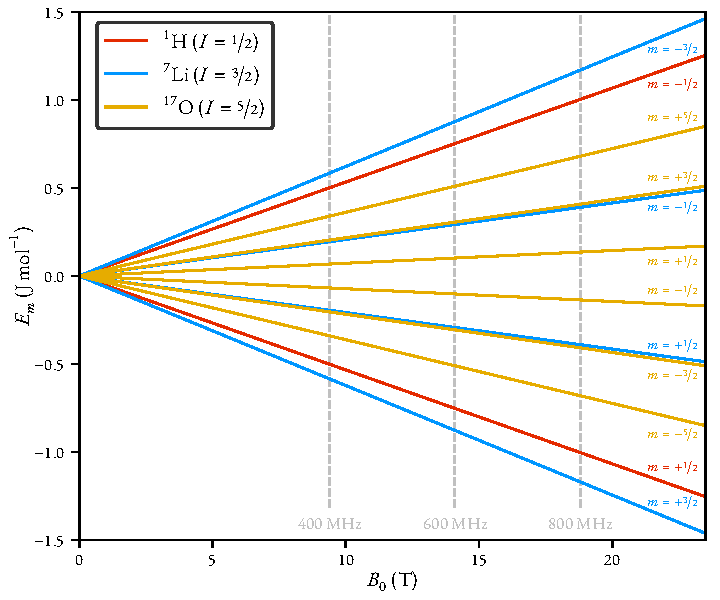
\includegraphics{energy_levels/energy_levels.pdf}%
    \caption[%
        The variation of energy of the spin states of \ch{^1H},
        \ch{^7Li}, and \ch{^{17}O} with external magnetic
        field strength.
    ]{%
        The variation of energy of the spin states of \ch{^1H},
        \ch{^7Li}, and \ch{^{17}O} with external magnetic
        field strength ($B_0$) up to \qty{23.5}{\tesla}, which is
        approximately the strength of a \qty{1}{\giga \hertz} \ac{NMR} magnet.
        Three common field strengths for commercial NMR magnets are indicated:
        \qty{9.40}{\tesla} (\qty{400}{\mega\hertz}), \qty{14.10}{\tesla}
        (\qty{600}{\mega\hertz}), and \qty{18.79}{\tesla}
        (\qty{800}{\mega\hertz}). \correction{Note the relative ordering of the spin states
        for \textsuperscript{1}H and \textsuperscript{7}Li (with positive
        $\gamma$) versus \textsuperscript{17}O (with negative  $\gamma$).}
    }%
    \label{fig:energy_levels}%
\end{figure}%
\ac{NMR} samples comprise a vast ensemble of equivalent spin systems, and it is
the macroscopic properties of the sample that are observed.
At thermal equilibrium, the various spin states will be disproportionately
populated\,---\,albeit to a meager extent due to the small
relative energies involved\,---\,in accordance with the Boltzmann
distribution, with lower energy states being more heavily populated. For
example, an ensemble of
non-interacting spin-$\nicefrac{1}{2}$ nuclei with $\gamma > 0$, such as
\ch{^1H}, will have a more populated $m = +\nicefrac{1}{2}$ (\textalpha) state,
relative to the $m = -\nicefrac{1}{2}$ (\textbeta) state.  Due to the
population imbalance, the ensemble acquires a net (bulk) magnetic moment
$\symbf{M}$, given by the sum of all the individual spin moments:
\begin{equation}
    \symbf{M} = \sum\limits_{s=1}^{S} \symbf{\mu}_s,
\end{equation}
where $S \gg 1$ is the number of spins in the ensemble.
At equilibrium, the $x$- and $y$-components of the bulk magnetisation are zero:
\begin{equation}
    \sum_{s=1}^{S} \mu_{x,s} = \sum_{s=1}^{S} \mu_{y,s} = 0,
\end{equation}
such that the bulk magnetisation is collinear with the field direction, with a
magnitude $M_0$.

\correction{
    The fractional population of the state $m$ is given by:
    \begin{equation}
        p_{m} = \frac{\exp\left(\frac{m\hbar \gamma B_0}{k_{\text{B}} T}\right)}
        {\sum\limits_{m} \exp\left(\frac{m\hbar \gamma B_0}{k_{\text{B}} T}\right)},
        \label{eq:boltzmann}
    \end{equation}
    where $k_{\text{B}}$ is the Boltzmann constant
    (\qty{1.381e-23}{\joule\per\kelvin}),
    and $T$ is the sample temperature.
    N.B. $\sum_{m=-I}^I p_m = 1$.
    Given typical values of $\gamma$ ($\approx\!\!\qty{1e8}{\per\tesla\per\second}$) and
    $B_0$ ($\approx\!\!\qty{10}{\tesla}$),
    the inequality
    $\nicefrac{m\hbar\gamma B_0}{k_{\text{B}} T} \ll 1$ can be safely assumed
    at all temperatures used in solution-state \ac{NMR}. For this reason, the
    exponential terms in \cref{eq:boltzmann} may be approximated using a Taylor
    expansion truncated at the first-order term.
    Through this, it can be shown that the magnitude of the bulk magnetisation
    is given by
\begin{subequations}
    \begin{gather}
        M_0 = \sum_{s=1}^S \mu_{z,s} = S \hbar \gamma \sum_{m=-I}^{I} m p_m
            \approx \frac{S \gamma^2 \hbar^2 B_0 I (I + 1)}{3 k_{\text{B}} T}\\
        \implies M_0(I=\nicefrac{1}{2}) \approx
            \frac{S \gamma^2 \hbar^2 B_0}{4k_{\text{B}} T},%
        \label{eq:M0}%
    \end{gather}%
\end{subequations}%
}\label{corr:high-temp}%
To maximise experiment sensitivity, it is desirable to
study nuclei with high natural abundance (affecting $S$ for a given sample
concentration), and high
gyromagnetic ratio. Along with other favourable attributes such as its ubiquity
in organic molecules, \ch{^1H} is therefore by far the most popular nucleus to
study using \ac{NMR}, at least in solution-state contexts.

The bulk magnetisation experiences a torque induced by the magnetic field, with its
evolution described by
\begin{equation}
  \frac{\mathrm{d}\symbf{M}(t)}{\mathrm{d}t} = \symbf{M}(t) \times \gamma \symbf{B}(t).
  \label{eq:M-cross-B}
\end{equation}
The essence of \ac{NMR} is to manipulate and subsequently detect the evolution
of $\symbf{M}$. Manipulation is achieved by applying short bursts of \ac{RF}
radiation known as \emph{pulses} which perturb the net magnetic field away from
$\symbf{B}_0$. The contribution to the field induced by pulses is commonly
denoted $\symbf{B}_1$, such that at any given time
\begin{equation}
    \symbf{B}(t) = \symbf{B}_0 + \symbf{B}_1(t).
\end{equation}
Whenever the magnetisation vector is not collinear with the field vector\footnote{
    The cross product of two collinear vectors is $0$, so $\symbf{M}$ remains
    fixed when it is aligned with $\symbf{B}$, as is the case at equilibrium.
}, it
\emph{precesses} about the field vector. Free precession occurs
when the magnetisation is aligned away from the $z$-axis and $\symbf{B}_1 =
\symbf{0}$, leading to
\begin{equation}
  \frac{\mathrm{d}\symbf{M}(t)}{\mathrm{d}t} =
  -\gamma B_0 ( M_y(t) \symbf{i} -M_x(t) \symbf{j} + 0 \symbf{k}),
\end{equation}
where $\lbrace \symbf{i}, \symbf{j}, \symbf{k}\rbrace \in \mathbb{R}^3$ denote the
unit vectors along the laboratory $x$-, $y$-, and $z$-axes, respectively.
Under free precession, the magnetisation rotates about the $z$-axis (i.e.
$\symbf{B}_0$) at the \emph{Larmor frequency} $\omega_0 = -\gamma
B_0$.\footnote{
    While the \ac{SI} unit of magnetic field strength is the Tesla
    (\unit{\tesla}), when referring to the field strength that a spectrometer
    operates at, it is common to use \unit{\mega\hertz} instead. This refers to
    the Larmor frequency of a reference \proton\ nucleus at the
    given field strength. For example, a \qty{500}{\mega\hertz} spectrometer
    operates at a field strength of
    $\nicefrac{2 \pi \times \qty{5e8}{\per\second}}{\qty{2.6752e8}{\radian\per\tesla\per\second}}
    \approx \qty{11.74}{\tesla}$.
    \label{fn:MHz}
}

\correction{
The most common \ac{RF} pulses used in \ac{NMR} are linearly polarised and
sinusoidally modulated. As an example, a pulse which is polarised along
the laboratory $x$-axis takes the form
\begin{equation}
    \symbf{B}_1(t) = 2 B_1 \cos(\omega_{\text{RF}} t + \phi_{\text{RF}}) \symbf{i},
    \label{eq:linear-pulse}
\end{equation}
where $B_1 \ll B_0$ is the strength of the \emph{resonant} \ac{RF} field
(\emph{vide infra}),
$\omega_{\text{RF}}$ is its angular frequency,
and $\phi_{\text{RF}}$ is its phase.
This pulse can instead be thought of as the
superposition of two circular fields, rotating with opposite senses:
\begin{equation}
    \begin{split}
        \symbf{B}_1(t) = B_1(%
                \cos(\omega_{\text{RF}} t + \phi_{\text{RF}}) \symbf{i} +
                \sin(\omega_{\text{RF}} t + \phi_{\text{RF}}) \symbf{j}
            )\\%
            + B_1(%
                \cos(\omega_{\text{RF}} t + \phi_{\text{RF}}) \symbf{i} -
                \sin(\omega_{\text{RF}} t + \phi_{\text{RF}}) \symbf{j}
            ).
    \end{split}
    \label{eq:B1}
\end{equation}
Assuming that $\lvert \omega_{\text{RF}} \rvert$ and $\lvert \omega_0 \rvert$
are close in value, the circular component which rotates with the same
sense as the spin magnetisation is said to be \emph{on resonance}. The
component which rotates with the opposite sense has a negligible effect on
the magnetisation in most circumstances.
An \ac{RF} pulse may therefore be considered to take the following form to a
high degree of accuracy:
}\label{corr:rf-pulse}
\begin{equation}
    \symbf{B}_1(t) =
        B_1\left(
            \cos(\omega_{\text{RF}} t + \phi_{\text{RF}}) \symbf{i} +
            \sin(\omega_{\text{RF}} t + \phi_{\text{RF}}) \symbf{j}
        \right),
        \label{eq:B1}
\end{equation}
A great simplification to \cref{eq:M-cross-B} is realised by
considering a frame of reference which, rather than being static, rotates at
$\omega_{\text{RF}}$, as this makes the \ac{RF} field appear to be
time-independent. This is referred to as the \emph{rotating frame}, and leads
to \cref{eq:M-cross-B} being recast as
\begin{subequations}
    \begin{gather}
        \frac{\mathrm{d}\tilde{\symbf{M}}(t)}{\mathrm{d}t} = \tilde{\symbf{M}}(t) \times \gamma \tilde{\symbf{B}}(t),\\
        \tilde{\symbf{B}}(t) =
            B_1 \cos(\phi_{\text{RF}}) \tilde{\symbf{i}} +
            B_1 \sin(\phi_{\text{RF}}) \tilde{\symbf{j}} +
            \Updelta B_0 \tilde{\symbf{k}},\\
        \Updelta B_0 = -\frac{\Omega}{\gamma},\\
        \Omega = \omega_0 - \omega_{\text{RF}},\\
        \correction{
            \tilde{\symbf{i}} = \cos(\omega_{\text{RF}} t) \symbf{i} +
                \sin(\omega_{\text{RF}} t) \symbf{j},
            }\\
        \correction{
                \tilde{\symbf{j}} = \cos(\omega_{\text{RF}} t) \symbf{j}
                - \sin(\omega_{\text{RF}} t) \symbf{i},
            }\\
        \tilde{\symbf{k}} = \symbf{k}
    \end{gather}%
    \label{eq:rot-frame}%
\end{subequations}%
The tilde has been used to distinguish quantities in the rotating frame from
their laboratory frame counterparts.
$\Omega$ is the \emph{offset} of the spin
magnetisation. When $\Omega = \qty{0}{\radian\per\second}$, the \ac{RF} field is
perfectly on resonance, and at times when it is not being applied, the
magnetisation vector appears to be static in the rotating frame.

\Cref{eq:rot-frame} implies that at times when $\tilde{\symbf{M}}$ is tilted
away from $z$-axis, and not \ac{RF} pulse is being applied, it rotate
indefinitely about the $z$-axis with a
frequency of $\Omega$. However, in reality the system is driven to re-establish
its thermal equilibrium state:
\begin{equation}
    \symbf{M}_{\text{eq}} \equiv \tilde{\symbf{M}}_{\text{eq}} = 0 \symbf{i} + 0\symbf{j} + M_0 \symbf{k}.
\end{equation}
The process by which
this occurs is called \emph{relaxation}.
\correction{
    \label{corr:relaxation}
    Spin relaxation is driven by the stochastic motion of the molecules in
    the sample, which give rise to variations in the magnetic fields
    present. The fields induced by molecular motion vary with time, and average
    to zero. Furthermore, in different locations within the sample, the
    variation in these fields with time is uncorrelated. As a result, these
    fields are often referred to as \emph{local} fields.
    The presence of time-varying local fields in the sample lead to a number of
    mechanisms that contribute to relaxation. These mechanisms are often classified
    based on whether or not they are associated with an energy transfer:
    \begin{itemize}
        \item \emph{Adiabatic interactions} do not require a transfer of energy
            between a spin system of interest and its surroundings\footnote{
                \correction{
                    The surroundings of a particular spin system of interest is
                    often referred to as the \emph{lattice}, which contains all
                    degrees of freedom in the sample other than those of the spin
                    system itself, including motional degrees of freedom of all
                    molecules in the system, and the spin energy levels of all
                    other molecules.
                }
            }. Molecular motion results in the $z$-component of the magnetic
            field experienced by a given spin to vary with time.
            The associated Larmor frequency of the spin is perturbed in
            accordance with this field variation.
            Spins in different locations, experiencing
            differing local $z$-field fluctuations, will gradually lose
            synchronisation with each other (i.e. become \emph{dephased}) as
            their instantaneous Larmor frequencies are non-equivalent. The
            effect of this is for the transverse component of the bulk
            magnetisation to decay. Hence, adiabatic interactions contribute to
            \emph{transverse relaxation}, also referred to as \emph{spin-spin
            relaxation}.
        \item \emph{Nonadiabatic interactions} involve the transfer of energy
            between a spin and its surroundings. Molecular motion which leads
            to varying transverse ($xy-$) magnetic fields with a component that
            fluctuates at the spin's Larmor frequency is able to induce such an
            energy transfer. This mechanism drives the relative populations of
            the spin's energy levels towards their equilibrium configuration,
            restoring the $z$-component of the bulk magnetisation.
            As such, nonadiabatic interactions contribute towards
            \emph{longitudinal relaxation}, also referred to as
            \emph{spin-lattice relaxation}.
            Furthermore, due to the finite lifetimes of the spin states,
            their associated energies are not perfectly defined, in accordance
            with the Heisenberg uncertainty principle. Because of this,
            nonadiabatic interactions also contribute towards transverse
            relaxation.
    \end{itemize}
    In the Bloch model, the influence of longitudinal and transverse relaxation are
    accounted for by the incorporation of two processes with respective rate
    constants $R_1$ and $R_2$ (both with units of \unit{\per\second}). These
    processes are often described in terms of relaxation times
    instead: $T_i \coloneq \nicefrac{1}{R_i}, i \in \lbrace 1, 2\rbrace$.  In
    the vast majority of situations, the rate of transverse relaxation is
    greater than that of longitudinal relaxation, i.e. $T_2 \leq
    T_1$~\cite[Section 11.9]{Levitt2007}. The rate of longitudinal relaxation
    places a strict limit on the rate of transverse relaxation: $T_2 \leq 2
    T_1$; if this were violated, during the evolution of the bulk magnetisation
    vector, its magnitude would surpass its magnitude at equilibrium, which is
    a physical impossibility~\cite{Traficante1991}.
    The introduction of relaxation is phenomenological in the Bloch model; the
    reversion of the spin system to equilibrium is included purely to ensure
    the model agrees with observation. More sophisticated theories invoking
    Liouville-space quantum mechanics can account for
    relaxation however~\parencites[Chapter 5]{Cavanagh2007}[Chapter 6]{Kuprov2023}{Goldman2001}{Kuprov2007}.
}

\begin{figure}
    \centering
    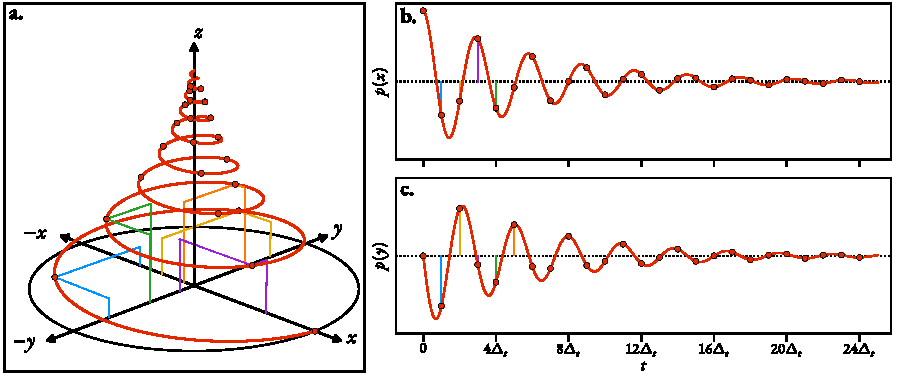
\includegraphics{quadrature_detection/quadrature_detection.pdf}
    \caption[
        The free evolution of the bulk magnetisation of an ensemble of
        spin-$\nicefrac{1}{2}$ nuclei according to the Bloch model.
    ]{
        \textbf{a.} An illustration of the free evolution of the bulk
        magnetisation of an ensemble of spin-$\nicefrac{1}{2}$ nuclei
        immediately after the application of a $\ang{90}_y$ pulse according to
        the Bloch model. The rate of transverse relaxation was set to be double
        that of longitudinal relaxation ($T_2 = \nicefrac{T_1}{2}$).
        The projections of the magnetisation vector onto the
        $x$- and  $y$-axes are plotted in panels \textbf{b.} and \textbf{c.},
        respectively. Modern \acs{NMR} spectrometers utilise quadrature
        detection, such that the $x$- and  $y$- projections of the time-varying
        magnetisation are sampled at regular time intervals, separated by
        $\Dt$.  The resulting \acs{FID} is given by the complex value $p(x) +
        \iu p(y)$.
    }\label{fig:quadrature}
\end{figure}

Everything has now been established to state the Bloch equations, which
describe the evolution of the bulk magnetisation of an ensemble of identical
spin-$\nicefrac{1}{2}$ nuclei in the rotating frame:
\begin{equation}
    \frac{\mathrm{d}\tilde{\symbf{M}}(t)}{\mathrm{d}t} =
    \begin{bmatrix}
        -R_2 & -\Omega & \omega_1 \sin(\phi_{\text{RF}}) \\
        \Omega & -R_2 & -\omega_1 \cos(\phi_{\text{RF}}) \\
        -\omega_1 \sin(\phi_{\text{RF}}) & \omega_1 \cos(\phi_{\text{RF}}) & -R_1
    \end{bmatrix}
    \tilde{\symbf{M}}(t)
    + R_1 M_0
    \begin{bmatrix}
        0 \\ 0 \\ 1
    \end{bmatrix},
\end{equation}
where $\omega_1 \coloneq -\gamma B_1$.
\Cref{fig:quadrature}.a depicts the
evolution of a bulk magnetisation vector after the application of an
\ac{RF} pulse with $\phi_{\text{RF}} = \nicefrac{\pi}{2}$, and an appropriate
combination of duration and power to induce a clockwise rotation of \ang{90}
about the $y$-axis; such a pulse is denoted $\ang{90}_{y}$.
Neglecting off-resonance effects, the magnetisation vector will land on the
$x$-axis, and evolve according to
\begin{subequations}
    \begin{gather}
        \tilde{M}_x(t) = M_0 \cos(\Omega t) \exp(-R_2 t),\\
        \tilde{M}_y(t) = M_0 \sin(\Omega t) \exp(-R_2 t),\\
        \tilde{M}_z(t) = M_0 (1 - \exp(-R_1 t)),
    \end{gather}
\end{subequations}
with $t=\qty{0}{\second}$ denoting the time that the magnetisation lands on the
$x$-axis.
During acquisition, the transverse components of the bulk magnetisation are
detected by the spectrometer probe circuitry
(Figures \ref{fig:quadrature}.b and \ref{fig:quadrature}.c), such that the
resulting signal, called the \acfi{FID}, is given by
\begin{subequations}
    \begin{gather}
        y(t) \propto \tilde{M}_+(t),\\
        \tilde{M}_+(t) = \tilde{M}_x (t) + \iu \tilde{M}_y (t) = M_0 \exp(\iu \Omega t - R_2 t).
    \end{gather}
\end{subequations}

\subsection{The NMR Spectrometer}

Modern \ac{NMR} spectrometers are capable of conducting a plethora of
experiments which can aide chemists.
In essence, a spectrometer comprises a high-field magnet, a probe, components
which are used to transmit \ac{RF} pulses to the probe, and components which
are used to process the resulting signal from the probe. A brief summary of
these is now given.

\subsubsection{The Magnet}
The static $\symbf{B}_0$ field is generated by a magnet which is composed of a
superconducting solenoid immersed in liquid helium; common materials used for
the solenoid include Nb-Ti alloy and Nb\textsubscript{3}Sn. To minimise the
extent of helium evaporation, the dewar containing the helium is lined with
a thermal radiation shield. The helium dewar is then surrounded by a larger
dewar containing liquid nitrogen,
\correction{which is finally encased in a vacuum chamber.\label{corr:vacuum}}
A bore passes through the $z$-direction of
the magnet, which is maintained at a user-specified temperature. Within the
bore sits the probe. Magnets with high field
strengths are desirable, as both the resolution ($\propto B_0$) and \ac{SNR}
($\propto B_0^{\nicefrac{3}{2}}$) of the data are affected. At the
time of writing, commercial spectrometers which operate at and above a
\ch{^1H} Larmor frequency of \qty{1}{\giga\hertz} (\qty{23.5}{\tesla}) exist,
though these are uncommon and are employed primarily for the study of large
biomolecules
\correction{and solid-state \ac{NMR}\label{corr:solid-state}}.
For most applications, including
the study of small molecules, spectrometers with more modest field strengths on
the order of \qty{100}{\mega\hertz} are typically adequate. Due to their cheap
operating costs and small size, ``benchtop'' \ac{NMR} spectrometers, which
comprise permanent magnets and typically operate on the order of
\qty{10}{\mega\hertz}, have also become popular in educational and
high-throughput settings~\cite{Giberson2021}.

To ensure a high spatial field homogeneity (a necessity for data with
acceptable resolution) a series of coils called \textit{shims} surround the
sample. Each coil produces a weak magnetic field with a specific spatial
profile in accordance with a spherical harmonic function; a collection of shims
can cancel out
\correction{small\label{corr:small-inhomog}}
inhomogeneities inherent to the main magnet~\cite[Chapter1, Appendix
B]{Webb2016}.
A field-frequency lock is used to ensure the stability of the
field. The lock is effectively a small \ac{NMR} spectrometer, tuned to a
specified isotope (typically \textsuperscript{2}H\footnote{
    \textsuperscript{2}H-enriched solvents are routinely used to make up
    \ac{NMR} samples. In \proton\ \ac{NMR} experiments, this ensures that an
    extremely intense signal due to the solvent does not dwarf the signals from
    other spins in the sample. This makes \textsuperscript{2}H a suitable
    nucleus to monitor by the lock, as it present in high concentrations, but
    rarely directly studied.
}), which monitors the resonance frequency of the isotope over
time. If the frequency begins to drift, the current in the $Z_0$ coil is
appropriately adjusted, which induces a constant change in field strength
throughout the sample volume.

\subsubsection{The Probe}
\correction{The probe sits inside the bore of the magnet and has a number of
responsibilities including holding the sample, regulating the sample temperature,
and housing the coils used to pulse the sample with \ac{RF}
radiation, as well as coils which are used to generate field
gradients\cite[Section 4.7]{Levitt2007}.\label{corr:probe}}
The \ac{RF} coils also receive the response from the sample during detection.
The principle source of data corruption in \ac{NMR} experiments is thermal
noise within the probe circuitry.  For this reason, cryogenic probes have
become a popular development, in which the coils and other probe electronics
are maintained at a very low temperature (typically about
$\qty{20}{\kelvin}$)~\cite{Kovacs2020}.

\subsubsection{The Transmitter}
The transmitter is responsible for the generation of \ac{RF} pulses
with specified power, timing and phase.
A synthesiser acts as an \ac{RF} source, producing a continuous carrier wave at
or very close to the Larmor frequency of the target nucleus. This frequency
($\omega_{\text{RF}}$) can be adjusted in order to determine the center of the
spectrum. The difference between the carrier frequency and the reference
``basic frequency'' of the spectrometer is referred to as the \emph{transmitter
offset} $\foff$.  The output of the synthesiser is gated to ensure pulses are
applied at the desired times. Attenuators/amplifiers then adjust the power
of the pulse, which travels to the probe.

\subsubsection{The Receiver}
During detection, the time-varying current induced in the probe coil by
the sample magnetisation \correction{travels to\label{corr:travel}} a receiver,
which comprises a series of components designed to convert the
analogue current to the digital \ac{FID} which is stored in computer memory.
One of the processes that the receiver is responsible for is \emph{quadrature
detection}~\cite[Section 13.6]{Keeler2010}, which ensures
\acp{FID} are frequency discriminated, i.e. that they possess the requisite
information to determine whether a given component in the \ac{FID} has a
frequency that is above or below the transmitter frequency.
This is achieved by splitting the signal from the probe into two channels. In
each channel, the signal, which is of a very high frequency
(\unit{\mega\hertz}), is mixed with a reference signal of frequency
$\omega_{\text{RF}}$. The mixing process results in a low-frequency
(\unit{\kilo\hertz}) signal being generated, along with a very high frequency
signal. The reference signal in one channel possesses a phase which
is shifted by \ang{90} relative to the other, such that the combined signal
constitutes a quadrature pair.
Both signals are then sent through a low-pass filter to remove
the high frequency component produced through mixing. Finally, an analogue to
digital converter translates the signal to the real and imaginary components of
a binary dataset which constitutes the \ac{FID}.

\subsection{The Structure of the \acs{FID}}
The result of running a \ac{1D} \ac{NMR} experiment is an \ac{FID} $\by \in
\mathbb{C}^N$ which is sampled at equally spaced points in time, with
consecutive samples separated by time $\Dt$:
\begin{equation}
    \begin{gathered}
        \by = \begin{bmatrix}
            y_0 & y_1 & y_2 & \cdots & y_{N-1}
      \end{bmatrix}\T\\
      \equiv
      \begin{bmatrix}
          y(t=0) & y(t=\Dt) & y(t=2\Dt) & \cdots & y(t=(N-1)\Dt)
      \end{bmatrix}\T,
    \end{gathered}
\end{equation}
where $y(t)$ is the (continuous) variation of the generated signal as a
function of time,
and $N$ (often a power of 2) is the number of points sampled. The inverse of
the sampling rate,
$\nicefrac{1}{\Dt}$ is the \correction{\emph{spectral width}\label{corr:sw}} $\fsw$ which
defines how large the range of samplable frequencies is, in accordance with the
Nyquist theorem~\cite{Shannon1949}.

\acp{FID} adopt the form of a summation of $M \in \mathbb{N}$ complex
exponentials; these will be referred to as \emph{signals} in this text. Each
signal will be subjected to damping due to transverse relaxation, which is
typically exponential in nature. An \ac{FID}
therefore takes the form\footnote{
    \correction{
        This provides an idealised model of an \ac{FID}, based on the
        underlying theory of the experiment. In reality, there is the possibility
        of significant deviations from this model being realised. One potential
        cause of this is the influence of magnetic field inhomogeneities, which
        will cause spectral peaks to deviate from having Lorentzian lineshapes
        (\cref{subsec:nmr-proc}). In cases where distortions to the data have
        occurred, techniques such as \emph{reference deconvolution}~\cite{Morris1997}
        can be used as a corrective measure in a bid to make the data agree more
        closely with this model.
    }\label{fn:ref-decon}
}
\begin{subequations}
    \begin{gather}
        y_n = x_n(\bth) + w_n \quad
            \quad \forall n \in \lbrace 0, 1, \cdots, N - 1 \rbrace,
            \label{eq:y=x+w} \\
        x_n(\bth) =
        \sumM \amexpphim \exp\left(
            (2 \pi \iu (f_m - \foff)- \eta_m ) n \Dt
        \right).
        \label{eq:x-1d}
    \end{gather}
    \label{eq:1d}%
\end{subequations}%
\cref{eq:1d} indicates that \iac{FID} comprises a deterministic contributions
from the evolution of the spin magnetisation $\bx$, as well as one from
experimental noise $\bw$ (\emph{vide infra}). Each signal which contributes to
$\bx$ is defined by four parameters:
\begin{itemize}
    \item Amplitude $a \in \mathbb{R}_{>0}$ ,
    \label{pg:param-constraints}
    \item Phase $\phi \in (-\pi, \pi]$ (\unit{\radian}),
    \item Frequency $f \in \left[\hspace*{2pt}\foff - \nicefrac{1}{2} \hspace*{2pt}
        \fsw, \foff + \nicefrac{1}{2} \hspace*{2pt}\fsw \right]$ (\unit{\hertz}),
    \item Damping factor $\eta \in \mathbb{R}_{>0}$ (\unit{\per\second}).
\end{itemize}%
\Iac{FID} can therefore be parameterised by the vector $\bth \in
\mathbb{R}^{4M}$:
\begin{equation}
    \bth =
    \begin{bmatrix}
        \symbf{a}\T & \symbf{\phi}\T & \symbf{f}\T & \symbf{\eta}\T
    \end{bmatrix}\T,
\end{equation}
where $\bda \in \mathbb{R}^M = [a_1 \hspace{2pt} a_2 \hspace{2pt} \cdots
\hspace{2pt} a_M]^{\mathrm{T}}$ is a vector of all amplitudes, $\bdphi \in
\mathbb{R}^M$ is a vector of all phases, etc.
A more concise alternative to \correction{\cref{eq:x-1d}}
involves the \emph{complex amplitudes} and \emph{signal poles} associated with
the \ac{FID}:
\begin{subequations}
    \begin{gather}
        x_n(\bth) = \sumM \alpha_m^{\vphantom{n}} z_m^n,\\
        \alpha_m = \amexpphim,\\
        z_m = \exp\left(
            \left(2 \pi \iu \left(f_m - \foff\right) - \eta_m\right) \Dt
        \right).\label{eq:signal-pole}
    \end{gather}
    \label{eq:x-alpha-z}%
\end{subequations}
The respective influences of the four parameters on a signal in the time-domain
are depicted in Figures \ref{fig:amp-phase-freq-damp}.a1 to
\ref{fig:amp-phase-freq-damp}.d1.
\begin{figure}
    \centering
    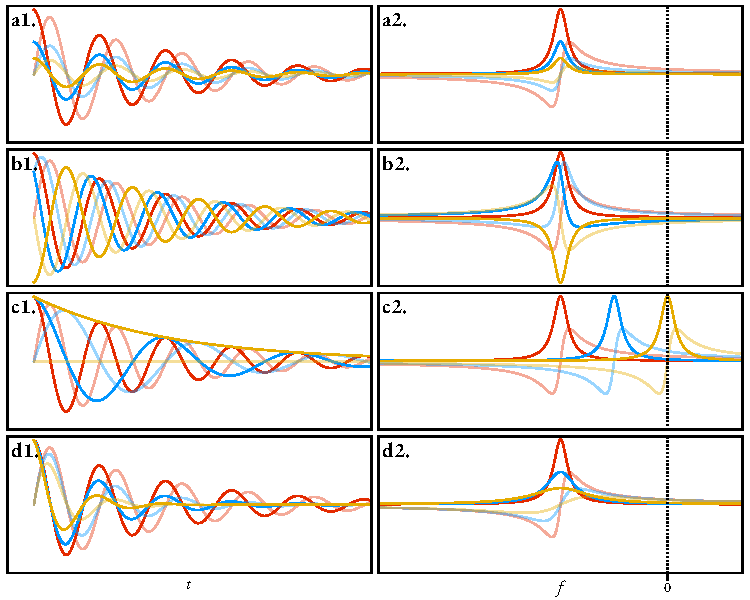
\includegraphics{amp_phase_freq_damp/amp_phase_freq_damp.pdf}
    \caption[
        The influence of the four parameters associated
        with an exponentially damped complex sinusoidal signal in both the
        time-domain and the Fourier-domain.
    ]{
        The influence of the four parameters associated
        with an exponentially damped complex sinusoidal signal in both the
        time-domain (a1 to d1) and Fourier-domain (a2 to d2).
        The red signal is generated with the same parameters across all panels:
        $a = a_{\text{red}}$, $\phi = 0\,\unit{\radian}$, $f = f_{\text{red}}$,  $\eta =
        \eta_{\text{red}}$.  The blue and yellow signals were produced by
        altering one parameter out of the four.
        \textbf{a.} $a_{\text{yellow}} = \nicefrac{1}{2} a_{\text{blue}} =
        \nicefrac{1}{4} a_{\text{red}}$.
        \textbf{b.}
        $\phi_{\text{blue}} = \nicefrac{\pi}{4}\,\unit{\radian}$,
        $\phi_{\text{yellow}} = \pi\,\unit{\radian}$.
        \textbf{c.}
        $f_{\text{blue}} = \nicefrac{1}{2} f_{\text{red}}$,
        $f_{\text{yellow}} = 0$.
        \textbf{d.}
        $\eta_{\text{yellow}} =
        \nicefrac{1}{2}\eta_{\text{blue}} =
        \nicefrac{1}{4}\eta_{\text{red}}$.
        The real and imaginary components of each signal are plotted, with the
        imaginary component being paler than its real counterpart.
    }
    \label{fig:amp-phase-freq-damp}%
\end{figure}

Multidimensional experiments~\cite[Chapter 4]{Cavanagh2007} involve
incrementing one or more delays within a
pulse sequence, in order to obtain an array of \ac{1D} \acp{FID}. In a
$D$-dimensional dataset, each contributing signal is parameterised by an
amplitude and phase as before, along with $D$ distinct frequencies and damping
factors, such that a general parameter vector  $\bth \in \mathbb{R}^{2(1+D)M}$
is given by
\begin{equation}
    \bth =
    \begin{bmatrix}
    \symbf{a}\T &
    \symbf{\phi}\T &
    {\bdfone}\T &
    \cdots &
    {\bdfD}\T &
    {\bdetaone}\T &
    \cdots &
    {\bdetaD}\T
    \end{bmatrix}\T,
    \label{eq:theta}
\end{equation}
where $\bdfD$ and $\bdetaD$ are the frequencies and damping factors in the
actively acquired (direct) dimension, and $\lbrace \bdfone, \cdots,
\bdfDminusone \rbrace$ and
$\lbrace \bdetaone, \cdots, \bdetaDminusone \rbrace$ are those of the indirect
dimension(s).
Indirect dimensions can exhibit different forms of evolution, depending on
the precise nature of the pulse sequence, of which two are very
common~\cite[Section 4.3.4]{Cavanagh2007}. \acp{FID} whose constituent signals
evolve according to $\cos(2 \pi f t)$ or $\sin(2 \pi f t)$ modulate the
amplitude of the direct dimension across increments, while those whose signals
evolve according to $\exp(2 \pi \iu f t)$ and $\exp(-2 \pi \iu f t)$ modulate
the phase instead.
For experiments which produce amplitude-modulated \acp{FID},
both the cosine and sine forms should be acquired if possible, as this ensures
that spectra with desirable properties can be generated. The same is true for the positive
and negative forms when phase-modulated \acp{FID} are acquired (\emph{vide
infra}). In general, a $D$-dimensional \ac{FID} $\bY \in \mathbb{C}^{\None
\times \cdots \times \ND}$ can be expressed as
\begin{subequations}
    \begin{gather}
        \ynonenD = \xnonenD(\bth) + \wnonenD,\\
        \xnonenD
            = \sumM \amexpphim \prodD
            \zeta^{(d)}\left(2 \pi \left(f^{(d)}_m  - \foffd\right) \nd \Dtd\right)
            \exp\left(-\eta^{(d)}_m \nd \Dtd\right),\\
        \zeta^{(d)}(\cdot)
        \begin{cases}
            = \exp(\iu\cdot) & d = D \\
            \in \left\lbrace \cos(\cdot), \sin(\cdot), \exp(\iu\cdot) \exp(-\iu\cdot)\right\rbrace & \text{otherwise}
        \end{cases}.
    \end{gather}
    \label{eq:general-fid}%
\end{subequations}%

It is typical to assume that the data is corrupted by an array of \ac{AWGN},
i.e. the noise instances are described by a complex normal distribution with
mean 0, and pairs of noise instances are statistically independent, regardless
of their time separation:
\begin{subequations}
    \begin{gather}
        \wnonenD \sim
        \mathcal{N_C}\left(0, 2\sigma^2\right) \\
        \begin{gathered}
            \implies \Re\left(\wnonenD\right) \upmodels \Im\left(\wnonenD\right),\\
             \Re\left(\wnonenD\right) \sim \mathcal{N}\left(0, \sigma^2\right),\\
             \Im\left(\wnonenD\right) \sim \mathcal{N}\left(0, \sigma^2\right). \\
        \end{gathered}
    \end{gather}
\end{subequations}
The extent by which \iac{FID} is corrupted by noise is given by its \acf{SNR}:
\begin{equation}
    \SNR\left(\bY\right) \coloneq
        \frac{1}{2 N_{\text{tot}} \sigma^2}
        \sum_{\none=0}^{\None-1} \cdots \sum_{\nd=0}^{\ND-1}
        \left \lvert \xnonenD \right \rvert^2,
        \label{eq:snr}
\end{equation}
where $N_{\text{tot}} \coloneq \None \times \cdots \times \ND$ is the total
number of points the \ac{FID} comprises. Due to the large dynamic range
observed for the \ac{SNR} across datasets, it is common to express it using a
logarithmic scale instead, in units of decibels (\unit{\deci\bel}):
\begin{equation}
    \SNR_{\unit{\deci\bel}} \coloneq 10 \log_{10} \left(\SNR\right).
    \label{eq:snr-db}
\end{equation}

\section{An Overview of NMR Data Analysis}
To gain insights from \ac{NMR} experiments on the chemical system of interest,
extraction of the defining parameters $\bth$ is necessary, though the majority
of \ac{NMR} users are unlikely to think about the process of \ac{NMR} analysis
in this way. For example:
\begin{itemize}
    \item An understanding of the chemical environments of atoms in a molecule
        can be gained by considering the chemical shifts of the various peaks
        in the spectra, which are a proxy for the \ac{FID} frequencies
        $\symbf{f}$.
    \item  The relative stoichiometries\note{does this make sense?} of a
        molecule can be elucidated by inspecting the integrals of spectral
        peaks, which are directly related to the \ac{FID} amplitudes $\bda$
\end{itemize}

\note{
    \begin{itemize}
        \item Typical approach to analysing the data (FT, peak pick, integrate, baseline correction, window functions, zero-filling etc),
        \item Estimation techniques: LP, SVD techniques, iterative techniques (AMARES, VARPRO), Bayesian techniques (CRAFT), ML techniques
    \end{itemize}
}

\subsection{Conventional NMR Analysis}
\label{subsec:nmr-analysis}
The conventional route to interpret \ac{NMR} experiments is to
transform the \ac{FID} into the frequency domain, producing an
\ac{NMR} spectrum. This is achieved through application of the \acfi{FT}:
\begin{subequations}
    \begin{align}
        &\text{Continuous case:} &&\FT(x(t))(F) =  \int_{0}^{\infty} x(t) \exp(
            -2 \pi \iu t F
            ) \mathrm{d} t
            \quad \forall t \in \mathbb{R},\\
        &\text{Discrete case:} &&\FT( \symbf{x} )_n =  \sum_{k=0}^{N-1} x_k \exp \left(
            -\frac{2 \pi \iu k n}{N} \right)
            \quad \forall n \in \lbrace 0, \cdots, N-1 \rbrace.
    \end{align}
\end{subequations}
The \ac{FT} of a continuous exponentially-damped complex sinusoid
takes the form of a \emph{Lorentzian}\footnote{
    An upshot of only possessing data for $t \geq 0$ is
    that the \ac{FT} of an \ac{FID} features a vertical offset,
    such that the baseline does not sit at 0\cite{Tang1994}. This is corrected
    by halving the initial point of the \ac{FID} prior to \ac{FT}.
}:
\begin{subequations}
    \begin{gather}
        s(F) = \FT\left(
            a \exp(\iu \phi) \exp((2 \pi \iu f - \eta)t)
            \right)(F),\\
        s(F) = \frac{a \exp(\iu \phi) }
            {\eta + 2 \pi \iu (f - F)}.
    \end{gather}
\end{subequations}
When $a = \phi = 0$, this function is equivalent to the (unnormalised) \ac{pdf}
of the Cauchy distribution. The \ac{FT} is a linear function, such that the
\ac{FT} of a summation of signals is equivalent to the summation of the
\acp{FT} of each signal. A corollary is that an \ac{NMR} spectrum comprises a
series of Lorentzian ``peaks'', located at the frequencies of all the signals
in the \ac{FID}:
\begin{equation}
    s\left(F\right) = \sum_{m=1}^{M}
    \frac{\amexpphim}
    {\eta_m + 2 \pi \iu (f_m - F)}.
    \label{eq:ft-summation}
\end{equation}
The \ac{FT} is a very attractive means of processing \ac{NMR} data, as it
presents the data in a format which is human-interpretable, with the basic
rules describing how chemical structure is mapped to \ac{NMR} spectral
properties being a fundamental skill that virtually all experimental chemists
require\cite{Hore2015b}. Due to innate properties of the \ac{NMR} experiment,
as well as features arising from analysing a discrete signal, the raw output
from an \ac{NMR} experiment often leads to spectra with undesirable
characteristics without any extra manipulation. Extra processing
steps that are frequently applied to \ac{NMR} data are now outlined, in the
order that they are applied to the data. Note that apodisation and zero filling
are applied to the \ac{FID} (prior to \ac{FT}), while phase correction and
baseline correction are applied to the spectrum (after \ac{FT}).

\begin{figure}
    \centering
    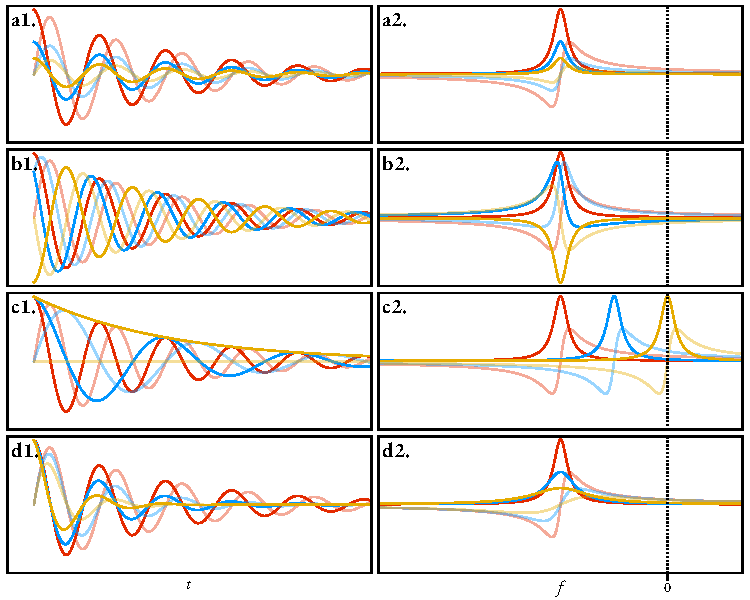
\includegraphics{amp_phase_freq_damp/amp_phase_freq_damp.pdf}
    \caption[
        An illustration of the influence of the four parameters associated
        with an oscillator in both the time-domain nels and Fourier-domain.
    ]{
        An illustration of the influence of the four parameters associated
        with an oscillator in both the time-domain (panels \textbf{a1.} --
        \textbf{d1.}) and Fourier-domain (panels \textbf{a2.} -- \textbf{d2.}).
        The red signal is generated with the same parameters across all panels:
        $a = a_{\text{red}}$, $\phi = 0$, $f = f_{\text{red}}$,  $\eta =
        \eta_{\text{red}}$.  The blue and yellow signals were produced by
        altering one parameter out of the four.
        \textbf{a.} $a_{\text{yellow}} = \nicefrac{1}{2} a_{\text{blue}} =
        \nicefrac{1}{4} a_{\text{red}}$.
        \textbf{b.}
        $\phi_{\text{blue}} = \nicefrac{\pi}{4}$,
        $\phi_{\text{yellow}} = \pi$.
        \textbf{c.}
        $f_{\text{blue}} = \nicefrac{1}{2} f_{\text{red}}$,
        $f_{\text{yellow}} = 0$.
        \textbf{d.}
        $\eta_{\text{blue}} = \nicefrac{1}{2}\eta_{\text{red}}$,
        $\eta_{\text{yellow}} = \nicefrac{1}{4}\eta_{\text{red}}$.
        The real and imaginary components of each signal are plotted, with the
        imaginary component being paler than its real counterpart.
    }
    \label{fig:amp-phase-freq-damp}
\end{figure}

\subsubsection{Apodisation}
Apodisation refers to the process of mutating a signal by multiplying it with a
specified function, often called a \emph{window function}, in order to enhance
a certain property. Apodisation is employed to improve either the sensitivity
or the resolution of the final spectrum, albeit at the cost of worsening the
other feature. There is no such thing as a free lunch after all.

\paragraph{Sensitivity Enhancement} As \iac{FID} progresses with time, the
contributions from the desirable signal ($\bx$) and experimental noise ($\bw$)
becomes more
weighted towards the noise, as spin relaxation phenomena dampen the signal. As
such, multiplying the \ac{FID} with a function which is initially large and
gets progressively smaller with time can be used to enhance the \ac{SNR} of the
\ac{FID}. The most common function to achieve this is the negative exponential
such that a given point is multiplied by $\exp(-\nicefrac{k n}{N - 1})$.
$k$ is referred to as the line broadening factor, since the increased dampening
applied to the signal causes the linewidth of the spectral peaks to increase
(see panel d of Figure \ref{fig:amp-phase-freq-damp}). As such, peaks become
more poorly resolved.

\paragraph{Resolution Enhancement} By contrast, resolution enhancement can be
achieved by applying a window function that artificially reduces the rate of
oscillator decay, by suppressing points that are early in the \ac{FID}. Popular
examples of window functions for resolution enhancement are the Lorentz-Gauss
function, which bestow a sharper, Gaussian shape to the peaks, and the
sine-bell, which is commonly used in multidimensional experiments. Since the
initial points in the \ac{FID} are attenuated these window functions reduce the
sensitivity of the resulting spectra.

By being defined to decay to a sufficiently small value, or $0$, at the end of
the \ac{FID}, window functions are also able to suppress \emph{truncation
artefacts}, which appear when the \ac{FID} still possesses appreciable signal
amplitude at the end of the acquisition period. Truncated \acp{FID} produce
spectra with peaks of a form that is akin to the convolution of the \ac{FT} of
the untruncated \ac{FID}, with the \ac{FT} of a box-function, which takes the
form of a sinc function ($\nicefrac{\sin(x)}{x}$). The resulting artefacts in
spectra are often referred to as \emph{sinc wiggles} for this reason.

\subsubsection{Zero filling}
\note{TODO}

\subsubsection{Phase correction}
The real and imaginary components of \eqref{eq:ft-summation} are as follows:
\begin{subequations}
    \begin{gather}
        \Re(s(F)) = \sum_m
        a_m (\cos(\phi_m) \mathcal{A}_m(F) + \sin(\phi_m) \mathcal{D}_m(F)),\\
        \Im(s(F)) = \sum_m
        a_m (\sin(\phi_m) \mathcal{A}_m(F) - \cos(\phi_m) \mathcal{D}_m(F)),
    \end{gather}
\end{subequations}
where $\mathcal{A}_m$ and  $\mathcal{D}_m$ denote \emph{absorption} and
\emph{dispersion} Lorentzians, respectively:
\begin{subequations}
    \begin{gather}
        \mathcal{A}_m(F) = \frac{\eta_m}{\eta_m^2 + 4 \pi^2 (f_m - F)^2},\\
        \mathcal{D}_m(F) = \frac{2 \pi (f_m - F)}{\eta_m^2 + 4 \pi^2 (f_m - F)^2}.
    \end{gather}
\end{subequations}
As illustrated most clearly in panel c2 of Figure
\ref{fig:amp-phase-freq-damp}, a peak with an absorption lineshape is far more
desirable than one with a dispersion lineshape for two key
reasons: (a) its maximum corresponds to the oscillator frequency, while a
dispersion Lorentzian has a magnitude of $0$ at the oscillator frequency (b)
they decay more rapidly towards $0$ and are therefore more resolved. Generating
a spectrum where all peaks possess absorption Lorentzians is therefore desired,
which is possible if all signal have a phase of \ang{0}, which leads to
\begin{subequations}
    \begin{gather}
        \Re(s(F)) = \sum_m a_m \mathcal{A}_m(F),\label{eq:absorption}\\
        \Im(s(F)) = -\sum_m a_m \mathcal{D}_m(F).\label{eq:dispersion}
    \end{gather}
\end{subequations}
 Fortunately, for the majority of \ac{NMR} experiments\footnote{
     An example of an exception to this rule is when \acl{FS} pulses are applied,
     which generate datasets with quadratic phase behaviour. This is discussed
     in more detail in Section \ref{sec:bbqchili}.
}, the contributing signals possess phases which depend linearly on their
frequencies, i.e.
\begin{equation}
    \phi_m = \Phi_0 + \Phi_1 f_m,
\end{equation}
where $\Phi_0, \in (-\pi, \pi]$ and $\Phi_1 \in \mathbb{R}$ are zero- and
first-order phase terms. A feature of all \ac{NMR} processing platforms is the
ability to perform phase-correction, in which the user determines
$\Phi_0$ and $\Phi_1$ by inspecting the appearance of the spectrum
$\symbf{s}_{\phi}$ for different values of $p_0$ and  $p_1$, according to
\begin{equation}
    s_{\phi,n} = s_n
    \exp\left(\iu \left(p_0 + \frac{p_1 n}{N - 1}\right)\right),
\end{equation}
in an attempt to give all peaks in the spectrum absorption-mode lineshapes.

\subsubsection{Baseline correction}
The \emph{baseline} of an \ac{NMR} spectrum is used to describe regions where
no discernible peaks reside (i.e. only experimental noise exists).
Baseline distortion is used to describe scenarios when the baseline, rather
than exhibiting a flat profile with a moving average of zero, has a distorted
shape instead. There a number of potential causes of baseline distortion,
including acquisition starting at a time $\neq 0$, ``clipping'' of the initial
points due to excessive receiver gain, and ``baseline roll'' due to the
transient response of audio filters\parencites[Section~3.3]{Cavanagh2007}{Tang1994}.
Whatever the cause(s), it is typically the corruption of the initial points in the
\ac{FID} that causes baseline distortion.
It is common to apply baseline correction algorithm after phase correction has
been undertaken to negate any distortion. This involves multiplying
the spectrum with a high-order polynomial function, whose coefficients are
determined by an appropriate algorithm. A popular algorithm
involves the two-step procedure of (a) determining spectral regions which are
part of the baseline (b) fitting the baseline regions to a
polynomial\cite{Dietrich1991,Cobas2006}.

\subsection{Conventional analysis for multidimensional datasets}
\label{subsec:mulitdim}
As for \ac{1D} datasets, it is desirable that multidimensional \ac{NMR} spectra
feature peaks which are (a) frequency discriminated, and (b) comprise pure
absorption-mode lineshapes, in each dimension. Frequency discrimination describes
the ability to determine whether a particular resonance is at a frequency which
higher or lower than the frequency of the transmitter, which is in the middle
of the spectral window. As an illustration of how this can be achieved, \ac{2D}
signals comprising a single oscillator will be considered, with
amplitude $a = 1$,  phase $\phi = \ang{0}$, frequencies $\fone$ and $\ftwo$, and
damping factors $\etaone$ and  $\etatwo$.

\subsubsection{Amplitude-modulated signals}
It is clear that a cosine modulated signal, given by \eqref{eq:general-fid}
with $D=2$ and $\zeta^{(1)} = \cos(\cdot)$ cannot achieve frequency
discrimination, on account of the relation
\begin{equation}
    \cos\left(2 \pi \fone \tone\right) =
    \tfrac{1}{2} \left(\exp\left(2 \pi \iu \fone \tone \right) + \exp\left(-2 \pi \iu
    \fone \tone \right)\right)
\end{equation}
\ac{FT} of a cosine-modulated \ac{FID} in both dimensions leads to a spectrum
whose real component comprises two peaks, one at the true resonance frequency
$\left(\fone, \ftwo\right)$, and the other at the mirror-image frequency in the
indirect dimension, $(2\foffone - \fone, \ftwo)$. On top of this, the
peaks possess a mixture of absorption and dispersion character, with the
resultant peak shape often referred to as \emph{phase twist}\cite{Keeler1985}.
A spectrum of this form is presented in panel a of Figure \ref{fig:2d-lineshapes}.
It is possible to generate pure absorption peaks by applying \ac{FT} in the
direct dimension, setting the imaginary component to zero, and finally
applying \ac{FT} in the indirect dimension. The real component of the result
(panel b) is referred to as a \emph{double absorption} spectrum.

To achieve frequency discrimination, it is necessary to also possess the
analogous sine-modulated signal, for which $\zeta^{(1)} = \sin(\cdot)$, as this
in effect achieves quadrature detection in the indirect dimension. For
numerous multidimensional experiments, this can be achieved by repeating the
pulse sequence, with careful adjustments to the phases of particular pulses, in
a process referred to as \emph{phase cycling}\cite[Chapter 11]{Keeler2010}.
Applying the same processing as that which achieved the double absorption
spectrum for the cosine-modulated case generates a spectrum whose imaginary
component features two peaks, but with opposite signs (panel c) which is borne
out of the sine function being odd. It then becomes possible to generate a
frequency discriminated spectrum by subtracting the sine spectrum from the
cosine spectrum (panel d).

\begin{figure}
    \centering
    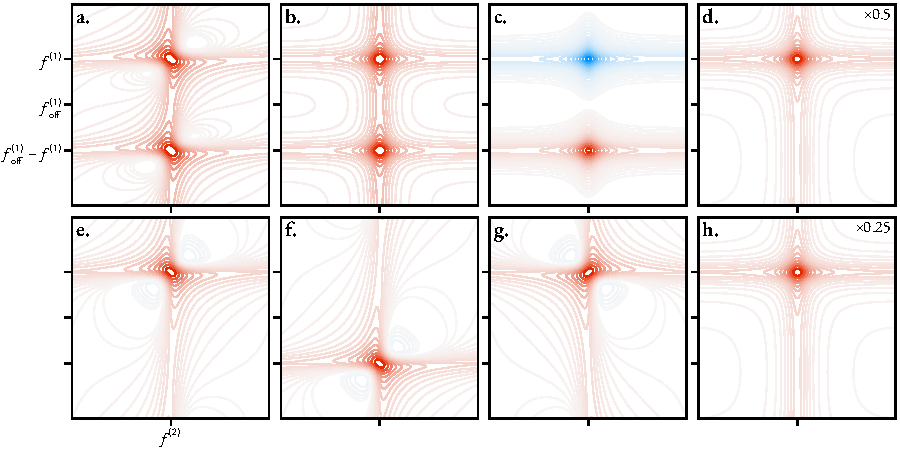
\includegraphics{2d_lineshapes/2d_lineshapes.pdf}
    \caption[
        Spectra acquired from amplitude- and phase-modulated \acs{2D} signals.
    ]{
        Spectra acquired from amplitude- and phase- modulated \acs{2D} signals.
        Red contour lines denote positive values, while blue contours denote
        negative values.
        \textbf{a.} The \ac{FT} of a cosine-modulated \ac{FID}, featuring peaks
        both at the true resonance frequency ($\fone$) and the mirrored
        frequency ($2\foffone - \fone_{\vphantom{off}}$), and with phase-twist lineshapes.
        \textbf{b.} Double-absorption spectrum generated by applying \ac{FT}
        in the direct dimension, setting the imaginary component to zero,
        applying \ac{FT} in the indirect dimension, and retaining the real
        component.
        \textbf{c.} Spectrum acquired with the same processing method as in
        \textbf{b.} but with a sine-modulated \ac{FID}, and with the imaginary
        component retained.
        \textbf{d.} The subtraction of the spectrum in \textbf{c.} from that in
        \textbf{b.} leads to a spectrum with frequency discrimination and a
        pure absorption lineshape.
        \textbf{e.} The \ac{FT} of a positive phase-modulated \ac{FID},
        exhibiting frequency discrimination, but with a phase twist shape.
        \textbf{f.} The \ac{FT} of a negative phase-modulated \ac{FID}.
        \textbf{g.} The spectrum in \textbf{f.} inverted along the indirect
        axis, about $\foffone$.
        \textbf{h.} The summation of \textbf{e.} and \textbf{g.} generates a
        spectrum with an absorption lineshape.
    }
    \label{fig:2d-lineshapes}
\end{figure}

\subsubsection{Phase-modulated signals}

A ``positive'' phase-modulated signal with the form $\zeta^{(1)} = \exp(\iu \cdot)$
(commonly referred to as \emph{hypercomplex}) is frequency-discriminated due to
its quadrature nature. However, direct \ac{FT} of such a signal in both
dimensions leads to a peaks with a phase-twist lineshape, with no means of
separating the absorption and dispersion contributions (panel e). Certain pulse
sequences, including \ac{2DJ} spectroscopy\cite{Aue1976,Morris2009} (see
Chapter \ref{chap:cupid}) and
\ac{COSY}\cite{Jeener1971,Jeener2016,Aue1976a} produce hypercomplex datasets,
and the conventional means of processing is simply to display the absolute
value of the spectrum, which while removing the phase twist shapes, produces
peaks with broad wings, due to the influence of the dispersive components. In
scenarios where it is possible, it is desirable to acquire the equivalent
``negative'' signal ($\zeta^{(1)} = \exp(-\iu \cdot)$), whose \ac{FT} leads to
a peak with the same phase twist form, but centered at $2\foffone - \fone$
(panel f). Inverting this spectrum in $\Fone$ (panel g), and summing with the
positive spectrum nullifies the dispersive contributions, generating a spectrum
with absorption lineshapes\cite{Davis1992} (panel h).

\subsection{Estimation Techniques for NMR Analysis}

\subsubsection{\Acl{LP}}

\Ac{LP}\cite{Stephenson1988,Koehl1999} is a procedure which is now widely used
in \ac{NMR} data analysis, often with the intention of (a) propagating the
\ac{FID} further in time in order to reduce the presence of truncation
artefacts and (b) correct the commonly corrupted initial points of the
\ac{FID}, as a means of improving the spectral baseline. The concept of \ac{LP}
stems from the idea that a deterministic signal, such as a \ac{1D} \ac{FID} can
be described as an \ac{AR} process, such that a given sample from the dataset
can be described by a linear combination of a certain number of previous
samples:
\begin{equation}
    \by \left[\none\right] = \sum_{l=0}^{L-1}
    \symbf{c}[l] \hspace{2pt} \by \left[ \none - l - 1\right] + \symbf{e} [l]
    \label{eq:forward-lp}
\end{equation}
$\forall \none \in \lbrace L, L + 1, \cdots, \None - 1 \rbrace$, where $L \in
\mathbb{Z}$ defines the order of the linear estimator, and $\symbf{c} \in
\mathbb{R}^{L}$ is a set of \emph{forward} \ac{LP} coefficients. $\symbf{e} \in
\mathbb{R}^L$ is a set of parameters, sometimes called the innovations, which
account of error in the \ac{LP} model. A datapoint can also be described by a
linear combination of a certain number of subsequent points, using the set of
\emph{backward} \ac{LP} coefficients $\symbf{b} \in \mathbb{R}^L$:
\begin{equation}
    \by \left[\none\right] = \sum_{l=0}^{L-1}
    \symbf{b}[l] \hspace{2pt} \by \left[ \none + l + 1\right] + \symbf{e} [l]
    \label{eq:backward-lp}
\end{equation}
$\forall \none \in \lbrace 0, 1, \cdots, \None - L - 1 \rbrace$. Determining
the \ac{LP} coefficients enables the estimation of \ac{FID} values beyond the
data actually acquired ($\none < 0$ and $\none > \None - 1$). It should be noted that
\eqref{eq:forward-lp} and \eqref{eq:backward-lp} are only valid for
\acp{FID} without any corruption from experimental noise. Noisy datasets are
instead an example of an \ac{ARMA} process. Despite this, due to the greater
simplicity of the \ac{AR} model, it is far more common to employ this. The most
common means of performing \ac{LP} is by solving the Yule-Walker
equations\cite{Yule1927,Walker1931},
which describe the relationship between the signal autocorrelation coefficients
and the \ac{LP} coefficients\cite[Section 3.3]{Koehl1999}, with the
Levinson-Durbin algorithm providing an efficient means of solving the
equations\cite{Levinson1946,Durbin1960}.

\note{Stuff below here has been copy-pasted from old document. Will need editing!}
\subsubsection{Signal-Noise Subspace Separation Techniques}

The Linear Prediction with Singular-Value Decomposition was proposed by Kumaresan and Tufts\cite{Kumaresan1982}. The core assumption of the method is that a given data point $y_n$ may be expressed as a linear combination of $L$ previous, or preceeding points:
\begin{equation}
  \begin{split}
    y_n &= b_1 y_{n+1} + b_2 y_{n+2} + \cdots + b_L y_{n+L}\\
    &= b_{-1} y_{n-1} + b_{-2} y_{n-2} + \cdots + b_{-L} y_{n-L}
  \end{split}
\end{equation}
where $b_l$($b_{-l}$), $\ l \in \{ 1, 2, \cdots, L \}$ are the backward(forward) prediction coeffiecients. For the backward prediction case, consider the follwing set of linear equations $\symbf{A} \symbf{b} = - \symbf{h}$:
\begin{equation}
  \label{lineqs}
  \begin{bmatrix}
    y_1^* & y_2^* & \cdots & y_L^*\\
    y_2^* & y_3^* & \cdots & y_{L+1}^*\\
    \vdots & \vdots & \ddots & \vdots\\
    y_{N-L}^* & y_{N-L+1}^* & \cdots & y_{N-1}^*\\
  \end{bmatrix}
  \begin{bmatrix}
    b_1\\
    b_2\\
    \vdots\\
    b_L
  \end{bmatrix}
  = -
  \begin{bmatrix}
    y_0^*\\
    y_1^*\\
    \vdots\\
    y_{N-L-1}^*
  \end{bmatrix}
\end{equation}
This equation can be augmented into the form $\symbf{A}^{\prime} \symbf{b}^{\prime} = \symbf{0}$, with $\symbf{A}^{\prime} = \left[ \symbf{h} \vert \symbf{A} \right]$ and $\symbf{b}^{\prime} = \left[1, \symbf{b}^{\mathrm{T}} \right]^{\mathrm{T}}$. For the noiseless data case (i.e. $y_n = x_n$), any row of $\symbf{A}^{\prime}$ can be written as the linear combination of $J$ linearly independent vectors $\symbf{f}_j,\ j \in \{1, 2, \cdots, J\}$\cite{Kumaresan1983}:
\begin{equation}
  \symbf{f}_j = \left[ 1, z_j^*, \left(z_j^2\right)^*, \cdots, \left(z_j^L\right)^* \right],
\end{equation}
meaning that the rank of $\symbf{A}^{\prime}$ is $J$, provided it posseses at least $J$ rows ($J \leqslant N - L$). The fact that $\symbf{b}^{\prime}$ lies in the null space of $\symbf{A}^{\prime}$ implies that $\symbf{f}_j \symbf{b}^{\prime} = 0$, such that the following holds:
\begin{equation}
  \label{lincom}
  1 + b_1 z_j^* + b_2 \left(z_j^2\right)^* + \cdots + b_L \left(z_j^L\right)^* = 0
\end{equation}
It should be noted that $L$ must satisfy $L \geqslant J$ to ensure the null space of $\symbf{A}^{\prime}$ has at least a dimension of 1.
Eqn. \ref{lincom} leads to a means of deriving the signal poles $z_j$ via polynomial $B(\zeta)$:
\begin{equation}
  B(\zeta) = 1 + b_1 \zeta^{-1} + b_2 \zeta^{-2} + \cdots + b_L \zeta^{-L},
\end{equation}
the zeros of which will occur whenever $\zeta = \left(z_j^{-1}\right)^*,\ j \in \{1, 2, \cdots, J\}$.

Of course, the prediction coefficient vector $\symbf{b}$ still needs to be determined. Eqn. \ref{lineqs} implies that the optimal vector can be determined by simple linear lest squares:
\begin{equation}
  \hat{\symbf{b}} = - \mathbf{A}^+ \symbf{h}.
\end{equation}
However, noise components of the signal will be incorporated into the solution of $\symbf{b}$. To avoid this, $\symbf{A}$ is moved from the signal-noise subspace to the signal subspace via filtration using Singular-Valued Decomposition:
\begin{equation}
  \symbf{A} = \symbf{U}
  \begin{bmatrix}
    \symbf{\Sigma}\\
    \symbf{0}
  \end{bmatrix}
  \symbf{V}^{\dagger} = \sum_{l=1}^R \sigma_l^{\vphantom{\dagger}} \symbf{u}_l^{\vphantom{\dagger}} \symbf{v}_l^{\dagger}
\end{equation}
where $R = \\mathrm{rank}(\symbf{A}) = \min(L, N)$. The matrix $\tilde{\symbf{A}}$ of rank $J$ with the closest relationship to $\symbf{A}$ is a Frobenius norm sense is given by\cite{Cadzow1988}:
\begin{equation}
  \tilde{\symbf{A}} = \sum_{l=1}^J \sigma_l^{\vphantom{\dagger}} \symbf{u}_l^{\vphantom{\dagger}} \symbf{v}_l^{\dagger}.
\end{equation}
Using the following relationship between a matrix's pseudoinverse and its SVD:
\begin{equation}
  \symbf{A}^+ = \symbf{V}
  \begin{bmatrix}
    \symbf{\Sigma}^+\\
    \symbf{0}
  \end{bmatrix}
  \symbf{U}^{\dagger},
\end{equation}
The optimal vector of prediction coeffiecients is determined by:
\begin{equation}
  \hat{\symbf{b}} = - \tilde{\symbf{A}}^+ \symbf{h} = - \sum_{l=1}^J \sigma_l^{-1 \vphantom{\dagger}} \symbf{v}_l^{\vphantom{\dagger}} \left[ \symbf{u}_l^{\dagger} \symbf{h} \right]
\end{equation}
Application: \cite{Barkhuijsen1985}

\note{HSVD, MPM, only gloss over MPM as it is described in detail in Chapter 2}

\subsubsection{Iterative Methods}

The \ac{VARPRO} method is an iterative approach to parameter estimation, developed by Golub and Pereyra\cite{Golub1973}, and applied to NMR signal analysis by van der Veen et al.\cite{VanDerVeen1988}. It relies on minimising the following quantity:
\begin{equation}
  \label{VARPRO_min}
  \hat{\symbf{\theta}} = \argmin_{\symbf{\theta}} \left \lVert \symbf{y} - \symbf{x}(\symbf{\theta}) \right \rVert^2
\end{equation}
The vector $\symbf{x}$ can be expressed in the following format:
\begin{equation}
  \label{VARPRO_Za}
  \symbf{x} =
  \begin{bmatrix}
    z_1^0 & z_2^0 & \cdots & z_J^0\\
    z_1^1 & z_2^1 & \cdots & z_J^1\\
    \vdots & \vdots & \ddots & \vdots\\
    z_1^{N-1} & z_2^{N-1} & \cdots & z_J^{N-1}\\
  \end{bmatrix}
  \begin{bmatrix}
    \alpha_1\\
    \alpha_2\\
    \vdots\\
    \alpha_J
  \end{bmatrix}
  = \symbf{Z}\symbf{\alpha}
\end{equation}
Using Eq. \ref{VARPRO_Za}, Eq. \ref{VARPRO_min} can be re-written as follows:
\begin{equation}
    \hat{\symbf{\theta}} = \argmin_{\symbf{\theta}} \left \lVert \symbf{y} - \symbf{Z}\symbf{\alpha} \right \rVert^2
\end{equation}
The complex amplitudes can be determined analytically as follows:
\begin{equation}
  \label{VARPRO_alpha}
  \hat{\symbf{\alpha}} \approx \left( \symbf{Z}^{\dagger} \symbf{Z} \right)^{-1} \symbf{Z}^{\dagger} \symbf{y} \equiv \symbf{Z}^+ \symbf{y}
\end{equation}
$\symbf{Z}^+$ is the Moore-Penrose pseudoinverse of matrix $\symbf{Z}$\cite{Penrose1955, Strang2018}. The VARPRO method determines the frequencies and damping factors via an iterative minimisation of:
\begin{equation}
  \hat{\left[\symbf{f}^{\mathrm{T}}, \symbf{\eta}^{\mathrm{T}}\right]}^{\mathrm{T}} = \argmin_{\left[\symbf{f}^{\mathrm{T}}, \symbf{\eta}^{\mathrm{T}}\right]} \left \lVert \symbf{y} - \symbf{Z}\symbf{Z}^+\symbf{y} \right \rVert^2
\end{equation}
which is achieved using the Levenberg–Marquardt algorithm\cite{Levenberg1944, Marquardt1963}. The amplitudes and phases are subsequently determined using Eq. \ref{VARPRO_alpha}. This means that the amplitudes and phases do not need initial guesses assocaited with them. Further specifications can be applied to the algorithm, reflecting the spectroscopist's knowledge of the signal under inspection. For example, if it is known that a certain set of resonances constitute a multiplet, the relative frequency differences and amplitudes will be known.

\ac{AMARES}\cite{Vanhamme1997}


\subsubsection{Bayesian Methods}
\ac{CRAFT}\cite{Krishnamurthy2013}
2D\cite{Krishnamurthy2017}
perspective\cite{Krishnamurthy2021}

\subsubsection{Machine Learning Methods}
\cite{Schmid2023}

\section{Overview of this work}

\subsection{Conception and motivation}
The central focus of this work is the development of a routine which performs
parametric estimation on \ac{NMR} datasets.
Motivation initially came from discussions within the NMR
Methodology Group in Manchester involving
Dr Mohammadali Foroozandeh and co-workers (notably Prof.  Gareth Morris and
Prof. Mathias Nilsson) while Dr Foroozandeh was a
Postdoctoral researcher there. The group were interested in generating pure
shift \ac{NMR} spectra from \ac{2DJ} datasets via appropriate post-processing
of the data.  While little progress was made when Dr Foroozandeh was based in
Manchester, he wished to continue with the project after moving to Oxford to
take up a research fellowship; I took the reins of the project when I joined
his nascent research group as a PhD student.

To ensure its applicability to \ac{2DJ} datasets, the following properties were
sought while devising what a suitable estimation routine would entail:

\paragraph{Support for \ac{1D} and \ac{2D} data}
The method should be able to analyse both \ac{1D} \acp{FID} and also
hypercomplex \ac{2D} \acp{FID} (the form which \ac{2DJ} datasets take).
\ac{2D} data should be analysed holistically,
rather than as successive \ac{1D} increments, as is the case in methods like
\ac{CRAFT}\cite{Krishnamurthy2017} and other previous approaches which will be
discussed later. This is since better signal resolution is often available when
both dimensions are considered at the same time; certain signals which exhibit
clear resolution in a \ac{2D} dataset may be heavily overlapping in \ac{1D}
data and are therefore more challenging if not impossible to quantify
accurately.

\paragraph{Time-domain based}
As discussed in \cref{subsec:multidim}, due to the hypercomplex nature of
\ac{2DJ} \acp{FID}, generating spectra with desirable absorption lineshapes is
not possible. Typically, resorting to displaying the spectra in magnitude-mode is
deemed optimal, as this overcomes the phase-twist peak lineshapes. However,
such spectra suffer from severe non-linearities and dispersion-mode
contributions, both of which make the task of estimating \ac{2DJ} data in the
Fourier domain challenging. For this reason, estimating the dataset by
considering its \ac{FID} rather than its spectrum is preferred.

\paragraph{Accessibility}
To achieve wide-spread adoption, especially by non-expert \ac{NMR} users,
the method should require minimal user intervention to perform effectively. As
such, a method requiring the specification of as little prior knowledge
about the data as possible is desired.
On top of this, the method should be available as software that users can gain
familiarity with easily.

\subsection{Thesis Overview}
The remainder of this thesis comprises the following chapters:
\begin{itemize}
    \item \textbf{\cref{chap:theory}} discusses the theory behind routines
        which can be applied to determine parameter estimates related to
        \ac{1D} and \ac{2D} \acp{FID}.
    \item \textbf{\cref{chap:results}} provides illustrations of the
        performance of the estimation routine on \ac{1D} \ac{NMR} datasets.
        Furthermore, means in which parametric estimation routine can be
        harnessed for two applications are explored:
        \begin{itemize}
            \item The analysis of amplitude-attenuated datasets, such as those
                derived from diffusion-, $T_1$- and $T_2$-measuring
                experiments (\cref{sec:seq}).
            \item Overcoming quadratic phase behaviour and baseline distortions
                associated with ultra-broadband excitation by a single
                \acl{FS} pulse (\cref{sec:bbqchili}).
        \end{itemize}
    \item \textbf{\cref{chap:cupid}} outlines a devised method, given the acronym
        \acs{CUPID}, for generating pure shift spectra from the estimation of
        \ac{2DJ} datasets.
    \item \textbf{\cref{chap:nmrespy}} describes the source code developed as
        part of this project, called \ac{EsPy}.
    \item Finally, conclusions and considerations for further potential
        developments are discussed in \textbf{\cref{chap:conclusions}}.
\end{itemize}

Additional supporting information can be found in the appendix:
\begin{itemize}
    \item \textbf{\cref{chap:nmr-glossary}} provides a glossary of terms
        related to \ac{NMR} which are not introduced in much detail in the main
        text.
    \item \textbf{\cref{chap:additional-theory}} provides additional
        information on the theory related to this work, including descriptions
        of mathematical concepts, and outlines of relevant algorithms.
    \item \textbf{\cref{chap:code-listings}} provides code listings outlining
        how the methods described in this work can be implemented in the
        \Python programming language.
        These are effectively minimalist variants of code found in the
        \ac{EsPy} package.
    \item \textbf{\cref{chap:datasets}} outlines how the simulated and
        experimental datasets considered in this work were generated.
    \item \textbf{\cref{chap:inserts}} provides two inserts from relevant
        documents. The first is a chapter from the documentation of \ac{EsPy},
        which comprises tutorials to help users gain familiarity with the
        package. The second is the current state of a draft for a paper to be
        submitted to \textit{Angewandte Chemie} (see below).
\end{itemize}

The following publications are related to this work:

\fullcite{Hulse2022}

At the time of writing (\today) a draft for a communication exists which
outlines the \ac{2DJ}/pure shift work outlined in \cref{chap:cupid}. It is
intended that this will shortly be submitted to \textit{Angewandte Chemie}.
See \cref{chap:inserts}.2 for the current form of the draft.


\chapter{Theory}
\label{chap:theory}

This chapter provides a description of the theory behind an estimation
routine which has been developed for the consideration of time-domain \ac{NMR}
data.
In essence, the routine consists of generating a parameter estimate using the
\ac{SVD}-based \ac{MPM}, which is fed to an iterative \ac{NLP} routine to
produce the final result. The \ac{MPM} is employed to form an initial
guess of parameters, while the \ac{NLP} routine behaves as a means of validation,
by attempting to make the parameter estimate consistent with
known features of the data. The technique can be thought of as a compromise
between ``black-box methods''~\cite{Poullet2008} which require little to no
prior knowledge about the data, and iterative methods like \ac{VARPRO} and
\ac{AMARES}, which require vast amounts of user input, but are typically
able to estimate complex datasets more effectively.
Furthermore, after profiling the run time and memory consumption of the
technique, a method for producing filtered \acp{FID}, featuring a subset of the
signals and (optionally) fewer datapoints relative to the full \ac{FID} is
presented, which can drastically reduce the burden on computational resources
in carrying out the estimation procedure.

\section{Outline of the Problem}
\label{sec:theory-outline}
By applying the theory of \ac{NMR}, one can
rationalise how a particular spin system, subjected to a given pulse sequence,
is mapped to \iac{FID}. This is an example of a \emph{forward problem},
in which one wishes to determine how a set of parameters leads to an
observed dataset.
The chemical shifts, J-couplings, dipolar couplings, etc. of the spin system
may be recast as a list of signal amplitudes, phases, frequencies and
damping factors, which define the form that the \ac{FID} is expected to take.
Sophisticated pieces of software such as \textsc{Spinach}\cite{Hogben2011}
solve this forward problem, yielding \ac{NMR} experiment simulations.
Simulating an \ac{NMR} experiment is a \emph{well-posed} problem, since it
satisfies the following properties:
\begin{enumerate}
    \item The problem has a solution.
    \item The solution is unique.
    \item The solution's behaviour changes continuously with the parameters
        provided. For example, continuously changing the chemical shift of a
        given spin will lead to the position(s) of the signal(s) arising from
        it in the resulting spectrum to continuously vary. Other phenomena such
        as strong coupling effects may manifest as a given spin's chemical
        shift changes; these will evolve in a continuous fashion as well.
\end{enumerate}
The estimation of \acp{FID} is an example of an \emph{inverse problem};
given an acquired dataset, the objective is to determine the set of parameters
which went into constructing it.
As with many inverse problems, \ac{FID} estimation is
\emph{ill-posed}\cite{Kabanikhin2008}; such problems do not satisfy at least
one of the three properties above. For example, given \iac{FID}, it is possible
to conceive of numerous signal parameter specifications which would lead to a
faithful representation of the data in a least squares sense, especially when
considering \acp{FID} corrupted with noise which comprise signals of similar
frequencies. Therefore, determining the ``optimal'' parameter set is a rather
difficult challenge.

For the purposes of this work, it is always assumed that an \ac{FID} to be
estimated
$\bY \in \mathbb{C}^{\None \times \cdots \times \ND}$
is hypercomplex in form, meaning that it obeys
\cref{eq:general-fid} with $\zeta^{(d)} = \exp(\iu \cdot)\ \forall d \in
\lbrace 1, \cdots, D \rbrace$:
\begin{subequations}
    \begin{gather}
        \ynonenD = \xnonenD(\bth) + \wnonenD,\\
        \xnonenD(\bth) =
        \sumM \amexpphim
        \prodD \exp\left(\left(
            2 \pi \iu \left(f^{(d)}_m - \foffd\right)
            -\eta_m^{(d)}\right)
            \nd \Dtd\right),\label{eq:x}\\
        \wnonenD \sim \mathcal{N_C}\left(0, 2\sigma^2\right),%
    \end{gather}%
    \label{eq:hypercomplex-fid}%
\end{subequations}%
where $\Dtd = \nicefrac{1}{\fswd}$.
Alternatively, \cref{eq:x} may be expressed in terms of complex amplitudes and
signals poles as follows:
\begin{subequations}%
    \begin{gather}%
        \xnonenD(\bth) = \sumM \alpha_m \prodD {z^{(d)}_m}^{\nd},\\
        \alpha_m = \amexpphim,\\
        z_m^{(d)} = \exp\left(
            \left(2 \pi \iu \left(f_m^{(d)} - \foffd\right) - \eta^{(d)}_m\right) \Dtd
        \right).%
    \end{gather}%
    \label{eq:x-alpha-z}%
\end{subequations}%
Under this model, it is assumed that
\iac{FID} consists of a summation of $M$ damped complex sinusoids in the
presence in \ac{AWGN}.
It should be noted that, prior to estimating the dataset, it is normalised
such that the signal actually under consideration is $\nicefrac{\bY}{\lVert \bY
\rVert}$.
To make the final result reflect the unnormalised dataset, the estimated
amplitudes can be multiplied by $\lVert \symbf{Y} \rVert$.

It is the goal of parametric estimation to establish the
identity of all the quantities that describe the model component $\bX$, which
are distilled into the vector $\bth \in \mathbb{R}^{2(D + 1)M}$, given by
\cref{eq:theta}.
Due to the assumed \ac{AWGN} nature of the noise array, the
\ul{probability density function (PDF)}\acused{PDF} of an individual noise
component is
\begin{equation}
    p(\wnonenD) =
        \frac{1}{2\pi \sigma^2}
        \exp\left( -\frac{\left\lvert \wnonenD \right\rvert^2}{2\sigma^2}\right).
\end{equation}
As the components are assumed to be independent and identically distributed, the
joint \ac{PDF} describing the entire noise array is given by the product of the
\acp{PDF} of all the components:
\begin{equation}
    \begin{split}
        p\left(\bW\right) &=
            \prod_{\none=0}^{\None - 1}
            \cdots
            \prod_{\nD=0}^{\ND - 1}
            \frac{1}{2\pi \sigma^2}
            \exp\left(
                -\frac
                {\left\lvert \wnonenD \right\rvert^2}
                {2\sigma^2}\right) \\
            &= \frac{1}{\left(2\pi \sigma^2\right)^{N_{\text{tot}}}}
            \exp\left( -\frac{\left\lVert \bW \right\rVert^2}{2\sigma^2}\right).
    \end{split}
\end{equation}
As the noise array is the difference between the data and model, the
\ul{likelihood function} of $\bth$ given the \ac{FID} $\bY$ is
\begin{equation}
    \mathcal{L}(\bth \vert \bY) =
    \frac{1}{\left(2\pi \sigma^2\right)^{N_{\text{tot}}}}
        \exp\left( -\frac{\left\lVert \bY - \bX(\bth) \right\rVert^2}{2\sigma^2}\right).
\end{equation}
It is common to consider instead the log-likelihood function,
$\ell(\bth \vert \bY) \coloneq \ln \mathcal{L}(\bth \vert
\bY)$:
\begin{equation}
    \ell(\bth \vert \bY) =
        -N_{\text{tot}} \ln\left(2 \pi \sigma^2\right)
        -\frac{\left\lVert \bY - \bX(\bth) \right\rVert^2}{2\sigma^2}.
    \label{eq:log-likeihood}
\end{equation}
As application of the logarithm is a monotonic transformation, the
arguments of the maxima of $\mathcal{L}$ and $\ell$ are equivalent.
\Cref{eq:log-likeihood} implies that the optimal set of parameters
$\bth^{(*)}$, i.e. the \ac{MLE},
is that which minimises the \ac{RSS} between the data and the model:
\begin{equation}
    \bthstar = \argmax_{\bth \in \mathbb{R}^{2(D+1)M}}
        \ell\left(\bth \vert \bY\right) \equiv
        \argmin_{\bth \in \mathbb{R}^{2(D+1)M}} \left\lVert \bY - \bX(\bth) \right\rVert^2.
    \label{eq:argmin_y-x}
\end{equation}
The application of \ac{NLP} is a well-established approach to solve such a
problem\cite{Fletcher1987,Nocedal2006}. The basic principle behind \ac{NLP} is
to iteratively explore, in a methodical way, how a function varies with its
arguments. By using information about the function and optionally its
derivatives, such a routine attempts to find a minimum in the function, and
terminates once this has been achieved. While derivative-free approaches to
\ac{NLP} do exist\cite{Nelder1965,Kirkpatrick1983,Powell2009},
in scenarios where the function under consideration has well-defined,
computationally tractable derivatives, the use of these can be valuable when
solving optimisation problems; the problem outlined in
\cref{eq:argmin_y-x} is such an example.

As discussed already, for \ac{NLP} to perform effectively, a large amount of
\textit{a priori} information is typically required, in the form of an initial
guess, possibly alongside other constraints. To achieve this, the method
employed in this work makes use of the \ac{MPM}, the subject of the next
section.

\section{Generating an Initial Guess: Matrix Pencil Method}
\label{sec:mpm}
In order for \ac{NLP} to perform effectively, a large amount of \textit{a
priori} information is typically required, in the form of an initial guess
$\bthzero$. Here, a description of one such approach to achieve this is presented blah blah blah...

\subsection{1D Matrix Pencil Method}
The \ac{MPM}, developed by Hua and Sarkar\cite{Hua1990,Hua1990b,Hua1991}, provides a
route to extracting the signal poles of a \ac{1D} dataset, based on the
assumption that the number or oscillators $M$ is known.

\subsubsection{Noiseless data}
To motivate how it
works, first consider a dataset which is devoid of noise, such that it is of
the form $\bXth$, given in Equation \ref{eq:x}, with $D=1$:
\begin{equation}
        \bX \left(\bth\right) \left[\none\right] =
            \sum_{m=0}^{M-1}
            \underbrace{
                \bdam \exp\left(
                    \iu \bdphim
                \right)
            \vphantom{
                \exp\left(
                    \left[ 2 \pi \iu \left(\bdfonem - \foff\right) - \bdetaonem\right] \none \Dtone
                \right)
            }}
            _{\bdalpham}
            \underbrace{
                \exp\left(
                    \left[ 2 \pi \iu \left(\bdfonem - \foff\right) - \bdetaonem\right] \none \Dtone
                \right)
            }_{\bdzonem^{\none}}.
            \label{eq:x1D}
\end{equation}
Consider the Hankel matrix $\HX \in \mathbb{C}^{(\None - \Lone) \times (\Lone + 1)}$:
\begin{equation}
    \HX =
    \begin{bmatrix}
        \bX[0] & \bX[1] & \cdots & \bX\left[\Lone\right] \\
        \bX[1] & \bX[2] & \cdots & \bX\left[\Lone+1\right] \\
        \vdots & \vdots & \ddots & \vdots\\
        \bX[\None-\Lone-1] & \bX[\None-\Lone] & \cdots & \bX[\None-1]\\
    \end{bmatrix}.
\end{equation}
This matrix comprises windowed segments of the FID, with each row comprising
the segment shifted to the right by one point relative to the row above. $\Lone
\in \mathbb{N}$ is the \emph{pencil parameter}, which dictates the size of each window
Define the two matrices $\HXone$ and $\HXtwo$, formed by the removal
of the last or first column of $\HX$, respectively:
\begin{subequations}
   \begin{gather}
        \HXone =
        \begin{bmatrix}
            \bX[0] & \bX[1] & \cdots & \bX\left[\Lone-1\right] \\
            \bX[1] & \bX[2] & \cdots & \bX\left[\Lone\right] \\
            \vdots & \vdots & \ddots & \vdots\\
            \bX[\None-\Lone-1] & \bX[\None-\Lone] & \cdots & \bX[\None-2]\\
        \end{bmatrix}, \\
        \HXtwo =
        \begin{bmatrix}
            \bX[1] & \bX[2] & \cdots & \bX\left[\Lone\right] \\
            \bX[2] & \bX[3] & \cdots & \bX\left[\Lone+1\right] \\
            \vdots & \vdots & \ddots & \vdots\\
            \bX[\None-\Lone] & \bX[\None-\Lone+1] & \cdots & \bX[\None-1]\\
        \end{bmatrix}.
   \end{gather}
\end{subequations}
These matrices can be deconstructed into the following forms involving matrices
containing the $M$ signal poles and complex amplitudes that the data comprises:
\begin{subequations}
   \begin{gather}
       \HXone = \symbf{Z}_{\text{L}} \symbf{A} \symbf{Z}_{\text{R}},\\
       \HXtwo = \symbf{Z}_{\text{L}} \symbf{A} \symbf{Z}_{\text{D}} \symbf{Z}_{\text{R}},\\
       \mathbb{C}^{\left(\None - \Lone\right) \times M} \ni
       \symbf{Z}_{\text{L}} =
       \begin{bmatrix}
           \symbf{1} &
           \bdzone &
           {\bdzone}^2 &
           \cdots &
            {\bdzone}^{\None-\Lone-1}
        \end{bmatrix}\T,\\
        \mathbb{C}^{M \times \Lone} \ni
        \symbf{Z}_{\text{R}} =
           \begin{bmatrix}
               \symbf{1} & \bdzone & {\bdzone}^{2} & \cdots & {\bdzone}^{\Lone-1}
           \end{bmatrix} ,\\
        \mathbb{C}^{M \times M} \ni
        \symbf{Z}_{\text{D}} = \diag\left(\bdzone\right), \label{eq:ZD}\\
        \mathbb{C}^{M \times M} \ni
        \symbf{A} = \diag\left(\symbf{\alpha}\right).\label{eq:A}
   \end{gather}
    \label{eq:HX-decomp}
\end{subequations}

\note{Description of what a matrix pencil is}
The matrix pencil $\HXtwo - \lambda\HXone, \lambda \in \mathbb{C}$ can
therefore be expressed as
\begin{equation}
    \HXtwo - \lambda \HXone = \symbf{Z}_{\text{L}} \symbf{A} \left(
        \symbf{Z}_{\text{D}} - \lambda \symbf{I}_M
    \right) \symbf{Z}_{\text{R}},
\end{equation}
where $\symbf{I}_M \in \mathbb{C}^{M \times M}$ is the identity matrix.
Assuming that the following condition is met:
\begin{equation}
    M \leq \Lone \leq \None - M,\label{eq:pencil_condition}
\end{equation}
the rank of the matrix pencil will be $M$. Equation \ref{eq:pencil_condition}
must be obeyed to ensure that both the number of rows and columns of the matrix
pencil are at least $M$. Now consider the case when the scalar $\lambda$ is
equal to one of the signal poles i.e.  $\lambda = \symbf{z}[m]\ \forall m \in
\lbrace 0, \cdots, M-1 \rbrace$. The element $\left(\symbf{Z}_{\text{D}} -
\lambda \symbf{I}_M\right) [m, m]$ will be set to $0$, which will lead to the
determinant of the matrix pencil being $0$. The eigenvalues of the matrix
pencil are the solution of the so-called \emph{generalised eigenvalue problem},
and are defined as\cite[Section 7.7]{Golub2013}
\begin{equation}
    \symbf{z} = \left\lbrace
        z \in \mathbb{C} : \det\left(\HXtwo - z \HXone\right) = 0
    \right\rbrace
\end{equation}
One means of finding the signal poles is by finding the eigenvalues of the
matrix $\HXone^+ \HXtwo^{\vphantom{+}}$. Deriving the corresponding complex
amplitudes can then be achieved by solving the set of linear equations
\begin{equation}
    \symbf{X} =
    \begin{bmatrix}
        \symbf{1} &
        {\bdzone} &
        {\bdzone}^2 &
        \cdots &
        {\bdzone}^{\None - 1}
    \end{bmatrix}\T
    \symbf{\alpha} \equiv \symbf{Z}^{(1)} \bdalpha \implies
    \symbf{\alpha} = \symbf{Z}^+ \symbf{X}.
\end{equation}
Extraction of the amplitudes, phases, frequencies, and damping factors from the
signal poles and complex amplitudes can then take place:
\begin{subequations}
    \begin{gather}
        \symbf{a} = \left \lvert \symbf{\alpha} \right \rvert,\\
        \symbf{\phi} = \arctan \left(\frac{\Im (\alpha)}{\Re(\alpha)}\right),\\
        \symbf{f}^{(1)} = \frac{\fswone}{2 \pi} \Im\left(\ln \bdzone \right) + \foff, \\
        \symbf{\eta}^{(1)} = -\fswone \Re\left(\ln \bdzone\right).
    \end{gather}
\end{subequations}

\subsubsection{Noisy data}
The presence of noise in the signal $\bY$ complicates the process of
determining the $M$ signal poles, as $\HY$ ($\HX$'s equivalent with elements
replaced by the noisy data) is likely to be  full-rank ($\min(\None - \Lone,
\Lone + 1)$). To cope with this, it is necessary to generate a rank-reduced
matrix $\HYtilde$. By employing the \ac{EYM}
theorem\cite[Section~2.2]{Golub2013}, an appropriate matrix is can be obtained
through \ac{SVD}\note{Appendix description of SVD}:
\begin{subequations}
    \begin{gather}
    \HYtilde =
        \symbf{U}_M^{\vphantom{\dagger}}
        \symbf{\Sigma}_M^{\vphantom{\dagger}}
        \symbf{V}_M^{\dagger},\\
    \mathbb{C}^{(\None - \Lone) \times M} \ni
        \symbf{U}_M^{\vphantom{\dagger}} =
        \begin{bmatrix}
            \symbf{u}_1 &
            \symbf{u}_2 &
            \cdots &
            \symbf{u}_M
        \end{bmatrix},\\
    \mathbb{C}^{(\Lone + 1) \times M} \ni
        \symbf{V}_M^{\vphantom{\dagger}} =
        \begin{bmatrix}
            \symbf{v}_1 &
            \symbf{v}_2 &
            \cdots &
            \symbf{v}_M
        \end{bmatrix},\\
    \mathbb{C}^{M \times M} \ni
        \symbf{\Sigma}_M^{\vphantom{\dagger}} =
        \diag \left( \sigma_1, \sigma_2, \cdots, \sigma_M \right).
    \end{gather}
\end{subequations}
$\sigma_m$ is the $m$ \textsuperscript{th} largest singular value of $\HY$,
$\symbf{u}_m \in \mathbb{C}^{\None - \Lone}$ and $\symbf{v}_m \in
\mathbb{C}^{\Lone + 1}$ are the corresponding left and right singular vectors,
respectively. The \ac{EYM} proves that $\HYtilde$ is the closest matrix of rank
$M$ to $\HY$ in a Frobenius norm sense, i.e.
\begin{equation}
    \HYtilde = \argmin_{\symbf{A}:\ \rank(\symbf{A}) = M} \left \lVert \symbf{A} - \HY \right \rVert
\end{equation}
With a rank-reduced matrix produced from the noisy matrix, the signal poles can
then be derived from the eigenvalues of $\HYtildeone^+
\HYtildetwo^{\vphantom{+}}$, where $\HYtildeone$ and $\HYtildetwo$ have the
same relation to $\HYtilde$ as  $\HXone$ and  $\HXtwo$ do to  $\HX$. As a
less expensive alternative, the same result can be achieved by
computing the eigenvalues of $\symbf{V}_{M1}^+\symbf{V}_{M2}^{\vphantom{+}}$,
with
\begin{subequations}
    \begin{gather}
        \symbf{V}_{M1} =
        \begin{bmatrix}
            \symbf{v}_1 & \symbf{v}_2 & \cdots & \symbf{v}_{M-1}
        \end{bmatrix},\\
        \symbf{V}_{M2} =
        \begin{bmatrix}
            \symbf{v}_2 & \symbf{v}_3 & \cdots & \symbf{v}_{M}
        \end{bmatrix}.
    \end{gather}
\end{subequations}
Algorithm \ref{alg:mpm} provides a pseudo-code description of the \ac{MPM} as implemented in the \ac{EsPy} package.

\note{Discuss complexity of MPM, talking about reducing $\None$ and $\Lone$ as a means of reducing the cost.}{

\begin{algorithm}
    \caption{The \acl{MPM}.}\label{alg:mpm}
    \begin{algorithmic}[1]
        \Procedure{MPM}{$\bY \in \mathbb{C}^{\None}, M \in \mathbb{N}$}
            \State $L \gets \left\lfloor \nicefrac{\None}{3} \right\rfloor$;
            \State $\HY \gets
                \begin{bmatrix}
                    \bY[0] & \bY[1] & \cdots & \bY[\Lone]\\
                    \bY[1] & \bY[2] & \cdots & \bY[\Lone+1]\\
                    \vdots & \vdots & \ddots & \vdots\\
                    \bY[\None-\Lone-1] & \bY[\None-\Lone] & \cdots & \bY[\None-1]\\
                \end{bmatrix}
            $;
            \State $\symbf{U}, \symbf{\sigma}, \symbf{V}^{\dagger} \gets
                \SVD\left(\HY\right)$;
            \State $\symbf{V} \gets \left[\symbf{V}^{\dagger}\right]^{\dagger}$;
            \State $\symbf{V}_M \gets \symbf{V}\left[:, :M\right]$;
            \Comment{Retain first $M$ right singular vectors.}
            \State $
                \symbf{V}_{M1}, \symbf{V}_{M2} \gets
                \symbf{V}_M\left[:,:M-1\right],
                \symbf{V}_M\left[:,1:\right]
            $;
            \Comment{Remove last/first column}
            \State $\bdzone \gets \textsc{Eigenvalues}\left(\symbf{V}_{M1}^+ \symbf{V}_{M2}^{\vphantom{+}}\right)$;
            \State $\bdZone \gets
                \begin{bmatrix}
                    \symbf{1} & \bdzone & {\bdzone}^2 & \cdots & {\bdzone}^{\None}
                \end{bmatrix}\T
            $;
            \State $\bdalpha \gets {\bdZone}^+ \bY$;
            \State $
                \symbf{a}, \symbf{\phi} \gets
                \left\lvert\symbf{\alpha}\right\rvert,
                \arctan \left(\frac{\Im(\symbf{\alpha})}{\Re(\symbf{\alpha})}\right)
            $;
            \State $\symbf{f}^{(1)} \gets \frac{\fswone}{2\pi} \Im \left( \ln \bdzone \right) + \foff$;
            \State $\symbf{\eta}^{(1)} \gets -\fswone \Re \left( \ln \bdzone \right)$;
            \If {$\symbf{\eta}^{(1)}$ contains negative values}
            \Comment{Purge any oscillators with negative damping}
                \State Remove these from $\symbf{\eta}^{(1)}$, and remove the
                corresponding values from
                $\symbf{a}$, $\symbf{\phi}$, and $\symbf{f}^{(1)}$;
            \EndIf
            \State $\bthzero \gets
                \begin{bmatrix}
                    \symbf{a}\T &
                    \symbf{\phi}\T &
                    \left[\symbf{f}^{(1)}\right]\T &
                    \left[\symbf{\eta}^{(1)}\right]\T
                \end{bmatrix}\T
            $;
            \State \textbf{return} $\bthzero$;
        \EndProcedure
    \end{algorithmic}
\end{algorithm}


\subsection{2D Matrix Enhancement and Matrix Pencil Method}
The \ac{MPM} was extended for the consideration of \ac{2D} data by Hua with the
\ac{MEMPM}\cite{Hua1992}. The method centers around the enhanced matrix $\EY
\in \mathbb{C}^{\left(\Lone \Ltwo\right) \times \left(\None - \Lone +
1\right)\left(\Ntwo - \Ltwo + 1\right)}$, a block Hankel matrix of the form
\begin{subequations}
    \begin{gather}
        \EY =
        \begin{bmatrix}
            \symbf{H}_{\symbf{Y},0} & \symbf{H}_{\symbf{Y},1} & \cdots & \symbf{H}_{\symbf{Y},\None - \Lone} \\
            \symbf{H}_{\symbf{Y},1} & \symbf{H}_{\symbf{Y},2} & \cdots & \symbf{H}_{\symbf{Y},\None - \Lone + 1} \\
            \vdots & \vdots & \ddots & \vdots \\
            \symbf{H}_{\symbf{Y},\Lone - 1} & \symbf{H}_{\symbf{Y},\Lone} & \cdots & \symbf{H}_{\symbf{Y},\None - 1}
        \end{bmatrix}, \\
        \def\arraystretch{1.3}
        \symbf{H}_{\symbf{Y},\none} =
        \begin{bmatrix}
            \bY\left[ \none, 0 \right] & \bY\left[ \none, 1 \right] & \cdots & \bY\left[ \none, \Ntwo - \Ltwo \right] \\
            \bY\left[ \none, 1 \right] & \bY\left[ \none, 2 \right] & \cdots & \bY\left[ \none, \Ntwo - \Ltwo + 1 \right] \\
            \vdots & \vdots & \ddots & \vdots \\
            \bY\left[ \none, \Ltwo - 1 \right] & \bY\left[ \none, \Ltwo \right] & \cdots & \bY\left[ \none, \Ntwo - 1 \right]
        \end{bmatrix}.
    \end{gather}
\end{subequations}
In a similar fashion to Equation \ref{eq:HX-decomp},
$\symbf{H}_{\symbf{Y},\none}$ can be expressed as
\begin{subequations}
    \begin{gather}
        \symbf{H}_{\symbf{Y},\none} =
            \symbf{Z}^{(2)}_{\text{L}}
            \symbf{A}
            \left[\symbf{Z}^{(1)}_{\text{D}}\right]^{\none}
            \symbf{Z}^{(2)}_{\text{R}},\\
        \symbf{Z}^{(2)}_{\text{L}} =
        \begin{bmatrix}
            \symbf{1} &
            \bdztwo &
            {\bdztwo}^2 &
            \cdots &
            {\bdztwo}^{\Ltwo-1}
        \end{bmatrix}\T,\\
        \symbf{Z}^{(2)}_{\text{R}} =
        \begin{bmatrix}
            \symbf{1} & \bdztwo & {\bdztwo}^2 & \cdots & {\bdztwo}^{\Ntwo - \Ltwo}
        \end{bmatrix},
    \end{gather}
\end{subequations}
with $\symbf{Z}^{(1)}_{\text{D}}$ and  $\symbf{A}$ given by Equations
\ref{eq:ZD} \& \ref{eq:A}, respectively. This then leads to the enhanced matrix
be expressed as
\begin{subequations}
    \begin{gather}
        \EY =
        \symbf{E}_{\text{L}}
        \symbf{A}
        \symbf{E}_{\text{R}},\\
        \mathbb{C}^{\Lone \Ltwo \times M} \ni
        \symbf{E}_{\text{L}} =
        \begin{bmatrix}
            \symbf{Z}^{(2)}_{\text{L}} \\
            \symbf{Z}^{(2)}_{\text{L}} \symbf{Z}^{(1)}_{\text{D}} \\
            \vdots \\
            \symbf{Z}^{(2)}_{\text{L}} \left[\symbf{Z}^{(1)}_{\text{D}}\right]^{\Lone - 1} \\
        \end{bmatrix},\label{eq:EL}\\
        \mathbb{C}^{M \times \left(\None - \Lone + 1\right)\left(\Ntwo - \Ltwo + 1\right)} \ni
        \symbf{E}_{\text{R}} =
        \begin{bmatrix}
            \symbf{Z}^{(2)}_{\text{R}} &
            \symbf{Z}^{(1)}_{\text{D}} \symbf{Z}^{(2)}_{\text{R}} &
            \cdots &
            \left[\symbf{Z}^{(1)}_{\text{D}}\right]^{\None - \Lone} \symbf{Z}^{(2)}_{\text{L}} \\
        \end{bmatrix}.
    \end{gather}
\end{subequations}
As was the case in the \ac{1D} \ac{MPM}, \ac{SVD} can be utilised to generate a
filtered matrix $\EYtilde$ with its rank reducd to $M$:
\begin{equation}
    \EYtilde =
        \symbf{U}_M^{\vphantom{\dagger}}
        \symbf{\Sigma}_M^{\vphantom{\dagger}}
        \symbf{V}_M^{\dagger}
\end{equation}
If the conditions $\Nd - L^{(d)} + 1 \geq M\ \forall d \in \lbrace 1, 2
\rbrace$ are met, $\range\left(\symbf{U}_M\right) =
\range\left(\symbf{E}_{\text{L}}\right)$. This implies that there is some
nonsingular matrix $\symbf{T} \in \mathbb{C}^{M \times M}$ such that
\begin{equation}
    \symbf{U}_M = \symbf{E}_{\text{L}} \symbf{T}.
\end{equation}
Now consider the following two matrices:
\begin{subequations}
    \begin{gather}
        \symbf{U}_{M1} = \symbf{E}^{\vphantom{(1)}}_{\text{L}1} \symbf{T},\\
        \symbf{U}_{M2} = \symbf{E}^{\vphantom{(1)}}_{\text{L}1} \symbf{Z}^{(1)}_{\text{D}} \symbf{T},\\
        \mathbb{C}^{\Lone \left(\Ltwo - 1\right) \times M} \ni
        \symbf{E}_{\text{L}1} =
        \begin{bmatrix}
            \symbf{Z}^{(2)}_{\text{L}} \\
            \symbf{Z}^{(2)}_{\text{L}} \symbf{Z}^{(1)}_{\text{D}} \\
            \vdots \\
            \symbf{Z}^{(2)}_{\text{L}} \left[\symbf{Z}^{(1)}_{\text{D}}\right]^{\Lone - 2}
        \end{bmatrix} \text{ (c.f. Equation \ref{eq:EL}).}
    \end{gather}
\end{subequations}
$\symbf{U}_{M1}$ and $\symbf{U}_{M2}$ correspond the $\symbf{U}_M$ with the
last and first $\Ltwo$ rows removed, respectively. The matrix pencil for
$\symbf{U}_{M1}$ and $\symbf{U}_{M2}$ can be expressed as
\begin{equation}
    \symbf{U}_{M1} - \lambda \symbf{U}_{M2} =
    \symbf{E}_{\text{L}1} \left( \symbf{Z}^{(1)}_{\text{D}} - \lambda \symbf{I}_M \right) \symbf{T}.
\end{equation}
As seen previously, this matrix structure implies that $\bdzone$ are the
solutions to the generalised eigenvalue problem, such that they are the eigenvalues of
$\symbf{U}_{M1}^{+} \symbf{U}_{M2}^{\vphantom{+}}$.

To extract the signal poles in the other dimension, $\bdztwo$, the permutation
matrix is defined:
\begin{equation}
    \mathbb{R}^{\Lone \Ltwo \times \Lone \Ltwo} \ni
    \symbf{P} =
    \begin{bmatrix}
        \symbf{e}\left(0\right)\T \\
        \symbf{e}\left(\Ltwo\right)\T \\
        \vdots \\
        \symbf{e}\left(\left(\Lone - 1\right)\Ltwo\right)\T \\
        \symbf{e}\left(1\right)\T \\
        \symbf{e}\left(1 + \Ltwo\right)\T \\
        \vdots \\
        \symbf{e}\left(1 + \left(\Lone - 1\right)\Ltwo\right)\T \\
        \vdots \\
        \vdots \\
        \symbf{e}\left(\Ltwo - 1\right)\T \\
        \symbf{e}\left(2\Ltwo - 1\right)\T \\
        \vdots \\
        \symbf{e}\left(\Lone \Ltwo - 1\right)\T \\
    \end{bmatrix}.
\end{equation}
$\symbf{e}\left(i\right) \in \mathbb{R}^{\Lone \Ltwo}$ corresponds to a unit
vector comprising zeros except for $\symbf{e}\left[i\right] = 1$.
Multiplying $\symbf{E}_{\text{L}}$ by the permutation matrix leads to a matrix
in which the roles of the two sets of signal poles are effectively swapped:
\begin{subequations}
    \begin{gather}
        \symbf{E}_{\text{LP}} \coloneq \symbf{P} \symbf{E}_{\text{L}} =
        \begin{bmatrix}
            \symbf{Z}^{(1)}_{\text{L}} \\
            \symbf{Z}^{(1)}_{\text{L}} \symbf{Z}^{(2)}_{\text{D}} \\
            \vdots \\
            \symbf{Z}^{(1)}_{\text{L}} \left[\symbf{Z}^{(2)}_{\text{D}}\right]^{\Ltwo - 1} \\
        \end{bmatrix},\label{eq:ELP}\\
        \symbf{Z}^{(1)}_{\text{L}} =
        \begin{bmatrix}
            \symbf{1} &
            \bdzone &
            {\bdzone}^2 &
            \cdots &
            {\bdzone}^{\Lone-1}
        \end{bmatrix}\T,\\
        \symbf{Z}^{(2)}_{\text{D}} = \diag \left( \bdztwo \right).
    \end{gather}
\end{subequations}
Note the similarity of Equation \ref{eq:ELP} with Equation \ref{eq:EL}, which
implies that with the same reasoning as given above, $\bdztwo$ can be derived
by extracting the eigenvalues of $\symbf{U}_{M\text{P}1}^+
\symbf{U}_{M\text{P}2}^{\vphantom{+}}$, where $\symbf{U}_{M\text{P}1}$ and
$\symbf{U}_{M\text{P}2}$ correspond to $\symbf{P} \symbf{U}_M$
with the last and first $\Lone$ rows removed, respectively.

In the original account on the \ac{MEMPM}, the final stage involved employing a
pairing algorithm in order to assign the uncorrelated signal poles in $\bdzone$
with $\bdztwo$\cite{Hua1992}. The \ac{MMEMPM} was developed in order to
overcome two issues with the pairing algorithm: (a) it is computationally
expensive (b) it is fallible to return incorrect pairings\cite{Chen2007}.
As well as the generalised eigenvalues of $\symbf{U}_{M1} - \lambda
\symbf{U}_{M2}$ ($\bdzone$), the \ac{MMEMPM} requires extraction of the
generalised eigenvectors too ($\symbf{W}^{(1)}$). Assuming that there are no
repeated poles in $\bdzone$, the correctly paired second set of poles is then
generated via
\begin{equation}
    \bdztwo = \diag\left(
        \symbf{W}^{-1}
        \symbf{U}_{M\text{P}1}^+
        \symbf{U}_{M\text{P}2}^{\vphantom{+}}
        \symbf{W}
    \right)
\end{equation}
\note{Talk about case of paired eigenvalues.}
\note{See Algorithm \ref{alg:mmempm}}

\subsection{Model Order Selection}
\label{subsec:model-order}
The \ac{MPM} and \ac{MMEMPM} require a specification of the model order $M$.
There are various non-subjective criteria which have been established for estimating
the model order of a given signal, with probably the two most prominent being the
\ac{AIC}\cite{Akaike1974} and \ac{MDL}\cite{Schwarz1978,Rissanen1978}. Both of these
criteria consider a family of potential models which could describe a given
set of observations, parametrised by the vector $\bth$. For the purpose of
\ac{FID} estimation, the family of potential models comprise \eqref{eq:x}, with
variable $M$.  Both the \ac{AIC} and \ac{MDL} take the same general form:
\begin{equation}
    \mathcal{C}(k) = -c \ln \left(\mathcal{L} \left(\hat{\bth} | \bY \right)
    \right) + \mathcal{P}(k) \text{ with } \hat{\bth} \in \mathbb{R}^{4k},
\end{equation}
$\forall k \in \lbrace 0, 1, \cdots \rbrace$. $\mathcal{L} \left(\hat{\bth} |
\bY \right)$ is the likelihood
function of a given model, with model order $k$, at the \ac{MLE}
$\hat{\bth}$\note{define in stats appendix}, $c \in \mathbb{R}$ is a scaling
constant, and $\mathcal{P}$ is a penalising function, which acts to correct
for bias. As the model order increases, the likelihood function at the \ac{MLE}
will increase in size, as a model with more parameters will be able to fit a
given dataset more accurately. However, as the model order inceases, there will
become a point where practically all of the deterministic part of the signal
has been incorporated into the model, and increasing the model order further
leads to the model also accounting for noise. The penalising term, which
is larger for higher $k$, is required in order to estimate a model
order which is parsimonious. Wax and Kailath derived an expression for the
the likelihood at the \ac{MLE} for models comprising a summation of complex
sinusoids\cite{Wax1985}:
\begin{equation}
    \mathcal{L} \left( \hat{\bth} | \bY \right) = \left(
        \frac{
            \prod_{r=k}^{\Lone-1} \symbf{\sigma}[r]^{\nicefrac{1}{\Lone - k}}
        }{
            \frac{1}{\Lone - k} \sum_{r=k}^{\Lone-1} \symbf{\sigma}[r]
        }
        \right)^{\left(\Lone - k\right) \None},
        \label{eq:wax-pdf}
\end{equation}
$\forall k \in \lbrace 0, 1, \cdots, \Lone - 1 \rbrace$. $\symbf{\sigma} \in
\mathbb{R}^{\Lone}$ is the set of singular values of $\symbf{H}_{\symbf{Y}}$,
in decreasing order. The forms of the \ac{AIC} and \ac{MDL} are given by
\begin{subequations}
    \begin{gather}
        \operatorname{AIC}(k) = -2 \ln\left( \mathcal{L} \left(\hat{\bth} | \bY\right) \right) + 2k(2\Lone - k), \\
        \operatorname{MDL}(k) = -\ln\left( \mathcal{L} \left(\hat{\bth} | \bY\right) \right) + \tfrac{1}{2} k(2\Lone - k) \ln \None. \label{eq:mdl}
    \end{gather}
\end{subequations}
The \ac{AIC} is to be inconsistent in that it tends to overestimate the model
order as the number of samples increases\cite{Wax1985}. For this reason, the
\ac{MDL} has found greater favour in signal processing applications. The
estimated model order is then given by
\begin{equation}
    M = \argmin_{k \in \mathbb{N}_0 :\ k < \Lone} \operatorname{MDL} (k).
\end{equation}
\begin{figure}
    \centering
    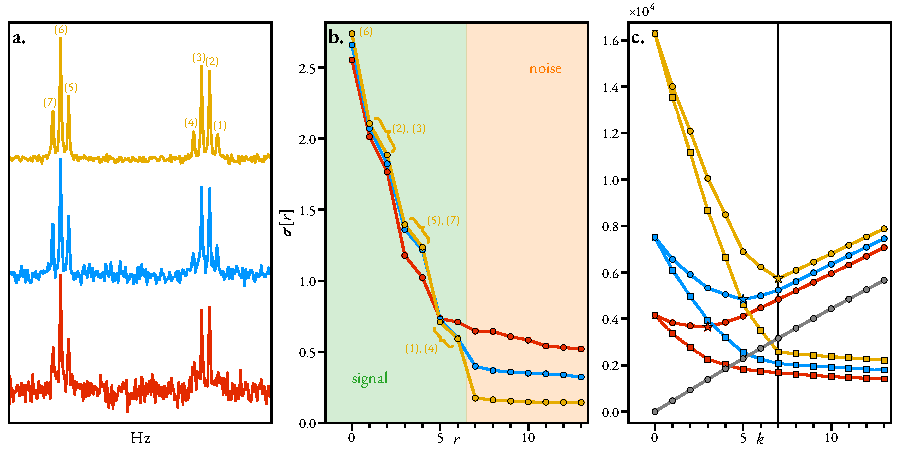
\includegraphics{mdl/mdl.pdf}
    \caption[
        An visualisation of the behaviour of the \acs{MDL} for three different
        \acsp{FID} comprising the same model, but with different noise variances.
    ]{
        An visualisation of the behaviour of the \acs{MDL} for three different
        \acsp{FID} comprising the same model, but with different noise
        variances. The model used to construct the \acp{FID} feature 7
        oscillators. The three \acsp{SNR} used were
        \qty{7}{\deci\bel} (red), \qty{12}{\deci\bel} (blue), and
        \qty{20}{\deci\bel} (yellow). The \acsp{FID} were generated with $\None
        = 256$.
        \textbf{a.} Spectra of the three \acsp{FID}.
        \textbf{b.} The values of the 14 most significant singular values
        associated with the Hankel matrix $\symbf{H}_{\symbf{Y}}$, with the
        pencil parameter $\Lone$ set to $\lfloor \nicefrac{\None}{3} \rfloor =
        85$).
        \textbf{c.} Square points with dotted lines: The negative log-likeliood
        \ac{MLE}, i.e. the first term of \eqref{eq:mdl}.
        Grey line: the penalty component of the \ac{MDL}, given by the second
        term in \eqref{eq:mdl}.
        Circular points with solid lines: the \ac{MDL}.
        Stars denote the minimum of the \ac{MDL} for a given \ac{FID}. The
        \qty{20}{\deci\bel}
        signal is correctly deemed to have a model order of 7, while the other
        two are underestimated (predicted models orders are 5 and 3 for the
        \qty{12}{\deci\bel} and \qty{7}{\deci\bel} \acsp{FID}, respectively).
    }
    \label{fig:mdl}
\end{figure}
Figure \ref{fig:mdl} illustrates the form of the \ac{MDL} for three signals
with equivalent underlying models, with $M=7$, and noise instances with
different variances. The first 14 singular values of $\symbf{H}_{\symbf{Y}}$
are plotted in panel b, where it can be seen that beyond the first 7, after
singular values accounting for signal components are accounted for, the
following singular values, associated with noise, decrease at a far slower
rate. The noise subspace for \acp{FID} with higher \acp{SNR} have singular
values which are (a) smaller in magnitude and (b) more consistent, such that
distinguishing the noise and signal subspaces is an easier task (cf. the
yellow line in panel b and the red line). As such, the \ac{MDL} is more likely
to provide a faithful estimate of the true number of components in the \ac{FID}
(panel c).

\note{Mention that multidimensional criteria are available, though not
implemented in this work.}

\section{\Acl{NLP} for NMR estimation}
\label{sec:nlp}
Attention now turns to the application of \acfi{NLP} in for \ac{FID}
estimation, which in this work accepts an initial guess of parameters from
the \ac{MPM}, $\symbf{\theta}^{(0)}$, and generates the final estimate,
$\bthstar$.

\subsection{An overview of \ac{NLP}}
\label{subsec:nlp-overview}
In an optimisation problem, the goal is to determine the minimum\footnote{
    In certain applications, the interest is actually in finding the maximum of
    a function. However, it is trivial to transform a maximisation problem into
    a minimisation problem by finding the minimum of negative of the function.
}
of a function $\Fth: \mathbb{R}^n \rightarrow \mathbb{R}, n \in \mathbb{N}$, often
called the \emph{cost function} or \emph{fidelity}.
This is typically with the goal of determining the argument $\bthstar$ at
which the optimum is found:
\begin{equation}
    \bthstar = \argmin_{\bth \in \mathbb{R}^n} \Fth.
    \label{eq:minF}
\end{equation}
The above problem is \emph{unconstrained}, as there are no limitations that the
parameter vector is subjected to. Unless $\Fth$ has particular properties, such
as convexity\footnote{
    A convex function is one such that a line segment through any two points of
    the function lies above it.
}, it is generally only possible to determine a \emph{local minimum},
rather than a \emph{global minimum}. $\bthstar$ is a local
minimiser of $\Fth$ if there is a \emph{neighbourhood} $V \ni \bthstar$ for which
\begin{equation}
    \Fthstar \leq \Fth\ \forall \bth \in V.
  \label{def:local-minimiser}
\end{equation}
$V \subset \mathbb{R}^n$ is such that one can move some amount in any direction
away from $\bthstar$ and still be in $V$.

Key to \ac{NLP} are the \emph{necessary conditions}, which define whether a
given vector $\bth$ is a local minimum of$\mathcal{F}$.
The \emph{first necessary condition} states
that if $\Fth$ is continuously differentiable, and $\bthstar$ is a local extremum of
$\Fth$, then the gradient vector $\bdgthstar \coloneq \nabla \Fthstar$ is the
zero vector:
\begin{equation}
    \bdgthstar = \symbf{0} \in \mathbb{R}^n
\end{equation}
The \emph{second necessary condition} subsequently states that
if $\Fth$ and $\bdgth$ are continuously differentiable, and $\bthstar$ is a
local minimiser of $\Fth$, then the Hessian matrix $\bdHthstar \coloneq
\nabla^2 \Fthstar$ is positive semidefinite, i.e.
\begin{equation}
  \symbf{v}^{\mathrm{T}} \bdHthstar \symbf{v} \geq 0\ \forall \symbf{v} \in \mathbb{R}^n.
\end{equation}
Furthermore, it is a \emph{unique} local minimiser if the \emph{second-order
sufficient condition} is also satisfied, i.e. that the Hessian is positive
definite:
\begin{equation}
    \symbf{v}^{\mathrm{T}} \bdHthstar \symbf{v} > 0\ \forall \symbf{v} \in \mathbb{R}^n.
\end{equation}

A plethora of approaches have been established to determine local minima of
scalar functions. One of the better-known strategies is \emph{Newton's method},
in which a quadratic approximation of the fidelity is considered.
For a given iteration $k \in \mathbb{N}_0$, the fidelity is approximated using
\begin{equation}
    \FQth =
        \Fthk +
        \symbf{h}\T \bdgthk +
        \tfrac{1}{2} \symbf{h}^{\mathrm{T}} \bdHthk \symbf{h},
    \label{eq:quad-approx}
\end{equation}
where $\symbf{h} = \bth - \bthk$.  An updated prediction of the parameter
vector is derived by finding the minimum of this quadratic approximation:
\begin{gather}
    \frac{\partial \Fth}{\partial \symbf{h}} =
        \bdgthk + \bdHthk \symbf{h} \notag\\
    \implies 0 = \bdgthk + \bdHthk \left(\bthkplusone - \bthk\right) \notag\\
    \therefore\ \bthkplusone =
        \bthk - \bdHthk^{-1}
        \bdgthk.\label{eq:newton-update}
\end{gather}
This process is repeated, until the convergence criterion as been met:
\begin{equation}
    \left\lVert \bdgthk \right\rVert \leq \epsilon.
\end{equation}
The threshold $\epsilon > 0$, can be tuned based on the desired accuracy of the
result, and is usually several order of magnitude less than $1$.
\Cref{eq:newton-update} tends not to be used as the update formula in real
optimisation problems. One of the major downsides of the Newton update is the
possibility that is not a minimising update if the Hessian is not positive
definite. Two primary strategies have emerged which are typically used instead:
\begin{itemize}
    \item \emph{Line search methods}\cite[Chapter 3]{Nocedal2006} determine an
        appropriate direction $\symbf{p}^{(k)}$ along which the updated
        parameter vector is sourced.  After this, an appropriate step length
        $\alpha^{(k)}$ is determined\,---\,typically in an efficient, though not
        optimal manner; abiding by the \emph{Wolfe conditions} is a common
        approach\,---\,leading to $\bthkplusone = \bthk -
        \alpha^{(k)}\symbf{p}^{(k)}$.
    \item \emph{Trust region methods}\cite[Chapter 4]{Nocedal2006} define a
        radius $\Updelta^{(k)} > 0$, and determine the minimum of
        \cref{eq:quad-approx} subject to the constraint that
        $\left\lVert\symbf{h}\right\rVert \leq \Updelta^{(k)}$.
\end{itemize}
A trust region method is applied in this work, and as such further
consideration of it will now be made.

\subsubsection{Trust Region Methods}

\begin{algorithm}
    \caption[
        Nonlinear programming routine employed in \acs{EsPy}.
    ]
    {
        Nonlinear programming routine employed in \acs{EsPy}. This makes use of
        Algorithms 4.1 \& 7.2 in \cite{Nocedal2006}, with a extra check
        inserted to deal with any negative-amplitude oscillators which may be
        generated as the routine evolves.
    }
    \label{alg:nlp}
    \begin{algorithmic}[1]
        \Procedure {NLP}{$\bY \in \mathbb{C}^{\None \times \cdots \times \ND}, \bthzero \in \mathbb{R}^{2(D + 1)M}$}
            \State $\trustradius{0} \gets \nicefrac{1}{10} \left\lVert \bdgthzeroY \right\rVert$;
            \State $\trmax \gets 16 \trustradius{0}$;
            \For {$k = 0, 1, \cdots $}
            \State $\symbf{p}^{(k)} \gets \textsc{SteihaugToint}\left(\symbf{Y}, \symbf{\theta}^{(k)}, \trustradius{k}\right)$;
                \Comment{See \cref{alg:steihaug-toint}}
                \State $\rho^{(k)} \gets
                    \frac
                        {\Fphithk - \Fphithkpk}
                        {\FphiQthk - \FphiQthkpk}$;
                \If {$\rho_k < \nicefrac{1}{4}$}
                \label{state:decrease-tr-start}
                \State $\trustradius{k+1} \gets \nicefrac{1}{4} \trustradius{k}$;
                    \label{state:decrease-tr-end}
                    \ElsIf {$\rho_k > \nicefrac{3}{4}$ \textbf{ and } $\left\lVert \symbf{p}^{(k)} \right\rVert = \trustradius{k}$}
                \label{state:increase-tr-start}
                \State $\trustradius{k+1} \gets \min\left(2 \trustradius{k}, \trmax\right)$;
                    \label{state:increase-tr-end}
                \Else
                \State $\trustradius{k+1} \gets \trustradius{k}$;
                \EndIf
                \If{$\rho^{(k)} > \nicefrac{3}{20}$}
                \label{state:large-rho-start}
                    \State $\bthkplusone \gets \bthk + \symbf{p}^{(k)}$;
                    \label{state:large-rho-end}
                \Else
                \label{state:small-rho-start}
                    \State $\symbf{\theta}^{(k+1)} \gets \symbf{\theta}^{(k)}$;
                    \label{state:small-rho-end}
                \EndIf
                \If{$k \bmod 25 = 0 \textbf{ and } \symbf{\theta}^{(k+1)}$ contains negative amplitudes}\label{state:neg-amp-start}
                    \State $\symbf{\theta}^{(0)} \gets \symbf{\theta}^{(k+1)}$ with negative-amplitude oscillators removed;
                    \State $\symbf{\theta}^{(*)}, \symbf{\epsilon}^{(*)} \gets \operatorname{NLP}\left(\symbf{Y}, \symbf{\theta}^{(0)}\right)$;
                \EndIf\label{state:neg-amp-end}
                \If{$\left\lVert \bdgthkplusone \right\rVert < \num[print-unity-mantissa=false]{1e-8}$}
                    \State \textbf{break};
                \EndIf
            \EndFor
            \State $\symbf{\theta}^{(*)} \gets \symbf{\theta}^{(k+1)}$
            \State $\symbf{\epsilon}^{(*)} \gets
                \sqrt{
                    \frac
                    {
                        \Fthstar \diag \left(
                            \left[\bdHthstar\right]^{-1}
                        \right)
                    }
                    {(\None \cdots \ND) - 1}
                }$
            \State \textbf{return} $\symbf{\theta}^{(*)}, \symbf{\epsilon}^{(*)}$;
        \EndProcedure
    \end{algorithmic}
\end{algorithm}

The structure of a typical trust region method is presented in
\cref{alg:nlp} (ignoring \crefrange{state:neg-amp-start}{state:neg-amp-end}, which is a custom addition,
see \cref{subsec:phase-variance}). An initial radius for the trust region
$\trustradius{0}$ is defined, along with a maximum permitted radius
$\trmax$, to ensure that excessively adventurous steps do not take place.
For each iteration $k$, a solution to the following sub-problem is sought:
\begin{equation}
    \begin{split}
        \bthkplusone = \argmin_{\bp \in \mathbb{R}^{n}}
            \Fthk +
            (\bthk + \bp)\T \bdgthk +
            \tfrac{1}{2} (\bthk + \bp)\T \bdHthk (\bthk + \bp) \\
        \text{subject to } \left \lVert \bp \right \rVert \leq \trustradius{k}.
    \end{split}
\end{equation}
This sub-problem is not usually minimised exactly, but instead an efficient
means of determining a sufficiently update is used.
Common approaches include computing the Cauchy point, the Dogleg
method, and a truncated conjugate-gradient
approach commonly called the \ac{ST} method\cite[Chapter 7]{Nocedal2006}.
The latter is employed in this work (see \cref{alg:steihaug-toint} and
\cref{lst:tr}). In the \ac{ST} approach, iterates of the conjugate-gradient
method\cite[Chapter 5]{Nocedal2006} are used, until either they go beyond the
trust region, or negative curvature is discovered.

Once a provisional update $\bthkplusone \coloneq \bth + \bpk$ is determined, a
metric is considered which indicates how effectively the quadratic estimate at
the proposed update $\bthkplusone = \bthk
+ \bpk$ agrees with the true value of the fidelity at this point:
\begin{equation}
    \rho^{(k)} = \frac
        {\Fthk - \Fthkpk}
        {\FQthk - \FQthkpk}.
\end{equation}
$\rho^{(k)}$ is the ratio between the actual reduction of the fidelity caused
by taking the proposed step, and the predicted reduction based on the quadratic
model. If $\rho^{(k)}$ is sufficiently close to $1$, the quadratic model being
used to generate new iterates is deemed to be acting well enough to warrant
accepting the proposed update
(\crefrange{state:large-rho-start}{state:large-rho-end}).
Furthermore, if $\rho^{(k)}$ is particularly close to 1, and the proposed
update is at the boundary of the trust radius, it is appropriate to enlarge the
radius of the trust region for the next iteration in an attempt to increase the
rate of convergence
(\crefrange{state:increase-tr-start}{state:increase-tr-end}).
On the other hand, a small value of $\rho^{(k)}$ implies that the
quadratic model reflects the true fidelity poorly, such that the proposed
update should be rejected
(\crefrange{state:small-rho-start}{state:small-rho-end}).
As well as this, the trust region's radius should be
decreased such that the model is more likely to behave faithfully
(\crefrange{state:decrease-tr-start}{state:decrease-tr-end}). The exact
thresholds which dictate whether to accept an update, and whether to adjust the
trust region radius are customisable. The hard-coded numerical values found in
\cref{alg:nlp} are the values used for the results acquired in this work.

\subsection{Non-linear programming applied to FID estimation}
\begin{remark}
    \label{rem:norm-data}
    Prior to estimating the dataset, it is normalised, such that the signal
    actually under consideration is $\nicefrac{\bY}{\lVert \bY \rVert}$.
    To make the result reflect the actual dataset, the final amplitudes $\bdastar$
    are multiplied by $\lVert \symbf{Y} \rVert$.
\end{remark}
Focussing now on the problem of FID estimation, the fidelity $\FthY
: \mathbb{C}^{\None \times \cdots \times \ND} \times
\mathbb{R}^{2(1 + D)M} \rightarrow \mathbb{R}$ is given by
\begin{equation}
    \FthY = \left \lVert \bY - \bXth \right \rVert^2.
    \label{eq:fidelity}
\end{equation}
The elements of the gradient vector $\bdgthY \in \mathbb{R}^{2(1+D)M}$ and
the Hessian matrix $\bdHthY \in \mathbb{R}^{2(1+D)M \times 2(1+D)M}$ are then
derived by taking the first and second partial derivatives of the fidelity with
respect to the elements in $\bth$, respectively:
\begin{subequations}
    \begin{gather}
        g_i = -2 \Re
                \left\langle
                    \left(\bY - \bX\right),
                    \frac{\partial \bX}{\partial \theta_i}
                \right\rangle,
        \label{eq:grad} \\
        h_{i,j} = 2 \Re
            \biggl(
                \underbrace{
                    \left\langle
                        \frac{\partial \bX}{\partial \theta_i},
                        \frac{\partial \bX}{\partial \theta_j}
                    \right\rangle
                }_{\circled{1}}
                -
                \underbrace{
                    \left\langle
                        \left(\bY - \bX\right),
                        \frac{\partial^2 \bX}{\partial \theta_i \partial \theta_j}
                    \right\rangle
                }_{\circled{2}}
            \biggl).
            \label{eq:hess}
    \end{gather}
    \label{eq:fidelity-grad-hess}
\end{subequations}
$\forall i,j \in \lbrace 1, \cdots, 2(1+D)M \rbrace$.
The complete set of first and second derivatives of a particular element of the
model $x \coloneq \xnonenD$, given by \cref{eq:x}, is as follows
$\forall m \in \lbrace 1, \cdots, M \rbrace$,
$\forall d, d^{\prime} \in \lbrace 1, \cdots, D \rbrace$:
\begin{subequations}
    \begin{gather}
        \xderiv{\theta_m} \equiv
            \xderiv{a_m} =
            \frac{x}{a_m},\\
        \xderiv{\theta_{m + M}} \equiv
            \xderiv{\phi_m} =
            \iu x,\\
        \xderiv{\theta_{m + (d + 1)M}} \equiv
            \xderiv{\fdm} =
            2 \pi \iu \Dtd \nd x,\\
        \xderiv{\theta_{m + (d + D + 1)M}} \equiv
            \xderiv{\etadm} =
            - \Dtd \nd x,\\
        \xderivtwosame{\theta_{m}} \equiv
            \xderivtwosame{a_m} =
            0,
            \label{eq:amp-second-deriv}\\
        \xderivtwodiff{\theta_{m}}{\theta_{m + M}} \equiv
            \xderivtwodiff{a_m}{\phi_m} =
            \frac{\iu x}{a_m},\\
        \xderivtwodiff{\theta_{m}}{\theta_{m + (d + 1)M}} \equiv
            \xderivtwodiff{a_m^{\vphantom{(d)}}}{\fdm} =
            \frac{2 \pi \iu \Dtd \nd x}{a_m},\\
        \xderivtwodiff{\theta_{m}}{\theta_{m + (d + D + 1)M}} \equiv
            \xderivtwodiff{a_m^{\vphantom{(d)}}}{\etadm} =
            \frac{-\Dtd \nd x}{a_m},\\
        \xderivtwosame{\theta_{m + M}} \equiv
            \xderivtwosame{\phi_m} =
            -x,\\
        \xderivtwodiff{\theta_{m + M}}{\theta_{m + (d + 1)M}} \equiv
            \xderivtwodiff{\phi_m^{\vphantom{(d)}}}{\fdm} =
            -2 \pi \Dtd \nd x,\\
        \xderivtwodiff{\theta_{m + M}}{\theta_{m + (d + D + 1)M}} \equiv
            \xderivtwodiff{\phi_m^{\vphantom{(d)}}}{\etadm} =
            -\iu \Dtd \nd x,\\
        \xderivtwodiff{\theta_{m + (d + 1)M}}{\theta_{m + (d^{\prime} + 1)M}} \equiv
            \xderivtwodiff{\fdm}{\fdmp} =
            -4\pi^2 \left(\Dtd \nd \right) \left(\Dtdp \ndp \right) x,\\
        \xderivtwodiff{\theta_{m + (d + 1)M}}{\theta_{m + (d^{\prime} + D + 1)M}} \equiv
            \xderivtwodiff{\fdm}{\etadmp} =
            -2 \pi \iu \left(\Dtd \nd \right) \left(\Dtdp \ndp \right) x,\\
        \xderivtwodiff{\theta_{m + (d + D + 1)M}}{\theta_{m + (d^{\prime} + D + 1)M}} \equiv
            \xderivtwodiff{\etadm}{\etadmp} =
            \left(\Dtd \nd \right) \left(\Dtdp \ndp \right) x,\\
        \xderivtwodiff{\theta_{i}}{\theta_{j}} =
            \xderivtwodiff{\theta_{j}}{\theta_{i}},
            \label{eq:symmetric-second-derivs}\\
        \xderivtwodiff{\theta_{i}}{\theta_{j}} = 0\ \text{ if not specified above.}
        \label{eq:zero-second-deriv}
    \end{gather}
\end{subequations}
\Cref{eq:zero-second-deriv} indicates that any second derivative
with respect to two parameters which do not belong to the same oscillator will
always be $0$. This, along with the symmetrical nature of the second derivatives, see
\cref{eq:symmetric-second-derivs}, drastically reduces the required
number of second derivatives to compute, from $4 (1 + D)^2 M^2$ per data-point
to  $(1+D)\left(3 + 2D\right)M$. Finally, \cref{eq:amp-second-deriv}
indicates that another $M$ second derivatives do not need to be computed. See
\cref{tab:number-of-derivatives} for the total number of derivatives that need
to be computed for signals with different numbers of dimensions.
\begin{table}
    \begin{center}
        \begin{tabular}{ c c c }
            \toprule
            dimensions &
                \# 1\textsuperscript{st} derivatives &
                \# 2\textsuperscript{nd} derivatives\\
            \midrule
            $1$ & $4M\None$ & $9M\None$\\
            $2$ & $6M\None\Ntwo$ & $20M\None\Ntwo$\\
            $3$ & $8M\None\Ntwo\Nthree$ & $35M\None\Ntwo\Nthree$\\
            $D$ &  $2(1 + D)M \None \cdots \ND$ &  $((1 + D)(2(1 + D) + 1) - 1)M \None\cdots\ND$\\
            \bottomrule
        \end{tabular}
    \end{center}
    \caption{
        The number of first and second derivatives that are necessary to
        compute both the gradient vector and Hessian matrix of the fidelity for
        1- 2- and 3-dimensional datasets, as well as a general $D$-dimensional
        dataset.
    }
    \label{tab:number-of-derivatives}
\end{table}

\subsection{Approximating the Hessian}
Despite many of the model second derivatives being $0$, computation of those
that are not zero, and subsequently using these the form the Hessian matrix, is
often the most computationally expensive part of the optimisation. There are a
large number of optimisation problems where this is the case, and as such
there is considerable precedent for improving the efficiency of optimisation
algorithms by generating approximations of the Hessian which are less expensive.
Examples include the \ac{GN} method and \ac{LM} algorithm,
which are specifically for residual sum-of-squares problems\cite[Chapter
10]{Nocedal2006}, as well as quasi-Newton methods such as the BFGS
method\cite[Chapter 6]{Nocedal2006}.

The \ac{GN} and \ac{LM} approaches replace the true Hessian matrix at each
iteration with the following expression:
\begin{equation}
    h_{i,j} \approx 2 \Re
        \left\langle
            \frac{\partial \bX}{\partial \theta_i},
            \frac{\partial \bX}{\partial \theta_j}
        \right\rangle,
    \label{eq:hess-approx}
\end{equation}
i.e. term \circled{2} in \cref{eq:hess} involving the second derivatives is
neglected. All that needs to be generated is the Jacobian
$\symbf{J} = \nicefrac{\partial \bX}{\partial \bth}$. This often
brings a very large reduction in the computational cost, as no extra
derivatives need to be computed for the Hessian at all, since the Jacobian is
already required for generating the gradient vector.
In situations where the residuals between the data and model are small, term
\circled{1} will tend to dominate term \circled{2}, and as such these methods
often enjoy a convergence rate close to that of Newton's method when close to
local minima. Despite this, by invoking this approximation, the rate of
convergence, i.e. the number of iterations required to reach $\bthstar$, tends
to be adversely affected. See \cref{subsec:optim-vis} for an example of
this phenomenon.

\subsection{Estimation Errors}
\label{subsec:errors}
The vector of standard errors associated with the \ac{NLP} routine is related
to the \emph{observed Fisher information matrix} at convergence\cite[Section
2.7]{Pawitan2001}:
\begin{equation}
    \symbf{\epsilon}\left(\bthstar\right) = \sqrt{\diag\left(\symbf{I}\left( \bthstar \right)^{-1}\right)},
\end{equation}
where the observed Fisher Information matrix contains the negative partial second
derivatives of the log-likelihood with respect to $\bth$:
\begin{equation}
    \symbf{I}\left(\bth\right)_{i, j} =
        -\frac
        {\partial^2 \ell \left( \bdthY \right)}
        {\partial \theta_i \partial \theta_j}.
\end{equation}
Recalling the form of the log-likelihood given by \cref{eq:log-likeihood},
the elements of $\symbf{I}\left(\bth\right)$ are
\begin{equation}
    \symbf{I}\left(\bth\right)_{i, j} =
        -\frac{1}{\sigma^2}
        \Re
        \biggl(
            \left\langle
                \frac{\partial \bX}{\partial \theta_i},
                \frac{\partial \bX}{\partial \theta_j}
            \right\rangle
            -
            \left\langle
                \left(\bY - \bX\right),
                \frac{\partial^2 \bX}{\partial \theta_i \partial \theta_j}
            \right\rangle
        \biggl),
\end{equation}
which very closely resembles the Hessian of $\bth$:
\begin{equation}
    \symbf{I}\left(\bth\right)_{i,j} =
        \frac{1}{2 \sigma^2} \left(
            \bdHth_{i,j}
        \right).
\end{equation}
The standard errors therefore take the form
\begin{equation}
    \symbf{\epsilon}\left(\bthstar\right) =
        \sqrt{
            2\sigma^2 \diag \left(
                \bdHthstar^{-1}
            \right)
        }.
\end{equation}
Considering that the mean and variance of the noise $\bW$ are $0$ and $2\sigma^2$, respectively:
\begin{equation}
    2 \sigma^2 = \frac{1}{\mathfrak{N} - 1}
    \left\lVert \bW \right\rVert^2 =
    \frac{1}{\mathfrak{N} - 1} \left \lVert
        \bY - \bXthstar
    \right \rVert^2,
\end{equation}
so that finally a useable expression for the standard errors is arrived at:
\begin{equation}
    \symbf{\epsilon}\left(\bthstar\right) =
        \sqrt{
            \frac
            {
                \Fthstar \diag \left(
                    \left[\bdHthstar\right]^{-1}
                \right)
            }
            {\mathfrak{N} - 1}
        }
\end{equation}

\subsection{Visualisation of a simple example}
\label{subsec:optim-vis}
\begin{figure}
    \centering
    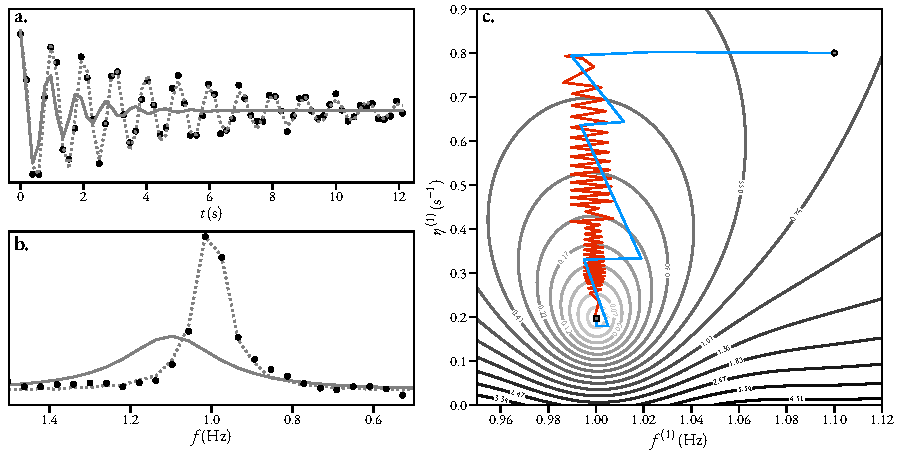
\includegraphics{optimisation_visualisation/optimisation_visualisation.pdf}
    \caption[
        A visualisation of the trajectory of a 2-parameter optimisation
        involving a simulated \acs{FID} comprising a single resonance.
    ]
    {
        A visualisation of the trajectory of a 2-parameter optimisation
        involving a simulated \acs{FID} comprising a single resonance.
        \textbf{a.} \& \textbf{b.} Representations of the signal in
        the time domain and Fourier domain, respectively.
        Black dots: the signal to be estimated $\bY$.
        Solid grey line: the model generated
        using the initial guess $\bX \left( \bthzero \right)$.
        Dotted grey line: the model generated using the optimised result, $\bX
        \left( \bthstar \right)$.
        \textbf{c.} A contour plot of the fidelity.
        Blue line: the trajectory of the parameter vector with the true
        Hessian matrix used in computing each update.
        Red line: the analogous trajectory using the Hessian approximation
        in place of the true Hessian.
    }
    \label{fig:optim-vis}
\end{figure}
\Cref{fig:optim-vis} provides a visualisation of numerical optimisation
applied on a simulated \ac{FID} comprising a single resonance.
The FID was constructed using \cref{eq:general-fid} with $D=1$, $M=1$,
$\None = 64$, $\fswone = \qty{5.2}{\hertz}$ ($\Dtone \approx
\qty{0.192}{\per\second}$), and $\foffone = \qty{0}{\hertz}$.
The resonance was parameterised by $\bth \in \mathbb{R}^4$ comprising $a=1$,
$\phi=\qty{0}{\radian}$, $\fone=\qty{1}{\hertz}$, $\etaone=\qty{0.2}{\per\second}$.
White Gaussian noise was added to the FID to give it \iac{SNR} of approximately
\qty{10}{\deci\bel}. As the visualisation of 5D space is beyond the scope of
this work, only two parameters, the frequency and damping factor were optimised
from an initial guess, with the amplitude and phase being fixed to their true
values. The initial guess comprised a frequency of \qty{1.1}{\hertz}, and a
damping factor of \qty{0.8}{\per\second}, with the solid grey lines in panels a
\& b denoting the model generated using the initial guess in the time- and
Fourier-domains, respectively. $\bthzero$ was subjected to \ac{NLP} twice. In
the first instance, the exact Hessian matrix, given by \cref{eq:hess} was used
in order to compute each update step, while in the second the Hessian
approximation given by \cref{eq:hess-approx} was used. The initial
radius of the trust region was set to $\nicefrac{1}{10}$ of the gradient norm
($\approx 0.3$), which has a precedent in the literature\cite{Gould2005}. The
trajectories of the parameter vector are denoted as coloured lines in panel c.
In both cases, the \ac{NLP} routine successfully generated a result $\bthstar$
in agreement with the true frequency and damping factor used to construct the
\ac{FID}. However, it is clear that using the true Hessian matrix (blue)
led to a far better rate of convergence compared with the
approximated analogue (red), which exhibited ``zig-zagging''. This phenomenon
is often seen in gradient descent methods, in which each update occurs in the
opposite direction to the gradient.
14 iterations were required to reach the
convergence criterion $\epsilon \leq \num[print-unity-mantissa=false]{1e-8}$
when the true Hessian was used, while 81 were required for the approximated
case. While an anecdotal example, this highlights that use of the true
Hessian matrix tends to allow a better rate of convergence. However, for
\acp{FID} comprising many signals and far more points, the approximated form
often requires a shorter time to converge overall, as the cost of computing the
second derivatives required for the true Hessian dominates.

\subsection{Phase Variance Minimisation}
\label{subsec:phase-variance}
\note{Re-write this section}
While numerical optimisation procedures can return estimates $\bthstar$ which
can achieve highly accurate reconstructions of the original \acs{FID} (i.e.
$\bY$ and  $\bXthstar$ are in close agreement), the estimate won't
necessarily provide a faithful description of the physical phenomenon that has
given rise to the data. For the purposes of \ac{FID} estimation, the goal is to
ensure that each signal contributing to the \ac{FID} is described by a
single oscillator in the model. In scenarios where the model order $M$ used is
greater than the true number of resonances, over-fitting of the data will
occur, leading to spurious features in the estimation result, such as single
resonances being fit by multiple oscillators and/or noise components being fit.
To overcome this problem, it is desirable to include known information about
the signal into the optimisation routine as a means of guiding the parameter
vector to a more appropriate final value. One particular means of achieving
this which has been to found to be effective is the incorporation of the
variance of oscillator phases into the fidelity, such that it becomes
\begin{equation}
    \FphithY = \left \lVert \bY - \bXth \right \rVert^2 + \circvar,
    \label{eq:fidelity-phasevar}
\end{equation}
where $\circvar$ is the \emph{circular variance} of the oscillator phases
(\textit{vide infra}).
\begin{remark}
    The inclusion of the phase variance into the fidelity is one of the
    motivating reasons for normalising the data prior to estimation (see
    \cref{rem:norm-data}). $\circvar$ is constrained to the interval $[0, 1]$.
    If the data were not normalised, it is likely that $\lVert \bY - \bX
    \rVert^2$ would dominate $\circvar$ in \cref{eq:fidelity-phasevar},
    such that the influence of the phase variance would be negligible.
\end{remark}
For the phase variance to act effectively, it is necessary to apply
phase-correction to the data prior to estimation, as the assumption that the
phases of all contributing resonances are equal is typically
valid.
\note{Mention phase-variation of multiplet peaks in experiments where
J-coupling evolves prior to acquisition? $T_2$ for example.}
The inclusion of phase variance has also been found to be effective at purging
excessive oscillators that may be present in the initial guess $\bthzero$,
which be thought of in the following way:
\begin{enumerate}
    \item Assume that the initial guess contains more oscillators than the
        true number of resonances. In this circumstance, it is common to find
        that true resonances are fit with an acceptable oscillator, whilst
        extra oscillators exist with spurious phases on account of
        over-fitting.
    \item Unconstrained numerical optimisation is now run, with the fidelity
        given by \cref{eq:fidelity-phasevar}. The phase variance will
        force oscillators with phases that are significantly different to the
        majority of oscillators to drastically alter their phases to match
        them. For some/all of these oscillators, it may be the case that the
        optimiser drives these to acquire a negative amplitude, such that they
        act as if they have a phase of $\pi$ while ensuring that $\circvar$ is
        small.
    \item This provides a criterion for detecting oscillators which are likely
        to be excessive. Such oscillators can be purged from $\bth$ by
        periodically checking whether any amplitudes (i.e. $\bth[:M]$) have
        become negative, purging these, and re-starting the optimisation.
    \item The numerical optimisation routine is re-started each time
        oscillators are purged. Termination is achieved once the routine
        converges and no negative-amplitude oscillators exist in $\bth$.
\end{enumerate}

\subsubsection{Circular Variance}
Oscillator phases are an example of a \emph{circular variable}, in that all
phases are wrapped within an interval of width $2 \pi$. Given an unconstrained
(unwrapped) phase $\widetilde{\phi} \in \mathbb{R}$, the corresponding wrapped
phase $\phi \in \left( -\pi, \pi \right]$ is given by
\begin{equation}
    \phi = \left(\left(\widetilde{\phi} + \pi\right) \bmod 2 \pi\right) - \pi.
    \label{eq:phase_wrap}
\end{equation}
This makes the conventional (linear)
definition of variance, given by
\begin{subequations}
    \begin{gather}
        \Var_{\shortmid}\hspace*{-3pt}\left(\symbf{\phi}\right) =
            \frac{1}{M} \sum_{m=1}^{M} \left(\phi_m - \mu\left(\symbf{\phi}\right)\right)^2, \\
        \mu\left(\symbf{\phi}\right) = \frac{1}{M} \sum_{m} \phi_m,
    \end{gather}
\end{subequations}
unsuitable for phases. Consider as a simple example a scenario
where there are two oscillators with phases $\widetilde{\bdphi} = \left[ \pi +
\delta\:\:\pi - \delta \right]\T$ for some small $\delta$.
The phase variance is expected to be small as these two phases are similar.
However, with the inclusion of wrapping through application of
\cref{eq:phase_wrap}, these phases would actually be set to $\bdphi = \left[
    -\pi
+ \delta\:\:\pi - \delta \right]\T$, and the conventional definition of phase
variance would be large. It is therefore apparent that a definition of variance
which accounts for the periodicity of the phases is needed. The \emph{circular
variance} is given by\cite[Chapter 3]{Fisher1993}
\begin{subequations}
    \begin{gather}
        [0, 1] \ni \circvar = 1 - \frac{R}{M},\\
        R = \sqrt{c_{\Sigma}^2 + s_{\Sigma}^2}, \\
        c_{\Sigma} = \sum_{m} \cos \phi_m, \\
        s_{\Sigma} = \sum_{m} \sin \phi_m.
    \end{gather}
\end{subequations}
$R$ is the length of the resultant vector produced by summing $M$ unit vectors
with the angles given by $\bdphi$. In the case that all the vectors have the
same angle, $R=M$, leading to the variance being $0$ as expected. At the other
extreme, with $M$ vectors uniformly separated about the unit circle (with an
angle $\nicefrac{2 \pi}{M - 1}$ between all pairs of adjacent vectors), the
vectors will perfectly cancel, leading to $R=0$. In this case, the maximum
variance of $1$ is obtained.

The first and second derivatives of the circular variance are required for
the computation of the gradient vector and Hessian matrix. These are given by
\begin{subequations}
    \begin{gather}
        \frac{\partial \circvar}{\partial \theta_i} =
        \begin{cases}
            \frac{1}{RM}
            \left(
                c_{\Sigma} \sin \phi_{i-M} -
                s_{\Sigma} \cos \phi_{i-M}
            \right) & M \leq i < 2M\\
            0 & \text{otherwise}
        \end{cases}\\
        \frac{\partial^2 \circvar}{\partial \theta_i \partial \theta_j} =
        \begin{cases}
            \begin{split}
                \tfrac{1}{RM}\left[
                    \tfrac{1}{R^2}
                    \left(c_{\Sigma} \sin \phi_{i-M}  - s_{\Sigma} \cos \phi_{i-M} \right)^2 \right. \\
                    \left. + c_{\Sigma} \cos \phi_{i-M} + s_{\Sigma} \sin \phi_{i-M}
                    - 1
                \vphantom{\tfrac{1}{RM}}\right]
            \end{split}
            & M \leq i, j < 2M, i = j\\
            \begin{split}
                \tfrac{1}{RM}\left[
                    \tfrac{1}{R^2}
                    \left(c_{\Sigma} \sin \phi_{i-M} - s_{\Sigma} \cos \phi_{i-M} \right) \right.\\
                    \times \left(c_{\Sigma} \sin \phi_{j-M} - s_{\Sigma} \cos \phi_{j-M} \right) \\
                    \left. - \cos\left( \phi_{i-M} - \phi_{j-M} \right)
                    \vphantom{\tfrac{1}{R^2}}
                \right]
            \end{split}
            & M \leq i, j < 2M, i \neq j\\
            0 & \text{otherwise}
        \end{cases}
    \end{gather}
\end{subequations}



\section{Profiling the Method}
\label{sec:profiling}
The routine described for \ac{FID} estimation involves operations which can be
computationally demanding, with the burden on resources
increasing with the number of points in the \ac{FID}, as well as the number of
oscillators in the model. This is the case both in terms of the amount of work
done by the \ac{CPU}, and the amount of \ac{RAM} needed to store all the
required data as the routine runs. For the matrix pencil methods, the most
demanding aspect is performing \ac{SVD}, while for \ac{NLP}, it
is generation of the Hessian matrix for each iteration. Detailed accounts of the
computational complexity of the \ac{MPM} and \ac{MMEMPM} have been
presented~\cite{Hua1992,Chen2007}.  However, it is useful to consider what the
actual run times of these routines are on a modern computer; a lot of
accounts on these are from decades before this work, and so the
run time will have decreased considerably thanks to
improvements in processing power. As an example, the account by Pines a
co-workers from 1997 outlining the \ac{ITMPM} states that a signal comprising
$1024$ points would take about
\qty{4.5}{\minute} to be processed by the \ac{MDL} and \ac{MPM}, using a
\qty{100}{\mega\hertz} \ac{CPU}~\cite{Lin1997}. On the system used for all
results generated for this work (see \cref{rem:workstation}) an
equivalent computation takes about \qty{100}{\milli\second}.

To derive the results presented in this section, \Python\ implementations of
the aforementioned parts of the estimation routine were run, with software used
to assess both the line-by-line execution times~\cite{LineProf}, and the
time-dependent \ac{RAM} usage~\cite{MemProf}.
\begin{remark}
    \label{rem:workstation}
    All results presented in this work were acquired using a workstation
    featuring a Intel\textregistered\ Core\texttrademark\ i9-10900X \ac{CPU} @
    \qty{3.7}{\giga\hertz}, and \qty{32}{\gibi\byte} of \ac{RAM}.
\end{remark}

\subsection{The \acs{MPM} and \acs{MMEMPM}}
\label{subsec:mpm-profiling}
\begin{figure}
    \centering
    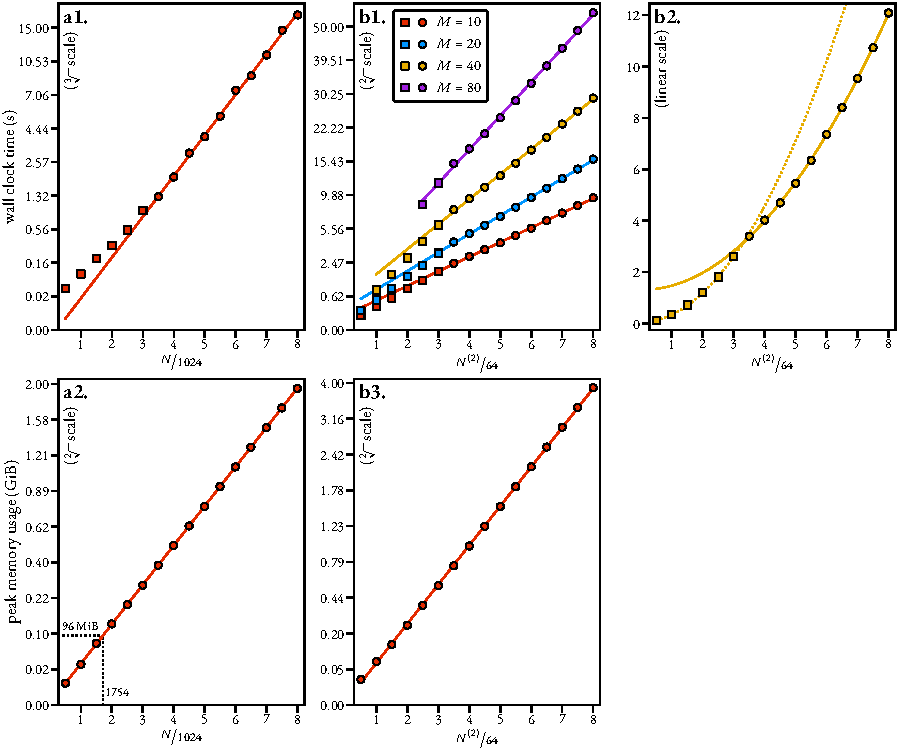
\includegraphics{mpm_profiling/mpm_profiling.pdf}
    \caption[
        The run time and peak memory consumption of
        the \acs{MPM} and \acs{MMEMPM}
        for \acsp{FID} with differing numbers of
        datapoints and constituent signals.
    ]
    {
        The run time and peak memory consumption of
        the \acs{MPM} and \acs{MMEMPM}
        for \acsp{FID} with differing numbers of
        datapoints and constituent signals.
        The \acp{FID} that were used to acquire these results are described in
        the main text.
        \textbf{a1.} The amount of time required to compute the \ac{MPM}, as a
        function of number of points. Also plotted is a cubic fit of the
        circular points.
        \textbf{a2.} Peak memory consumption in performing the \ac{MPM} as a
        function of the number of points.
        \textbf{b1.} The run time to compute the \ac{MMEMPM} of
        \acp{FID} with $\None = 64$, and variable $\Ntwo$ and $M$. Circular
        points have been fitted to quadratic functions.
        \textbf{b2.} The time required to compute the \ac{SVD} of $\EY$ for the
        $M=40$ \acp{FID}. The solid line is a quadratic fit of the circular
        points, while the dashed line is a quadratic fit of the square points.
        \textbf{b3.} Peak memory consumption in performing the \ac{MMEMPM} for
        the $M=40$ \acp{FID}.
    }
    \label{fig:mpm-profiling}
\end{figure}

A series of synthetic \ac{1D} \acp{FID} were constructed, comprising $10$ evenly-spaced
signals, with a
variable number of time-points $N \in \lbrace 512k : k \in \lbrace 1, 2, \cdots, 16 \rbrace \rbrace$.
For each \ac{FID}, the \ac{MPM} routine outlined in \cref{lst:mpm} was
performed 5 times.
The mean time to perform the \ac{MPM} across the 5 runs is plotted as a function
of $N$ in \cref{fig:mpm-profiling}.a1, where it can be seen that for
the larger values of $N$ considered, the \ac{MPM} is computed in approximately
$\mathcal{O}({N}^3)$ time;
a fit of a cubic function of the form $aN^3 + b$ to the data satisfying $7 \leq
k \leq 16$ is plotted to highlight this.
The cubic dependence is realised since the rate-limiting step of the
\ac{MPM} is \ac{SVD} of $\Hy$, whose size is to a very good approximation
$\tfrac{2N}{3} \times \tfrac{N}{3}$\footnote{
    \label{fn:svd-complexity}
    The time complexity for the \ac{SVD} of generic a $m \times n$ matrix is
    $\mathcal{O}(\operatorname{min}(m, n)^2 \cdot \operatorname{max}(m, n))$,
    while the space complexity is $\mathcal{O}(mn)$.
}. For smaller values of $N$, a deviation
away from a cubic relationship is observed.
This arises because the computation of the complex amplitudes using
\cref{eq:complex-amplitudes} has a comparatively significant run time
relative to \ac{SVD} in the low-$N$ regime;
for a $512$ point signal, \ac{SVD} of $\Hy$ took up roughly 80\% of the
complete run time, while the computation of the complex amplitudes took up
roughly 20\%. For a 8192 point signal, these percentages had changed to
$>\!\!99\%$ and $<\!\!1\%$, respectively.

The \ac{MPM} was run once more on each generated \ac{FID} in order to assess
the effect of $N$ on the space complexity.
The peak \ac{RAM} consumption is plotted in \cref{fig:mpm-profiling}.a2.
A clear quadratic dependence on consumption is realised as function of $N$,
again in agreement with the expected space complexity of the
\ac{SVD}\footnoteref{fn:svd-complexity}.

A similar study was conducted for the consideration of the \ac{MMEMPM}. A
series of hypercomplex \ac{2D} \acp{FID} were simulated, all of which all
comprised $\None = 64$. The \acp{FID} possessed values of $\Ntwo \in \lbrace
32k : k \in \lbrace 1, \cdots, 16 \rbrace \rbrace$.
With the \ac{MPM}, since a complete \ac{SVD} of the matrix $\Hy$ is computed,
the model order is irrelevant in dictating the run time (at least when $M \ll
N$). This is not the case for the \ac{MMEMPM}; because the \Python
implementation used (\cref{lst:mmempm}) employs a truncated \ac{SVD} in order
to compute only the first $M$ components of $\EY$, the elected model order will
have an impact on run time.  Therefore, \acp{FID} with different model orders
were generated: $M \in \lbrace 10, 20, 40, 80 \rbrace$.

The \ac{MMEMPM} was repeated 5 times for each \ac{FID}, and the mean run
times for each $\Ntwo$ and $M$ considered is plotted in
\cref{fig:mpm-profiling}.b1.
Results are only presented in cases where the \ac{MMEMPM} was able to yield a
satisfactory estimation result in close agreement with the model used to
generate the \ac{FID}; for certain \acp{FID} with low
$\Ntwo$ and high $M$, appropriate estimation results could not be obtained as
the constituent signals were too poorly resolved.
While in the high-$N$ regime the \ac{MPM} has a cubic time dependence
on the number of points, the \ac{MMEMPM} can be seen to have an approximately
quadratic complexity regarding $\Ntwo$.
For all combinations of $\Ntwo$ and $M$,
the truncated \ac{SVD} was the most time consuming aspect of the routine,
however other steps have notable run times too. The \ac{MMEMPM} can be broken
down into the following 5 steps, with the relevant lines in \cref{lst:mmempm}
given:
\begin{enumerate}
    \item Construction of $\EY$. This involves building the Hankel matrices
        $\lbrace \symbf{H}_{\symbf{y},\none} : \none \in \lbrace 0, \cdots, 63
        \rbrace \rbrace$, assigning them to the
        correct locations in $\EY$, and finally converting  $\EY$ to a sparse
        matrix\footnote{
            Truncated \ac{SVD} is only available for sparse matrices in
            \textsc{NumPy}~\cite{svds}. Some experimenting was done to determine
            the most efficient means of generating $\EY$ in sparse form, and
            subsequently compute its \ac{SVD}.
            It was determined that constructing $\EY$ using a
            standard \textsc{NumPy} array before converting it to
            \ac{CSR} format~\cite{csr} was optimal.
            \label{fn:sparse-svd}
        } (Lines \ref{ln:EYstart} to \ref{ln:EYend}).
    \item Truncated \ac{SVD} of $\EY$ to generate $\symbf{U}_M$ (Line \ref{ln:sparse2}).
    \item Determining $\bdzone$ and  $\symbf{W}^{(1)}$ by computing the
        eigenvalue decomposition of $\symbf{U}_{M1}^+ \symbf{U}_{M2}^{\vphantom{+}}$ (Lines
        \ref{ln:poles1start} to \ref{ln:poles1end}).
    \item Generating the second set of signal poles $\bdztwo$, by
        multiplying $\symbf{U}_M$ with the permutation matrix, and extracting
        the diagonal from matrix $\symbf{G}$, computed using \cref{eq:G} (Lines
        \ref{ln:poles2start} to \ref{ln:poles2end}). N.B. The \acp{FID} were
        constructed such that the signal poles were unique on all occasions, so
        the additional treatment of repeated signal poles was not necessary.
    \item Computation of the complex amplitudes using
        \cref{eq:complex-amplitudes-2d} (Lines \ref{ln:compamps2dstart} to
        \ref{ln:compamps2dend}).
\end{enumerate}
A comparison of the relative times to perform these steps for some select
pairings of $M$ and $\Ntwo$ is provided by \cref{tab:mmempm-steps}. It can be
seen that as $M$ increases, the relative amount of time spent performing
\ac{SVD} increases, while that to generate $\EY$ decreases. This
reflects the greater number of iterations required by
the truncated \ac{SVD} routine~\cite{svds} to produce the desired number of
components, while the run time to generate $\EY$ remains fixed.

Interestingly, the plots for a given value of $M$ in
\cref{fig:mpm-profiling}.b1 do not exhibit
consistent quadratic behaviour throughout; after a certain value of $\Ntwo$, a
slight reduction in the gradient of the plots is observed (cf
the square and circular points). This was found to be caused by the \ac{SVD}
computation, whose run times for the $M=40$ \acp{FID} are plotted in
\cref{fig:mpm-profiling}.b2.
The square and circular points both display quadratic behaviour, though the
exact form of the function which
describes them are different; both sets of points have been fit to curves of
the form $a\Ntwo^2 + b$. After $\Ntwo$ becomes larger than
roughly $200$, the \ac{SVD} run time appears to enter a new regime in which
a slower rate of increase is observed. The exact reason for why this is
observed was not ascertained.

The peak \ac{RAM} usage for the $M=40$ \acp{FID} as a function of $\Ntwo$ is
plotted in \cref{fig:mpm-profiling}.b3, where a quadratic complexity is
observed. The variation in memory consumption barely changes as a function of
the model order, since the peak usage is largely dependent on the size of
$\EY$.

It should be noted that the run time and peak \ac{RAM} consumption will also be
(roughly) quadratically dependent on $\None$, just as with $\Ntwo$, e.g.
increasing  $\None$ from  $64$ to $128$ would cause all the run times and peak
memory usages in Figures \ref{fig:mpm-profiling}.b1 and
\ref{fig:mpm-profiling}.b3 to quadruple in value.

\begin{table}
    \begin{center}
        \begin{tabular}{ c c c c c c c }
            \toprule
            $\Ntwo$ &
            $M$ &
            Step 1 &
            Step 2 &
            Step 3 &
            Step 4 &
            Step 5 \\
            \midrule
            64 & 10 & 12.2\% & 60.6\% & 2.9\% & 9.7\% & 13.8\% \\
            64 & 40 & 4\% & 74.6\% & 1.9\% & 8.9\% & 9.6\% \\
            512 & 10 & 22.1\% & 67.2\% & 0.2\% & 3.1\% & 7.2\% \\
            512 & 40 & 7.4\% & 81.9\% & 0.1\% & 1.3\% & 9.4\% \\
            512 & 80 & 3.8\% & 85.8\% & 0.1\% & 0.8\% & 9.4\% \\
            \bottomrule
        \end{tabular}
    \end{center}
    \caption[
        A comparison of the relative times to perform the steps in the \acs{MMEMPM}.
    ]{
        A comparison of the relative times to perform the steps in the
        \acs{MMEMPM}, for selected pairings on $M$ and $\Ntwo$. See the main
        text for a description of what each step entails.
    }
    \label{tab:mmempm-steps}
\end{table}

\subsection{Computing the Hessian for \acs{NLP}}
\begin{figure}
    \centering
    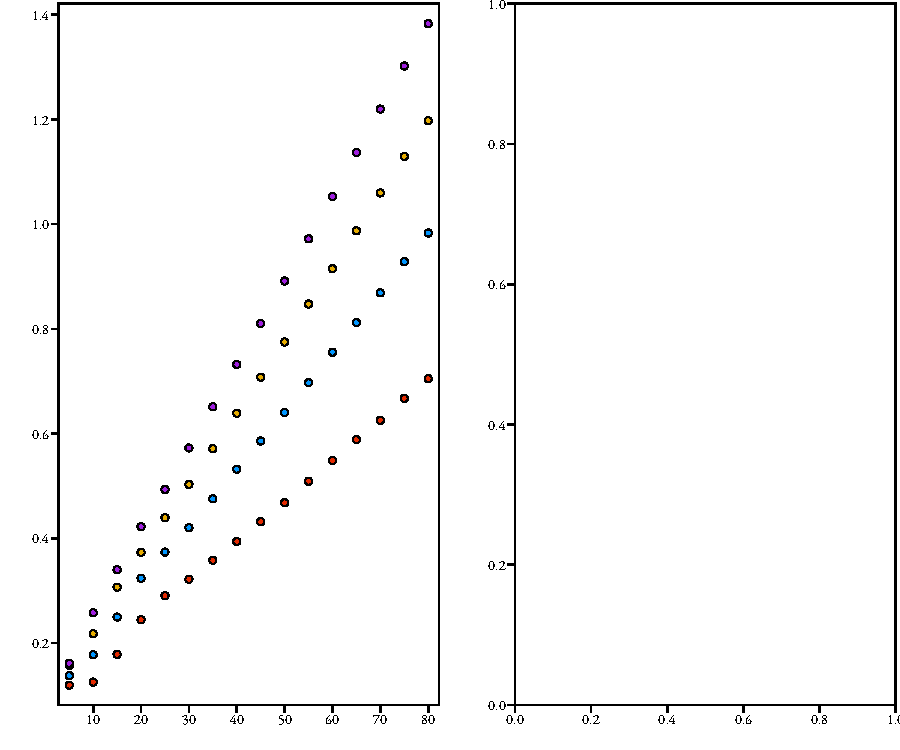
\includegraphics{nlp_profiling/nlp_profiling.pdf}
    \caption[
        The run time and peak memory consumption in computing the Hessian
        matrix for \acsp{FID} with differing numbers of datapoints and signals.
    ]
    {
        The run time and peak memory consumption in computing the Hessian
        matrix for \acsp{FID} with differing numbers of datapoints and signals.
        The \acp{FID} that were used to acquire these results are described in
        the main text.
        \textbf{a1.} and \textbf{b1.} The amount of time required to compute the
        Hessian for \ac{1D} and \ac{2D} \acp{FID}, respectively.
        \textbf{a2.} and \textbf{b2.} Equivalent plots showing the peak memory
        consumption in computing the Hessian.
    }
    \label{fig:nlp-profiling}
\end{figure}
A consideration of the burden on the \ac{CPU} and \ac{RAM} in computing the
Hessian matrix for \ac{1D} and \ac{2D} \acp{FID} (\cref{eq:hess}) is presented in
\cref{fig:nlp-profiling}.
It should be noted that for a typical \ac{NLP} routine, the Hessian will need
to be computed many times (on the order of magnitude of $10^2$ is common) so
while the times presented in the figure may seem small, a rather long total
time is possible for the \ac{NLP} routine if it takes seconds to compute the
Hessian once.
For the \ac{1D} case, simulated \acp{FID} were generated
with both a variable number of contributing signals: $M \in \lbrace 5k : k \in
\lbrace 1, 2, \cdots, 16 \rbrace \rbrace$ and datapoints: $N \in \lbrace 1024k
: k \in \lbrace 1, 2, \cdots, 8 \rbrace \rbrace$. For each \ac{FID}, the Hessian
was computed using a slight variant of the \texttt{obj\_grad\_hess\_1d}
function, given by Lines \ref{ln:objgradhessstart} to
\ref{ln:objgradhessend} in \cref{lst:obj-grad-hess}\footnote{
    The variant of this function neglected the computation of the objective and
    gradient, and returned only the Hessian.
}. There are 4 main steps in computing the Hessian matrix:
\begin{enumerate}
    \item Generation of all the first partial derivatives
        (\cref{eq:first-derivs}), which are stored in a $4M \times N$ array.
    \item Generation of all the non-trivially zero second partial
        derivatives (\cref{eq:second-derivs}), which are stored in a $10M
        \times N$ array.
    \item Computation of the non-zero elements of term \circled{2} in
        \cref{eq:hess}.
    \item Computation term \circled{1} in \cref{eq:hess}.
\end{enumerate}
These steps produce an exact Hessian. Neglecting steps 2 and 3 leads to the
formation of the approximated Hessian as described in
\cref{subsec:hess-approx}. \Cref{fig:nlp-profiling}.a1 shows that the
time to compute the Hessian matrix scales quadratically with $M$, and
linearly with $N$. The cause of this is the fact that the most time-consuming
aspect of the routine is step 4, which involves multiplying the $4M \times N$
matrix of first derivatives with its  $N \times 4M$ conjugate transpose, with a
complexity $\mathcal{O}(M^2N)$. The relative amount of the total run time which
is spent performing step 4 increases steadily as the model order increase, as
seen in \cref{tab:hess-steps}.
As such, for \ac{1D} \acp{FID}, it is
common, especially when the data comprises a large number of
signals, for the discrepancy in the amount of time to compute the true
Hessian relative to its approximation to be small. In these cases, it may be
valuable to compute the exact Hessian if it leads to a reduced number of
required iterations for convergence.
\begin{table}
    \begin{center}
        \begin{tabular}{ c c c c c c }
            \toprule
            $N$/$\Ntwo$ &
            $M$ &
            Step 1 &
            Step 2 &
            Step 3 &
            Step 4 \\
            \midrule
            \multicolumn{6}{c}{\textbf{1D Hessian}}\\
            \midrule
            2048 & 20 & 3.7\% & 9.6\% & 6\% & 76.4\% \\
            8192 & 20 & 3.5\% & 10.7\% & 6.3\% & 75\% \\
            2048 & 80 & 1\% & 3\% & 2\% & 92.6\% \\
            8192 & 80 & 1.2\% & 3.3\% & 1.9\% & 92.4\% \\
            \midrule
            \multicolumn{6}{c}{\textbf{2D Hessian}}\\
            \midrule
            64 & 20 & 8.2\% & 32.5\% & 18.5\% & 38.5\% \\
            256 & 20 & 12.3\% & 50.2\% & 21.3\% & 14.3\% \\
            64 & 80 & 10.8\% & 41\% & 24.3\% & 21.5\% \\
            256 & 80 & 14.9\% & 45.4\% & 24.1\% & 13.8\% \\
            \bottomrule
        \end{tabular}
    \end{center}
    \caption[
        A comparison of the relative times to perform the steps for
        computing the Hessian matrix for \acs{NLP}.
    ]{
        A comparison of the relative times to perform the steps for
        computing the Hessian matrix for \acs{NLP}, for selected pairings of
        $M$ and $N$ (\ac{1D})/$\Ntwo$ (\ac{2D}).
    }
    \label{tab:hess-steps}
\end{table}

To assess the effect of the number of signals and datapoints on Hessian
computation for \ac{2D} \acp{FID}, a series of signals were generated with a
fixed number of datapoints in the first dimension: $\None = 64$. \acp{FID} were
then constructed with the same values of $M$ as the \ac{1D} case, and $\Ntwo
\in \lbrace 64k : k \in \lbrace 1, 2, \cdots, 8 \rbrace \rbrace$. In contrast to
the \ac{1D} case, it is seen that the run time in computing the Hessian now
scales approximately linearly, rather than quadratically. Much more of the run
time is taken up by the first three steps in comparison; computing the
$6M\None\Ntwo$ first derivatives, $21M\None\Ntwo$ second derivatives, and
forming term \circled{2} all scale linearly with $M$, $\None$, and $\Ntwo$. The
relative times spent performing steps 2 and 3 compared with 1 and 4 imply that for
the \ac{2D} case (and for signals more more than 2 dimensions), a large saving
in computational time is typically achieved when the Hessian approximation
is utilised over the exact form.

Both the time- and space-complexity of computing the Hessian is found to be
roughly linear with both $M$ and the number of datapoints in each dimension
for \ac{1D} and \ac{2D} \acp{FID} (see Figures \ref{fig:nlp-profiling}.a2 and
\ref{fig:nlp-profiling}.b2). Most of the \ac{RAM} usage comes from storing
arrays of the first and second partial derivatives. In general, the typical
space requirements for both \ac{1D} and \ac{2D} \acp{FID} should be tolerable
on modern computers, which tend to possess at least \qty{8}{\gibi\byte} of
\ac{RAM}.

\section{Frequency Filtration}
\label{sec:filtering}
The previous section provides motivation for finding ways to reduce the
number of points in the signal and also the number of oscillators that the
signal contains. This has led to work on a procedure for generated
frequency-filtered ``sub-FIDs'' from the original data. A detailed description
of the filtering procedure is presented in this section.

\subsection{The \acl{VE}}
In brief, the filtering procedure  consists taking the \ac{FT} of the \ac{FID},
applying a band-pass filter on the spectral data to discard parts of not being
considered, and returning the spectrum back to the time-domain by an \ac{IFT}.
For a filtered \ac{FID} to be faithfully described by the model of a
summation of damped complex sinusoids, it is necessary that the
spectral peaks of interest lie effectively entirely within the filter
region\footnote{
    Lorentzian lineshapes tend to, but don't reach zero, as the distance from
    the maximum tends to $\infty$\cite{Tang1994}. However, as long as a
    sufficiently wide filtering is employed, the regions of the Lorentzian
    which do not pass through the filter can be assumed to be negligible.
}.
For absorptive Lorentzians, due to their characteristically narrow
linewidths, this is straightforward. However, for broader dispersive
Lorentzians, this is far more challenging. For this reason, generating
a spectrum in which only the real component is retained is desired.
Assuming the data has been phase-corrected, this will produce a
spectrum comprising only absorptive Lorentzians. The \ac{VE} has been employed
here, which has found application in the field of compressed sensing
NMR\cite{Mayzel2014,Golowicz2020,Luo2020}. This is a signal with double the
size as the original \ac{FID}, with the key characteristic that its \ac{FT} has
a real component which is equivalent to its counterpart derived from an
unaltered \ac{FID} (except it has double the points), and an imaginary
component of $0$s.

\subsubsection{The \acs{1D} \acl{VE}}
Assuming that a \ac{1D} \ac{FID} has been phase-corrected, such that $\bdphi =
\symbf{0} \in \mathbb{R}^M$, it can be denoted as
\begin{subequations}
    \begin{gather}
        \by =
        \symbf{\gamma} \odot
            \left(
                \symbf{c}^{(1)} + \iu \symbf{s}^{(1)}
            \right) + \bw, \\
        \symbf{\gamma} = \sum_m \bdam \exp \left(
                - \bdetaone \left[ m \right]
                \symbf{\tau}^{(1)}
            \right), \\
            \symbf{c}^{(1)}\text{/}\symbf{s}^{(1)} = \sum_m \cos\text{/}\sin \left(
                2 \pi \bdfone \left[ m \right] \symbf{\tau}^{(1)}_{\vphantom{t}}
            \right), \\
        \symbf{\tau}^{(1)} =
            \begin{bmatrix}
                0 & \Dtone & \cdots & \left(\None_{\vphantom{t}} - 1\right) \Dtone
            \end{bmatrix}\T
    \end{gather}
\end{subequations}
The frequency-dependence has been decomposed into its real and imaginary
components. With this in mind, a conjugate pair of signals are defined:
\begin{equation}
    \symbf{\psi}_{\pm} =
        \symbf{\gamma} \odot \left(
            \symbf{c}^{(1)} \pm \iu \symbf{s}^{(1)}
            \right) + \bw \equiv
            \Re\left(\by\right) \pm \iu \Im\left(\by\right)
\end{equation}
Two vectors $\lbrace \symbf{t}_{1}, \symbf{t}_2 \rbrace \in \mathbb{C}^{2
\None}$ are constructed using the conjugate pair:
\begin{itemize}
    \item $\symbf{t}_1$ is given by $\symbf{\psi}_+$ padded with zeros from below:
        \begin{equation}
            \symbf{t}_1 = \begin{bmatrix}
                \symbf{\psi}_+ \\ \symbf{0} \in \mathbb{C}^{\None}
            \end{bmatrix},\\
        \end{equation}
    \item $\symbf{t}_2$ is given by $\symbf{\psi}_{-}$ with its elements in
        reversed order ($\cdot^{{\leftrightsquigarrow}^{(1)}}$), padded with zeros
        from above, and finally subjected to a right circular shift by one
        element ($\cdot^{{\circlearrowright}^{(1)}}$):
        \begin{equation}
            \symbf{t}_2 = \begin{bmatrix}
                \symbf{0} \in \mathbb{C}^{\None} \\ \symbf{\psi}_-^{{\leftrightsquigarrow}^{(1)}}
        \end{bmatrix}^{{\circlearrowright}^{(1)}},
       \end{equation}
\end{itemize}
The \ac{VE} $\by_{\text{ve}}$ is then given by $\symbf{t}_1 +
\symbf{t}_2$, with the first element divided by $2$, which is equivalent to
\begin{equation}
    \by_{\text{ve}} =
    \begin{bmatrix}
        \Re\left( \by[0^{\vphantom{(1)}}] \right) &
        \by[1^{\vphantom{(1)}}] &
        \cdots &
        \by\left[\None - 1\right] &
        0 &
        \by\left[\None - 1\right]^* &
        \cdots &
        \by\left[1^{\vphantom{(1)}}\right]^*
    \end{bmatrix}\T.
\end{equation}
A signal of this form is illustrated in panel a of Figure \ref{fig:filtering}. As
eluded to already, the \ac{FT} of $\by_{\text{ve}}$ produces a spectrum
$\symbf{s}_{\text{ve}}$ such that $\Im\left(\symbf{s}_{\text{ve}}\right) =
\symbf{0}$, with $\Re\left(\symbf{s}_{\text{ve}}\right)$ featuring absorption
Lorentzian peaks (panel b of Figure \ref{fig:filtering}).


\subsubsection{The \acs{2D} \acl{VE}}
The \ac{VE} concept can be generalised to any number of dimensions, assuming
that a pair of amplitude-modulated signals exist for each indirect-dimension,
thus requiring a set of $2^{D-1}$ signals for a $D$-dimensional dataset.
\note{Maybe describe the general case in the appendix if you're bold enough?}
For the
\ac{2D} case, this corresponds to the pair of signals $\lbrace \bY_{\cos},
\bY_{\sin} \rbrace$, given by \eqref{eq:general-fid} with $D=2$ and $\zeta = \lbrace
\cos(\cdot), \sin(\cdot) \rbrace$, taking the forms (with noise neglected)
\begin{subequations}
    \begin{gather}
        \bY_{\cos} =
            \symbf{\Gamma} \odot
            \symbf{C}^{(1)} \odot \left(
                \symbf{C}^{(2)} +
                \iu \symbf{S}^{(2)}
            \right), \\
        \bY_{\sin} =
            \symbf{\Gamma} \odot
            \symbf{S}^{(1)} \odot \left(
                \symbf{C}^{(2)} +
                \iu \symbf{S}^{(2)}
            \right), \\
        \symbf{\Gamma} =
            \sum_m \bdam \left(
                \exp \left( -\bdetaonem \symbf{\tau}^{(1)} \right) \otimes
                \exp \left( -\bdetatwom \symbf{\tau}^{(2)} \right)
            \right), \\
        \symbf{C}^{(1)} \text{/} \symbf{S}^{(1)}
        = \sum_{m} \cos \text{/} \sin \left(2 \pi \bdfonem \symbf{\tau}^{(1)} \right)
            \otimes \symbf{1} \in \mathbb{C}^{\Ntwo}, \\
        \symbf{C}^{(2)} \text{/} \symbf{S}^{(2)} =
            \symbf{1} \in \mathbb{C}^{\None} \otimes
            \sum_{m} \cos \text{/} \sin \left(2 \pi \bdftwom \symbf{\tau}^{(2)} \right).
    \end{gather}
\end{subequations}
Four matrices are then constructed of the form
\begin{equation}
    \begin{gathered}
        \symbf{\Psi}_{\pm\pm} =
            \symbf{\Gamma} \odot \left(
                \symbf{C}^{(1)} \pm^{(1)} \hspace*{2pt} \iu \symbf{S}^{(1)}
                \right) \odot \left(
                    \symbf{C}^{(2)} \pm^{(2)} \hspace*{2pt} \iu \symbf{S}^{(2)}
                \right) \\
         \equiv
             \Re\left( \symbf{Y}_{\cos} \right)
             \pm^{(1)} \pm^{(2)} -
             \Im\left( \symbf{Y}_{\sin} \right)
             + \iu \left(
             \pm^{(1)}
             \Re\left( \symbf{Y}_{\sin} \right)
             \pm^{(2)}
             \Im\left( \symbf{Y}_{\cos} \right)
             \right),
    \end{gathered}
\end{equation}
from which the matrices $\symbf{T}_{1 \rightarrow 4} \in \mathbb{C}^{2 \None
\times 2 \Ntwo}$ are generated:
\begin{subequations}
    \begin{gather}
        \symbf{T}_1 =
        \begin{bmatrix}
            \symbf{\Psi}_{++} & \symbf{0} \\
            \symbf{0} & \symbf{0}
        \end{bmatrix}, \\
        \symbf{T}_2 =
        \begin{bmatrix}
            \symbf{0} & \symbf{0} \\
            \symbf{\Psi}_{-+}^{\leftrightsquigarrow (1)} & \symbf{0}
        \end{bmatrix}^{\circlearrowright (1)}, \\
        \symbf{T}_3 =
        \begin{bmatrix}
            \symbf{0} & \symbf{\Psi}_{+-}^{\leftrightsquigarrow (2)} \\
            \symbf{0} & \symbf{0}
        \end{bmatrix}^{\circlearrowright (2)}, \\
        \symbf{T}_4 =
        \begin{bmatrix}
            \symbf{0} & \symbf{0} \\
            \symbf{0} & \symbf{\Psi}_{--}^{\leftrightsquigarrow (1,2)}
        \end{bmatrix}^{\circlearrowright (1,2)}.
    \end{gather}
\end{subequations}
\note{Appendix for explicit forms of the matrices $\symbf{T}_{1-4}$}
The virtual echo is then given by $\symbf{Y}_{\text{ve}} = \sum_{i=1}^4
\symbf{T}_i$, with the first row and column divided by two. For a full outline
of the 2D filtering procedure, see Algorithm \ref{alg:filter-2d}.

It is possible to construct a virtual echo using an appropriate set of
phase-modulated signals too, which for the \ac{2D} case would be $\lbrace
\symbf{Y}_{\text{pos}}, \symbf{Y}_{\text{neg}}\rbrace$, given by
\eqref{eq:general-fid} with $D=2$ and  $\zeta = \lbrace \exp(\iu \cdot),
\exp(-\iu\cdot)\rbrace$. These can be used to generate an amplitude modulated pair via
\begin{subequations}
    \begin{gather}
        \symbf{Y}_{\text{cos}} = \frac{\symbf{Y}_{\text{pos}} + \symbf{Y}_{\text{neg}}}{2},\\
        \symbf{Y}_{\text{sin}} = \frac{\symbf{Y}_{\text{pos}} - \symbf{Y}_{\text{neg}}}{2\iu}.
    \end{gather}
\end{subequations}
\note{Should give $\zeta$ a dimension index, i.e.  $\zeta^{(1)}$}

\subsection{The filtering process}
Having constructed a virtual echo $\symbf{Y}_{\text{ve}} \in \mathbb{C}^{2\None
\times \cdots \times 2\ND}$, a spectrum with absorption Lorentzians is produced
with $\symbf{S}_{\text{ve}} = \FT\left(\symbf{Y}_{\text{ve}}\right)$. To filter
the spectrum, it is subjected to element-wise multiplication with a
super-Gaussian function. The super-Gaussian is defined by a centre
$c^{(d)} \in \mathbb{R}: 0 < c^{(d)} < 2 \Nd$ and a bandwidth  $b^{(d)} \in
\mathbb{N}: b^{(d)} < 2\Nd$ in each dimension (panel c of Figure
\ref{fig:filtering}):
\begin{subequations}
    \begin{gather}
        \symbf{G} = \bigotimes_{d=1}^D
            \symbf{g}^{(d)}, \\
        \symbf{g}_{\vphantom{t}}^{(d)}\left[ \nd \right] = \exp \left(
            -2^{p+1} \left(
                \frac{\nd - c^{(d)}_{\vphantom{t}}}{b^{(d)}}
            \right)^p
        \right)\ \forall \nd \in \lbrace 0, \cdots, 2 \Nd - 1 \rbrace.
        \label{eq:super-Gaussian-onedim}
    \end{gather}
\end{subequations}
An example of a \ac{1D} super-Gaussian is given in panel $c$ of Figure
\ref{fig:filtering}. The scalar $p \in \mathbb{R}_{>0}$ dictates the steepness
of the filter at the boundaries, with the function becoming more ``box-like''
as it increases. It is set to $40$ in this work and as the default in
\ac{EsPy}. Application of the super-Gaussian filter to $\symbf{S}_{\text{ve}}$
would lead to large sections of the filtered spectrum being $0$. This has an
undesired impact on the \ac{MDL}, as noise that has passed through filter (i.e.
the noise inside the region of interest) will now seem to resemble true signal,
as its amplitude is infinitely greater than the zeroed regions. A massive
over-estimation of model order therefore result. In order to obtain better
results from the model order selection, an array of synthetic \ac{AWGN} is
added to the filtered spectrum. To achieve this, a region in
$\symbf{S}_{\text{ve}}$ is specified which contains no discernible signal peaks
(referred to as the \emph{noise region}). The variance of this region
$\sigma^2$ is determined, and used to construct an array of values sampled from
a normal distribution with mean $0$ and variance $\sigma^2$,
$\symbf{W}_{\sigma^2} \in \mathbb{R}^{2 \None \times \cdots \times 2 \ND}$.
The filtered spectrum is then given by
\begin{equation}
    \widetilde{\symbf{S}}_{\text{ve}} = \symbf{S}_{\text{ve}} \odot \symbf{G} + \symbf{W}_{\sigma^2} \odot \left(\symbf{1} - \symbf{G} \right).
    \label{eq:Sve-tilde}
\end{equation}
Note that the noise array's magnitude at each point is attenuated by the value
of the super-Gaussian filter. Inside the region of interest ($\symbf{G}\left[
\none, \cdots, \nD \right] = 1$ ), the noise is nullified. See panel d of
Figure \ref{fig:filtering} for an example.

After filtering, $\widetilde{\symbf{S}}_{\text{ve}}$ is returned to the
time-domain by \ac{IFT}. The \ac{IFT} of a real-valued spectrum generates a
conjugate-symmetric signal. This is sliced in half in each dimension,
generating the final filtered sub-FID $\widetilde{\bY} \in
\mathbb{C}^{\None \times \cdots \times \ND}$:
\begin{equation}
    \widetilde{\bY} =
        \frac{1}{2^{D-1}}
        \IFT\left(\widetilde{\symbf{S}}_{\text{ve}}\right)
        \left[0:\None, \cdots, 0:\ND\right].
        \label{eq:yve-tilde}
\end{equation}
The scaling factor in \eqref{eq:yve-tilde} is to account for how many signals
have been combined to generate the \ac{VE}.

\begin{figure}
     \centering
     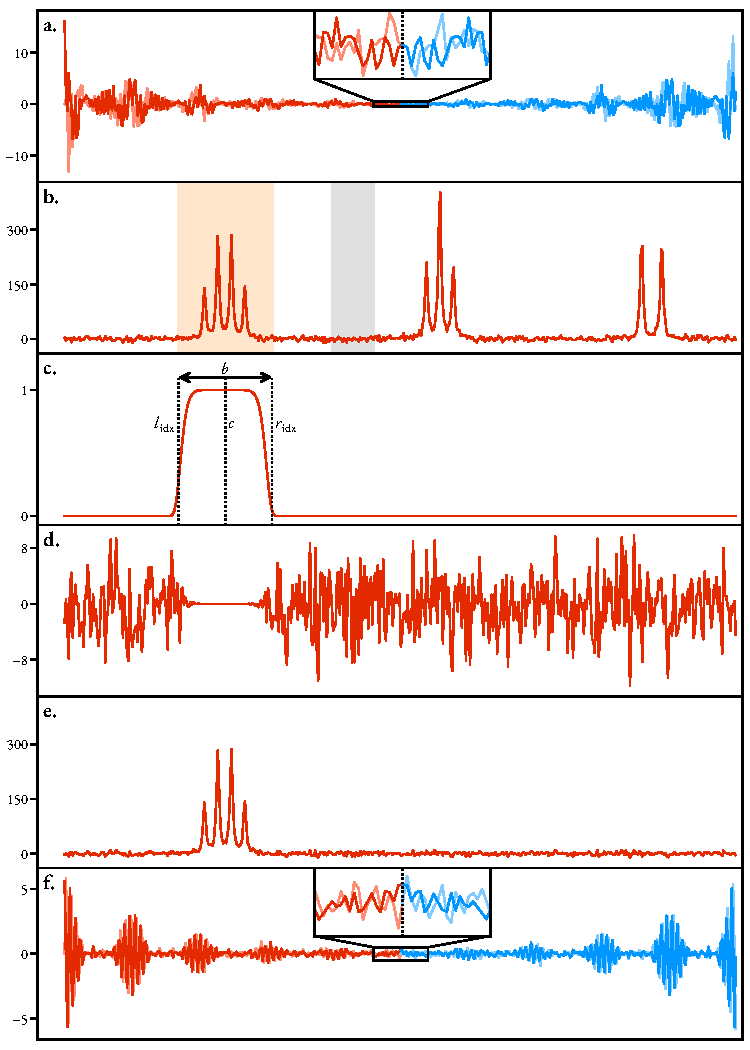
\includegraphics{filtering/filtering.pdf}
     \caption[
         An illustration of the filtering procedure applied to a \acs{1D}
         \acs{FID}.
     ]{
         An illustration of the filtering procedure applied to a \ac{1D}
         \ac{FID}.
         \textbf{a.} A \ac{VE} $\by_{\text{ve}}$, with the first and last
         $\None$ points coloured red and blue, respectively. The middle of the
         \ac{VE} is magnified to highlight its conjugate symmetry.
         \textbf{b.} The \ac{FT} of the \ac{VE}, $\symbf{s}_{\text{ve}}$.
         The region of interest (orange) and noise region (grey) are denoted.
         \textbf{c.} A super-Gaussian function used as a band-pass filter,
         $\symbf{g}$.
         \textbf{d.} \acs{AWGN} vector to be added to the filtered spectrum.
         The magnitude of the signal at each point is dependent on the
         corresponding super-Gaussian value.
         \textbf{e.} The filtered spectrum $\widetilde{\symbf{s}}_{\text{ve}}$,
         formed by applying the super-Gaussian filter, and adding the noise
         vector.
         \textbf{f.} The \ac{IFT} of the filtered spectrum,
         $\widetilde{\symbf{y}}_{\text{ve}}$, from which the final filtered
         signal $\widetilde{\symbf{y}}$ is obtained by extracting
         the first $\None$ points.
     }
     \label{fig:filtering}
\end{figure}

\subsubsection{Determining $c^{(d)}$ and  $b^{(d)}$}
The central index and bandwidth of the super-Gaussian filter function are given by the following expressions:
\begin{subequations}
    \begin{gather}
        c_{\vphantom{\text{idx}}}^{(d)} = \tfrac{1}{2} \left(l^{(d)}_{\text{idx}} + r^{(d)}_{\text{idx}}\right), \\
        b_{\vphantom{\text{idx}}}^{(d)} = l^{(d)}_{\text{idx}} - r^{(d)}_{\text{idx}},
    \end{gather}
\end{subequations}
where $l^{(d)}_{\text{idx}}$ and $r^{(d)}_{\text{idx}}$ denote the desired
indices where the filter's left and right bounds are located, respectively.
Array indices can be obtained from the corresponding spectral frequency
$f^{(d)}_{\unit{\hertz}}$ via
\begin{equation}
    \begin{gathered}
        f_{\text{idx}}^{(d)} =
            \left \lfloor
                \frac
                {
                    \left(2 \Nd_{\vphantom{d}} - 1\right)
                    \left(\fswd + 2 \left(\foffd - f_{\unit{\hertz}}^{(d)}\right) \right)
                }
                {2 \fswd}
            \right \rceil \\
        \forall f^{(d)}_{\unit{\hertz}} \in
            \left[\foffd - \tfrac{1}{2} \fswd, \foffd + \tfrac{1}{2} \fswd\right].
        \label{eq:fidx}
    \end{gathered}
\end{equation}
Conversion from \unit{\partspermillion} to array indices can be achieved by
replacing  $f_{\unit{\hertz}}$ in \eqref{eq:fidx} with
$f_{\unit{\partspermillion}} f_{\text{sfo}}$, where $f_{\text{sfo}}$ is the
transmitter frequency (\unit{\mega \hertz}).

\subsubsection{Spectrum slicing}
Thus far, the method described is able to reduce the model order of a given
signal, however the signal still comprises the same number of points. However
it is clear that there are a large number of points outside the region of
interest in $\widetilde{\symbf{S}}_{\text{ve}}$ that do not possess any
meaningful information. Discarding such points should then lead to filtered
\ac{FID} with the same information about the resonances of interest, but with
far fewer points. A slicing ratio is defined, $\xi \in \mathbb{R}: \xi > 1$,
which dictates the left and right indices at which the spectrum should be sliced
in each dimension:
\begin{subequations}
    \begin{gather}
        l_{\text{slice}}^{(d)} =
        \begin{cases}
            c_{\text{idx}}^{(d)} - \left \lfloor \frac{b^{(d)} \xi}{2} \right \rfloor &
            \text{if } \geq 0 \\
            0 & \text{otherwise}
        \end{cases} \\
        r_{\text{slice}}^{(d)} =
        \begin{cases}
            c_{\text{idx}}^{(d)} + \left \lceil \frac{b^{(d)} \xi}{2} \right \rceil &
            \text{if } \leq 2 \Nd - 1 \\
            2 \Nd - 1 & \text{otherwise}
        \end{cases}
    \end{gather}
\end{subequations}
The filtered spectrum is then sliced accordingly:
\begin{equation}
    \widetilde{\symbf{S}}_{\text{ve, slice}} =
        \widetilde{\symbf{S}}_{\text{ve}} \left[
            l_{\text{slice}}^{(1)} :
            r_{\text{slice}}^{(1)} + 1,
            \cdots,
            l_{\text{slice}}^{(D)} :
            r_{\text{slice}}^{(D)} + 1
        \right].
\end{equation}
The equivalent process is applied to $\widetilde{\symbf{S}}_{\text{ve,slice}}$
to generate the final filtered sub-\ac{FID}: \ac{IFT} followed by slicing in
half in each dimension.  It is also necessary to scale the signal by the ratio
of the number of points in the sliced spectrum and it's unsliced counterpart.
\begin{subequations}
    \begin{gather}
        \widetilde{\bY} =
            \prod_{d=1}^D \left(\frac{r_{\text{slice}}^{(d)} - l_{\text{slice}}^{(d)}}{2 \Nd}\right)
            \IFT \left( \widetilde{\symbf{S}}_{\text{ve, slice}} \right)
            \left[
                0 : \None_{\text{slice}}, \cdots, 0 : \ND_{\text{slice}}
            \right] \\
            \Nd_{\text{slice}} = \left \lfloor \frac{r_{\text{slice}}^{(d)} - l_{\text{slice}}^{(d)}}{2} \right \rfloor
    \end{gather}
\end{subequations}
Finally, the effective sweep widths and transmitter offsets will have been
altered by this process. The corrected values can be computed using
\begin{subequations}
    \begin{gather}
        f_{\text{sw,slice}}^{(d)} = \frac{r_{\text{slice}}^{(d)} - l_{\text{slice}}^{(d)}}{2 \Nd - 1} \fswd \\
        f_{\text{off,slice}}^{(d)} = \foffd + \frac{\fswd}{2} \left( 1 - \frac{l_{\text{slice}}^{(d)} + r_{\text{slice}}^{(d)}}{2 \Nd - 1}\right)
    \end{gather}
\end{subequations}

\section{Summary}
The \ac{MPM} is well established as an effective method for the parametric
estimation of signals in a number of disciplines.
One notable downside of the technique that has been realised while assessing
its effectiveness in parametrising \ac{NMR} \acp{FID} is its propensity to
return oscillators with unexpected phase behaviour, especially in scenarios
involving signals with similar frequencies, exhibiting considerable overlap in
the Fourier domain.
For this reason, using the result of the \ac{MPM} as an initial guess to feed
into a phase-variance regularised \ac{NLP} routine is proposed as a means of
returning improved parameter estimates. The theory underpinning the procedure
has been explored in this chapter.

The computational burden of running the procedure is large and often
insurmountable for complete \ac{NMR} datasets, which commonly comprise thousands of
points, and at least hundreds of contributing signals. Both the run time
and peak memory consumption of the \ac{1D} and \ac{2D} methods increase for \acp{FID} with more datapoints and more signals.
For this reason, a method to break the estimation problem into a
series of smaller, computationally tractable problems, through the construction
of frequency-filtered sub-\acp{FID}, has been introduced.

Having established an estimation routine, the next chapter focusses on its
performance in analysing \ac{1D} \ac{NMR} datasets, along with two specific
applications that arise.

% Algorithm \ref{alg:1d-2d-summary} provides an overview of the principal steps
% involved in the \ac{1D} estimation procedure. Detailed algorithms for each step
% are presented elsewhere in this text.

% \begin{algorithm}
%     \begin{algorithmic}[1]
%         \caption[
%             An overview of the estimation procedure outlined in this work.
%         ]{
%             An overview of the estimation procedure outlined in this work, for
%             the consideration of \ac{1D} \acp{FID}.
%         }
%         \label{alg:1d-2d-summary}
%         \Procedure{Estimate$1$D}{$
%             \by \in \mathbb{C}^{\None},
%             \symbf{R}_{\text{interest}} \in \mathbb{R}^{K \times 2},
%             \symbf{r}_{\text{noise}} \in \mathbb{R}^{2},
%             M \in \mathbb{N}_0
%             $
%         }
%             \State $l_{\text{idx,noise}}, r_{\text{idx,noise}} \gets r_{\text{noise}, 1}, r_{\text{noise}, 2}$;
%             \For{$k = 1, \cdots, K$}
%                 \State $l_{\text{idx}}, r_{\text{idx}} \gets r_{\text{interest}, k, 1}, r_{\text{interest}, k, 2}$;
%                 \State $\widetilde{\by} \gets \textsc{Filter}1\textsc{D}\left(
%                     \by,
%                     \right)
%                 $;
%                 \Comment{Algorithm \ref{alg:filter-1d}}
%                 \If{$M=0$}
%                     \State $M \gets \textsc{MDL}\left(\widetilde{\symbf{y}}\right)$;
%                     \Comment{\note{TODO}}
%                 \EndIf
%                 \State $\bthzero \gets \textsc{MPM}\left(\widetilde{\by}, M\right)$;
%                 \Comment{Algorithm \ref{alg:mpm}}
%                 \State $\bthstar, \symbf{\epsilon}^{(*)} \gets \textsc{NLP}\left(\widetilde{\by}, \bthzero\right)$;
%                 \Comment{Algorithm \ref{alg:nlp}}
%                 \State \textbf{return} $\bthstar, \symbf{\epsilon}^{(*)}$;
%             \EndFor
%         \EndProcedure
% %         \Statex
% %         \Procedure{Estimate$2$D}{$
% %             \bY_{\cos} \in \mathbb{C}^{\None \times \Ntwo},
% %             \bY_{\sin} \in \mathbb{C}^{\None \times \Ntwo},
% %             \symbf{R}_{\text{interest}} \in \mathbb{R}^{2 \times 2},
% %             \symbf{R}_{\text{noise}} \in \mathbb{R}^{2 \times 2},
% %             M \in \mathbb{N}_0
% %             $
% %         }
% %             \State $\widetilde{\bY} \gets \textsc{Filter}2\textsc{D}\left(
% %                 \bY_{\cos},
% %                 \bY_{\sin},
% %                 \symbf{R}_{\text{interest}},
% %                 \symbf{R}_{\text{noise}}
% %                 \right)
% %             $;
% %             \Comment{Algorithm \ref{alg:filter-2d}}
% %             \If{$M=0$}
% %                 \State $M \gets \textsc{MDL}\left(\widetilde{\bY}[:, 0]\right)$;
% %                 \Comment{Run the MDL on the first direct-dimension slice.}
% %             \EndIf
% %             \State $\bthzero \gets \textsc{MMEMPM}\left(\widetilde{\bY}, M\right)$;
% %             \Comment{Algorithm \ref{alg:mmempm}}
% %             \State $\bthstar, \symbf{\epsilon}^{(*)} \gets \textsc{NLP}\left(\widetilde{\bY}, \bthzero\right)$;
% %             \Comment{Algorithm \ref{alg:nlp}}
% %             \State \textbf{return} $\bthstar, \symbf{\epsilon}^{(*)}$;
% %         \EndProcedure
%     \end{algorithmic}
% \end{algorithm}



\chapter{Results and Applications Involving 1D Estimation}
\label{chap:results}

This chapter showcases results generated using the \ac{1D} estimation
technique outlined in the previous chapter. Furthermore, two means by
which the \ac{1D} estimation procedure can be harnessed as part of
specific applications are presented.
\Cref{sec:evaluation} provides some examples of how the estimation
routine performs on \ac{1D} \ac{NMR} datasets acquired using a standard
pulse-acquire experiment. \Cref{sec:seq} illustrates how the basic \ac{1D}
estimation routine
can be extended to enable the consideration of datasets comprising a series of
\acp{FID} which feature attenuations in signal amplitudes across increments,
including inversion recovery and diffusion experiments. Finally,
\cref{sec:bbqchili} describes a protocol to generate ultra-broadband spectra
through application of a single \ang{90} \acl{FS} pulse, which are devoid of
quadratic phase dependencies as well as baseline distortions.

All the results presented were produced on the same computer (see
\cref{rem:workstation}), using the \ac{EsPy} package which is
described in \cref{chap:nmrespy}. Details about the datasets generated are
provided in \cref{chap:datasets}.

\section{Conventional \ac{1D} Datasets}
\label{sec:evaluation}

As mentioned in \cref{subsec:phase-variance}, one of the disadvantages of
\ac{SVD}-based methods like the \ac{MPM} is their propensity to generate
parameter estimates featuring oscillators with spurious phase behaviour. Such
behaviour is most prevalent in \acp{FID} which (a) feature signals with very
similar frequencies and (b) that have a low \ac{SNR}.
To assess the effectiveness of including the phase variance-regularised
\ac{NLP} routine, comparisons are now made with results generated with the
\ac{MPM} in isolation.

For the experimental datasets considered (\cref{subsec:andro,subsec:cyclo}),
the data was pre-processed using \textsc{Bruker}'s \textsc{TopSpin} software,
using the series of commands \texttt{ft; pk; abs}; these perform \ac{FT},
automatic phase correction, and baseline correction, respectively. The data was
then converted back to the time-domain using \ac{IFT} prior to filtering and
estimation.

\subsection{``Twenty Signals''}
%%% Previously had this as landscape:
% \begin{sidewaysfigure}
%     \centering
%     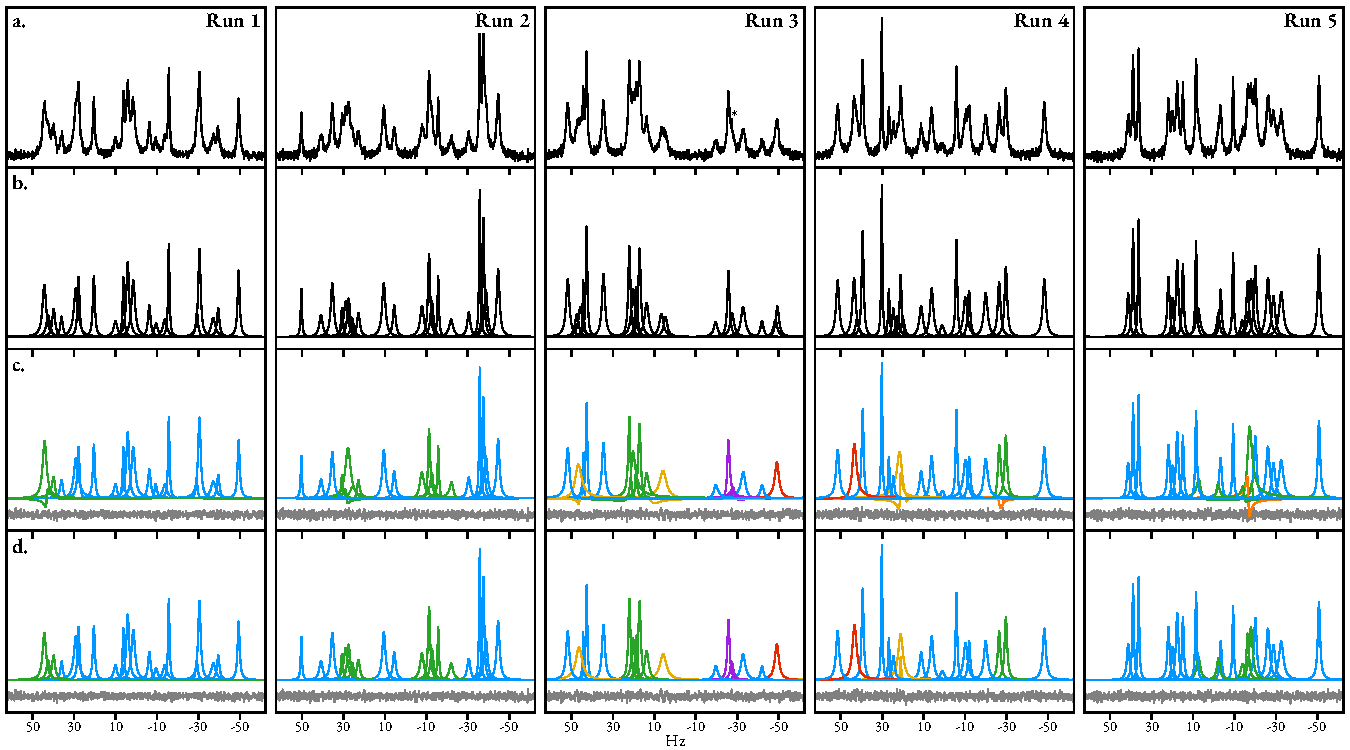
\includegraphics{mpm_vs_nlp/mpm_vs_nlp_landscape.pdf}
%     \caption[
%         The result of estimating a series of 5 simulated \acsp{FID}
%         using both the \acs{MPM} in isolation, and also with phase
%         variance-regularised \acs{NLP} used afterwards.
%     ]{
%         The result of estimating a series of 5 simulated \acp{FID} comprising
%         20 signals. See the main text for details on how the \acp{FID} were
%         constructed.
%         \textbf{a.} Spectra of the \acp{FID} generated.
%         \textbf{b.} Spectral lines corresponding to the set of signals
%         used to generate each \ac{FID}.
%         \textbf{c.} Plots of peaks for each oscillator generated using
%         the \acs{MPM}.
%         \textbf{d.} An equivalent plot for the result after applying phase
%         variance-regularised \acs{NLP}, using the \acs{MPM} result as an
%         initial guess.  Also included in c and d are the
%         residual between the data and the estimated model (grey
%         line). The colouring of the oscillators in c and d is described
%         in the main text.
%     }
%     \label{fig:mpm_vs_nlp}
% \end{sidewaysfigure}
\begin{figure}
    \centering
    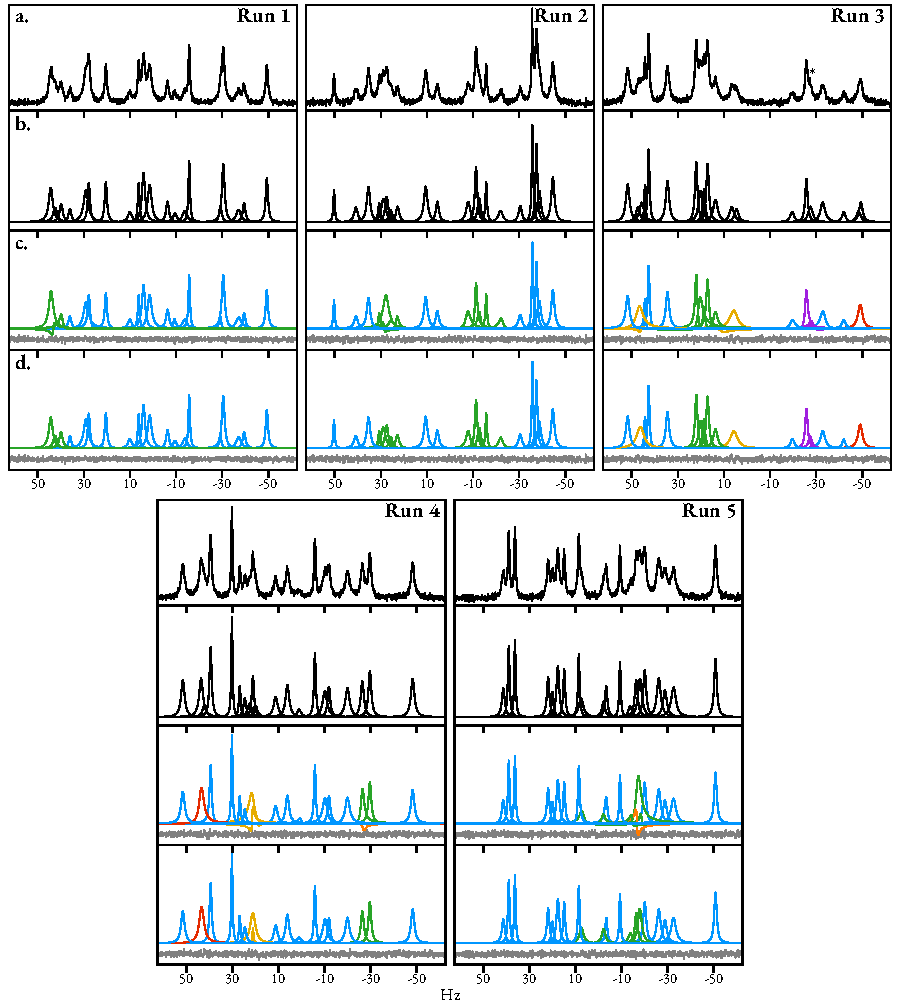
\includegraphics{mpm_vs_nlp/mpm_vs_nlp_portrait.pdf}
    \caption[
        The result of estimating a series of 5 simulated \acsp{FID}
        using both the \acs{MPM} in isolation, and also with phase
        variance-regularised \acs{NLP} used afterwards.
    ]{
        The result of estimating a series of 5 simulated \acp{FID} comprising
        20 signals. See the main text for details on how the \acp{FID} were
        constructed.
        \textbf{a.} Spectra of the \acp{FID} generated.
        \textbf{b.} Spectral lines corresponding to the set of signals
        used to generate each \ac{FID}.
        \textbf{c.} Plots of peaks for each oscillator generated using
        the \acs{MPM}.
        \textbf{d.} An equivalent plot for the result after applying phase
        variance-regularised \acs{NLP}, using the \acs{MPM} result as an
        initial guess.  Also included in c and d are the
        residual between the data and the estimated model (grey
        line).
        \correction{
            Blue oscillators are those produced by the MPM which closely agree
            with a true signal.  Green oscillators are affected notably by the
            NLP routine, and end up in good agreement with a true signal.
            Orange oscillators were excessive oscillators generated by the MPM,
            which were removed during the NLP routine, leading to a
            parsimonious fit of the remaining (green) oscillators in the
            frequency neighbourhood.  Yellow oscillators denote cases where the
            number of oscillators produced by the MPM matched the number of
            true signals in a given frequency neighbourhood. However one of the
            oscillators was removed during the NLP routine, leading to an
            under-fit of the neighbourhood.  Red oscillators denote an
            under-fit of a frequency neighbourhood by the MPM.  Purple
            oscillators denote an over-fit of a frequency neighbourhood by the
            MPM, with none of the oscillators being removed during NLP
            (\textit{cf.} orange oscillators which are removed during NLP).
        }
    }
    \label{fig:mpm_vs_nlp}
\end{figure}
A series of five simulated \acp{FID} were constructed using
\cref{eq:hypercomplex-fid} with $D=1$. For each \ac{FID}, a model order
of $M=20$ was used, the number of points sampled was $N = 1024$, the sweep
width was $\fsw=\qty{125}{\hertz}$, and the transmitter offset was $\foff
= \qty{0}{\hertz}$.  Each oscillator was assigned a phase of \ang{0}, while the
amplitudes, frequencies and damping factors were drawn at random from the
following distributions
$\forall m \in \lbrace 1, \cdots, 20\rbrace$:
$a_m \sim \mathcal{U}(1, 5)$, $f_m \sim \mathcal{U}(\qty{-55}{\hertz},
\qty{55}{\hertz})$, $\eta_m \sim \mathcal{U}(\qty{2}{\per\second},
\qty{8}{\per\second})$. The frequencies were subjected to an additional
constraint; no two signals were permitted to have frequencies that
differed by less than $\nicefrac{4 \fsw}{N} \approx \qty{0.49}{\hertz}$.
Each noiseless \ac{FID} $\bx$ was then corrupted with \ac{AWGN}, with a target
\ac{SNR} of \qty{25}{\deci\bel}, such that the desired noise variance for each
\ac{FID} was given by (\emph{cf.} \cref{eq:snr,eq:snr-db}):
\begin{equation}
    \sigma^2 = \frac{1}{20^{2.5} \times 1024}
        \sum_{n=0}^{1023} \lvert x_n \rvert^2.
\end{equation}
The spectra of the simulated \acp{FID} are presented in
\cref{fig:mpm_vs_nlp}.a, with the set of oscillator peaks which contribute
to the spectrum in \cref{fig:mpm_vs_nlp}.b. With the criteria used to
constructed the datasets, it can be seen they feature signals which often
suffer from severe overlap, with the high noise variance compounding the
opportunity to clearly identify all contributing signals.

For each \ac{FID}, the \ac{MPM} was performed, assuming a model order of
30, constituting a considerable over-fit of oscillators. The \ac{MDL} tended to
produce under-estimates of $M$ when applied to these \acp{FID}, so the
hard-coded value was used instead to ensure sufficient oscillators were given
to the model. The under-estimates were likely due to the
high \ac{SNR} of the signals\,---\,recall the red signal in \cref{fig:mdl}\,---\,in
conjunction with severe signal overlap. When an excessive model order is
provided to the \ac{MPM}, it is typical that oscillators corresponding to the
noise subspace of the data matrix $\Hy$ are characterised by small amplitudes
and/or very small damping factors. For this reason, prior to subjecting the
\ac{MPM} result to \ac{NLP}, oscillators which satisfied $a_m < 0.1$ and/or
$\eta_m < \qty{0.7}{\per\second}$ were removed from the parameter set. The
individual oscillators which make up the \ac{MPM} result after purging spurious
components are displayed in \cref{fig:mpm_vs_nlp}.c, along with the
residual between the data and the estimated model (i.e. the sum of all
oscillator peaks).

The \ac{MPM} consistently generated models which agreed well with the data
in a least squares sense, as as evidenced by the residuals in
\cref{fig:mpm_vs_nlp}.c.
However, it can be seen that in several spectral regions across the datasets,
especially ones that are highly crowded, oscillators possess parameters which
deviate significantly from the true signal parameters used to constructed the
\acp{FID}.
Most notably, individual oscillator phases regularly stray far from \ang{0},
and their associated amplitudes are often considerably different too.
In \cref{fig:mpm_vs_nlp}.c, blue oscillators are those which
are in very close agreement with a particular true signal in the data.
Oscillators with other colours are not in agreement with a true signal,
with the different colourings described shortly.
The desired outcome of the \ac{NLP} routine is for it to adjust the
parameters associated with non-blue oscillators in \cref{fig:mpm_vs_nlp}.c such
that they agree with true signals, while having little to no effect on those of
the blue oscillators. The results after application of \ac{NLP} are provided in
\cref{fig:mpm_vs_nlp}.d.

In discussing the outcome of the routine, it will be helpful to employ the
concept of a \emph{frequency neighbourhood}, a loose term which describes a
small, continuous subset of frequencies within the spectral window. As the
\ac{NLP} routine involves taking small steps
in parameter space over a number of iterations, it is unlikely that an
oscillator which starts off with a frequency far away from a particular
frequency neighbourhood will eventually enter it. As such, in order for the
\ac{NLP} routine to successfully estimate the signals within a given frequency
neighbourhood of the data, sufficient model oscillators need to present within
the neighbourhood in the initial guess.

Cases where the
\ac{MPM} generated enough oscillators for a given frequency neighbourhood,
albeit with parameters which noticeably deviate from the true signals are
coloured either green or yellow. Green oscillators are those which the \ac{NLP} routine
was able to adjust so as to to achieve agreement with true signals;
they indicate improvements to the estimation result in comparison with the \ac{MPM}
in isolation. Conversely, yellow oscillators denote cases where, though
sufficient oscillators existed in the frequency neighbourhood in the initial
guess, the \ac{NLP} routine evolved such that at least one of the oscillators
was driven by the phase variance constraint to acquire a negative amplitude,
leading to it being removed from the parameter set. This typically occurred with
oscillators that had an initial phase which was either $>
\nicefrac{\pi}{2}$\,\unit{\radian}, or $< -\nicefrac{\pi}{2}$\,\unit{\radian}.
Therefore, yellow oscillators indicate cases where the final result
under-fit the dataset.

There are a couple of instances, denoted by red oscillators,
where the \ac{MPM} assigned too few oscillators to a particular frequency
neighbourhood, and as such the \ac{NLP} routine would not have been able to
yield any major improvement. This occurred in what can safely be described as
fiendishly difficult cases, where severe signal overlap and low \ac{SNR} make
it very difficult to associate certain spectral regions with more than one
signal by eye.

The final two oscillator groupings, coloured purple and orange respectively,
indicate scenarios where the \ac{MPM} generated more oscillators than true
signals in a given frequency neighbourhood (i.e. the data was over-fit in these
regions). Orange
oscillators we purged by the \ac{NLP} routine as they acquired negative
amplitudes. This enabled parsimonious fits of the relevant frequency neighbourhoods by
the oscillators which remained, i.e. the green oscillators in close proximity
to the orange ones in \cref{fig:mpm_vs_nlp}.c. Finally, the purple oscillators
denote the one
occasion (Run 3) where an over-fit occurred, and the model order was not
successfully reduced by the \ac{NLP} routine. One of the purple oscillators in
the \ac{MPM} appears to agree closely with a significant ``blip'' in the noise,
denoted by an asterisk in \cref{fig:mpm_vs_nlp}.a.
The over-fit has therefore occurred because this noise component was
incorporated into the final result; it was neither purged based on the
amplitude and damping factor criteria outlined above, nor by acquiring a
negative amplitude during \ac{NLP}.

\subsection{Andrographolide}
\label{subsec:andro}
\begin{figure}
    \centering
    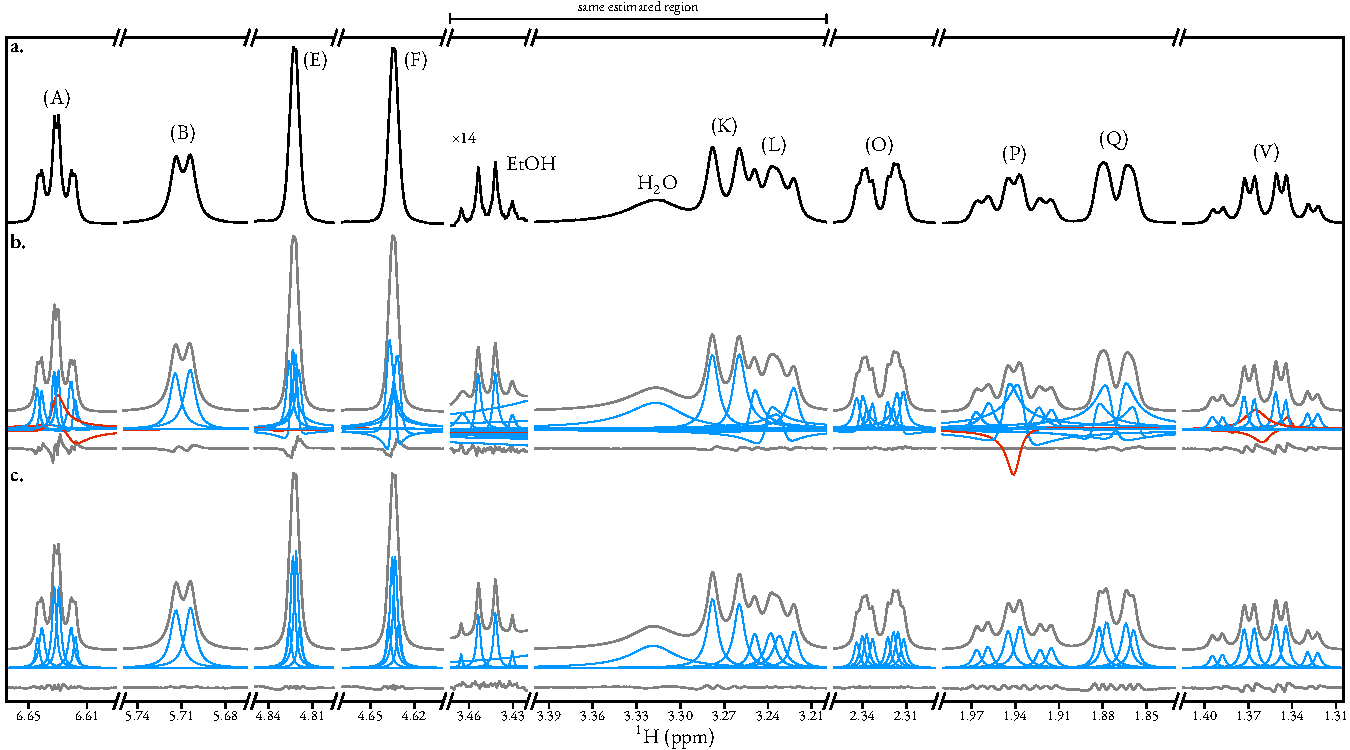
\includegraphics{andrographolide_onedim/andrographolide_onedim.pdf}
    \caption[
        The result of applying the estimation routine to selected regions of a
        pulse-acquire dataset of andrographolide.
    ]{
        The result of applying the estimation routine to selected regions of a
        pulse-acquire dataset of andrographolide in \acs{DMSOd6}.
        \textbf{a.} The structure of andrographolide.
        \textbf{b.} Spectral regions considered.
        \textbf{c.} The result of applying the \acs{MPM} to the regions, with
        the model order predicted using the \acs{MDL}. Blue and red lines denote
        individual oscillator peaks, while the grey line above is the sum of all
        oscillators. They grey line below is the residual between the data and
        the model.
        \textbf{d.} The result after convergence of the \acs{NLP} routine, again
        with the model above and residual below.
        Red peaks in b correspond to oscillators which acquire negative
        amplitudes and are removed during the \acs{NLP} routine.
        One of the estimated regions has been split in two in the
        figure to save space, with one half, featuring a signal from ethanol,
        being magnified.
    }
    \label{fig:andro-onedim}
\end{figure}
\Cref{fig:andro-onedim} illustrates the outcome of applying the
estimation routine to a \textsuperscript{1}H dataset of
andrographolide (\cref{fig:structures}.a) in \acs{DMSOd6}, acquired with
a \qty{600}{\mega\hertz} spectrometer.
Various spectral regions were chosen for study, and for each one, a
frequency-filtered sub-\ac{FID} was produced using the approach in
\cref{sec:filtering}.
The \ac{MPM} was used to generate an initial guess of parameters, using the
\ac{MDL} to predict the model order in each case. The result of applying the
\ac{MPM} are presented in \cref{fig:andro-onedim}.b. The initial guess
was then subjected to \ac{NLP}, giving rise to the result
\cref{fig:andro-onedim}.c.

The \ac{NLP} routine was effective at resolving the spurious phase behaviour
often generated by the \ac{MPM}.
The estimation method's ability to parametrise signals with high
dynamic range and high variation of damping factors is also evidenced;
a broad intense singlet from water, and a low-intensity quartet from
residual ethanol in the sample, present in the same sub-\ac{FID}, could both
estimated admirably for example.
For some of the sub-\acp{FID} considered, the \ac{MPM} output featured
oscillators, commonly with very high damping factor and/or phases far from
\ang{0}, which were removed during the \ac{NLP} routine (see the red
peaks in panel b). The removal of these, along with the enforcement
of consistent oscillator phases, leads to parameter
estimates which describe the apparent multiplet structures associated with each
spin well. \Cref{tab:andro-multiplets} provides an overview of the
most significant couplings associated with the spins giving rise to the
multiplet structures considered.
\begin{table}
\centering
\begin{tabular}{c c c}
\hline
Spin  & Coupling partners & Multiplet structure \\
\hline
\multicolumn{3}{c}{\textbf{Andrographolide}}\\
\hline
(A) & (D)\textsuperscript{long}, (M)\textsuperscript{vic}, (N)\textsuperscript{vic} & ddd (\emph{dt}) \\
(B) & (D)\textsuperscript{ex} & d \\
(E) & (F)\textsuperscript{vinyl} \dots & d\dots \\
(F) & (E)\textsuperscript{vinyl} \dots & d\dots \\
(K) & (J)\textsuperscript{gem}, (H)\textsuperscript{ex} & d \\
(L) & (C)\textsuperscript{ex}, (T)\textsuperscript{180}, (U)\textsuperscript{60} & dd \\
(O) & (P)\textsuperscript{gem}, (R)\textsuperscript{60}, (V)\textsuperscript{60} & ddd \\
(P) & (O)\textsuperscript{gem}, (R)\textsuperscript{60}, (V)\textsuperscript{180} & ddd (\emph{dt}) \\
(Q) & (M)\textsuperscript{vic}, (N)\textsuperscript{vic} \dots & dd\dots \\
(V) & (O)\textsuperscript{60}, (P)\textsuperscript{180}, (R)\textsuperscript{g}, (W)\textsuperscript{180} & dddd (\emph{dq}) \\
\hline
\multicolumn{3}{c}{\textbf{Cyclosporin A}}\\
\hline
(A) & diastereotopic pair on \textsuperscript{\textbeta}C & dd \\
(B) & ---''--- & dd \\
(C) & ---''--- \& amide proton & ddd (\emph{dt}) \\
(D) & proton on \textsuperscript{\textbeta}C \& amide proton & dd \\
(E) & methyl protons on \textsuperscript{\textbeta}C \& amide proton & dq \\
(F) & ---''--- & dq (\emph{quintet}) \\
\hline
\end{tabular}
\caption[
    The major coupling partners associated with spins in andrographolide and
    cyclosporin A, along with the multiplet structures that arise.
]{
    The major coupling partners associated with spins in andrographolide and
    cyclosporin, considered in \cref{fig:andro-onedim,fig:cyclosporin}
    respectively, along with the multiplet structures that arise.
    For andrographolide, coupling partners are labelled as follows:
    \textsuperscript{vinyl} geminal coupling between two vinylic protons,
    \textsuperscript{ex} geminal coupling between two protons, with one
    bonded to an oxygen, leading to exchange decoupling\cite[Section
    2.6.1.5]{Claridge2016},
    \textsuperscript{gem} geminal coupling between two spins whose dihedral
    angle is not fixed,
    \textsuperscript{long} long-range coupling,
    \textsuperscript{vic} vicinal coupling,
    \textsuperscript{60} geminal coupling, with a fixed dihedral angle of
    \ang{60} between the spins,
    \textsuperscript{180} geminal coupling, with a fixed dihedral angle of
    \ang{180} between the spins.
    All cyclosporin couplings for the spins considered are geminal couplings.
    In cases where the observed multiplet structure is different to the true
    structure, the observed structure is is in brackets. Ellipses denote cases
    where more (long-range) coupling partners are likely, based on the
    estimation result generated/the appearance of the spectrum, though these
    have not been explicitly assigned.
}
\label{tab:andro-multiplets}
\end{table}

One of the most challenging aspects of estimating \ac{NMR} signals is
the common presence of signals within the dataset that have incredibly similar
frequencies due to the influence of scalar couplings.
Molecules with fused ring systems such as andrographolide are prime examples of spin
systems which generate such datasets, as they tend to have very dense coupling
networks leading to complex multiplet structures. Furthermore, fused systems often
exhibit appreciable long-range couplings (between spins separated by four or
more bonds) alongside ubiquitous two-bond (\emph{geminal}) and three-bond
(\emph{vicinal}) couplings. Long range couplings can be particularly challenging to
resolve, as they are often of a comparable magnitude to the spectral resolution
($\nicefrac{\fsw}{N}$), making individual signals barely perceptible.

Take the multiplet structure from spin (Q) as an example of a particularly
challenging estimation problem.
(Q) has separate vicinal couplings to the
diastereotopic protons (M) and (N); these are the couplings to
(Q) of greatest magnitude. If these were the only couplings, a doublet of doublets
(dd) structure would be expected, which is what has been generated by
the estimation routine.
However, a comparison of the data and
the model indicates that there is a clear discrepancy between the two,
evidenced by systematic deviations in the residual; this feature hints at an
under-fit of the data.
% The \ac{MPM} generated oscillators with phases deviating far from \ang{0},
% which enabled good agreement with the data in a residual sense, though of
% course such a set of oscillators is unrealistic in the context of a phased
% \ac{FID}.
Long-range couplings with magnitudes that are large enough to influence the
appearance of (Q)'s multiplet structure are likely to be present, which leads
to frequency neighbourhood in which all contributing signals are too poorly
resolved to realistically gleam any further meaningful information, at least at
the field strength used.

As a second illustration, the multiplet structure corresponding to spin (V) is also
under-fit, this time because the presence of a number of couplings of similar
magnitude leads to resonances coalescing at roughly the same frequency. A
multiplet structure featuring 16 resonances forming in ``dddd'' structure is
expected. However, 3 of the couplings are of similar magnitudes, such that
many of the contributing signals coalesce to form what is apparently a quartet
of doublets (dq).
The estimation routine was able to resolve this dq structure,
however the large deviations in the residual again imply that under-fitting has
occurred, and each oscillator in the parameter set is in fact being used to fit
two or more signals present in the \ac{FID}. Again, at the field strength used
to acquire the \ac{FID}, it is unlikely that an accurate resolution of all 16
signals by estimation is feasible.

% At this point, with two examples provided of cases where poor \ac{RSS} fits
% have resulted, one may question whether the underlying model is actually suited
% to describe the data.
% There is for example precedent for fitting oscillators with non-exponential
% decay profiles\,---\,profiles which lead to Voigt and Gaussian spectral
% lineshapes are common\,---\,to improve the model fit\cite{Sima2007}.
% However, for some multiplet structures in Figure \ref{fig:andro-onedim},
% exceptionally good agreement between the model and data are made, using a
% parsimonious set of parameters.
With three couplings of different magnitude, spin (O) exhibits a ``ddd''
multiplet structure in which all 8 signals are discernible. The \ac{NLP}
routine performed well in taking the initial guess from the
\ac{MPM}\,---\,featuring the correct number of oscillators albeit with
spurious phases\,---\, and generating a well-phased set of oscillators defining
the ddd structure, with a very small associated residual. This highlights that
in cases where all signals present in a given frequency neighbourhood are
resolvable, effective estimation results are achievable.

\subsection{Cyclosporin A}
\label{subsec:cyclo}
\begin{figure}
    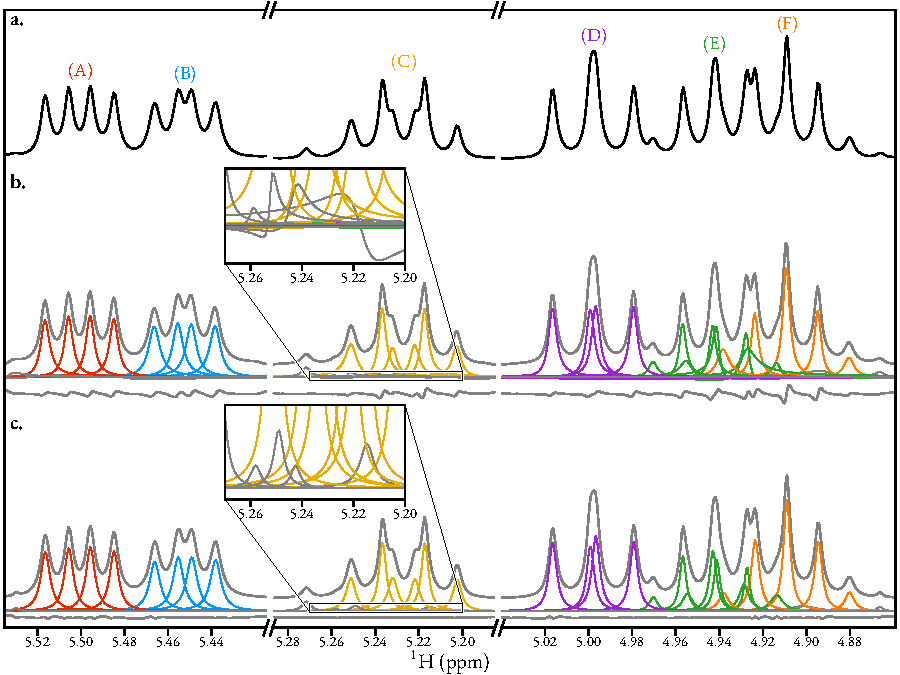
\includegraphics{cyclosporin/cyclosporin.pdf}
    \caption[
        The result of applying the estimation routine to selected regions of a
        pulse-acquire dataset of cyclosporin A.
    ]{
        The result of applying the estimation routine to selected regions of a
        pulse-acquire dataset of cyclosporin A in benzene-d\textsubscript{6}.
        \textbf{a.} The structure of cyclosporin A, with relevant proton
        environments highlighted.
        \textbf{b.} Spectral regions considered.
        \textbf{c.} The result of applying the \acs{MPM} on the regions, with
        the model order predicted using the \acs{MDL}.
        The grey lines above and below the individual oscillator peaks denote
        the sum of all oscillators and the residual between the data and the
        model, respectively.
        \textbf{d.} The result after convergence of the \acs{NLP} routine,
        presented in the same format as panel c.
        Coloured oscillators have been mapped to particular cyclosporin A
        environments. Grey oscillators are not associated with
        cyclosporin A; these are likely due to impurities in the sample.
    }
    \label{fig:cyclosporin}
\end{figure}
The estimation routine was also applied to selected regions of a
\proton\ pulse-acquire dataset of cyclosporin A
(\cref{fig:structures}.b), a cyclic peptide comprising 11 amino
acids, in benzene-d\textsubscript{6}.
The regions considered all comprise
signals arising from protons bound to C\textsuperscript{\textalpha} atoms in
the peptide backbone\cite{Verma2018}.
The estimation procedure used was equivalent to
that used for the andrographolide example.

For the most downfield region
considered, featuring signals from spins (A) and (B), the \ac{MPM} performed
admirably, with the two well-resolved dd multiplet structures present
accurately parametrised by the 8 oscillators in the model; the \ac{NLP} routine
hardly perturbed the initial guess as a result.

In the middle region, which features a doublet of triplets (dt) multiplet structure
from spin (C), low intensity ``shoulders'' are noticeable;
these are likely from low-concentration impurities in the sample. The \ac{MPM}
was able to resolve the dt structure, and characterise
some low intensity signals too, though the phases of these are highly
inconsistent, with a knock-on effect for the relative amplitudes of signals
describing the dt structure (these are expected to abide by the ratio
1:2:1:1:2:1). The \ac{NLP} routine, by enforcing low phase variance in the
oscillators, subtly adjusted the parameter estimate to achieve a set of
oscillator amplitudes that are more consistent with this ratio.

The most downfield region contains three separate multiplet structures
featuring significant signal overlap in the Fourier domain, particularly
involving those corresponding to spins (E) and (F).
The \ac{MPM} produced sufficient oscillators to model these
structures (see \cref{tab:andro-multiplets} for an outline of the structures
present).
However, particularly in the most crowded section around
\SIrange{4.96}{4.92}{\partspermillion} it can be seen that certain oscillators
have phases which noticeably deviate from \ang{0}. In applying the \ac{NLP}
routine, not only did the phases become more consistent,
but the oscillator amplitudes also become more agreeable.
For example, the highest- and lowest-frequency model oscillators
associated with the 1:3:6:3:1 quintet of spin (F) (denoted by
\textdagger\ in Figures \ref{fig:cyclosporin}.b and \ref{fig:cyclosporin}.c)
acquire amplitudes which are much closer in value after \ac{NLP}, as expected.
The most
notable flaw in the final result is associated with the two oscillators marked
by \textdaggerdbl\ in panel c, both of which are associated with the
1:3:1:3:3:1:3:1 dq structure from spin (E). A 1:3 amplitude ratio is expected
between these oscillators. However, in the final \ac{NLP} result, these
had an unexpected ratio of $\approx 1:1$. It is not surprising
that greater deviations from the expected result occur in more heavily crowded spectral
regions, since there is a larger set of values in the parameter space which
will lead to acceptable fits of the data in an \ac{RSS} sense. Nonetheless,
armed simply with knowledge that the data is phased, the routine performs
admirably in highlighting  how the spectrum breaks down into its various
signal components. An improved estimation result could be attained by
supplying the \ac{NLP} routine with more knowledge in the form of parameter
constraints. While this has not been implemented in this work, it is discussed
in \cref{sec:future-work} as a possible pursuit for the future.

\section{Amplitude-Attenuated Datasets}
\label{sec:seq}
There are a number of \ac{NMR} experiments in which the
variation of a particular pulse sequence parameter over a number of iterations
leads to the generation of a series of
\acp{FID} with the same form except for discrepancies in their amplitudes.
In this section, an extension of the established \ac{1D} estimation
technique is described, facilitating the analysis of datasets acquired using
these experiments.
After the most prominent examples of this class of experiment have been
introduced, the methodology of the technique to analyse them is described.
Finally, the technique's performance when applied to both simulated and
experimental datasets is showcased.

\subsection{Relaxation Experiments}
\label{subsec:relaxation_experiments}
Any spin system which has been perturbed from its equilibrium position will
eventually return to equilibrium due to relaxation. As introduced in
\cref{chap:intro}, the simplest model of relaxation centers around two
processes: longitudinal relaxation and transverse relaxation, whose rates are
quantified by the times $T_1$ and  $T_2$ respectively.
Numerous factors affect these times including the rate at which
\correction{the molecule that the spin is associated with}\label{corr:spin-molecule}
tumbles in space, and its electronic environment.
The $T_1$ and $T_2$ values of the spins in a sample provide valuable insight
into the chemical system being studied, and can also help to guide
spectroscopists in the determination of optimal pulse sequence
parameters\footnote{
    For example, after a pulse sequence has been run, it is necessary to include a
    delay (called the \emph{relaxation delay}) prior to
    re-running it, to enable the spin system's longitudinal magnetisation to
    sufficiently recover. Having an understanding of the $T_1$ values
    associated with a sample can help to determine a relaxation delay which is
    long enough to facilitate sufficient recovery, but that is not excessive, to
    avoid an experiment time which is longer than necessary.
}.

\subsubsection{Measuring $T_1$: Inversion Recovery}
\label{subsec:invrec}
The inversion recovery experiment involves the simple pulse sequence $\ang{180}
\rightarrow \tau \rightarrow \ang{90} \rightarrow \tone$, where $\tone$ is the
period during which \ac{FID} acquisition takes place. The initial
\ang{180} pulse inverts the magnetisation, so that it is along the $-z$ axis in
the context of the Bloch model. During $\tau$, the spin system undergoes
longitudinal
relaxation, with the spin state populations gradually being driven back to
their equilibrium configuration. The \ang{90} pulse rotates the magnetisation
into the transverse plane, enabling detection. The resultant phase and
magnitude of each signal is directly related to the amount of time that
longitudinal relaxation is allowed to occur. With $\tau = \qty{0}{\second}$,
signals with maximal amplitude, but phases of \ang{180} (equivalent to a
negative amplitude) will result\footnote{
    Here it is being assumed that a perfect $\ang{90}_y$ pulse is being
    applied, such that magnetisation along $-z$ will be rotated onto the $-x$
    axis.
}. At the other extreme of $\tau \gg T_1$,
the spin system will have reverted
back to equilibrium, such that the signals will also have maximal amplitudes,
but phases of \ang{0}. By sequentially adjusting $\tau$ in a
\ac{2D} experiment, a series of \acp{FID} will be obtained in which the intensity
of a given signal, arising from a spin with longitudinal relaxation time $T_1$,
will vary according to
\begin{equation}
    a\left(\tau\right) = a_{\infty} \left( 1 - 2 \exp\left( -\frac{\tau}{T_1}\right) \right),
\end{equation}
where $a_{\infty}$ is the intensity of the signal when the spin system
has returned to equilibrium. Note that $a(0) = -a_{\infty}$, as the magnetisation
has been completely inverted, and no time has been allowed for longitudinal
relaxation to take place. An example of a series of spectra acquired using a
(simulated) inversion recovery experiment is given by
\cref{fig:five-multiplets-invrec}.d.

\subsubsection{Measuring $T_2$: \acs{CPMG}}
\label{subsec:cpmg}
Inspired by the inversion recovery experiment, one might assume
that the pulse sequence $\ang{90} \rightarrow \tau \rightarrow \tone$ would be
effective for  $T_2$ determination.
\correction{
    However, this is not so; due to chemical shift evolution in the $\tau$
    period, large first-order phase effects will result, with the extent of the
    phase being dependent on $\tau$. Furthermore, the effects of
    J-modulation would cause additional phase-modulations within multiplet
    structures, which could not be resolved by phase correction.
}\label{corr:T2-issues}
Beyond phase issues with the resultant data, the
presence of field inhomogeneities will cause relaxation at a faster rate than
anticipated; the effect of field inhomogeneities is incorporated into the
``observed'' transverse relaxation time, $T_2^* < T_2^{\vphantom{*}}$\footnote{
    $T_2^*$ is defined by the expression
    $\nicefrac{1}{T_2^*} \coloneq \nicefrac{1}{T_2} + \gamma \Updelta B_0$,
    where $\Updelta B_0$ is the variation in magnetic field strength across the
    sample volume.
    \label{fn:t2-star}
}~\cite{Chavhan2009}. All the effects noted above can be nullified if rapid
refocussing is applied, by subjecting the spin system to a train of spin
echoes. The classic route to $T_2$ measurement is the \ac{CPMG}
experiment~\cite{Carr1954,Meiboom1958}, comprising $\ang{90}_x \rightarrow
\left[ \tau \rightarrow \ang{180}_y \rightarrow \tau \right]_n \rightarrow
\tone$, where the spin echo duration $\tau$ is short and fixed, and the number
of cycles $n$ can be varied to alter the total evolution time. The number of
\ac{CPMG} cycles applied affects the intensity of the resulting signal
according to
\begin{equation}
    a(n) = a_0 \exp\left(-\frac{2 \tau n}{T_2}\right),
\end{equation}
where $a_0$ is the intensity where no spin echo cycles were employed, such that
the pulse sequence is reduced to the standard pulse-acquire experiment. Recent
enhancements to the \ac{CPMG} approach, including the \ac{PROJECT} pulse
sequence~\cite{Aguilar2012} are also well-suited to $T_2$ determination.

\subsection{Diffusion Experiments}
\label{subsec:diffusion_experiments}
\ac{NMR} is well established as a means of determining the rates of
translational diffusion of chemical species~\cite{Johnson1999,Morris2009b}.
The rate of translation of a species is given by the translational
diffusion coefficient, $D$ (\unit{\meter\squared\per\second})~\cite[Chapter
19]{Atkins2014}.
The first illustration of the determination of the diffusion coefficient using
\ac{NMR} came from Stejskal and Tanner, in which they described the \ac{PGSE}
pulse sequence~\cite{Stejskal1965} (\cref{fig:diffusion_sequences}.a).
The \ac{PGSE} sequence consists of a conventional spin-echo ($\ang{90}_x
\xrightarrow{\tau} \ang{180}_y \xrightarrow{\tau} \text{acquire}$), with
\acp{PFG} applied after each of the \ac{RF} pulses.
As a simple overview of how the pulse sequence works, consider a single spin on
resonance with the transmitter (i.e. its rotating frame frequency is zero) in a
sample tube at position $z \in [-\nicefrac{l_z}{2}, \nicefrac{l_z}{2}]$ along
the main field axis, where $l_z$ is the length of the sample lying within the
receiver coil (typically about $\qty{1.5}{\centi\meter}$).
After the \ang{90} pulse, the magnetisation will be $-M_y$.
During the first \ac{PFG}, the spin's resonance frequency will become
$\omega_{\text{PFG}} = -\gamma g z$, where $g$ is the strength of the \ac{PFG}
(\unit{\tesla\per\meter})\footnote{
    Gradient strengths are often expressed in the non-\ac{SI} units of
    \unit{\gauss\per\centi\meter}, which is equivalent to
    \qty[print-unity-mantissa = false]{e-2}{\tesla\per\meter}.
}.
Assuming the gradient is applied for a time $\delta$, the spin will
precess by the angle $\alpha = -\gamma g z \delta$. After the \ang{180}
pulse, the spin's magnetisation will be as follows:
\[
    -M_y
    \xrightarrow{\text{PFG}} -M_y \cos(\alpha) + M_x \sin(\alpha)
    \xrightarrow{\ang{180}_y} -M_y \cos(\alpha) - M_x \sin(\alpha).
\]
Suppose the spin has moved to a new position $z + \Updelta_z$
between the end of the first gradient and the beginning of the second.
Application of the second gradient will cause precession by the angle
$\beta = -\gamma g (z + \Updelta_z) \delta$:
\begin{equation*}
   \begin{split}
        \xrightarrow{\text{PFG}}
            &-M_y \cos(\alpha)\cos(\beta) +
            M_x \cos(\alpha)\sin(\beta) -
            M_x \sin(\alpha)\cos(\beta) -
            M_y \sin(\alpha)\sin(\beta)\\
        &= -M_y \cos(\gamma g \delta \Updelta_z) -
           M_x \sin(\gamma g \delta \Updelta_z),
   \end{split}
\end{equation*}
Therefore the \acp{PFG} have been been employed to encode the
change in $z$-position of the spin after a known amount of time.
Extending this idea to an ensemble of many identical non-interacting spins,
which will translate by different extents between the \acp{PFG}, individual
spin contributions to the bulk magnetisation will become dephased, leading to
an attenuation of the amplitude of the resulting \ac{FID}. For species which
diffuse at a faster rate, such that typical deviations $\Updelta_z$ are
larger, the dephasing effect is more severe, such that a more rapid attenuation
results for a given increase in $g$.

\begin{figure}
   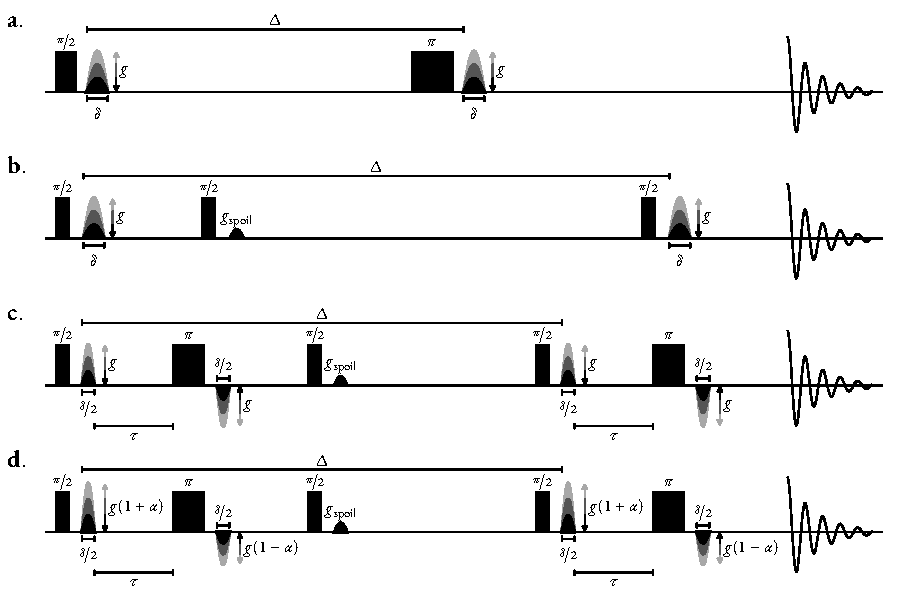
\includegraphics{diffusion_sequences/diffusion_sequences.pdf}
   \caption[
       Pulse sequences used for the determination of translational diffusion constants.
   ]{
       Pulse sequences used for the determination of translational diffusion constants.
       \textbf{a.} \acs{PGSE},
       \textbf{b.} \acs{PGSTE},
       \textbf{c.} \acs{PGSTEBP},
       \textbf{d.} One-shot DOSY.
       \ac{RF} pulses are denoted by solid rectangles. Diffusion-encoding
       gradients are denoted by sine-bell shapes with varying shades,
       indicating that the intensity ($g$) is incremented to create a \ac{2D}
       dataset. Spoiler gradients are denoted by solid black sine-bell shapes.
   }
   \label{fig:diffusion_sequences}
\end{figure}

Through consideration of the Bloch-Torrey equations, which
extend the classic Bloch equations to account for the effects of diffusion on
magnetisation~\cite{Torrey1956}, the following equation, known as the
\emph{Stejskal-Tanner equation}, may be derived:
\begin{equation}
    a(g) = a_0 \exp \left(- \gamma^2 \delta^2 g^2 D \left(\Updelta -
    \frac{\delta}{3}\right)\right),
    \label{eq:stejskal_tanner}
\end{equation}
where
$a_0$ is the amplitude of a given signal without the application of \acp{PFG},
$\delta$ is the duration of each \ac{PFG} (\unit{\second}), and
\correction{
    $\Updelta$ is the time from the start of the first \ac{PFG} to the start
    of the next,
}\label{corr:diffusion-time} often known as the \emph{diffusion time}
(\unit{\second}).
While \cref{eq:stejskal_tanner} is widely stated in the diffusion \ac{NMR}
literature, it is only strictly applicable when the \ac{PGSE} sequence is used,
and \acp{PFG} with rectangular amplitude profiles are applied\footnote{
    Rectangular \acp{PFG} (i.e. those in which there is an infinitesimal time
    to rise to full strength, and to fall back to zero) are technically
    impossible to achieve as they would require gradient coils with zero
    inductance, though in practice it is possible to generate gradients with
    behaviour close to this.
}. As will be discussed soon, the exact form of the pulse sequence impacts the
functional form by which $a(g)$ varies.

Tanner introduced a variant of the original \ac{PGSE} experiment called
\ac{PGSTE}~\cite{Tanner1970} (\cref{fig:diffusion_sequences}.b). Instead
of the diffusion period being bisected by a
\ang{180} pulse, \ac{PGSTE} features two \ang{90} pulses at the beginning and
end of the diffusion period.
Hence, the extent of signal loss due to relaxation is affected by $T_1$ in
\ac{PGSTE}, as opposed to $T_2$ in \ac{PGSE}. \ac{PGSTE} is therefore favoured
in scenarios where $T_1 \correction{\gg} T_2$\label{corr:t1-t2}, as improved data sensitivity is achievable.

Both \ac{PGSE} and \ac{PGSTE} employ \emph{monopolar} \acp{PFG} for diffusion
encoding.
Experiments also exist which employ
\emph{bipolar} gradient elements, which consist of a
\ac{PFG}, followed by a \ang{180} pulse, and then a second \ac{PFG} with the
opposite polarity to the first~\cite{Cotts1989,Wu1995}. The \ac{PGSTEBP} experiment
(\cref{fig:diffusion_sequences}.c) can be thought of as the bipolar analogue of
\ac{PGSTE}.
Bipolar gradients are useful in circumstances where it is important to purge
the effects of static gradients in the sample, caused by field inhomogeneities.
Morris and coworkers have developed the \emph{one-shot}
experiment~\cite{Pelta2002} (\cref{fig:diffusion_sequences}.d), which requires a
single transient per gradient strength (i.e. there is no requirement for a
phase-cycling scheme).  This is achieved through the use of bipolar gradients
which comprise asymmetrical \acp{PFG} with relative powers $1 + \alpha : 1 -
\alpha$ for some $\alpha \in (0, 1)$; commonly, $\alpha=0.2$.

The most common means of conducting a diffusion experiment is to run one of the
pulse sequences mentioned above (or variants thereof) with $g$ varied across
increments.
\correction{
    The \ac{FID}'s signal amplitudes always abide by the following general form
    of the Stejskal-Tanner equation, regardless of the exact pulse sequence
    used:
}\label{corr:stej-tann}
\begin{equation}
    a(g) = a_0 \exp\left(- c g^2 D\right),
\end{equation}
for some constant $c$ \correction{(\unit{\second\per\tesla\squared})}\label{corr:c-unit}.
The functional form of $c$ depends on the type of experiment used, as well as
the amplitude profile (\emph{shape}) of the \acp{PFG}.
A consideration of the Bloch-Torrey equations for a given experiment is
necessary, with an extensive overview provided by Sinnaeve for most diffusion
NMR experiments~\cite{Sinnaeve2012}. In general, $c$ is as follows:
\begin{equation}
    c = \gamma^2 \delta^2 \sigma^2 \Updelta^{\prime}.
    \label{eq:stejskal_tanner_generic}
\end{equation}
$\sigma$ is the \emph{shape factor} of the \acp{PFG} (\textit{vide infra}),
and $\Updelta^{\prime}$ is the effective time that diffusion is allowed
to occur. Examples of the form that $\Updelta^{\prime}$ takes include:
\begin{equation}
    \Updelta^{\prime} =
    \begin{cases}
        \Updelta + 2 \left(\kappa - \lambda\right) \delta &
        \text{\ac{PGSE}, \ac{PGSTE}}\\
        \Updelta + \frac{\left(2 \kappa - 2 \lambda - 1\right)\delta}{4} - \frac{\tau}{2} &
        \text{\ac{PGSTEBP}} \\
        \Updelta + \frac{\left(\kappa - \lambda\right)
            \left(\alpha^2 + 1\right) \delta}{2} +
        \frac{\left(\delta + 2 \tau\right)\left(\alpha^2 - 1\right)}{4} &
        \text{One-shot}
    \end{cases}.
    \label{eq:Delta-prime}
\end{equation}
$\tau$ is the delay between the initial \ac{PFG} and the \ang{180} pulse in
experiments with bipolar gradients.
The factors $\sigma$,  $\lambda$, and $\kappa$ are related to the shape
function $s(\epsilon) : \epsilon \in [0, 1]$ of the \ac{PFG}, which describes
the variation of the gradient amplitude as a function of its progression.
For a rectangular gradient, $s(\epsilon) = 1 \forall \epsilon$, whereas for a
sine-bell gradient, $s(\epsilon) = \sin(\pi \epsilon)$. The cumulative
distribution of the shape function is given by:
\begin{equation}
    S(\epsilon) = \int_0^{\epsilon} s\left(\epsilon^{\prime}\right)
            \mathrm{d} \epsilon^{\prime} \quad \forall \epsilon \in [0, 1].
\end{equation}
The corresponding definition of $S$ for a discrete gradient made of $N$
steps, $\symbf{s} \in \mathbb{R}^{N}$, is
\begin{equation}
    S_n =
        \frac{1}{n} \sum_{i = 1}^{n} s_i \quad
        \forall n \in \left\lbrace 1, \cdots, N\right\rbrace,
\end{equation}
$\sigma$, $\lambda$, and $\kappa$ are related to the shape function's
cumulative distribution as follows:
\begin{subequations}
    \begin{gather}
        \sigma = S(1),\\
        \lambda = \frac{1}{\sigma} \int_0^1 S(\epsilon) \mathrm{d} \epsilon,\\
        \kappa = \frac{1}{\sigma^2} \int_0^1 S^2(\epsilon) \mathrm{d} \epsilon,
    \end{gather}
\end{subequations}
with their discrete counterparts being:
\begin{subequations}
    \begin{gather}
        \sigma = S_{N} \\
        \lambda = \frac{1}{\sigma N} \sum_{n = 1}^{N} S_n
            = \frac{1}{\sigma N} \sum_{n=1}^{N}
            \left(\frac{1}{n} \sum_{i=1}^{n} s_i\right) \\
        \kappa = \frac{1}{\sigma^2 N} \sum_{n = 1}^{N} S^2_n
            = \frac{1}{\sigma^2 N} \sum_{n = 1}^{N}
            \left(\frac{1}{n} \sum_{i=1}^{n} s_i\right)^2.
    \end{gather}
\end{subequations}
For \acp{PFG} with a symmetrical shape, $\lambda = \nicefrac{1}{2}$. $\kappa$
is typically equal to or close to $\nicefrac{1}{3}$. It can now be seen that
the original Stejskal-Tanner equation for the
\ac{PGSE} experiment (\cref{eq:stejskal_tanner}) comes from
inserting \cref{eq:Delta-prime} into \cref{eq:stejskal_tanner_generic},
assuming a rectangular shape factor for the \acs{PFG}:
$\sigma = 1$,  $\lambda = \nicefrac{1}{2}$, and  $\kappa = \frac{1}{3}$.
In many situations,  $\Updelta$
dominates in the expression of $\Updelta^{\prime}$, and so ensuring the correct
form of $c$ could be seen as excessive. However, especially when  $\Updelta$ is
not orders of magnitude greater than $\delta$, the exact form of
$\Updelta^{\prime}$ used in \cref{eq:stejskal_tanner_generic} will be
important for accurate measurements of the diffusion coefficient.

\subsection{Analysing the Datasets}
Determining the quantity of interest from the above experiments is most
typically done using the following procedure:
\begin{enumerate}
    \item Each of the \acp{FID} in the series is processed using the same protocol,
        leading to a set of \ac{1D} spectra.
    \item Peak-picking is performed to locate the chemical shift values which
        correspond to signals of interest within the spectra.
    \item For each chemical shift corresponding to a peak location, the values
        of the spectra are extracted across increments. The relevant
        function describing how the amplitude is expected to decay across
        increments is then fit to these values, to extract the quantity of
        interest.
\end{enumerate}
This method is \emph{univariate} in the sense that it considers a single sample
(chemical shift) in isolation from the rest of the data.
It is popular to visualise the result of univariate fitting by plotting \ac{2D}
pseudo-spectra, featuring axes denoting (a) chemical shift, and (b)
the parameter of interest. Distributions taking
into account the predicted value of interest and the associated uncertainty
are plotted at each chemical shift.
In the context of diffusion \ac{NMR}, this form of data analysis is
referred to as \ac{DOSY}~\cite{Morris2009b}.
The \ac{DOSY} approach works well in cases where peaks of interest are intense
and well-resolved. However, when there is considerable peak overlap, accurately
determining the parameter of interest associated with a given signal becomes
more challenging, since nearby signals will influence the rate of amplitude
decay. An aggregated value of the decay rates of the contributing signals
will be predicted using the above approach.
In such cases, it is possible to instead fit
a superposition of functions to the spectral amplitudes, as a means of
separating out contributions from the overlapping signals~\cite{Nilsson2006}.
However, this process is usually only effective when the data has very high
\ac{SNR}, and the quantities of interest associated with the overlapping
signals differ considerably.

An alternative approach
is to use a \emph{multivariate} analysis, in which entire spectrum is
considered holistically, and an attempt is made to decompose the spectrum into
components with different decay rates. Prominent examples of multivariate methods
developed for diffusion data analysis are \ac{DECRA}~\cite{Windig1998} and
\emph{speedy} component resolution (\acs{SCORE})~\cite{Nilsson2008}, an
improvement of the original \acs{CORE}~\cite{Stilbs1996,Stilbs1996b}.
\acused{SCORE}\acused{CORE}
Multivariate techniques tend to only be effective in situations where a
few (2 or 3) different signal decay rates are present. In diffusion
\ac{NMR}, each molecule in the sample will give rise to the same decay rate
across its signals (effects such as chemical exchange can lead to exceptions to
this: \cref{fig:andrographolide-dosy} provides an example of this). As such,
only a few decay rates typically govern the form of diffusion data, making
multivariate approaches feasible.
Conversely, multivariate methods are generally unsuitable for inversion
recovery and \ac{CPMG} datasets: each spin in a sample will possess different
$T_1$ and $T_2$ values, such that a far greater number of decay rates will be
present.

\subsection{Methodology}
\label{subsec:seq-method}
A straightforward extension of \ac{1D} parametric estimation
provides a route to estimating amplitude-attenuated datasets in a
fashion with similarities to the traditional univariate (\ac{DOSY}) approach.
The theory of this method will now be discussed.

Suppose one of the experiments mentioned above is run with $K \in \mathbb{N}$
increments,
such that there is a vector  $\symbf{p} \in \mathbb{R}^K$ comprising the
values of the pulse sequence variable used to acquire each \ac{1D} \ac{FID} in
the data.  The complete dataset is expected to take the form $\symbf{Y} \in
\mathbb{C}^{K \times N}$ in which the value of the pulse sequence variable
affects the amplitudes of the contributing signals:
\begin{equation}
    \begin{gathered}
        y_{k,n} = \sum_{m=1}^{M} a_{k,m} \exp(\iu \phi_m)
        \exp((2 \pi \iu (f_m - \foff) - \eta_m) n \Dt),\\
        \forall k \in \lbrace 1, \cdots, K \rbrace,\ \forall n \in \lbrace 0,
        \cdots, N-1 \rbrace.
    \end{gathered}
\end{equation}
$\symbf{A} \in \mathbb{R}^{K \times M}$ is a matrix of the signal amplitudes
across the \acp{FID}:
\begin{equation}
    \symbf{A} =
    \begin{bmatrix}
        a_{1,1} & a_{1,2} & \cdots & a_{1,M}\\
        a_{2,1} & a_{2,2} & \cdots & a_{2,M}\\
        \vdots & \vdots & \ddots & \vdots\\
        a_{K,1} & a_{K,2} & \cdots & a_{K,M}
    \end{bmatrix}
\end{equation}
A complete parameter vector for the dataset is given by $\bth \in
\mathbb{R}^{(K + 3)M}$:
\begin{equation}
    \bth =
    \begin{bmatrix}
        \symbf{a}_1 & \cdots & \symbf{a}_K & \bdphi\T & \bdf\T & \bdeta\T
    \end{bmatrix}\T,
\end{equation}
where $\symbf{a}_k \in \mathbb{R}^M$ denotes the relevant row in $\symbf{A}$.
The amplitudes are a function of the pulse sequence variable with the following
form:
\begin{equation}
    a_{k,m} = a_{0,m} \mathcal{A} (\psi_m \hspace*{2pt} | \hspace*{2pt} p_k).
\end{equation}
$\symbf{a}_0 \in \mathbb{R}^{M}$ is a vector of the ``maximal
amplitudes'' of the signals, and $\symbf{\psi} \in \mathbb{R}^M$ is a vector
of the parameter of interest ($T_1$,  $T_2$, $D$) associated with
each signal. $a_{0,m}$ can be thought of as the largest
possible amplitude that could be obtained for signal $m$ with the given
pulse sequence:
\begin{itemize}
    \item In an inversion recovery experiment, the largest amplitude is
        achieved as $\tau \rightarrow \infty$, as the spin system will have
        returned back to equilibrium prior to the \ang{90} pulse.
    \item With \ac{CPMG} experiments, the largest amplitude will occur when
        $n = 0$, as no time is designated for transverse
        relaxation to take place.
    \item For diffusion experiments, the largest amplitude is achieved when
        $g=0$, since no diffusion-induced dephasing of spins will have
        occurred.
\end{itemize}
The function $\mathcal{A}$ describes how the amplitudes of signals are
attenuated by the experimental variable, and has a form which is intimately
linked to the type of experiment. For the experiments described in
\cref{subsec:relaxation_experiments,subsec:diffusion_experiments},
the forms of $\mathcal{A}$ are listed in \cref{tab:seq-equations}.
\begin{table}
    \begin{center}
        \begin{tabular}{ccccccc}
            \hline
            Experiment &
            $p$ &
            $\psi$ &
            $\mathcal{A}(\psi | p)$ &
            $\frac{\partial \mathcal{A}(\psi | p)}{\partial \psi}$ &
            $\frac{\partial^2 \mathcal{A}(\psi | p)}{\partial \psi^2}$ \\ \hline
            Inv. Recov.&
            $\tau$ &
            $T_1$ &
            $\left(1 - 2 \exp \left(-\frac{\tau}{T_{1}}\right)\right)$ &
            $-\frac{2 \tau}{T_1^2} \exp\left(-\frac{\tau}{T_1}\right)$ &
            $\frac{2 \tau}{T_1^3} \exp\left(-\frac{\tau}{T_1}\right)\left(2 - \frac{\tau}{T_1}\right)$\\
            \acs{CPMG} &
            $n$ &
            $T_2$ &
            $\exp\left(-\frac{2 \tau n}{T_2}\right)$ &
            $\frac{2 \tau n}{T_2^2}\exp\left(-\frac{2 \tau n}{T_2}\right)$ &
            $\frac{2 \tau n}{T_2^3}\exp\left(-\frac{2 \tau n}{T_2}\right)
            \left( \frac{2 \tau n}{T_2} - 2 \right)$ \\
            Diffusion &
            $g$ &
            $D$ &
            $\exp\left(-c g^2 D\right)$ &
            $-c g^2 \exp\left(-c g^2 D\right)$ &
            $c^2 g^4 \exp\left(-c g^2 D\right)$ \\
            \hline
       \end{tabular}
       \caption[
           The various functional forms of $\mathcal{A}$ according to the
           different amplitude-attenuating NMR experiments considered.
       ]
       {
           The various functional forms of $\mathcal{A}$ according to the
           different amplitude-attenuating NMR experiments considered, along
           with the first and second derivatives, which are required to extract
           estimates of $\psi$ using \ac{NLP}.
       }
       \label{tab:seq-equations}
    \end{center}
\end{table}

\subsubsection{Estimating the Datasets}
The close relationship between the \acp{FID} within the dataset means that
completely estimating all of them separately, without exploiting information
from previously estimated \acp{FID}, is unnecessary.
Instead, after the first increment is estimated without prior knowledge,
yielding $\bth_{1} \in \mathbb{R}^{4M}$, the phases, frequencies and damping
factors, all of which are anticipated to remain the same across the
\acp{FID}, are fixed.
Subsequent parameter estimates are determined by taking the result from
the previous \ac{FID}, and subjecting it to \iac{NLP} routine in which only
the amplitudes are optimised. Thus, estimating each subsequent iteration
is reduced to the problem\footnote{
    $\mathcal{F}$ in \cref{eq:fidelity-amp} reads as ``the fidelity
    with respect to the amplitudes $\bda$, given phases $\bdphi_{1}$,
    frequencies $\bdf_{1}$, damping factors  $\bdeta_{1}$, and \ac{FID}
    $\by_k$''. The fidelity has exactly the same mathematical form as
    \cref{eq:fidelity}, though it has been emphasised that the phases,
    frequencies and damping factors are no longer variables to be optimised,
    but fixed parameters.
}
\begin{equation}
    \symbf{a}_k = \argmin_{\bda \in \mathbb{R}^M}
        \mathcal{F}(\bda \hspace*{2pt} | \hspace*{2pt}
        \bdphi_{1}, \bdf_{1}, \bdeta_{1}, \by_k)\quad\forall k \in \lbrace2, \cdots, K\rbrace.
        \label{eq:fidelity-amp}
\end{equation}
\Iac{NLP} routine can solve this very efficiently, typically in a few
iterations, on account of the linear dependence of the model with respect to
the oscillator amplitudes. The linear dependence means that second
derivatives of the model are all zero (see \cref{eq:amp-second-deriv}),
such that only first derivatives need to be computed to derive an exact Hessian
matrix of the fidelity.
Due to the linear dependence on amplitudes, an alternative means of
deriving amplitudes for each increment is to compute the following:
\begin{subequations}
    \begin{gather}
        \symbf{a}_k = \symbf{Z}^+ \symbf{y}_k, \\
        \symbf{Z} =
        \begin{bmatrix}
            1 & \cdots & 1 \\
            z_1 & \cdots & z_M\\
            \vdots & \ddots & \vdots \\
            z_1^{N-1} & \cdots & z_M^{N-1}
        \end{bmatrix}
        \begin{bmatrix}
            \exp(\iu \phi_1) \\ \vdots \\ \exp(\iu \phi_M)
        \end{bmatrix},\\
        z_m = \exp((2\pi \iu (f_m - \foff) - \eta_m)\Dt).
    \end{gather}
\end{subequations}
An outline of the estimation procedure is provided by \cref{alg:estimate-seq}.

\begin{algorithm}
    \caption[
        The proposed routine for estimating a sequence of amplitude-attenuated
        \acsp{FID}.
    ]
    {
        The proposed routine for estimating a sequence of amplitude-attenuated
        \acsp{FID}.
        \textsc{NLPAmp} denotes a
        routine which is akin to \textsc{NLP} (\cref{alg:nlp}), except
        only amplitudes are optimised; phases, frequencies and damping factors
        are fixed.
    }
    \label{alg:estimate-seq}
    \begin{algorithmic}[1]
        \Procedure{EstimateAmpAttenuated}{
            $\bY \in \mathbb{C}^{K \times N},
            l_{\text{I}},
            r_{\text{I}},
            l_{\text{N}},
            r_{\text{N}},
            \chi \in \mathbb{R}_{>1},
            M \in \mathbb{N}_0$
        }
        \State $\bth_{1}, \symbf{\epsilon}_{1} \gets \textsc{Estimate$1$D}\left(
            \by_1,
            l_{\text{I}},
            r_{\text{I}},
            l_{\text{N}},
            r_{\text{N}},
            \chi,
            M
            \right)
        $;
        \Comment{Estimate first increment, see \cref{alg:1d-2d-summary}.}
        \State $M \gets \nicefrac{\text{len}(\bth_{1})}{4}$;
        \State $\bth, \symbf{\epsilon} \gets  \symbf{0} \in \mathbb{R}^{(K + 3)M}, \symbf{0} \in \mathbb{R}^{(K + 3)M}$;
        \Comment{Initialise complete parameter vector.}
        \State $\bth[:M], \symbf{\epsilon}[:M] \gets \bth_{1}[:M], \symbf{\epsilon}_{1}[:M]$;
        \Comment{Amplitudes for first increment.}
        \State $\bth[KM:], \symbf{\epsilon}[KM:] \gets \bth_{1}[M:], \symbf{\epsilon}_{1}[M:]$;
        \Comment{Phases, frequencies and damping factors, which are fixed.}
        \For{$k=2, \cdots, K$}
            \State $\widetilde{\by} \gets \textsc{Filter$1$D}\left(
                \by_k,
                l_{\text{I}},
                r_{\text{I}},
                l_{\text{N}},
                r_{\text{N}},
                \chi,
                \right);
                $
            \Comment{\cref{alg:filter-1d}.}
            \State $\bth_{k}, \symbf{\epsilon}_{k} \gets
            \textsc{NLPAmp}\left(\widetilde{\by}, \bth_{k-1}\right)$;
            \Comment{Similar to \cref{alg:nlp}, though see the caption.}
            \State $\bth[kM : (k+1)M], \symbf{\epsilon}[kM : (k+1)M] \gets \bth_k[:M], \symbf{\epsilon}_k[:M]$;
            \Comment{Extract amplitudes.}
        \EndFor
        \State \textbf{return} $\bth, \symbf{\epsilon}$;
        \EndProcedure
    \end{algorithmic}
\end{algorithm}



\subsubsection{Determining the Parameter of Interest}
Having generated a parameter estimate for each \ac{FID} in the dataset, focus
now moves to determining the parameter of interest for each signal.
For each oscillator $m \in \lbrace 1, \cdots, M \rbrace$, the maximal amplitude
and parameter of interest are determined by solving the following problem:
\begin{subequations}
    \begin{gather}
        \symbf{\vartheta}_m^{(*)} = \argmin_{\symbf{\vartheta} \in \mathbb{R}^2}
        \left\lVert
            \symbf{a}_m - a_0 \mathcal{A} \left(\psi \hspace*{2pt} | \hspace*{2pt} \symbf{p}\right)
        \right\rVert^2,\\
        \symbf{\vartheta} = \left[ a_0 \hspace{10pt} \psi \right]\T \implies
        \symbf{\vartheta}_{m}^{(*)} = \left[ a_{0,m}^{(*)}  \hspace{10pt} \psi_{m}^{(*)} \right]\T,
    \end{gather}
\end{subequations}
where $\symbf{a}_m$ corresponds to the $m$\textsuperscript{th} column of
$\symbf{A}$.  This is another example of \iac{RSS} problem, which can be solved using
\iac{NLP} routine as already described. The gradient vector and Hessian matrix
of the fidelity take very similar functional forms to those for \ac{FID}
estimation for this reason (see \cref{eq:grad,eq:hess}), and are as
follows $\forall
i, j \in \lbrace 1, 2 \rbrace$:
\begin{subequations}
    \begin{gather}
        g(\symbf{\vartheta})_i =
            -2 \left \langle
                \symbf{a}_m - a_0 \mathcal{A}(\psi | \symbf{p}),
                \frac{\partial a_0 \mathcal{A} (\psi | \symbf{p})}
                {\partial \vartheta_i}
            \right \rangle,\\
        h(\symbf{\vartheta})_{i,j} =
            2 \left( \left \langle
                \frac{\partial a_0 \mathcal{A} (\psi | \symbf{p})}{\partial \vartheta_i},
                \frac{\partial a_0 \mathcal{A} (\psi | \symbf{p})}{\partial \vartheta_j}
            \right \rangle -
            \left \langle
                \symbf{a}_m - a_0 \mathcal{A}(\psi | \symbf{p}),
                \frac{\partial^2 a_0 \mathcal{A} (\psi | \symbf{p})}{\partial
                \vartheta_i\partial \vartheta_j}
            \right \rangle \right),
            \label{eq:seq-hessian}\\
    \end{gather}
\end{subequations}
with explicit expressions for the requisite first and second derivatives being
\begin{subequations}
    \begin{gather}
        \frac{\partial a_0 \mathcal{A} (\psi | \symbf{p})}{\partial a_0} =
            \mathcal{A} (\psi | \symbf{p}),\\
        \frac{\partial a_0 \mathcal{A} (\psi | \symbf{p})}{\partial \psi} =
            a_0 \frac{\partial \mathcal{A} (\psi | \symbf{p})}{\partial \psi},\\
        \frac{\partial^2 a_0 \mathcal{A} (\psi | \symbf{p})}{\partial a_0^2} = 0,\\
        \frac{\partial^2 a_0 \mathcal{A} (\psi | \symbf{p})}{\partial \psi^2} =
            a_0 \frac{\partial^2 \mathcal{A} (\psi | \symbf{p})}{\partial \psi^2},\\
        \frac{\partial^2 a_0 \mathcal{A} (\psi | \symbf{p})}{\partial a_0 \partial \psi} =
            \frac{\partial^2 a_0 \mathcal{A} (\psi | \symbf{p})}{\partial \psi \partial a_0} =
            \frac{\partial \mathcal{A} (\psi | \symbf{p})}{\partial \psi}.
    \end{gather}
\end{subequations}
The functional forms of the first and second derivatives of $\mathcal{A}$ for
the different experiments of interest are given in \cref{tab:seq-equations}.

\subsubsection{Displaying Results}
It is possible to visualise the estimation results acquired by this method in a
similar fashion to \ac{DOSY} analysis. For each oscillator in the estimated
model, a \ac{2D} array is generated, corresponding to the outer product of the
\ac{FT} of the model oscillator ($\symbf{s}_m$) and a distribution describing
the predicted value of $\psi$ ($\symbf{d}_m$).
\begin{subequations}
    \begin{gather}
        \mathbb{R}^{R \times N} \ni \symbf{S} = \sum_{m=1}^{M}
        \symbf{d}_m \otimes
        \symbf{s}_m ,\label{eq:dosy-spectrum}\\
        \symbf{s}_m = \Re\left(\FT\left(\bx_m\right)\right),\\
        x_{m,n} = a_{0,m} \exp(\iu \phi_m)
        \exp((2 \pi \iu (f_m - \foff) - \eta_m ) n \Dt),
    \end{gather}%
    \label{eq:dosy-cross-product}%
\end{subequations}
where $R \in \mathbb{N}$ is the number of samples to generate the distribution from.
The exact form that the distribution $\symbf{d}_m$ should take is arbitrary,
though it should indicate two key pieces of information:
\begin{itemize}
    \item Its maximum should coincide with the predicted value of $\psi_m$.
    \item Its broadness should indicate the level of uncertainty associated
        with the prediction.
\end{itemize}
In this work, the distribution used is a Gaussian distribution with mean
$\psi_m$ and standard deviation $c \epsilon_m$, where $\epsilon_m$ is the
estimation error associated with oscillator $m$'s parameter of interest, and $c
\in \mathbb{R}_{>0}$ is an arbitrary broadening factor which can be chosen to
ensure clear visibility of
the peaks\footnote{
    In cases where the error in estimating $\psi_m$ is very small, it may be
    that the distribution derived from \cref{eq:distribution} satisfies
    $\text{max}(\symbf{d}_m)=0$ if the peak of the distribution does
    not closely coincide with any of the sampled values. The affected
    oscillator will not appear in the \ac{DOSY}-like spectrum under these
    circumstances.
    Broadening the distribution (i.e. setting $c > 1$) resolves this.
}:
\begin{subequations}
    \begin{gather}
        d_{m,r} = \frac{1}{\sqrt{2 \pi (c \epsilon_m)^2}}
        \exp\left(
            - \frac{(p_r - \psi_m)^2}{2 (c \epsilon_m)^2}
        \right)\quad \forall r \in \lbrace 1, \cdots, R \rbrace,\\
        p_r = p_{\text{min}} + \frac{(r-1) (p_{\text{max}} - p_{\text{min}})}{R-1}.
    \end{gather}
    \label{eq:distribution}%
\end{subequations}
$p_{\text{min}}$ and $p_{\text{max}}$ specify the range of values over which to
generate the distribution.
\correction{
    The errors associated with the parameter of interest can be determined as
    follows:
    \begin{equation}
        \epsilon_m = \sqrt{
            \frac{
                \left\lVert \symbf{a}_{m} - a_{0,m}^{(*)} \mathcal{A}\left(\psi_{m}^{(*)} \big\vert \hspace*{1pt}\symbf{p}\right) \right\rVert^2
                \left[\symbf{H}\left(\symbf{\vartheta}_{m}^{(*)}\right)^{-1}\right]_{2,2}
            }
            {K-1}
        },
        \label{eq:seq-errors}
    \end{equation}
    where $\symbf{H}\left(\symbf{\vartheta}_m^{(*)}\right) \in \mathbb{C}^{2 \times
    2}$ is the Hessian at convergence, comprising elements of the form
    $h\left(\symbf{\vartheta}_m^{(*)}\right)_{i,j}$ (see \cref{eq:seq-hessian}).
    The derivation of \cref{eq:seq-errors} is akin to that for the errors associated
    with \ac{FID} estimation; more detail on \ac{FID} estimation errors is
    provided in \cref{subsec:errors}.
}\label{corr:seq-errors}

\subsection{Results}
\label{subsec:seq-results}
\subsubsection{``Five Multiplets''}
\begin{figure}
    \vspace{-10pt}
    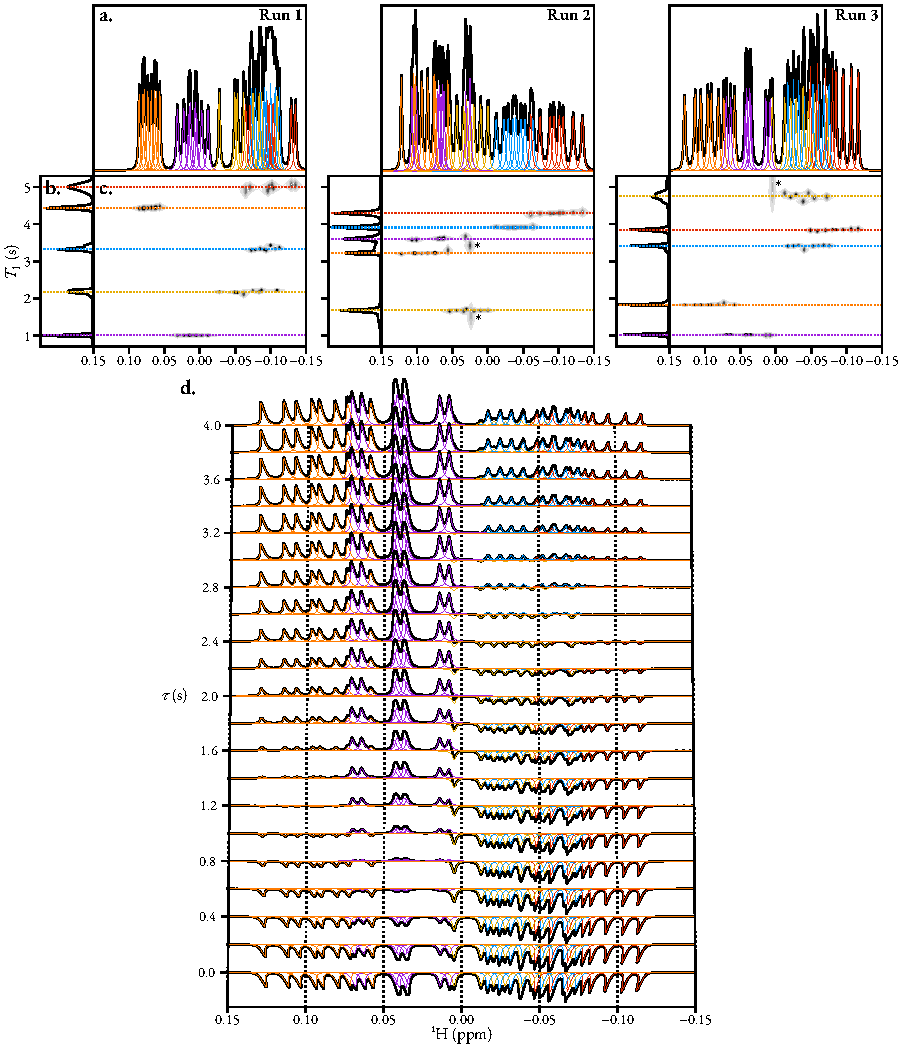
\includegraphics{five_multiplets_invrec/five_multiplets_invrec.pdf}
    \caption[
        Three examples of results generated when considering simulated
        inversion recovery datasets comprising five ddd multiplet structures.
    ]
    {
        Three examples of results generated when considering
        simulated inversion recovery datasets comprising five ddd multiplet
        structures.
        \textbf{a.} Plot of the result generated for the first increment ($\tau
        = \qty{0}{\second}$), with all the plots multiplied by $-1$. Black:
        spectrum of the data. Coloured lines: peaks corresponding to
        oscillators in the estimated model. Oscillators with the same colour
        are components of the same multiplet.
        \textbf{b.} Distribution of $T_1$ values, generated
        by projecting the array in panel c onto the $y$-axis.
        \textbf{c.} \ac{DOSY}-style representation of the result, generated using
        \cref{eq:dosy-cross-product},
        with
        $p_{\text{min}} = \qty{0.7}{\second}$,
        $p_{\text{max}} = \qty{5.3}{\second}$,
        $c = 40$,
        $R=128$.
        Dashed horizontal lines denote the true $T_1$ values for each spin.
        \textbf{d.} Estimation result of each increment for Run 3,
        illustrating the evolution of the amplitudes of each oscillator as a
        function of $\tau$.
    }
    \label{fig:five-multiplets-invrec}
\end{figure}
\Cref{fig:five-multiplets-invrec} shows the result achieved by applying the
method outlined in \cref{alg:estimate-seq}
to three simulated inversion recovery datasets featuring 5 overlapping ddd
multiplet structures.
Each dataset was simulated using \textsc{Spinach}, using spin systems which
were defined such that within a
known region of the generated spectrum
(\SIrange{0.15}{-0.15}{\partspermillion}) five ddd
multiplet structures with significant overlap, abiding by the weak coupling
approximation, were present.
Constraints were placed on the shifts and
couplings of the spin system to ensure that no two signals would have
frequencies with a difference less than $\nicefrac{\fswone}{\None}$.
For each spin, a $T_1$ value was sampled from $\mathcal{U}(\qty{1}{\second},
\qty{5}{\second})$, and a $T_2$ value was sampled from
$\mathcal{U}(\qty{0.2}{\second}, \qty{0.6}{\second})$.
Relaxation phenomena were modelled using the ``extended $T_1$/$T_2$
approximation''~\cite{SpinachRelax} (see \cref{subsec:invrec-datasets} for more
information).
Each \ac{FID} generated dataset was corrupted by noise with a target
\ac{SNR} of \qty{40}{\deci\bel}. The \ac{MDL} was used for model order
prediction; it successfully predicted that 40 signals were present on each
occasion.

Despite heavy overlap between peaks, the routine was successful at
assigning each signal in the dataset with a $T_1$ value that closely agreed
with the $T_1$ of the spin giving rise to it (see
\cref{fig:five-multiplets-invrec}.b). As is to be
expected, in scenarios where little overlap existed between signals with
different decay rates, $T_1$ predictions tended to be more accurate, with
smaller associated errors (see for example the purple and orange multiplets in Run 1.
Nevertheless, good estimates could still be obtained in cases of severe
overlap between signals from different spins (see the red, blue and yellow
multiplets in Run 1). Reassuringly, particular oscillators for which the
estimate of $T_1$ was notably far from the true value tended to be associated
with large errors, with examples denoted with an asterisk in
\cref{fig:five-multiplets-invrec}.c.

\subsubsection{Andrographolide Diffusion}
\begin{figure}
    \centering
    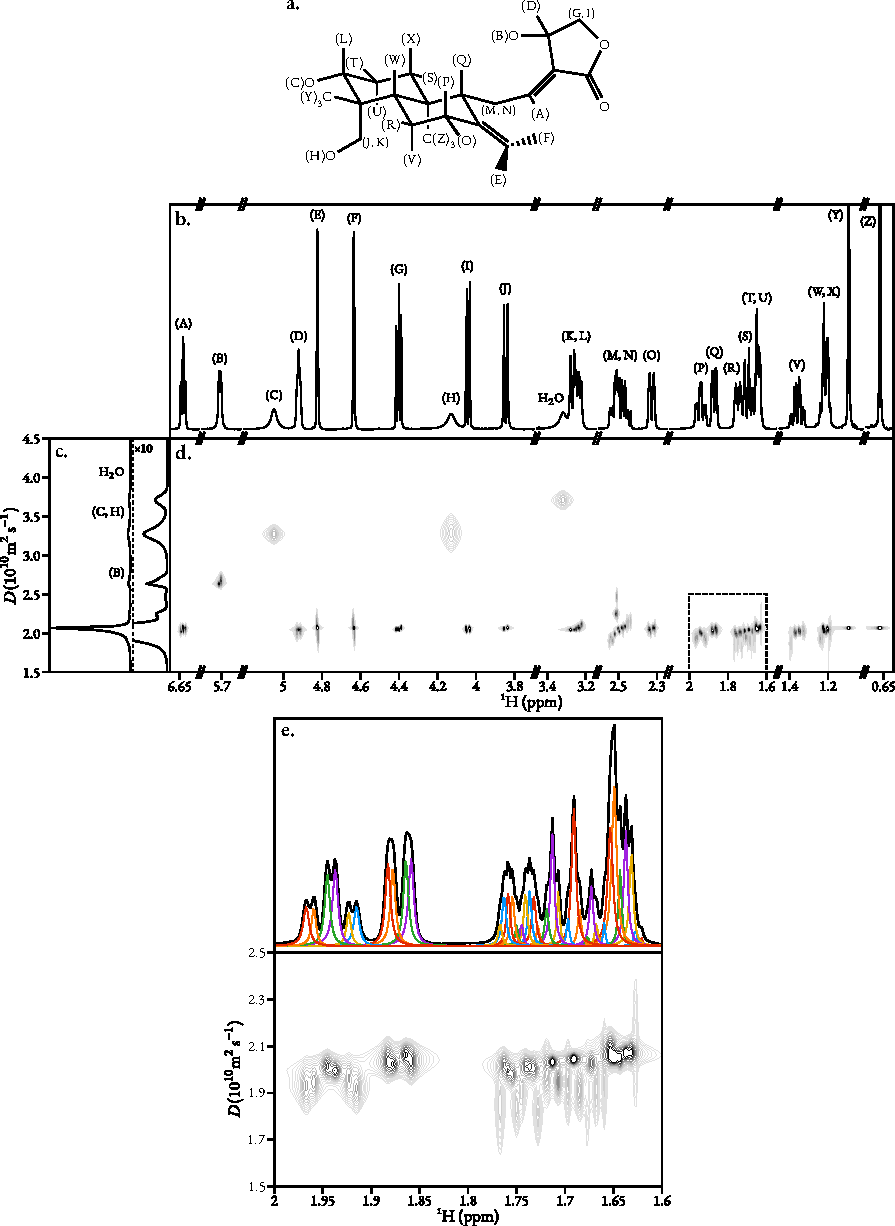
\includegraphics{andrographolide_dosy/andrographolide_dosy.pdf}
    \caption[
        The result of estimating a diffusion dataset of andrographolide.
    ]{
        The result of estimating a diffusion dataset of andrographolide in
        unfresh \acs{DMSOd6}.
        \textbf{a.} Structure of andrographolide.
        \textbf{b.} \ac{1D} spectrum.
        \textbf{c.} Diffusion profile obtained by projecting the contour plot in
        c onto the $y$-axis.
        \textbf{d.} Contour plot mapping estimated oscillators to diffusion constants, with
        $p_{\text{min}} = \qty{1.5e-10}{\meter\squared\per\second}$,
        $p_{\text{max}} = \qty{4.5e-10}{\meter\squared\per\second}$,
        $c = 2.5$,
        $R=128$.
        \textbf{e.} Magnified view of the \SIrange{2}{1.6}{\partspermillion}
        spectral range (see the dashed box in panel d) with estimated
        oscillator peaks plotted.
    }
    \label{fig:andrographolide-dosy}
\end{figure}
\Cref{fig:andrographolide-dosy} shows the result of applying the
estimation technique on a oneshot \ac{DOSY} dataset of andrographolide in
unfresh \acs{DMSOd6} at \qty{298}{\kelvin}. Exposure of the sample to water is
evidenced by the broad
peak around \qty{3.3}{\partspermillion}, estimated to have a diffusion constant
of \qty{3.7e-10}{\meter\squared\per\second}. On top of this, the acidic
hydroxyl protons (B, C, H) of andrographolide show significant line-broadening,
and their estimated diffusion coefficients are considerably different compared
with those of the non-hydroxyl protons, due chemical exchange with water in the
sample~\cite{Chen1998}.
The diffusion profile generated suggests a diffusion constant of andrographolide of
\qty{2.07e-10}{\meter\squared\per\second}. The predicted diffusion constants for
each estimated oscillator, especially those with greater intensity, show
good consistency.
Lower intensity oscillators, especially those which
significantly overlap with others, tended to be associated with
less consistent diffusion constants and larger errors with examples of this
phenomenon apparent in \cref{fig:andrographolide-dosy}.d. A few
oscillators also show a
significant deviation at around \qty{2.5}{\partspermillion}. This is due to the
presence of a 1:2:3:2:1 quintet from partially protonated \acs{DMSO}, due to
proton exchange with the residual water\footnote{
    This multiplet structure arises from the \ch{^1H} in \acs{DMSO} coupling to
    two
    equivalent spin-$1$ \ch{^2H} nuclei. The relative amplitudes of the signals
    can be deduced by considering the ``trinomial triangle'', an extension of
    the more familiar Pascal's triangle, the latter being applicable to
    couplings involving equivalent spin-$\nicefrac{1}{2}$ nuclei.
}. As the
data are insufficiently resolved to enable the separation of andrographoilde and
\acs{DMSO} signals, oscillators exist in the model which have amplitude profiles
influenced by both species, leading to an aggregated diffusion constant. As
$D_{\text{DMSO}} > D_{\text{andrographoilide}}$, the affected oscillators
possess larger predicted diffusion constants.

\subsubsection{Glucose/Valine/Threonine Diffusion}
\begin{figure}
    \centering
    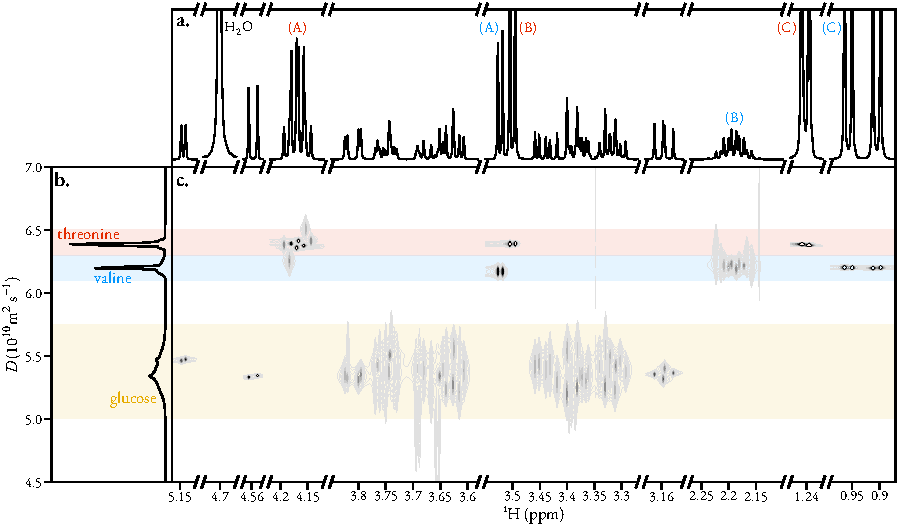
\includegraphics{glu_thre_val_diffusion/glu_thre_val_diffusion.pdf}
    \caption[
        The result of estimating a diffusion dataset for a mixture of L-threonine,
        L-valine and D-(+)-glucose.
    ]{
        The result of estimating a diffusion dataset for a mixture of L-threonine,
        L-valine and D-(+)-glucose in D\textsubscript{2}O.
        \textbf{a.} Structure of L-valine.
        \textbf{b.} Structure of L-threonine.
        \textbf{c1.} Structure of \textalpha-D-glucopyroanose.
        \textbf{c2.} Structure of \textbeta-D-glucopyroanose.
        \textbf{d.} \acs{1D} spectrum, taken from the first \acs{FID} of the
        diffusion dataset.
        \textbf{e.} Diffusion coefficient distribution.
        \textbf{f.} \acs{DOSY}-style plot of chemical shifts vs diffusion
        constant, generated using \cref{eq:distribution}, with
        $p_{\text{min}} = \qty{4.5e-10}{\meter\squared\per\second}$,
        $p_{\text{max}} = \qty{7e-10}{\meter\squared\per\second}$,
        $R=256$, and $c=1.5$.
    }
    \label{fig:gluc_val_thre}
\end{figure}
Another diffusion example is provided by \cref{fig:gluc_val_thre}, where the
estimation routine was applied to a dataset derived from a sample comprising
the molecules L-valine ($M_r = \qty{117.148}{\gram\per\mole}$),
L-threonine ($M_r = \qty{119.120}{\gram\per\mole}$), and D-(+)-glucose ($M_r =
\qty{180.156}{\gram\per\mole}$) dissolved in
D\textsubscript{2}O at \qty{298}{\kelvin}. Not included in the figure is the
result for the water signal, for which a diffusion constant of
\qty{1.88e-9}{\meter\squared\per\second} was determined. The routine
was able to separate of the three species in the sample along the diffusion
axis. Predicted diffusion coefficients for valine and threonine were
\qty{6.20e-10}{\meter\squared\per\second} and
\qty{6.39e-10}{\meter\squared\per\second}, respectively. For glucose, the situation is
complicated by the presence of two major anomeric forms:
\textalpha-D-glucopyroanose and
\textbeta-D-glucopyroanose\footnote{
    The equilibrium mixture in water comprises 38\% of the \textalpha\ isomer
    and 62\% of the \textbeta\ isomer.
    This is evidenced by the
    spectrum in \cref{fig:gluc_val_thre}.a, where the relative integrals of
    the doublets at \qty{5.15}{\partspermillion} and
    \qty{4.56}{\partspermillion} agree with this ratio.
    A tiny amount of the open-chain form will
    also be present, though in a negligible quantity.
}~\cite[Chapter 3]{Davis2002}.
There is some evidence of separation of these anomers, principally due
to the downfield doublets at \qty{5.15}{\partspermillion} (\textalpha-anomer) and
\qty{4.56}{\partspermillion} (\textbeta-anomer), which have estimated diffusion
coefficients of \qty{5.47e-10}{\meter\squared\per\second}
and \qty{5.34e-10}{\meter\squared\per\second}, respectively. Beyond these
however, the other estimated oscillators corresponding to glucose have
associated errors which are too large for clear resolution of the two species.
\correction{
    The small difference in diffusion constants associated with the anomers is
    likely related to how effectively they are able to hydrogen-bond to the
    solvent.
}\label{corr:gluc-D}

As is to be expected, signals which are of greater intensity, and which are
more clearly resolved, enable the determination of diffusion coefficients with
smaller associated errors. A clear example of this behaviour can be recognised when
considering the valine result (see the area shaded blue in
\cref{fig:gluc_val_thre}.c). The
oscillators which lead to diffusion constants with the lowest errors correspond to
the high intensity doublet of doublets around \qty{0.95}{\partspermillion},
resulting from six equivalent protons from two methyl groups. Far
greater uncertainty is observed for the predictions associated with proton (B),
which has a doublet of septets structure, featuring many low-intensity signals.
Similar arguments can be made for the signals which correspond to the other
species in the mixture.
Application of multivariate methods on the dataset was unsuccessful at
extracting diffusion information for the separate components; both
\ac{DECRA} and \ac{SCORE} could extract the water
signal from the rest of the dataset, with the two components having associated
diffusion coefficients of \qty{6.31e-10}{\meter\squared\per\second} (an
aggregate of the valine, threonine, and glucose signals) and
\qty{1.88e-9}{\meter\squared\per\second}, respectively.

\section{Ideal Spectra from Single-Chirp Excitation}
\label{sec:bbqchili}
There are numerous nuclei of interest in \ac{NMR} with very wide chemical shift
ranges, including \ch{^{19}F} (of particular interest in the pharmaceutical
industry), \ch{^{31}P}, and \ch{^{195}Pt}.
Attaining spectra covering the entire chemical shift range of such nuclei for
use in quantitative applications is challenging due to off-resonance effects,
which severely alter the amplitudes and phases of resonances with frequencies
far from that of the transmitter\cite[Section 3.4.1]{Cavanagh2007}. One
popular means of achieving ultra-broadband excitation, in which a consistent
amplitude- and phase-profile across a spectral window of tens or even hundreds
of \unit{\kilo\hertz} the achieved, is to use \ac{FS} pulses, during
which the frequency of \ac{RF} irradiation varies with
time\cite{Foroozandeh2020}. One of the most common classes of \ac{FS} pulses
are those where the variation of excitation frequency with time is linear, with
such pulses commonly referred to as \emph{chirp} pulses. The application of a
single \ang{90} chirp pulse to achieve ultra-broadband excitation, while
involving a simple and short pulse sequence, yields
spectra with undesirable phase behaviour, on account of resonances with
different frequencies being excited at different moments in time.
There are well-established methods for overcoming this using
pulse sequences featuring an initial excitation, followed by one or more
refocussing \ac{FS}
pulses\cite{Bohlen1989,Bohlen1993,Cano2002,Power2016,Foroozandeh2019}.

With knowledge of the form of the chirp pulse, the expected phase of a
particular signal is determinable, and in this section, it will be shown
that well-phased spectra can be obtained from excitation with a single \ac{FS}
pulse when appropriate post-processing of the \ac{FID} is employed.
The main advantage of being able to derive spectra with desirable features from
a single chirp excitation experiment is the fact that ultra-broadband spectra
can be generated using with a far shorter pulse sequence than state of the art
methods such as \ac{CHORUS}\cite{Power2016,Foroozandeh2019}, where both a
\ang{90} chirp pulse, and two \ang{180} chirp pulses are applied; spectra with
improved signal intensity could therefore be realised. Here, a description of the
technique is presented, followed by an illustration of its performance on both a
simulated and an experimental dataset.

\subsection{Chirp Excitation}
\begin{figure}
    \centering
    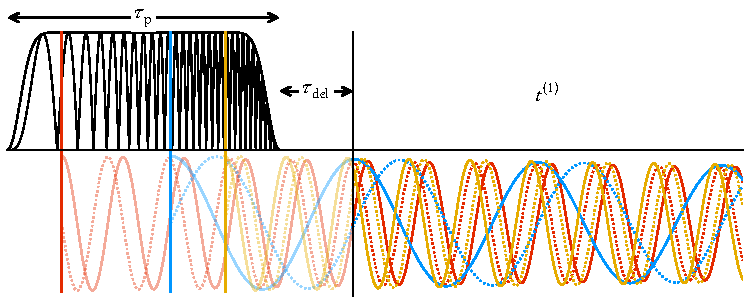
\includegraphics{single_chirp_illustration/single_chirp_illustration.pdf}
    \caption[
        An illustration of an experiment comprising a single chirp pulse.
    ]
    {
        An illustration of an experiment comprising a single chirp pulse sweeping
        low to high frequencies of duration $\tau_{\text{p}}$, followed by
        a pre-scan delay period of time $\tau_{\text{del}}$, prior to
        acquisition. The fate of three resonances with different frequencies is
        denoted, with $f_{\text{red}} < f_{\text{blue}} <
        f_{\text{yellow}}$. Each resonance is excited at different points
        in time, with lower frequency resonances being excited earlier, such that
        each of these evolves for different amounts of time prior
        to acquisition ($\tau_0$).
        The resulting \ac{FID} comprises signals whose phases depend on their
        frequencies quadratically.
        Coloured oscillations denote the evolution of each resonance, with
        solid and dashed lines representing real and imaginary components,
        respectively. It is assumed that the pulse rotates each
        resonance so as to be in phase with the receiver at the point of
        excitation.
    }
    \label{fig:single-chirp}
\end{figure}
Focus is limited here to chirp pulses which sweep from low to high
frequencies; the are parameterised by
their duration $\tau_{\text{p}}$ (\unit{\second}),
excitation bandwidth $\Updelta F$ (\unit{\hertz}),
and \ac{RF} ``amplitude'' $\omega_{\text{RF}}$ (\unit{\hertz}).
The frequencies that a pulse sweeps through are in the range
$[\foff - \nicefrac{1}{2} \Updelta F,
\foff + \nicefrac{1}{2} \Updelta F]$,
and the rate at which the frequency of the chirp is increased (the sweep
rate) is given by $\nicefrac{\Updelta F}{\tau_{\text{p}}}$.
\Cref{fig:single-chirp} provides an illustration of a single chirp
excitation experiment. After application of the chirp pulse, there is typically
a short pre-scan delay $\tau_{\text{del}}$, usually on the order of a few
\unit{\micro\second}, prior to the start of acquisition. While the pre-scan
delay can be determined if an intimate knowledge of the spectrometer hardware
is known, this varies from instrument to instrument, and is not trivial to
ascertain. It is this delay which induces a first-order phase shift in \ac{NMR}
experiments, and which is routinely corrected for by phase correction.
The various chirp pulse parameters are inter-related as
follows\cite{Foroozandeh2019,Kupce1995b}:
\begin{equation}
    \omega_{\text{RF}} = \sqrt{
        \frac{\Updelta F Q}{2 \pi \tau_{\text{p}}}
    },
\end{equation}
where $Q \in \mathbb{R}_{>0}$ is the \emph{adiabaticity factor}.
For a pulse with flip angle  $\beta < \ang{180}$, $Q$ is related to $\beta$ via
\begin{equation}
    Q = \frac{2}{\pi} \ln \left( \frac{2}{\cos(\beta) + 1} \right),
\end{equation}
such that an appropriate pulse to achieve a flip angle of \ang{90} requires
selecting a combination of $\omega_{\text{RF}}$, $\Updelta F$, and
$\tau_{\text{p}}$ which satisfies $Q \approx 0.441$.
The combination used in examples in this work are $\Updelta F =
\qty{400}{\kilo\hertz}$, $\tau_{\text{p}} = \qty{100}{\micro\second}$, and
$\omega_{\text{RF}} \approx \qty{16.8}{\kilo\hertz}$.
For a pulse with sufficiently low $\omega_{\text{RF}}$\,---\,this requires a
sufficiently large pulse duration for a given excitation bandwidth\,---\,it is
reasonable to assume that the chirp pulse induces an instantaneous \ang{90}
rotation at the point of resonance, as depicted in
\cref{fig:single-chirp}. As such, resonances with different
Larmor frequencies evolve for different amounts of time prior to the start of
acquisition, according to
\begin{equation}
    \tau_0\left(f\right) =
        \tau_{\text{del}} + \frac{\tau_{\text{p}}}{2} -
        \frac{(f - \foff) \tau_{\text{p}}}{2 \Updelta F}.
    \label{eq:t0}
\end{equation}
$\tau_{\text{del}} + \nicefrac{\tau_{\text{p}}}{2}$ is the amount of time
between excitation and detection for the on-resonance case, in which
excitation occurs exactly halfway through the pulse. Resonances
with a frequency smaller than that of the transmitter are excited earlier and hence
have a larger $\tau_0$, while the converse is true for resonances with greater
frequencies. The resulting overall phase as of a signal a function of its
frequency can be approximated as\cite{Foroozandeh2019}
\begin{equation}
    \phi(f) = \phi_0 + 2 \pi \left(\tau_{\text{del}} + \frac{\tau_{\text{p}}}{2} \right) (f - \foff) -
        2 \pi \left(\frac{\tau_{\text{p}}}{2 \Updelta F}\right)
        (f - \foff)^2.
    \label{eq:quadratic-phase}
\end{equation}
One might assume that it is possible to generate phased spectra by simply
applying phase correction to the spectrum generated, via
\begin{equation}
    s_{\phi}(f) = s(f) \exp(-\iu \phi(f)).
        \label{eq:spec-phase-chili}
\end{equation}
While the quadratic phase behaviour of peaks is corrected by doing this,
another issue with the dataset is not addressed;
for any resonance, the signal that is detected can be thought of as
the difference between two signals:
\begin{enumerate}
    \item The ``complete'' signal, which starts at the time of excitation.
    \item A ``truncated'' signal which is identical to the complete signal
        before acquisition, and which comprises zeros once acquisition has
        begun.
\end{enumerate}
The linear nature of the \ac{FT} dictates that the
resulting delayed-acquisition spectrum comprises the difference between the
\acp{FT} of the complete signal and the truncated signal.  The \ac{FT} of a
severely
truncated \ac{FID} comprises a broad sinc function with its maximum
at the signal frequency. The appearance of the sinc wiggle depends on
the gap between excitation and acquisition; resonances of lower
frequencies will exhibit deeper, narrower artefacts since the signal is more
significantly truncated. The result of applying quadratic phase correction is
therefore a spectrum of well-phased peaks, but with major baseline distortions,
particularly in the low-frequency region. Figures \ref{fig:bbqchili-sim}.b and
\ref{fig:bbqchili-real}.b both provide examples of this phenomenon.

\subsection{Methodology}
Both the quadratic phase behaviour and delay-induced baseline distortions can
be resolved if an estimate of the \ac{FID}'s parameters is obtained. This enables
the construction of a synthetic \ac{FID} featuring oscillators which are
back-propagated, such that they begin not at the point of acquisition, but at
the point of excitation. The appropriate start time for an oscillator with
frequency $f$ is given by $-\tau_0$, with $\tau_0$ defined in \cref{eq:t0}. The
resulting corrected \ac{FID} $\by \in \mathbb{C}^N$ is defined as
\begin{equation}
    y_n = \sum_{m=1}^{M} \amexpphim \exp((2 \pi \iu (f_m - \foff) - \eta_m) (n \Dt - \tau_0(f_m)))\quad
        \forall n \in \lbrace 0, \cdots, N-1 \rbrace.
    \label{eq:backprop}
\end{equation}
This concept has similarities to the use of \ac{LP} in order to back-propagate
an \ac{FID} to correct for corrupted initial points. However, a holistic
approach such as \ac{LP} cannot be used in this application, as each signal
component must be treated differently according to its frequency.

Thus far in this work, it has been assumed that all signals which make up a
dataset are of the same phase. Of course this isn't the case for \acp{FID}
generated from single-chirp excitation. As such, it is inappropriate to
incorporate the variance of oscillator phases in the fidelity for \ac{NLP}.
For the examples presented in this section, \ac{NLP} was not applied at all;
the direct output of the \ac{MPM} was used as the estimate of the \acp{FID}
parameters.

\subsection{Results}
\begin{figure}
    \centering
    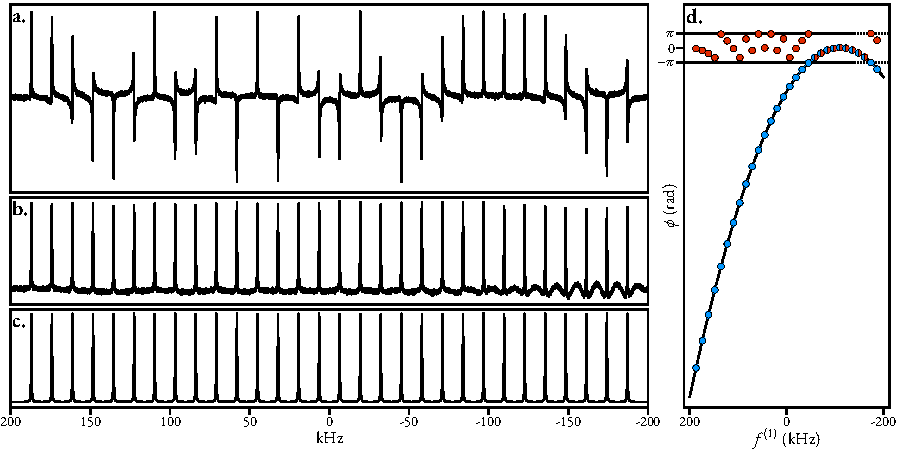
\includegraphics{chirp_phase_vs_estimation/chirp_phase_vs_estimation.pdf}
    \caption[
        A comparison of quadratic phase correction vs frequency-dependent
        back-propagation in treating simulated single-chirp excitation data.
    ]
    {
        A comparison of quadratic phase correction vs frequency-dependent
        back-propagation in treating simulated single-chirp excitation data.
        \textbf{a.} Simulated spectrum for a spin system comprising 30 spins
        with uniformly-separated resonance frequencies. The data was generated
        with
        $N=2^{14}$,
        $\fsw=\qty{400}{\kilo\hertz}$,
        $\foff=\qty{0}{\hertz}$,
        $\tau_{\text{p}} = \qty{100}{\micro\second}$,
        $\tau_{\text{del}} = \qty{0}{\second}$,
        $\Updelta F = \qty{400}{\kilo\hertz}$.
        Coloured lines depict individual oscillators generated using the
        \ac{MPM}; these have been slightly offset for clarity.
        \textbf{b.} Spectrum generated using quadratic phase correction
        (\cref{eq:spec-phase-chili}).
        \textbf{c.} Spectrum generated using the back-propagation approach.
        \textbf{d.} Estimated phases of each oscillator as a function of
        frequency. Red points: phases wrapped within the range $(-\pi, \pi]$.
        Blue points: the same phases, adjusted by addition of a suitable multiple
        of $2 \pi$ to each red point in order to display their quadratic
        dependence on frequency.
        Black curve: quadratic fit of the blue points. The equation of the
        quadratic is stated.
    }
    \label{fig:bbqchili-sim}
\end{figure}
\Cref{fig:bbqchili-sim,fig:bbqchili-real} present comparisons
between the application of quadratic phase correction and the proposed
back-propagation procedure. In the former, a simulated
dataset is considered, comprising 30 evenly-spaced signals, and generated using
\cref{eq:backprop} with $-\tau_0(f_m)$ replaced with $+\tau_0(f_m)$. Other
relevant parameters used are stated in the caption.
A very large damping factor ($\qty{1000}{\per\second}$) was assigned to each
oscillator, as this augments the baseline distortions in the spectrum.
\ac{AWGN} was added to the \ac{FID}, with a target \ac{SNR} of
\qty{25}{\deci\bel}.

The spectrum after quadratic phase correction (\cref{fig:bbqchili-sim}.b)
exhibits the undesired baseline distortions as discussed, with more intense,
narrower baseline distortions associated with lower-frequency signals.
The \ac{MPM} was used to estimate the \ac{FID}'s parameters,
with only the first 2048 points considered
Performing the \ac{MPM} on a signal with $2^{14}$ points would take (a) a
long time, and (b) require a very large amount of \ac{RAM} (see Figures
\ref{fig:mpm-profiling}.a1 and \ref{fig:mpm-profiling}.a2).
Estimating a truncated \ac{FID} comprising the first 2048 points of the
data is justifiable here, since all signal frequencies are spaced
reasonably far apart, meaning each signal in the \ac{FID} becomes
resolvable from the others early on into evolution.
The spectrum generated via back-propagation is presented in
\cref{fig:bbqchili-sim}.c, which is well-phased, and does not suffer from
severe baseline distortion. The variation of the estimated oscillator
phases against their frequencies is plotted in \cref{fig:bbqchili-sim}.d, with
the quadratic dependence clearly illustrated; fitting the blue points to a
quadratic function yielded a second-order coefficient of
$\qty{-7.85e-10}{\radian\second\squared}$, in agreement with the expected value
of $-2 \pi \left(\nicefrac{\tau_{\text{p}}}{2 \Updelta F}\right)$.

\Cref{fig:bbqchili-real} features an experimental dataset, acquired
from a sample of 1\% \ch{Gd}-doped \ch{H2O} in \ch{D2O}\footnote{
    The paramagnetic species \ch{Gd^{III}} is a popular
    contrast agent used in \ac{MRI}, owing to its ability to decrease the $T_1$
    of nearby spins. This typically has an influence on $T_2$ too, with it
    being shortened at high enough concentrations.
    The signal from \ch{H2O} therefore decays at a more rapid rate, such that
    the baseline distortions observed in the phased spectrum of
    \cref{fig:bbqchili-real}.b are more pronounced.
}.
The dataset was acquired using a \ac{2D} experiment, in which the transmitter
offset was adjusted in each increment. The resulting dataset was a series of
\acp{FID}, each comprising a single \ch{H2O} signal with differing frequencies.
When summed, these produce an \ac{FID} with multiple signals at frequencies
defined the selections of transmitter frequencies. The resulting spectrum is
presented in \cref{fig:bbqchili-real}.a.

To produce the phased spectrum in \cref{fig:bbqchili-real}.b, only the
second-order phase was automatically corrected; afterwards, manual
first-order phase correction was applied to the spectrum. This was done
because, as stated above, the
length of the spectrometer delay $\tau_{\text{del}}$ is not trivial to
determine. As with the simulated case, severe baseline distortions exist in the
spectrum, making it unsuitable for quantitative applications.
Analogously, to generate the spectrum via back-propagation, only the
contribution to $\tau_0$ which is dependent on the signal frequency was
included, i.e. $\tau_0$ in \cref{eq:backprop} was replaced with
\begin{equation}
    \tau_{0}^{\prime} = -\frac{(f - \foff) \tau_{\text{p}}}{2 \Delta F}.
\end{equation}
First-order phase correction was then applied to the spectrum produced from the
back-propagated \ac{FID} to yield the result presented in
\cref{fig:bbqchili-real}.c.
In comparison with the quadratic phase-correction approach, it is evident that
a far cleaner spectral baseline is achieved. The phases are not perfectly
consistent across all signals; most notably, the highest- and
second-lowest-frequency signals have phases which stray noticeably from
\ang{0}; it is likely that this resulted from error associated with the
\ac{MPM}. Regardless, it is undeniable that the spectrum produced by
back-propagation achieves a far more desirable result relative to the quadratic
phasing approach.

\begin{figure}
    \centering
    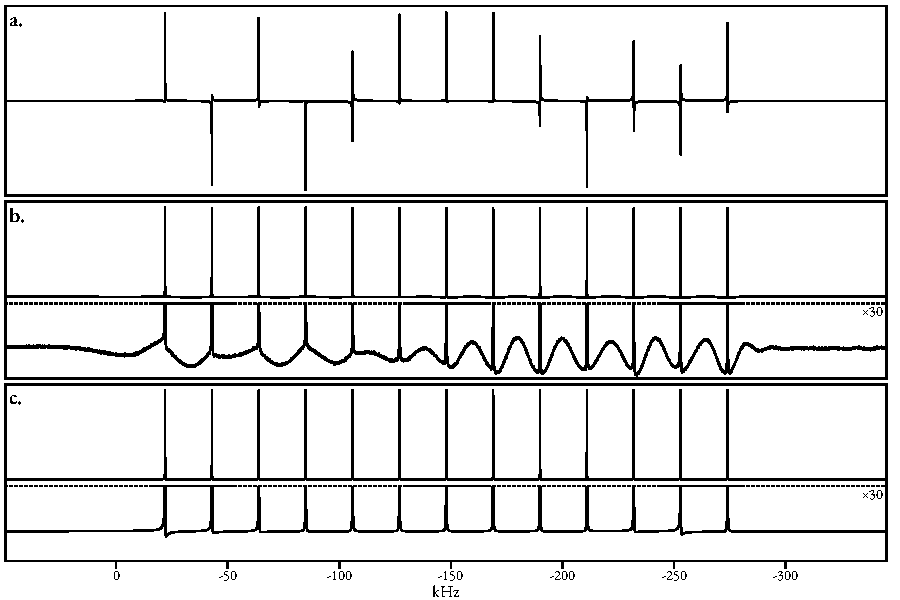
\includegraphics{chirp_phase_vs_estimation_real_data/chirp_phase_vs_estimation_real_data.pdf}
    \caption[
        A comparison of quadratic phase correction vs frequency-dependent
        back-propagation in treating experimental single-chirp excitation data
        generated from a sample of Gd-doped H\textsubscript{2}O in
        D\textsubscript{2}O.
    ]{
        A comparison of quadratic phase correction vs frequency-dependent
        back-propagation in treating experimental single-chirp excitation data
        generated from a sample of 1\% Gd-doped H\textsubscript{2}O in
        D\textsubscript{2}O.
        \textbf{a.} Spectrum generated directly from the acquired \ac{FID}.
        \textbf{b.} Spectrum generated using quadratic phase correction.
        \textbf{c.} Spectrum generated using the back-propagation approach.
    }
    \label{fig:bbqchili-real}
\end{figure}

\section{Summary}

In this chapter, numerous results have been presented, all of which feature
\ac{1D} \ac{FID} estimation.
In \cref{sec:evaluation}, it was illustrated that extending the \ac{MPM}, with
the added step of a phase variance-regularised \ac{NLP} routine, can
aid in the generation of parameter estimates which agree better with the
underlying assumptions of the data structure. Oscillators in the \ac{MPM} often
possess spurious phases; this feature can frequently be rectified by the
\ac{NLP} method. Beyond simply providing a description of the signals which
make up a dataset, it has been shown that parametric estimation can be applied
to further useful ends; two such examples have been presented in
\cref{sec:seq,sec:bbqchili}, respectively.

There are scenarios in which \ac{1D} estimation can perform admirably,
enhancing the information accessible to a spectroscopist. However,
\ac{1D} datasets are typically the most challenging form of \ac{NMR} data to
estimate due to their inherent complexity; with all information about a
sample being distilled into a single dimension, it is very common
(particularly with \ch{^{1}H} datasets) for \acp{FID} to be so densely
populated with signals that extracting meaningful information at
the per-signal level is futile.
\correction{
    It should therefore be appreciated that estimation methods such as the one
    presented in this work\,---\,requiring little to no prior knowledge about
    the dataset to operate\,---\,can only be applied effectively to a limited
    set of cases.
}\label{corr:limited-scope}

Through the separation of signals into more than one detection dimension,
multidimensional experiments can yield datasets which have sufficiently
well-resolved signals for estimation to be applicable to a wider range of
samples. The \ac{2DJ} experiment is such an example, and the estimation of
datasets acquired using it is the focus of the next chapter.


\chapter{2DJ Estimation for Pure Shift NMR}
\label{chap:cupid}
Two key features of the \ac{NMR} experiment for which improvements are
constantly being sought are sensitivity and resolving power.
\correction{
    \label{corr:ns}
    There are numerous means of enhancing sensitivity, such as the use of
    magnets with higher field strengths ($\operatorname{SNR} \propto
    B_0^{3/2}$)~\cite{Maeda2019} and cryogenic probes~\cite{Kovacs2020}, as
    well as simply increasing the number of transients ($\operatorname{SNR}
    \propto N_{\text{t}}^{1/2}$)~\cite[Section 5.2]{Levitt2007}.
}
However, few means of achieving better resolution exist beyond increased field
strengths (resolution $\propto B_0$), and ensuring that a magnetic
field with a high degree of homogeneity is used through the use of shimming.
Significant interest has therefore
been given to the development of techniques which generate broadband homodecoupled
(\emph{pure shift}) spectra, in which the effects of homonuclear scalar
couplings are absent from the data. While often valuable for structural
assignment purposes, the influence of scalar couplings can lead to spectra
which are too crowded for meaningful insights to be gleaned. While it is
commonplace to decouple heteronuclear couplings at the point of \ac{FID}
acquisition~\cite{Shaka1983a, Shaka1983b,Shaka1985}, homonuclear decoupling is
far more challenging. At the time of writing, there are a number of approaches
for acquiring pure shift spectra; the most popular modern approach
involves running a suitable \ac{2D} pulse sequence, and concatenating the initial
sections of each \ac{FID}, in a process referred to as
\emph{chunking}~\cite{Meyer2013,Adams2014,Zangger2015}. The key drawback of all of
these techniques is that the resultant pure shift signal is considerably less
sensitive relative to a standard pulse-acquire experiment, since only a
fraction of the available spin magnetisation contributes to that which is
incorporated into the dataset.

In this chapter, a method for deriving pure shift spectra indirectly via the
estimation of \ac{2DJ} datasets is presented, which has been named
\acfi{CUPID}. It is illustrated that by extracting the parameters which
describe a \ac{2DJ} dataset, a pure shift spectrum with desirable
absorption-mode lineshapes can be produced without the signal loss associated
with experimental pure shift methods.

\section{Pure Shift \acs{NMR}}

In this section, a survey of some of the most prominent procedures for
producing pure shift spectra are presented.

\subsection{The \acs{2DJ} Experiment}
The \ac{2DJ} experiment\cite{Aue1976, Morris2009} provided the first means of
achieving pure shift spectra. It has a simple pulse sequence:
\[
    \ang{90} \xrightarrow{\nicefrac{\tone}{2}} \ang{180} \xrightarrow{\nicefrac{\tone}{2}} \ttwo.
\]
After excitation of magnetisation onto the transverse plane, the indirect
dimension evolution consists of a spin echo, with acquisition following
immediately afterwards. Fourier transformation in both dimensions leads to a
spectrum in which only scalar couplings contribute in $\Fone$, as the chemical
shifts are refocussed by the spin echo, while both scalar couplings and
chemical shifts contribute in $\Ftwo$.  \Iac{FID} generated by the \ac{2DJ}
experiment is hypercomplex, taking the form of \cref{eq:general-fid} with
$D=2$ and $\zeta^{(1)} = \exp(\iu\cdot)$, i.e.
\begin{equation}%
    \begin{split}%
        y_{\none,\ntwo} =
        &\sum_{m=1}^{M} a_m \exp(\iu \phi_m)
            \exp\left(\left(2 \pi \iu \fonem - \etaonem\right) \none \Dtone\right) \times \\
        &\exp\left(\left(2 \pi \iu  \left(\ftwom - \foff\right)
            - \etatwom\right) \ntwo \Dttwo\right)
            + w_{\none,\ntwo}.
    \end{split}%
    \label{eq:jres-fid}
\end{equation}%
The transmitter offset term has been neglected in the indirect dimension, since
chemical shift evolution does not occur.
For each signal in the \ac{FID}, the indirect- and direct-dimension
frequencies are intimately linked. Consider a \ac{2DJ} dataset generated by a
spin system with $S$ distinct spins. The signals giving rise to a particular
spin $s \in \lbrace 1, \cdots, S \rbrace$ form a grouping $G_s
\subset \lbrace 1, \cdots, M \rbrace$. All of the signals in $G_s$
have (angular) frequencies given by
\begin{subequations}
    \begin{gather}
        2 \pi \fonem = \Updelta \omega_m,\\
        2 \pi \ftwom = \omega_{0,s} + \Updelta \omega_m,
    \end{gather}
    \label{eq:f1-f2-2dj}
\end{subequations}
$\forall m \in G_s$, where $\omega_{0,s}$ is the Larmor frequency of
the spin, and $\Updelta \omega_m$ is the displacement
of the signal from $\omega_{0,s}$, as a result of J-couplings\footnote{
    $\Updelta \omega_m$ will be a linear combination of all the scalar
    couplings associated with the spin giving rise to the signal, with all the
    coefficients being $\pm \nicefrac{1}{2}$.
}. Due to the relationship between the direct- and indirect-dimension
frequencies, all signals which are part of the same multiplet lie along
a line which bisects (i.e. makes a \ang{45} angle with) both the $\Fone$ and
$\Ftwo$ axes, as depicted in \cref{fig:jres_spectrum}.a.
\begin{figure}%
    \centering%
    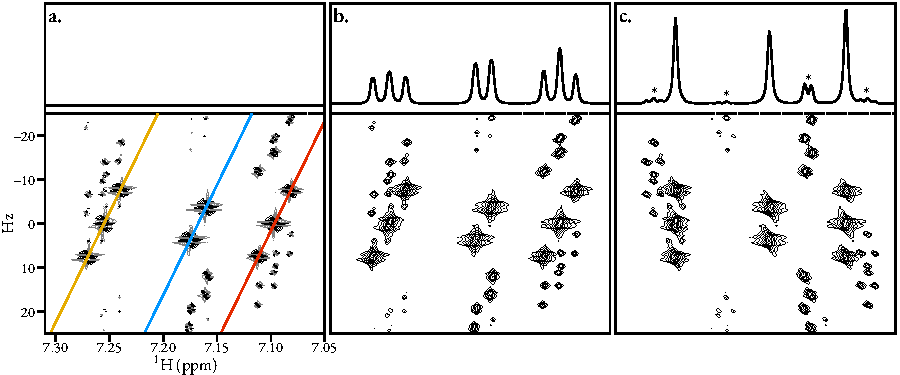
\includegraphics{jres_spectrum/jres_spectrum_new.pdf}%
    \caption[
        Region of a \acs{2DJ} spectrum of strychnine.
    ]
    {%
        Region of a simulated \acs{2DJ} spectrum of strychnine.
        Each panel depicts the spectrum following different processing
        procedures. Below: contour plots of the spectrum. Above: the
        summation of the spectrum along the indirect ($y$) axis.
        \textbf{a.} Spectrum produced by applying sine-bell apodisation
        followed by \ac{FT} in both dimensions.
        Coloured lines denote \ang{45} cross-sections along which the present
        multiplet structures lie.
        \textbf{b.} Magnitude-mode spectrum.
        \textbf{c.} Spectrum generated after application of a \ang{45} shear on
        the magnitude-mode spectrum. Peaks marked with asterisks panel c arise
        from the presence of strong coupling artefacts.
   }%
    \label{fig:jres_spectrum}%
\end{figure}%

One limitation of the \ac{2DJ} experiment is the fact that
spectra with pure absorption lineshapes cannot be produced. This is since, due
to the absence of a mixing period, it is not possible to produce a
complementary pair of phase- or amplitude-modulated \acp{FID}, which are
required to nullify dispersive contributions (see
\cref{subsec:mulitdim}).
The FT of a \ac{2DJ} \ac{FID} produces a spectrum with phase-twist
peaks (\cref{fig:jres_spectrum}.a). As with other experiments which
produce hypercomplex signals, such as \ac{COSY}, the data is conventionally
displayed in ``magnitude-mode'' (\cref{fig:jres_spectrum}.b) in which the
absolute value of each point in the spectrum is plotted.
A pure shift spectrum is generated from the \ac{2DJ} spectrum by performing a
\ang{45} shear\,---\,often referred to as a tilt\,---\,on the spectrum array,
leading to the separation of chemical shifts and scalar couplings onto
orthogonal axes (\cref{fig:jres_spectrum}.c). Each slice through the
direct dimension of the \ac{2DJ} spectrum is subjected to a right circular
rotation such that
\begin{subequations}
    \begin{gather}
        s_{\none,\ntwo}^{\text{tilt}} =
            s_{\none,n^{(2)\prime}},\\
        n^{(2)\prime} = \left(\ntwo + \left\lfloor
                \frac
                    {\fswone \Ntwo\vpsub{\mathrm{sw}}}
                    {\fswtwo \None\vpsub{\mathrm{sw}}}
                \left(
                    \frac{\None\vpsub{\mathrm{sw}}}{2} - \none
                \right)
            \right\rceil
        \right) \bmod \Ntwo.
    \end{gather}
\end{subequations}
This achieves the mapping $s\left(\Fone,\Ftwo\right) \rightarrow s(\Fone, \Ftwo
- \Fone)$, which leads to a spectrum in which all peaks arising from a
given spin reside at the same direct-dimension frequency. The
effectiveness of the shear is maximised when both $\nicefrac{\fswtwo}{\fswone}$
and $\nicefrac{\Ntwo}{\None}$ are powers of 2\note{check this}. Summing the
sheared spectrum along $\Fone$ leads to the pure shift spectrum.
If the spectrum wasn't in magnitude-mode, shearing and summing would lead to
the absorptive and dispersive components of the spectrum cancelling each other
out, such that a vector of noise would be obtained.
With a magnitude-mode spectrum, the process leads to undesirable pure shift
spectra with broad ``wings'' on account of the presence of dispersive
character, and non-linearities. These effects can be suppressed by appropriate
processing to make the FID envelope symmetric in both dimensions, such as with
sine-bell apodisation or pseudo-echo reshaping\cite{Bax1981}, though this
results in a significant reduction in sensitivity being incurred, along with
distortions in relative peak amplitudes.

Another feature which limits the effectiveness of the \ac{2DJ} experiment to
produce pure shift spectra are
\emph{strong coupling artefacts}\footnote{
    As stressed in \cite{Thrippleton2005}, these are not strictly artefacts,
    but rather genuine signals, which are expected to be present in the
    \ac{2DJ} dataset. Despite this, the term is widespread in the literature.
},
which arise due to mixing effects induced by the \ang{180} pulse in the
\ac{2DJ} sequence\cite{Wider1983,Thrippleton2005}. Examples of these are seen
in the spectra of \cref{fig:jres_spectrum}, on account of the three spins
giving rise to the signals seen being strongly coupled. These artefacts always
have direct-dimension frequencies which match those of the conventional signals
in the spectrum\,---\,a feature which will be exploited in the \ac{CUPID}
procedure\,---\,however they do not lie along the same \ang{45} cross
sections. As a result, the final spectrum produced by shearing and summing will
feature extra low intensity signals that do not agree with the chemical shift
of a particular spin (see peaks marked with asterisks in
\cref{fig:jres_spectrum}.c).

\subsection{The \acl{ZS} Method}
\label{subsec:ZS}
Zangger and Sterk introduced a pulse sequence element which achieves
\emph{slice-selective excitation}, by applying a low \ac{RF} power \ang{180}
pulse\footnote{Conventionally, a R-SNOB pulse is used\cite{Kupce1995}.} in the
presence of a \ac{PFG} along the $z$-axis\cite{Zangger1997}. Such an element
excites a
given spin only in a narrow range of heights in the sample, as the \ac{PFG}
induces a shift in resonance frequency according to $\Updelta \omega(z) = \gamma
gz$, where $g$ is the magnitude of the \ac{PFG}. By placing a hard
\ang{180} pulse adjacent to the selective pulse, the
``active'' spin in a given slice is rotated by \ang{360} (i.e. no net
rotation), while all other (``passive'') spins are only rotated by \ang{180}.
Placing such a element in the middle of the $\tone$ evolution therefore
achieves refocussing of the J-couplings associated with the active
spin\cite{Aguilar2010}. In order to achieve effective decoupling of any given
pair of spins, it is necessary that the bandwidth of the selective π-pulse is
smaller than the difference in their Larmor frequencies. However, with more
selective pulses, a smaller proportion of the available spin magnetisation will
contribute to the final FID, and hence sensitivity will be diminished
\footnote{
    The reduction in sensitivity is $\propto \nicefrac{\Updelta F}{\gamma g l_z}$,
    where $\Updelta F$ is the selective pulse bandwidth, and $l_z$ is the length of
    the sample lying within the receiver coil ($\approx
    \qty{1.5}{\centi\meter}$).
}.
Therefore a trade-off exists between effective decoupling of all spins, and
achieving the greatest sensitivity possible. In the case of strong coupling,
the \ac{ZS} method tends to perform poorly relative to other options for this
reason. The \ac{ZS} element has been utilised in order to generate \ac{2DJ}
datasets comprising phase-modulated pairs, enabling the generation of pure
absorption-mode spectra\cite{Pell2007}. Pure shift spectra with far more
desirable lineshapes can be achieved relative to using a typical magnitude-mode
spectrum \ac{2DJ}, though with a significant loss of sensitivity.

\subsection{The \acs{BIRD} Method}
The \ac{BIRD} pulse sequence element\cite{Garbow1982,Bax1983} also takes
advantage of the idea of selectively inverting passive spins, while leaving
active spins unaffected.
However the active spins are those which are directly bound to a low natural
abundance
heteronucleus, with the two most common heteronuclei used being
\textsuperscript{13}C (1.1\% abundance) and \textsuperscript{15}N (0.37\%
abundance).
The passive spins are those bound to far more abundant nucleus (i.e.
\textsuperscript{12}C or \textsuperscript{14}N). The reduction in sensitivity
of the experiment relative to a full-sensitivity experiment is therefore known
and constant across samples. In scenarios where strong coupling exists, \ac{BIRD} can
achieve improved sensitivity over \ac{ZS}, since with the latter a very weak
selective pulse would be required to ensure it is of a sufficiently small
bandwidth. The \ac{BIRD} method is particularly attractive in scenarios where
the sensitivity penalty due to the involvement of a low-abundance nucleus has
already been paid, for example in sequences where an \ac{INEPT} element is
present\cite{Paudel2013}. One of \ac{BIRD}'s primary drawbacks is the fact that
geminal protons (i.e. protons bound to the same heteroatom) cannot be decoupled
from each other, since such protons are always in the same subset of either
active or inactive nuclei. Doublets rather than singlets will arise in such
cases.

\subsection{\acs{PSYCHE}}
\label{subsec:psyche}
The most recent major development in pure shift spectroscopy is the \ac{PSYCHE}
experiment\cite{Foroozandeh2014,Foroozandeh2018}.
\note{Description... Element, How it works (very simple), Effectiveness}

With \ac{PSYCHE}, the proportion of active and passive spins is
dependent on the flip angle of the chirp pulses; for a
\ac{PSYCHE} element featuring chirp pulses with flip angles $\beta$, the
proportions of are $\cos^2 \beta$ and $\sin^2 \beta$, respectively.

The \ac{PSYCHE} element has also been employed in conjunction with the \ac{2DJ}
experiment in order to produce spectra which already feature orthogonal
separation of the chemical shifts and couplings along the two frequency
axes\cite{Foroozandeh2015,Kiraly2017}. Being a 3D experiment, the
\ac{PSYCHE}-\ac{2DJ} requires long experiment times (typically tens of hours)
in order to produce a spectrum with well-resolved multiplet structures in the
indirect dimension.

\subsection{Pure shift spectra from 2DJ estimation}
\note{Mandelstahm?}

Beyond specialised pulse sequences, procedures based on the estimation of
\ac{2DJ} datasets have also been developed to achieve broadband homodecoupling.
Nuzillard introduced \ac{ALPESTRE}\cite{Nuzillard1996,Martinez2012}, in which
the parameters of each indirect-dimension FID are estimated using \ac{LPSVD},
such that a set of parameters $\symbf{\Theta} \in \mathbb{R}^{\Ntwo
\times 4M}$ is generated.
\begin{equation}
    \symbf{\theta}_{\ntwo} =
    \begin{bmatrix}
        \bda_{\ntwo}\T &
        \bdphi_{\ntwo}\T &
        \bdf_{\ntwo}\T &
        \bdeta_{\ntwo}\T
    \end{bmatrix}\T.
\end{equation}
The parameters generated are used to propagate each FID backward into
$-\tone$, producing a ``full-echo'':
\begin{equation}
    \begin{split}
        y^{\text{full}}_{\none,\ntwo} = \sum_{m=1}^{M}
            a_{\ntwo,m}
            \exp(\iu \phi_{\ntwo,m})
            \exp\left(\left(2 \pi \iu f_{\ntwo,m} \none
            -\eta_{\ntwo,m}  \left\lvert \none \right\rvert \right)\Dtone\right), \\
        \forall \none \in \lbrace -\None + 1, \cdots, 0, \cdots, \None - 1 \rbrace,\ \forall \ntwo \lbrace 0, \cdots, \Ntwo - 1 \rbrace.
    \end{split}
    \label{eq:full-echo}
\end{equation}
\ac{FT} of \cref{eq:full-echo} generates a spectrum whose real component
comprises absorption-mode
Lorentzian character in both dimensions. This opens up the means of producing
pure-shift spectra from the \ac{2DJ} experiment with sharp lineshapes and
without signal loss. A similar approach proposed by Mutzenhardt et al.
instead constructs full echoes via \ac{LP} of each direct-dimension
\ac{FID}, and generates a full echo by propagating into
$-\ttwo$\cite{Mutzenhardt1999}.



\section{Methodology}
\ac{CUPID}, a new method developed for pure shift \ac{NMR}, fits into the category
of techniques which utilise \ac{2DJ} estimation. In this section, a description
of it is given.

\subsection{The Estimation Routine}
Recall the assumption that a \ac{2DJ} \ac{FID} takes the functional form
of \cref{eq:jres-fid} (\cpageref{eq:jres-fid}). The primary steps involved in
estimating a \ac{2DJ} dataset, for a given spectral region of interest, are:
\begin{enumerate}
    \item Generation of a frequency-filtered sub-\ac{FID} corresponding to
        the region of interest (\textit{vide infra}:
        \cref{subsec:jres-filtering}).
    \item Prediction of the sub-\ac{FID}'s model order, either by applying the
        \ac{MDL} on the first increment in the direct dimension\footnote{
            The first increment of a \ac{2DJ} experiment, for which $\tone =
            \qty{0}{\second}$, effectively takes the same form as an \ac{FID}
            derived from a pulse-acquire experiment.
        } (\cref{subsec:model-order}, \cpageref{subsec:model-order}) or
        by manually specifying a value.
    \item Generation of an initial parameter estimate using the \ac{MMEMPM}
        (\cref{subsec:mmempm}, \cpageref{subsec:mmempm}).
    \item Subjection of the initial parameter estimate to phase
        variance-regularised \ac{NLP} (\cref{sec:nlp}, \cpageref{sec:nlp}).
\end{enumerate}
Instead of estimating successive \ac{1D} \acp{FID}, as proposed by
Nuzillard and Mutzenhardt \emph{et~al.}, \ac{2DJ} sub-\acp{FID} are considered
holistically; a number of benefits are realised because of this.
First, multiplet structures which heavily overlap in a
conventional \ac{1D} dataset can become separated in the \ac{2DJ} dataset,
assuming that the Larmor frequencies of the relevant spins are sufficiently
different.
Accurate resolution of the \ac{FID}'s constituent signals in more crowded spectral
regions is far more likely to be successful with a full \ac{2D} estimation as a
result.
On top of this, there is an additional resolution advantage relative to the
estimation of \emph{direct} dimension \ac{1D} \acp{FID}. Due to the presence of a spin
echo during $\tone$, signal damping effects caused by field inhomogeneities are
nullified, such that damping is dictated solely by transverse relaxation
($T_2^{\vphantom{*}}$). However, during $\ttwo$, the influence of field
inhomogeneities is not
corrected, such that damping occurs at a faster rate, characterised by $T_2^*$
(see \cref{fn:t2-star} in \cref{sec:seq}, \cpageref{fn:t2-star}).
As such, multiplet structures in the indirect dimension exhibit better
resolution (assuming $\nicefrac{\fswone}{\None}$ and
$\nicefrac{\fswtwo}{\Ntwo}$ are comparable).
A further benefit comes with having access to the frequencies of
signals in \emph{both} dimensions, since this opens up the opportunity to group
together those which belong to the same multiplet, as will be discussed in
\cref{subsec:mp-selection}.
Similar information can be obtained
by extracting cross-sections of a sheared magnitude-mode \ac{2DJ} spectrum at
appropriate values of $F^{(2)}$, though the lineshapes of peaks suffer from the
undesirable characteristics described above.

As was mentioned in \cref{subsec:model-order} (\cpageref{subsec:model-order})
applying the \ac{MDL} on a \ac{2D} \ac{FID} is time-consuming,
since a complete \ac{SVD} computation on the
very large block-Hankel matrix $\symbf{E}_{\symbf{Y}}$ would need to be
performed.
Assuming that the spectral region being considered is not too
crowded, applying the \ac{MDL} on the first direct-dimension \ac{FID} can
return reasonable estimates of $M$ at a far smaller computational cost. For
particularly crowded regions, resorting to a manual specification of model
order by inspecting the \ac{2DJ} spectrum is the best solution currently
available.
An interesting benefit is sometimes realised when the \ac{1D} \ac{MDL} is
used for model order selection.
As has been discussed above, the presence of strong coupling artefacts in the
\ac{2DJ} dataset leads to additional nuisance peaks appearing in pure shift spectra
produced by the shear-and-project approach. Exactly the
same phenomenon would occur when parametric estimation is employed, assuming
that the strong coupling artefacts are incorporated into the parameter
set. However, since the
artefacts have direct-dimension frequencies which are identical to those of
first-order signals in the dataset, it is incredibly challenging to resolve
these using the \ac{1D} \ac{MDL}. Therefore, the \ac{MDL} is often
found to predict a model order which agrees with the number of first-order
signals, rather than the \emph{true} number of signals in the \ac{FID}. As the
\ac{MMEMPM} generates a parameter estimate based on the $M$ most significant
components of in dataset, the more intense first-order signals are expected to
be quantified, whereas the weaker strong coupling artefacts will be neglected.
It should be noted that this concept is not infallible, though it has been
observed on a number of occasions. There are instances where strong coupling
artefacts are incorporated into the estimation result, either because the
prediction of $M$ was excessive, or certain artefacts possess particularly
large amplitudes; examples of these situations will be seen later.

\subsection{The \ang{-45} Signal}
\begin{figure}
    \centering
    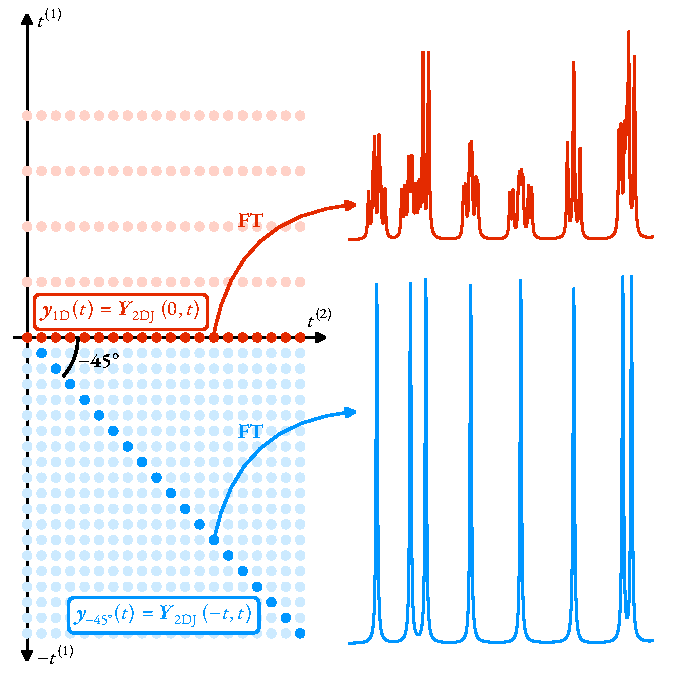
\includegraphics{neg_45_signal/neg_45_signal.pdf}
    \caption[
        The reasoning behind the name ``\ang{-45}
        signal'', which is used to generate pure shift spectra as part of
        \acs{CUPID}.
    ]{
        The reasoning behind the name ``\ang{-45}
        signal'', which is used to generate pure shift spectra as part of
        \ac{CUPID}. The pale red
        dots denote
        a typical \ac{2DJ} \ac{FID}, where
        the amount and rate of sampling in the direct dimension is greater than
        in the indirect dimension (i.e. $\None \ll \Ntwo$ and $\fswone \ll
        \fswtwo$). The bright red dots correspond to the first direct-dimension
        signal $\bY_{\text{2DJ}}(0,\ttwo)$, which has the same form as
        \iac{FID} from a pulse-acquire experiment. A hypothetical signal
        generated by propagating the \ac{FID} into $-\tone$, with the same rate
        of sampling in both dimensions, is denoted with pale blue dots. Taking
        the diagonal of this signal, such that it forms a \ang{-45} angle with the
        $\ttwo$ axis\,---\,the convention of angles being defined through an
        anticlockwise rotation starting on the $\ttwo$-axis has been applied
        here\,---\,yields an \ac{FID}
        $\by_{\ang{-45}}$  which is
        homodecoupled. Note that there is a slight discrepancy
        between \cref{eq:neg-45} and this description, in that the
        indirect dimension damping factors $\bdetaone$ are neglected in the
        former case.
    }
    \label{fig:neg-45}
\end{figure}
The \ac{2DJ} estimation routine yields the parameter vector $\bth \in
\mathbb{R}^{6M}$. With
knowledge of the frequencies and damping factors in both dimensions, it is
possible to generate \iac{FID} which will produce a pure shift spectrum
directly, rather proceeding via the full-echo approach of Nuzillard and
Mutzenhardt \emph{et~al}.
The desired synthetic \ac{FID} produced is named the \emph{\ang{-45} signal}
$\symbf{y}_{\ang{-45}} \in \mathbb{C}^{\Ntwo}$:
\begin{equation}
    y_{\ang{-45},\ntwo} =
        \sum_{m=1}^{M} a_m \exp (\iu \phi_m)
        \exp\left(\left(2 \pi \iu \left(\ftwo_m - \fone_m - \foff\right)
                - \etatwo_m
            \right) \ntwo \Dttwo
        \right),
    \label{eq:neg-45}
\end{equation}
with the reasoning behind the name provided by \cref{fig:neg-45}.
The \ang{-45} signal
takes the form of a conventional \ac{1D} \ac{FID},
except that the frequency of each oscillator, which would be $\ftwo_m$ in a
pulse-acquire experiment,
is replaced with $\ftwo_m - \fone_m$. In the \ang{-45} signal, oscillators
belonging to the same multiplet $s$ will all provide a contribution to the
\ac{FID} with the frequency $f_{0,s}$.
Assuming that the parameters associated with the \ac{2DJ}
\ac{FID} are accurately determined, a pure shift spectrum with sharp
absorption-mode lineshapes and no loss of signal can be generated by this approach.

\subsection{Filtration of \ac{2DJ} Data}
\label{subsec:jres-filtering}
Unlike the direct dimension, which can often comprise sparsely distributed
peaks in the Fourier domain, the indirect dimension of \ac{2DJ} datasets tends
to be densely populated since all multiplet structures are centered at
\qty{0}{\hertz}, and rarely span beyond $\pm \qty{50}{\hertz}$. As such,
the generation of frequency-filtered sub-\acp{FID} is limited to
the direct dimension in \ac{2DJ} estimation.
The filtering procedure applied to \ac{2DJ} data is an extension of that
for \ac{1D} data described in \cref{sec:filtering} (\cpageref{sec:filtering}):
\begin{enumerate}
    \item The array $\symbf{Y}_{\text{VE}} \in \mathbb{C}^{\None \times 2
        \Ntwo}$, is constructed, which contains the \ac{VE} of each
        direct-dimension \ac{FID}, i.e. each row of the array is given by
        \begin{equation}
            \begin{gathered}
            \by_{\text{VE},\none} =
                \begin{bmatrix}
                    \Re\left(y_{n^{(1)}, 0}^{\vphantom{*}}\right) &
                    y_{n^{(1)}, 1}^{\vphantom{*}} &
                    \cdots &
                    y_{n^{(1)}, \Ntwo - 1}^{\vphantom{*}} &
                    0 &
                    y_{n^{(1)}, \Ntwo - 1}^* &
                    \cdots &
                    y_{n^{(1)}, 1}^*
                \end{bmatrix},\\
                \forall n^{(1)} \in \lbrace 0, \cdots, N^{(1)} - 1 \rbrace.
            \end{gathered}
        \end{equation}
    \item $\symbf{Y}_{\text{VE}}$ is subjected to \ac{FT} along the direct
        dimension to produce the spectrum  $\symbf{S}_{\text{VE}}$
        (\cref{fig:jres-filtering}.a); this has an imaginary component of
        zeros.
    \item A super-Gaussian $\symbf{G} \in \mathbb{R}^{\None \times 2 \Ntwo}$ is
        constructed
        (\cref{fig:jres-filtering}.b):
        \begin{equation}
            \symbf{G} = \symbf{1} \otimes \symbf{g}^{(2)},
        \end{equation}
        where $\symbf{1} \in \mathbb{R}^{\None}$ is a vector of ones, and
        $\symbf{g}^{(2)} \in \mathbb{R}^{2\Ntwo}$ is a super-Gaussian vector
        given by \cref{eq:super-Gaussian-onedim}
        (\cpageref{eq:super-Gaussian-onedim}).
    \item A matrix of additive noise is generated by extracting the variance
        $\sigma^2$ of a direct-dimension strip of $\symbf{S}_{\text{VE}}$ which
        is devoid of peaks, and generating an array $\symbf{W}_{\sigma^2} \in
        \mathbb{R}^{\None \times 2 \Ntwo}$ with values independently sampled
        from $\mathcal{N}(0, \sigma^2)$ (\cref{fig:jres-filtering}.c).
    \item The spectrum is filtered (\cref{fig:jres-filtering}.d):
        \begin{equation}
            \widetilde{\symbf{S}}_{\text{VE}} = \symbf{S}_{\text{VE}} \odot
            \symbf{G} + \symbf{W}_{\sigma^2} \odot (\symbf{1} - \symbf{G}).
        \end{equation}
    \item $\widetilde{\symbf{S}}_{\text{VE}}$ is subjected to \ac{IFT} and is
        sliced in half in the direct dimension, yeilding the final filtered
        signal $\widetilde{\symbf{Y}}$.
\end{enumerate}
As with the \ac{1D} case, this method can also be extended to
incorporate spectral slicing, acting to reduce the number of points present in
the filtered sub-\ac{FID}.

\begin{figure}
    \centering
    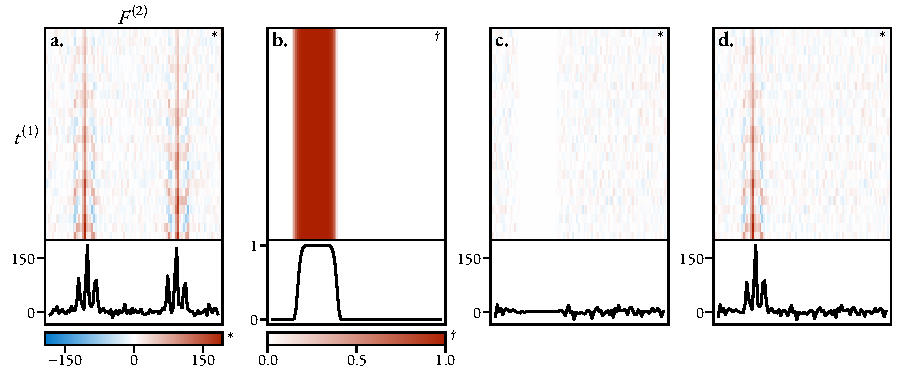
\includegraphics{jres_filtering/jres_filtering.pdf}
    \caption[
        The filtering procedure for \acs{2DJ} data.
    ]
    {
        The filtering procedure for \ac{2DJ} data.
        Each panel consists of a heat-map of the complete \ac{2D} array, as well as
        a plot of the first slice of the array in the direct dimension ($x$-axis).
        \textbf{a.} The spectrum $\symbf{S}_{\text{VE}}$,
        \textbf{b.} Super-Gaussian filter $\symbf{G}$,
        \textbf{c.} Additive noise, attenuated by the super-Gaussian, $\symbf{W}_{\sigma^2} \odot (\symbf{1} - \symbf{G})$,
        \textbf{d.} Filtered spectrum $\widetilde{\symbf{S}}_{\text{VE}}$
        Figures \ref{fig:jres-filtering}.a to \ref{fig:jres-filtering}.d
        are analogous to
        Figures \ref{fig:filtering}.b to \ref{fig:filtering}.e
        for the \ac{1D} case (\cpageref{fig:filtering}).
    }
    \label{fig:jres-filtering}
\end{figure}


\subsection{Multiplet Prediction}
\label{subsec:mp-selection}
\ac{CUPID}'s ability to group oscillators present in a parameter set into
multiplet structures relies on simultaneously knowing both the indirect- and
direct-dimension frequencies of each model oscillator. As has already been
established, for oscillators which are associated with the same multiplet
grouping $G_s$, the quantities $\ftwo_{m_1} - \fone_{m_1}$ and $\ftwo_{m_2} -
\fone_{m_2}$ should be equal ($f{0,s}$) for any pairing  $m_1, m_2 \in
G_s$. An assessment of whether two oscillators belong to the same multiplet can
therefore be made using the following criterion:
\begin{equation}
    \left \lvert
        \left( \ftwo_{m_1} - \fone_{m_1} \right) -
        \left( \ftwo_{m_2} - \fone_{m_2} \right)
    \right \rvert < \epsilon.
\end{equation}
$\epsilon \in \mathbb{R}_{>0}$ is a threshold to account for uncertainty in
the estimation result. A lower bound on $\epsilon$ is the separation between
adjacent points in the better-resolved dimension of the spectrum, i.e.
$\min\left(\nicefrac{\fswone}{\None},
\nicefrac{\fswtwo}{\Ntwo}\right)$.  However, limitations in resolution due to
relaxation-induced signal damping and field inhomogeneities can require
$\epsilon$ to be increased beyond this for effective assignments
to be achieved. \Cref{lst:mp-assign} (\cpageref{lst:mp-assign}) provides a
\Python routine that can be used for multiplet prediction.

There are certain circumstances where it is safe to assume that a
particular oscillator in the estimation result is not associated with a
first-order signal in the dataset;
no oscillator which was derived from a first-order signal will abide by both of
the following:
\begin{enumerate}
    \item The oscillator is not grouped with any other oscillator as part of
        the multiplet assignment.
    \item The magnitude of the indirect dimension frequency of the oscillator
        is appreciably greater than \qty{0}{\hertz}.
\end{enumerate}
If a first-order signal is the only
member of a multiplet grouping, it must be a singlet, and as such it will have
an indirect-dimension frequency of \qty{0}{\hertz}. Oscillators which do agree
with the two points above can be assumed to be related to either strong
coupling artefacts or noise, and can be automatically discarded from the final
parameter estimate.

\correction{
    It is worth mentioning that the procedure of multiplet prediction outlined
    does not naturally allow one to determine the coupling constants associated
    with each spin. With a complete list of the
    frequencies associated with a multiplet structure, the relevant spin's
    coupling network can be predicted. However, it is not guaranteed that the
    estimation routine will extract all frequencies within a multiplet; this is
    particularly so with complex multiplets with significant signal overlap.
    However, it is typically the case that the frequencies extracted by the
    estimation routine can be used as a starting point to manually determine
    the coupling constants.
}\label{corr:coupling-constants}

\section{Results}
\label{subsec:cupid-results}
A number of examples of the application of \ac{CUPID} are now provided.
Initially, a few results are presented on datasets simulated using
\textsc{Spinach}. After this, examples are provided with experimental data. In
a couple of these, comparison of the result acquired using \ac{CUPID} is
made with a spectrum acquired using \ac{PSYCHE}. For details relating to
generation of the datasets, see Sections \ref{sec:simulated-datasets} and
\ref{subsec:cupid-experimental} in the Appendix.

\subsection{``Four Multiplets''}
\label{subsec:four-mp}
\begin{figure}
    \centering
    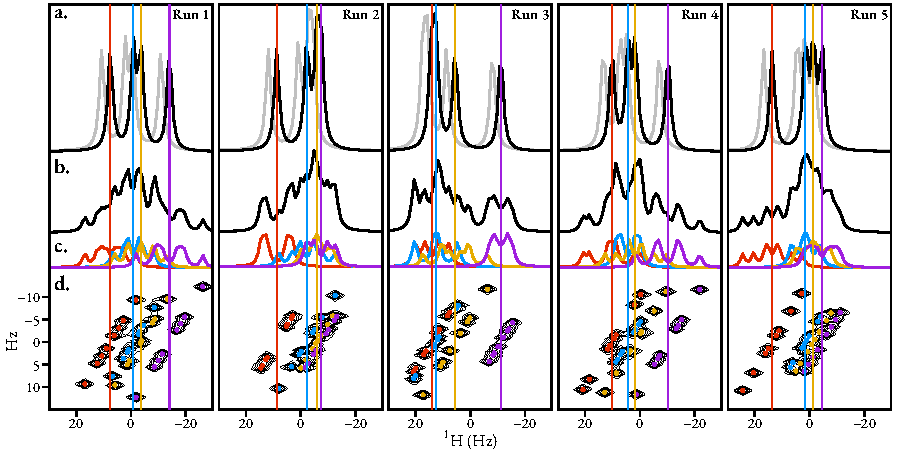
\includegraphics{four_multiplets/four_multiplets}
    \caption[
        The result of applying \acs{CUPID} to 5 instances of simulated
        \acs{2DJ} datasets with 4 heavily overlapping multiplet structures.
    ]{
        The result of applying \ac{CUPID} to 5 instances of simulated \ac{2DJ}
        datasets with 4 heavily overlapping multiplet structures.
        \textbf{a.} Black: pure shift spectrum generated by \ac{CUPID} (via the
        \ang{-45} signal).
        Grey: \ac{1D} spectrum simulated with Spinach, using the same spin
        system as was used to produce the \ac{2DJ} dataset, but with all scalar
        couplings set to \qty{0}{\hertz}. This has been offset slightly for
        clarity.
        \textbf{b.} \ac{1D} spectrum of the dataset, produced using the first
        direct-dimension \ac{FID} in the \ac{2DJ} dataset.
        \textbf{c.} Multiplet structures predicted, using a threshold $\epsilon
        = \nicefrac{\fswtwo}{\Ntwo} \approx \qty{0.98}{\hertz}$.
        \textbf{d.} Contour plot of the \ac{2DJ} spectrum in absolute-value
        mode. Coloured points denote the frequencies of oscillators in the
        estimation result.
        Coloured vertical lines denote the predicted central frequencies of
        each multiplet structure.
    }
    \label{fig:four-multiplets}
\end{figure}
A series of simulated \proton\ \ac{2DJ} datasets were generated such that
within a known region of the spectrum (\SIrange{-30}{30}{\hertz}), four ddd
multiplet structures with significant overlap exist. To achieve this, a
spin-system with 7 spins was formed, with the spins divided into 2 subsets:
\begin{itemize}
    \item Four of the spins (the ``estimated spins'') were assigned random
        resonance frequencies sampled from $\mathcal{U}(\qty{-20}{\hertz},
        \qty{20}{\hertz})$.
    \item The remaining three spins (the ``coupling spins''), were coupled to each
        of the estimated spins, with the values of the couplings randomly
        sampled from $\mathcal{U}(\qty{-10}{\hertz}, \qty{10}{\hertz})$.  The
        coupling spins were given chemical shifts such that they lay far from
        the estimated spins in the spectrum (i.e. their frequencies were $\gg
        \qty{20}{\hertz}$).
\end{itemize}
\ac{AWGN} noise was added to the \ac{FID}, with a target \ac{SNR} of \qty{30}{\deci\bel}.
A filtered sub-\ac{FID} containing only the signals from the estimated spins
was then generated using the filtering procedure described above, with
$l^{(2)}_{\unit{\hertz}} = \qty{30}{\hertz}$,
$r^{(2)}_{\unit{\hertz}} = \qty{-30}{\hertz}$.
The resulting sub-\ac{FID} was expected to comprise 32 ($4 \times
2^3$) oscillators. To assess the estimation procedure's ability, a random
integer from the range $[33, 40]$ was selected as the initial number of
oscillators. Hence, the initial guess from the \ac{MMEMPM} would comprise a
excessive number of oscillators. Due to the severe overlap of the multiplets,
application of the \ac{MDL} on the first direct-dimension signal would be
ineffective and return an under-estimate of the model order. Each \ac{FID} was
subjected to estimation, yielding the result vector $\bthstar$. Spurious
oscillators were checked for, using the criteria outlined above, with the
threshold for multiplet assignment set to the spectral resolution in the direct
dimension: $\epsilon = \nicefrac{f_{\text{sw}}^{(2)}}{\Ntwo}$. If spurious
oscillators were found, these were removed, and \ac{NLP} was run on the updated
set of parameters.

Figure \ref{fig:four-multiplets} illustrates the result achieved for 5 separate
runs of this procedure.
For each \ac{FID} generated, the method was effective at producing an
estimation result with 32 oscillators, as desired, despite the excessive number
that were present in $\bthzero$. Most of the excessive oscillators were purged
from $\bthzero$ through the \ac{NLP} procedure. When spurious oscillators did
remain\footnote{for 2 of the 5 datasets, the result after \ac{NLP} comprised 33
oscillators}, they were then detected when checking for spurious oscillators
and subsequently removed. With simulated examples, it is easy to confirm that
the pure shift spectrum generated using \ac{CUPID} agrees with the expected
pure shift spectrum; it is possible to generate the ``true'' pure shift
spectrum by simulating a pulse-acquire experiment with \textsc{Spinach}, using
a spin system with same chemical shifts, but all scalar couplings set to
\qty{0}{\hertz}.
As seen in panel a of Figure \ref{fig:four-multiplets}, the spectra produced
using \ac{CUPID} agree well with these. Panel c indicates that \ac{CUPID}
effectively resolved the multiplet structures associated with the dataset.

\subsection{Sucrose simulated}
\label{subsec:sucrose-cupid}
\note{Maybe not so impressive? Perhaps try strychnine?}
\begin{figure}
    \centering
    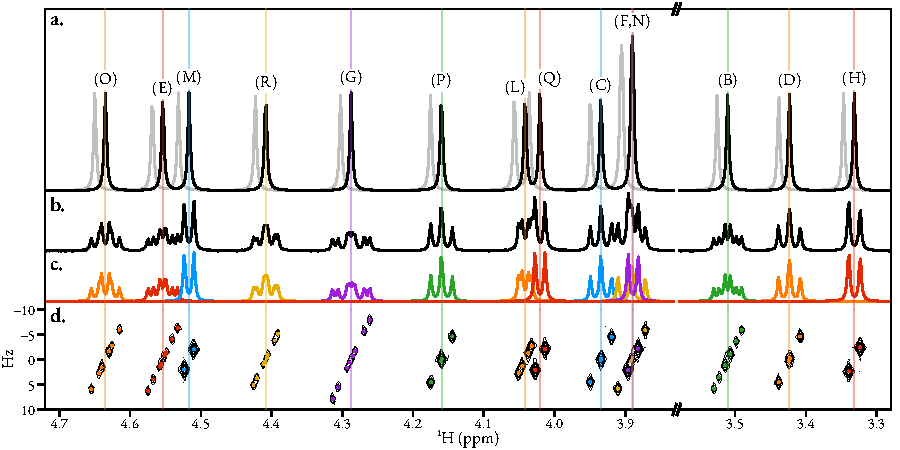
\includegraphics{sucrose_cupid/sucrose_cupid.pdf}
    \caption[
        Application of \acs{CUPID} on a simulated sucrose \acs{2DJ} dataset.
    ]
    {
        Application of \ac{CUPID} on a simulated sucrose \ac{2DJ} dataset.
        \textbf{a.} Black: the spectrum generated from \ac{FT} of the \ang{-45}
        signal. Grey: the spectrum of a simulated dataset with the same
        chemical shifts, with all scalar couplings set to \qty{0}{\hertz}.
        \textbf{b.} Conventional \ac{1D} spectrum.
        \textbf{c.} Multiplet structures assigned ($\epsilon \approx
        \qty{0.27}{\hertz}$).
        \textbf{d.} Contour plot of the absolute value mode \ac{2DJ} spectrum,
        with the locations of assigned oscillators given as coloured points.
    }
    \label{fig:sucrose-cupid}
\end{figure}
As a second example of applying \ac{CUPID} on simulated data, the chemical
shifts and isotropic scalar couplings associated with a
Gaussian\cite{Gaussian03} \ac{DFT} calculation of sucrose in a vacuum
\footnote{
It is well known that isotropic chemical shift calculations using \ac{DFT} are
typically very inaccurate. The resulting spectrum is not typical of sucrose in
the liquid state, though this doesn't really matter for assessing the
performance of \ac{CUPID}.
}
were used to construct a 2DJ dataset. \ac{AWGN} was added with a target
\ac{SNR} of \qty{20}{\deci\bel}. The CUPID procedure was applied to filtered
sub-FIDs such that the signals arising from all 22 spins were considered, though
only the regions of the dataset with the most interesting multiplet structures
are presented in Figure \ref{fig:sucrose-cupid}.

The estimation technique successfully assigned multiplet structures for all 22
multiplets in the dataset, including structures derived from two spins (F \& N)
with a \qty{0.6}{\hertz} difference in resonance frequency, approaching the
spectral resolution in the direct dimension (\qty{0.537}{\hertz}). The
pure-shift spectrum generated via the \ang{-45} signal again showed close
agreement with a 1D spectrum simulated using the same chemical shifts, with
scalar couplings set to \qty{0}{\hertz}. There are particular multiplets where
the number of oscillators fit using the estimation routine was less than the
true number. Examples of this phenomenon are exhibited in the estimates of the
multiplets for spins B \& O, which are both ddd structures. The scalar
couplings involved meant that certain oscillators were
of such similar frequencies that they were separated by significantly less than
the spectral resolution, and thus resolving these was unrealistic. For
example, there are two pairs of peaks in the spin-B multiplet which lie only
\qty{0.085}{\hertz} apart. Under-fitting in this case had a negligible impact
on the final pure shift spectrum. However there are circumstances which will be
seen in the experimental examples below where more blatant cases of under-fitting
lead to the generation of peaks in the pure shift spectrum which are noticeably
broadened.

\subsection{Quinine}
\begin{figure}
    \centering
    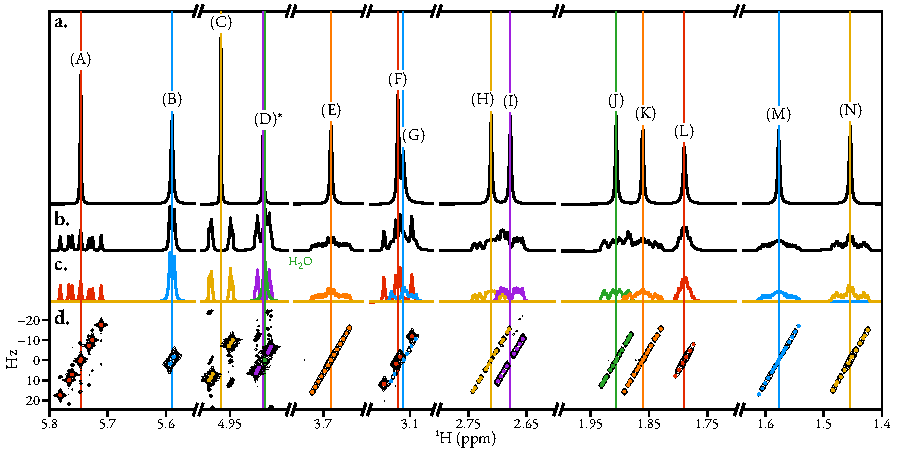
\includegraphics{quinine_cupid/quinine_cupid.pdf}
    \caption[
        Application of \acs{CUPID} on the non-aromatic regions of a quinine
        \acs{2DJ} dataset.
    ]{
        Application of \ac{CUPID} on the non-aromatic regions of a quinine
        \ac{2DJ} dataset.
        \textbf{a.} The spectrum generated from \ac{FT} of the \ang{-45}
        signal, with the signal arising from H\textsubscript{2}O (green, close
        to \qty{4.9}{\partspermillion} neglected).
        \textbf{b.} Spectrum of the first direct-dimension signal in the
        \ac{2DJ} \ac{FID}.
        \textbf{c.} Multiplet structures assigned ($\epsilon =
        \nicefrac{\fswtwo}{\Ntwo} \approx \qty{0.92}{\hertz}$).
        \textbf{d.} Contour plot of the absolute value mode \ac{2DJ} spectrum,
        with the locations of assigned oscillators given as coloured points.
    }
    \label{fig:quinine-cupid}
\end{figure}

Figure \ref{fig:quinine-cupid} illustrates the result of applying \ac{CUPID} on
a dataset generated from a sample comprising quinine (Figure
\ref{fig:structures}.a) in CD\textsubscript{3}OD,
with all signals arising from non-aromatic protons considered. The method
successfully generated a
pure shift spectrum with distinct peaks for each \textsuperscript{1}H
environment. This example also highlights an added benefit of using \ac{CUPID};
it provides the opportunity to suppress ``nuisance'' signals in the pure shift
spectrum. In this
example, an intense, broad singlet at around \qty{4.89}{\partspermillion}
was detected (see the green peak at this frequency in panel c).
The singlet was due to the presence of water in the sample and was a hindrance
due to it overlapping heavily with the multiplet structure corresponding to
spin (D). To obtain a clean singlet for spin (D) in the pure shift spectrum, the
oscillator corresponding to the water signal was simply neglected from
the parameter set used to generate the \ang{-45} signal. This concept of neglecting
nuisance signals through post-processing has been employed extensively, with
the most prominent use case being solvent suppression. The most
significant component in the data (assumed to be the solvent peak), is
determined through \ac{SVD} or some other approach, and is automatically
subtracted from the \ac{FID}\cite{Zhu1997}.
In this case, the water signal is not automatically purged from the parameter
set to construct the final pure shift spectrum, but a knowledgeable user would
be able to locate the water signal, determine that it is undesirable to include
in the pure shift spectrum, and neglect it.


As eluded to already, a few of the peaks in the pure-shift spectrum are rather
broad on account of the estimation routine under-fitting the relevant multiplet
structure. The most notable example of this phenomenon in the quinine example
comes from the peak for spin (G), where close proximity with the spin (F)
multiplet has likely compounded the task of accurately estimating the relevant
oscillators. With fewer oscillators than the true number of contributing signals
fitting a given multiplet structure, the \ac{NLP} routine will compensate by
giving the oscillators it does have at its disposal large amplitudes and
damping factors, so that they can reasonably fit multiple similar-frequency
signals. This behaviour is also exhibited by the multiplet for spin (B),
which comprises two pairs of very close signals in a dd structure. A single
oscillator is fit to each pair of signals, culminating in a broadened pure
shift peak. While linewdiths are affected by under-fitting hard-to-resolve
multiplets, the integrals of the pure shift peaks are not typically perturbed
significantly. \note{COMPUTE INTEGRALS}

\subsection{Camphor}
\begin{figure}%
    \centering%
    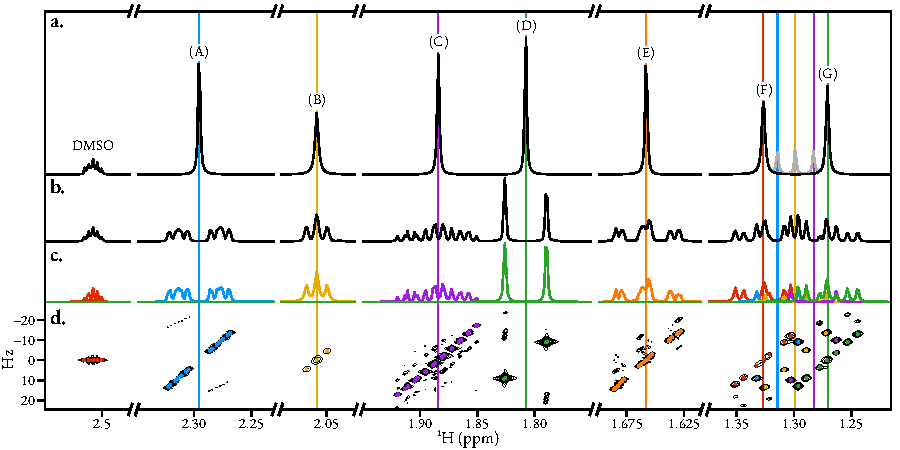
\includegraphics{camphor_cupid/camphor_cupid.pdf}%
    \caption[
        Application of \acs{CUPID} on a camphor dataset.
    ]{
        Application of \acs{CUPID} on camphor \ac{2DJ} dataset.
        \textbf{a.} Black: the spectrum generated from \ac{FT} of the \ang{-45}
        signal. Oscillators associated with strong coupling artefacts between
        spins (F) and (G) were neglected. Grey: spectrum generated without
        neglecting oscillators associated with strong coupling artefacts.
        \textbf{b.} \acs{1D} spectrum produced from the first direct-dimension
        \ac{FID} in the dataset. Note that, unlike a conventional pulse-acquire
        spectrum, strong coupling artefacts are present.
        \textbf{c.} Multiplet structures assigned ($\epsilon =
        \nicefrac{2 \fswtwo}{\Ntwo} \approx \qty{1.23}{\hertz}$).
        \textbf{d.} Contour plot of the absolute value mode \acs{2DJ} spectrum,
        with the locations of assigned oscillators given as coloured points.
    }
    \label{fig:camphor-cupid}%
\end{figure}%
The application of \ac{CUPID} to the non-methyl regions of a \ac{2DJ}
dataset of camphor (Figure \ref{fig:structures}.c) in \acs{DMSOd6} is presented
in Figure \ref{fig:camphor-cupid}. As in the quinine case, there are instances
of underfitting poorly resolved multiplets, resulting in broadened pure shift peaks.
The peak associated with spin (B) is the most drastic case here, where 4
vicinal couplings to protons with dihedral angles of \ang{60} are present,
along with potentially more contributions from long range couplings.
This example highlights the ability of \ac{CUPID} to remove another class of nuisance peak: \emph{strong coupling artefacts}\footnote{
    As stressed in \cite{Thrippleton2005}, these are not strictly artefacts,
    but rather genuine signals, which are expected to be present in the
    \ac{2DJ} dataset. Despite this, the term is widespread in the literature.
},
which arise due to mixing effects induced by the \ang{180} pulse in the
\ac{2DJ} sequence\cite{Thrippleton2005,Wider1983}.
The effects of strong coupling lead to the presence of extra unexpected signals
which do not agree with the chemical shift of any spin associated with camphor.
An example of this is found between \SIrange{1.35}{1.25}{\partspermillion} in
the \ac{2DJ} spectrum, where artefacts associated with spins (F) and (G) are
located.
The estimation routine was able to determine parameters for
the more intense signals which comprise the strong coupling artefacts (these
are coloured blue, yellow, and purple, while oscillators associated with the
true multiplet structures for (F) and (G) are coloured red and green, respectively).
Inclusion of all oscillators extracted by the estimation routine generates the
spectrum in panel a, with the low-intensity grey peaks associated with the strong
coupling effects included. However, in much the same way as the water signal in
the quinine example could be neglected, it is trivial to construct the \ang{-45}
signal with the oscillators associated with strong coupling artefacts left out,
which produces the black spectrum.

\begin{sidewaysfigure}%
    \centering%
    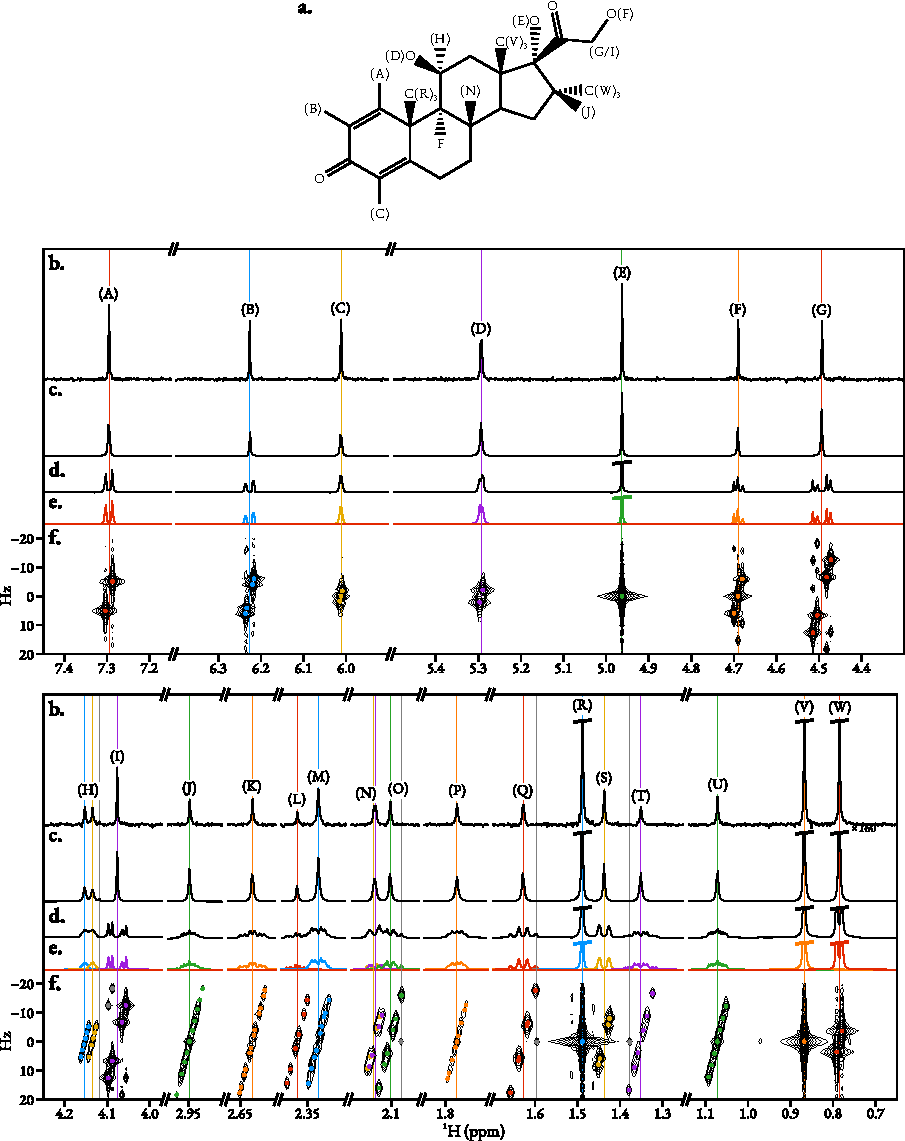
\includegraphics{dexamethasone_cupid/dexamethasone_cupid.pdf}%
    \caption[
        Application of \acs{CUPID} on a dexamethasone dataset.
    ]{
        \note{Fix magnification label.}
        Application of \acs{CUPID} on dexamethasone \ac{2DJ} dataset.
        \textbf{a.} \acs{TSE-PSYCHE} spectrum of the sample.
        \textbf{b.} The spectrum generated from \ac{FT} of the \ang{-45}
        signal.
        \textbf{c.} Conventional \acs{1D} spectrum.
        \textbf{.} Multiplet structures assigned ($\epsilon =
        \nicefrac{\fswtwo}{\Ntwo} \approx \qty{0.92}{\hertz}$).
        \textbf{d.} Contour plot of the absolute value mode \acs{2DJ} spectrum,
        with the locations of assigned oscillators given as coloured points.
    }
    \label{fig:dexamethasone-cupid}%
\end{sidewaysfigure}%
\note{Double check mp thold}

\subsection{Dexamethasone}


Figure \ref{fig:dexamethasone-cupid} shows the result of applying CUPID on a
dataset acquired from a sample dexamethasone in DMSO-d\textsubscript{6}. A
pure-shift spectrum was also acquired using the
\ac{TSE-PSYCHE} experiment\cite{Foroozandeh2018,Foroozandeh2015} for
comparison.
\ac{CUPID} generated a pure-shift spectrum with overall excellent agreement
with the \ac{TSE-PSYCHE} spectrum. Certain multiplet structures in the spectrum exhibit
splitting in the direct dimension, on account of heteronuclear couplings to
\textsuperscript{19}F. Most notable are those derived from spins (D), (H) \& (O). For the (D) multiplet, the
magnitude of the heterocoupling is very small such that assigning these to
separate oscillators was not achievable.
For the spin (N) multiplet, two separate structures were successfully assigned
(see the orange and green multiplets around \qty{2.1}{\partspermillion}).
The estimation routine was unsuccessful at accurately estimating the structure
associated with spin (H), where a severe under-fitting occurred. An under-fitting
of this structure even occurred when the estimation was re-run using
considerable over-estimation of the model order, with most oscillators in the
initial guess being purged during the \ac{NLP} procedure.
The spin (H) multiplet provides an extreme example line-broadening in the pure
shift spectrum on account of under-fitting. The most downfield peaks in the
CUPID spectrum (corresponding to aromatic and hydroxyl protons) also appear to
be noticeably broadened relative to their PSYCHE equivalents. This is also
probably due to under-fitting of the relevant multiplet structures, though to a
far less noticeable extent than for spin H. \note{Any other reason why this
might be so?}

\subsection{Estradiol}
\begin{figure}
    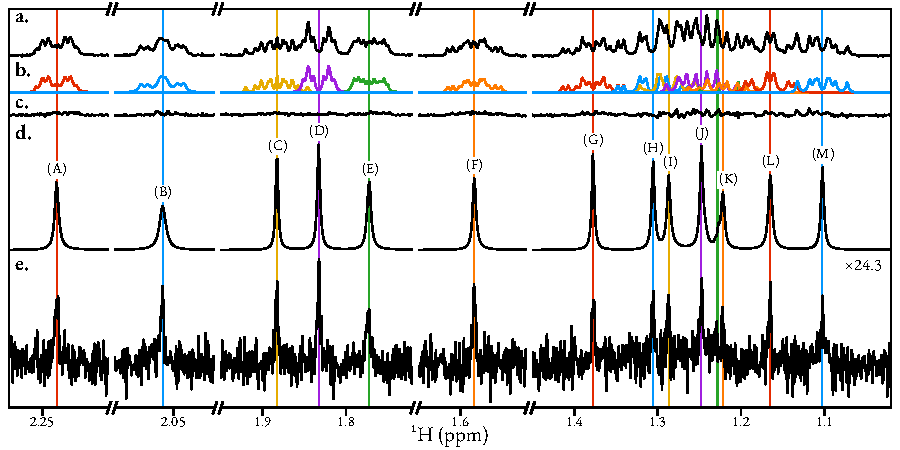
\includegraphics{estradiol_cupid/estradiol_cupid.pdf}%
    \caption[
        Application of \acs{CUPID} on a 17\textbeta-estradiol dataset.
    ]{
        Application of \acs{CUPID} on \ac{2DJ} dataset of 17\textbeta-estradiol
        in \acs{DMSOd6}.
        \textbf{a.} Spectrum of the first direct-dimension \ac{FID} in the
        \ac{2DJ} dataset.
        \textbf{b.} Multiplet structures assigned ($\epsilon =
        \nicefrac{\fswtwo}{\Ntwo} \approx \qty{2}{\hertz}$).
        \textbf{c.} The residual between the spectrum in panel a and the lines
        in panel b.
        \textbf{d.} The pure shift spectrum generated using \ac{CUPID}.
        \textbf{e.} \acs{PSYCHE} spectrum of the sample see Figure
        \ref{fig:psyche} for details on the pulse sequence. The spectrum has
        been scaled such that the maximum is of the same magnitude as the
        corresponding point in the \ac{CUPID} spectrum.
    }
    \label{fig:estradiol-cupid}%
\end{figure}

A final showcase of \ac{CUPID} is provided by Figure \ref{fig:estradiol-cupid}, where a low concentration (\qty{2}{\milli\molar}) sample of 17\textbeta-estradiol (Figure \ref{fig:structures}.

\section{Summary}
In this chapter, \ac{CUPID}, a procedure for the construction of pure shift
spectra via the holistic estimation of \ac{2DJ} datasets, is presented.
Such spectra can be possess myriad beneficial features relative to alternative
methods, albeit with the requirement of a complex post-processing procedure.

% The original method for pure shift spectrum generation consisted of shearing a
% magnitude-mode \ac{2DJ} spectrum by \ang{45}, and computing the projection onto
% the $\Ftwo$ axis. To overcome the grotesque lineshapes which arise due to the
% presence of dispersion character, and non-linearities in the magnitude-mode
% spectrum, severe data treatment such as the used of sine-bell apodisation are
% applied. The resulting pure shift spectra suffer from reduced intensities
% because of this. On top of this, the intensities of peaks are attenuated by
% different extents, such that relative peak integrals become meaningless. The
% presence of strong coupling in the spin system also introduces unwanted
% artefacts into the spectra.

% Experimental procedures  based on ``chunking'' the initial sections of the
% \acp{FID} in a \ac{2D} experiment\,---\,including \ac{ZS}, \ac{BIRD} and
% \ac{PSYCHE}\,---\,have largely superseded the shear and summation approach.
% One key disadvantage of all of these is that only a fraction of the available
% spin magnetisation contributes to the final pure shift spectrum, leading to
% poorer sensitivity.

Through a number of examples, it has been shown that by employing parametric
estimation, a simple \ac{2DJ} experiment can be harnessed to generate pure
shift spectra with sharp absorption Lorentzian peaks which retain the same
signal intensity as the \ac{2DJ} experiment. It it is able to perform
admirably even when state of the art techniques like \ac{PSYCHE} produce
spectra with such low \acp{SNR} as to render them unusable. Frequently, \ac{CUPID}
is able to automatically discard oscillators present in the model which either
correspond to strong coupling artefacts or noise, leading to simplified spectra
which appear to adhere to the weak coupling regime. There are cases where
strong coupling artefacts do end up in the estimation result. It has been shown
that these can be manually neglected from the parameter set so they don't have
an unwanted influence on final pure shift spectrum, though this requires manual
intervention from a knowledgeable user.

Simultaneously, \ac{CUPID} can assign multiplet structures,
by grouping oscillators which lie along a specific \ang{45} cross section in
frequency space. Achieving this experimentally\,---\,effectively involving
a \ac{2DJ} experiment in conjunction with a pure shift element\,---\,requires
running an extremely long (hours or even days) \ac{3D} pulse sequence. The
usefulness of the multiplet structures generated by \ac{CUPID} is dependent on
the level of the estimation routine's accuracy. On
numerous occasions within the examples presented here, the estimation routine
was unable to resolve certain, similar frequency signals. A complete
understanding of the coupling network associated with a given spin in not
attainable when this is so. However, such multiplet structures can still provide
valuable insights into the sample being studied.

\ac{CUPID} is limited by the complexity of the dataset of interest. The reasons
for this are two-fold. First, for datasets comprising progressively more peaks
in a given spectral region, the difficulty in generating effective parameter
estimates becomes harder. Second, with an increased model order required to
estimate the dataset, the time required for computation increases drastically.
This feature is most clearly observed when comparing the times required in
estimating the different regions considered in the estradiol example. As a rule
of thumb, it is anticipated that \ac{CUPID} will perform admirably on datasets
derived from small molecules, though datasets derived from large molecules such
as proteins are likely to be too complex and demanding for good results.


\chapter{Software}
\label{chap:nmrespy}

The estimation routine and applications that have been
presented in the previous three chapters are accessible via the \acfi{EsPy}
package. \ac{EsPy} aims to provide a feature-rich yet simple interface in order
perform estimation on datasets of interest. In this chapter, a short
overview of the package, as well as its accompanying \ac{GUI}, is given.

\section{A description of \acs{EsPy}}

\subsection{Why \textsc{Python}?}
There a number of reasons why \textsc{Python} was the chosen programming
language for \ac{EsPy}:
\begin{itemize}
    \item It has a large user-base, particularly within the scientific
        community.
    \item The \textsc{SciPy} ecosystem~\cite{Virtanen2020}, including the packages
        \textsc{NumPy}~\cite{Harris2020} and
        \textsc{Matplotlib}~\cite{Hunter2007} enables
        high-performance scientific computation and data visualisation in
        \textsc{Python}, despite the language's reputation for slow speed.
    \item Being a scripting language with user-friendly syntax makes
        \textsc{Python} ideal for exploring datasets in a step-by-step fashion.
        This is useful in the context of \ac{EsPy}, as a user will want to
        (a) inspect and pre-process the data of interest,
        (b) determine the regions they wish to estimate and set up the
        estimation routine,
        and (c) output and inspect the result.
        This can be achieved easily by ``hacking'' and re-running
        \textsc{Python} scripts or by using notebook environments, such as
        \textsc{Jupyter}.
    \item It is free and open-source, as opposed to well-known scientific
        computing platforms such as \textsc{Matlab} and \textsc{Mathematica}.
    \item \textsc{Python} supports sophisticated object-oriented programming
        features, including multiple levels of inheritance. This is exploited in
        \ac{EsPy} to facilitate the creation of numerous objects designed with
        specific \ac{NMR} data types in mind (\textit{vide infra}).
\end{itemize}

Probably the largest disadvantage in using \textsc{Python} is its slow performance;
some of the features which makes \Python\ user-friendly lead to significant
runtime overheads\footnote{
    \Python is interpreted rather than compiled, dynamically typed rather
    than statically typed, and it relies on garbage collection for memory
    management, rather than requiring the programmer to do this manually. All
    of these features are slower than the alternatives which are mentioned;
    these alternatives feature in low-level languages like C, C++, and
    \textsc{Rust}.
}. While \textsc{NumPy} provides
interfaces to run fast computations with pre-compiled C-code, a significant
performance benefit would likely be realised if a low-level compiled language
like C, C++, or \textsc{Rust} were used instead (this is discussed more in
\cref{sec:future-work}). While this may be so, the
development time in writing programs with these higher-performance languages is
typically a lot greater those with a higher level of abstraction
like \textsc{Python}.

\subsection{Estimator Objects}
\label{subsec:estimator-objects}
\begin{figure}
    \centering
    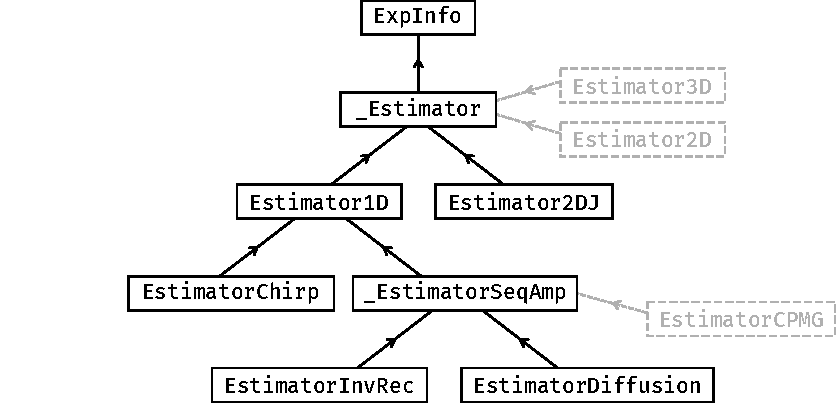
\includegraphics{inheritance_tree/inheritance_tree.pdf}
    \caption[
        An inheritance tree of the estimation classes in the \acs{EsPy} package.
    ]{
        An Inheritance tree of the estimation classes in the \acs{EsPy} package.
        Arrows are directed from child classes to the parent class they
        directly inherit from. Classes in grey are objects that could be added
        to the \ac{API} in the future.
    }
    \label{fig:inheritance}
\end{figure}
The fundamental user-facing objects (\emph{classes}) that \ac{EsPy} provides are
called \emph{estimators}.
Instances of these estimator classes contain relevant pieces of data called
\emph{attributes} (e.g. the \ac{FID} and experiment parameters including the
spectral width and transmitter offset), as well as \emph{methods} which perform
routine applicable to the class like estimation and result figure generation.
Thanks to \textsc{Python}'s support for multiple levels of inheritance, it is
possible to build numerous objects with certain shared attributes and methods,
but which also possess bespoke features that are solely of relevance to
the type of \ac{NMR} data being considered. As an example, only the
\texttt{Estimator2DJ} object possesses a method called \texttt{cupid\_spectrum},
which returns the \ac{FT} of the \ang{-45} signal.
\Cref{fig:inheritance} provides an inheritance
diagram, outlining the relationship between different estimators in
\ac{EsPy}. Basic overviews of each of these are as follows:
\begin{itemize}
    \item \textbf{\textbf{\texttt{ExpInfo}}} stores the parameters that were
        used to run a particular \ac{NMR} experiment. \texttt{ExpInfo} also has
        methods for the generation of the timepoints and chemical shifts sampled
        based on these parameters, and for producing synthetic \acp{FID} if a
        set of signal parameters is provided.
    \item \textbf{\texttt{\_Estimator}} inherits experimental parameters from
        \texttt{ExpInfo}, but also possesses the \ac{NMR} dataset itself.
        This class is designed to contain the functionality which can be
        generalised across all \ac{NMR} data types supported by \ac{EsPy}. It
        does not possess all the features necessary to be useful as a standalone
        object, and as such the user is not supposed to use it directly (such
        an object is often referred to as an abstract class; this is emphasised
        by starting the object's name with an underscore).
    \item \textbf{\texttt{Estimator1D}} handles conventional \ac{1D} datasets,
        such as those in \cref{sec:evaluation}.
    \item \textbf{\texttt{\_EstimatorSeqAmp}} is an abstract class
        which enables the estimation of sequential \ac{1D} datasets such as those
        described in \cref{sec:seq}. Analysis of a given dataset varies depending on
        the type of experiment considered, since the function used for
        fitting amplitudes (\cref{tab:seq-equations}) and the means by
        which that data should be imported varies. As such, this is not
        designed for direct use; one of the classes which inherit it should be
        used instead. Under the hood, \texttt{\_EstimatorSeqAmp} stores a
        number of \texttt{Estimator1D} objects; each of these contains one
        of the \acp{FID} in the sequential dataset. Estimation simply comprises
        iterating through these estimators, giving the parameter estimate of
        the previous estimator to next as its initial guess for \ac{NLP}.
    \item \textbf{\texttt{EstimatorInvRec}} is for the estimation of inversion
        recovery datasets.
    \item \textbf{\texttt{EstimatorDiffusion}} is for the estimation of
        diffusion datasets.
    \item \textbf{\texttt{EstimatorChirp}} is for the estimation of \acp{FID}
        acquired using single-chirp excitation, as described in \cref{sec:bbqchili}.
    \item \textbf{\texttt{Estimator2DJ}} is for the estimation of \ac{2DJ} data.
        This class provides features to generate pure shift spectra and
        assign multiplet structures using \ac{CUPID}, as described in
        \cref{chap:cupid}.
\end{itemize}

Other estimator objects which are yet to be implemented, but are potential
future additions to the package are also depicted in the inheritance diagram.
\texttt{EstimatorCPMG} would enable the analysis of \ac{CPMG}/\ac{PROJECT} datasets,
while \texttt{Estimator2D} and \texttt{Estimator3D} would be
for the estimation of datasets comprising sets of \ac{2D} or \ac{3D} amplitude-
or phase-modulated \acp{FID}, respectively. A discussion of the feasibility of
implementing the \ac{2D} and \ac{3D} estimators is given in
\cref{sec:future-work}.

\subsection{Example Usage}
\mylisting{python3}{code_listings/cupid_example.py}{%
    An example script which makes use of \acs{EsPy}.
}{
    An example script which makes use of the \acs{EsPy} package for the
    consideration of a \ac{2DJ} dataset using \ac{CUPID}.
}{lst:espy-example}
\cref{lst:espy-example} provides an example of \ac{EsPy} being used for the
consideration of \ac{2DJ} data; it is similar to the script which was to
generate the camphor result presented in \cref{fig:camphor-cupid}.  The script
carries out the following:
\begin{enumerate}
    \item An \texttt{Estimator2DJ} object is initialised, which imports and stores
        the \textsc{Bruker}-formatted camphor dataset, located at the path
        \path{$HOME/data/camphor/1}\footnote{
            \path{$HOME} denotes the current user's home directory on a
            UNIX-based system. In many scenarios, the tilde symbol
            (\mintinline{text}{~})
            can be used to denote the home directory as well.
        }
        (Line \ref{ln:newbruker}).
    \item The \ac{2DJ} \ac{FID} is pre-processed to ensure it is phased and
        features a flat spectral baseline (Lines \ref{ln:phase} and
        \ref{ln:baseline}).
    \item The regions of interest are defined, in units of
        \unit{\partspermillion} (Lines \ref{ln:regionstart} to
        \ref{ln:regionend}). Each region is given by a two-element tuple
        containing its left- and right-boundaries.
    \item For each region, parameter estimates are determined using the
        \mintinline{python}{Estimator2D.estimate} method, which constructs a filtered
        sub-\ac{FID}, and subsequently analyses it (Lines
        \ref{ln:estimatestart} to \ref{ln:estimateend}). Most arguments given
        are self-explanatory; \mintinline{python}{nlp_trim} can be set to
        truncate the sub-\ac{FID} in the direct dimension, to reduce the
        computational burden on the \ac{NLP} routine. By default
        the \ac{MDL} is used for model order selection.
    \item After estimation is complete, the estimator object is saved to a byte
        stream using \textsc{Python}'s ``pickling'' protocol~\cite{pickle} (Line
        \ref{ln:pickle}).
        This enables the estimator to be recovered at a later time.
    \item A pure shift spectrum is produced via the \ang{-45} signal, and
        stored to the path \path{$HOME/data/camphor/2} in a format that enables
        it to be read by software that supports \textsc{Bruker} datasets,
        such as \textsc{TopSpin} (Line \ref{ln:writecupid}).
    \item Finally, a figure depicting the estimation result is produced (making
        use \textsc{Matplotlib}) and saved (Lines \ref{ln:makefig} and
        \ref{ln:savefig}). The form the figure takes is reminiscent of
        \cref{fig:camphor-cupid}, though a lot of aesthetic customisation has
        been applied to the latter.
\end{enumerate}

\section{The \acs{EsPy} \acs{GUI}}
\begin{figure}
    \centering
    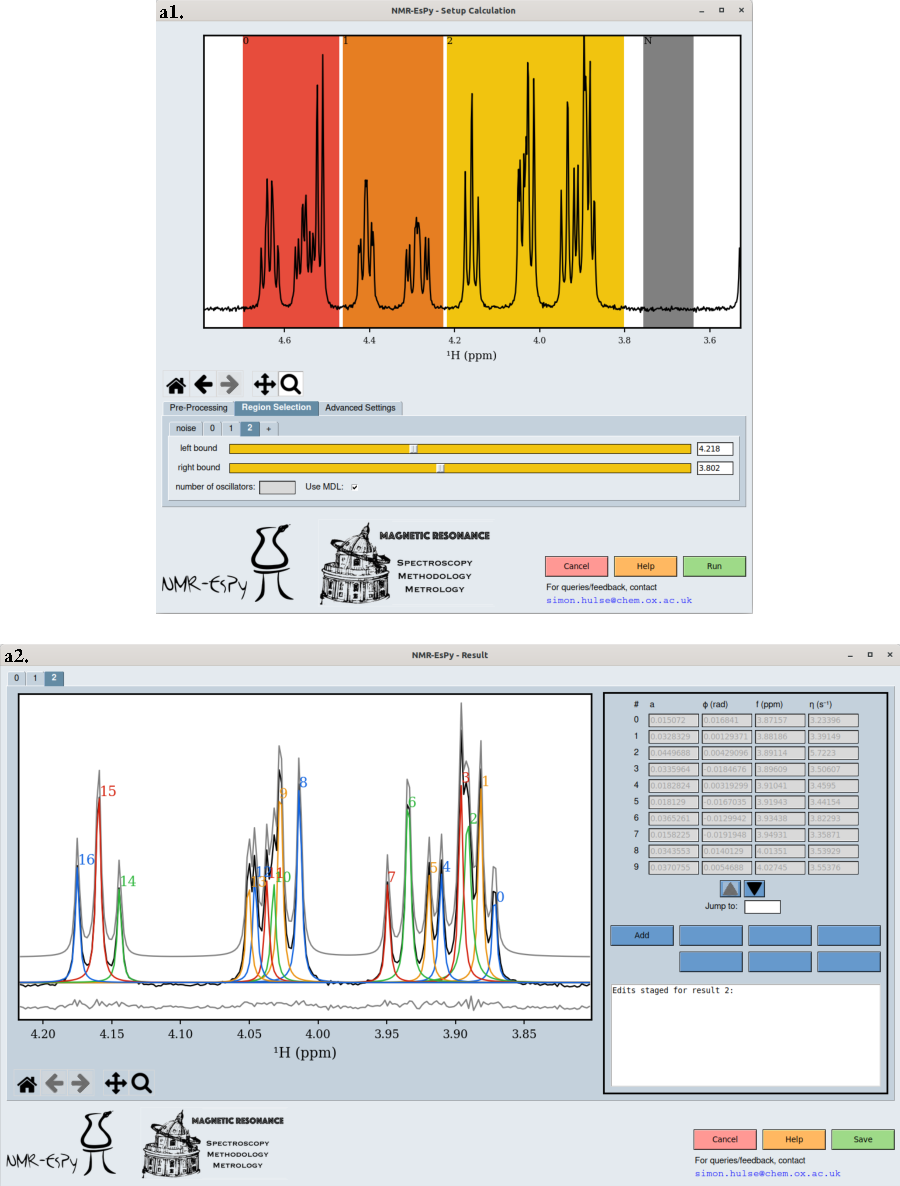
\includegraphics{gui/gui_1d.pdf}
    \caption[
        Screenshots of the \acs{EsPy} \acs{GUI} for \ac{1D} and \acs{2DJ} estimation.
    ]{
        Screenshots of windows that form part of the \ac{EsPy} \ac{GUI} for
        \ac{1D} estimation (\textbf{a.}) and \ac{2DJ} estimation (\textbf{b.}).
        For both data types, the windows used to setup the estimation routine
        (\textbf{1.}) and inspect the result (\textbf{2.}) are shown.
        (Continues on the next page)
    }
    \label{fig:gui}
\end{figure}
\begin{figure}%
    \ContinuedFloat
    \centering
    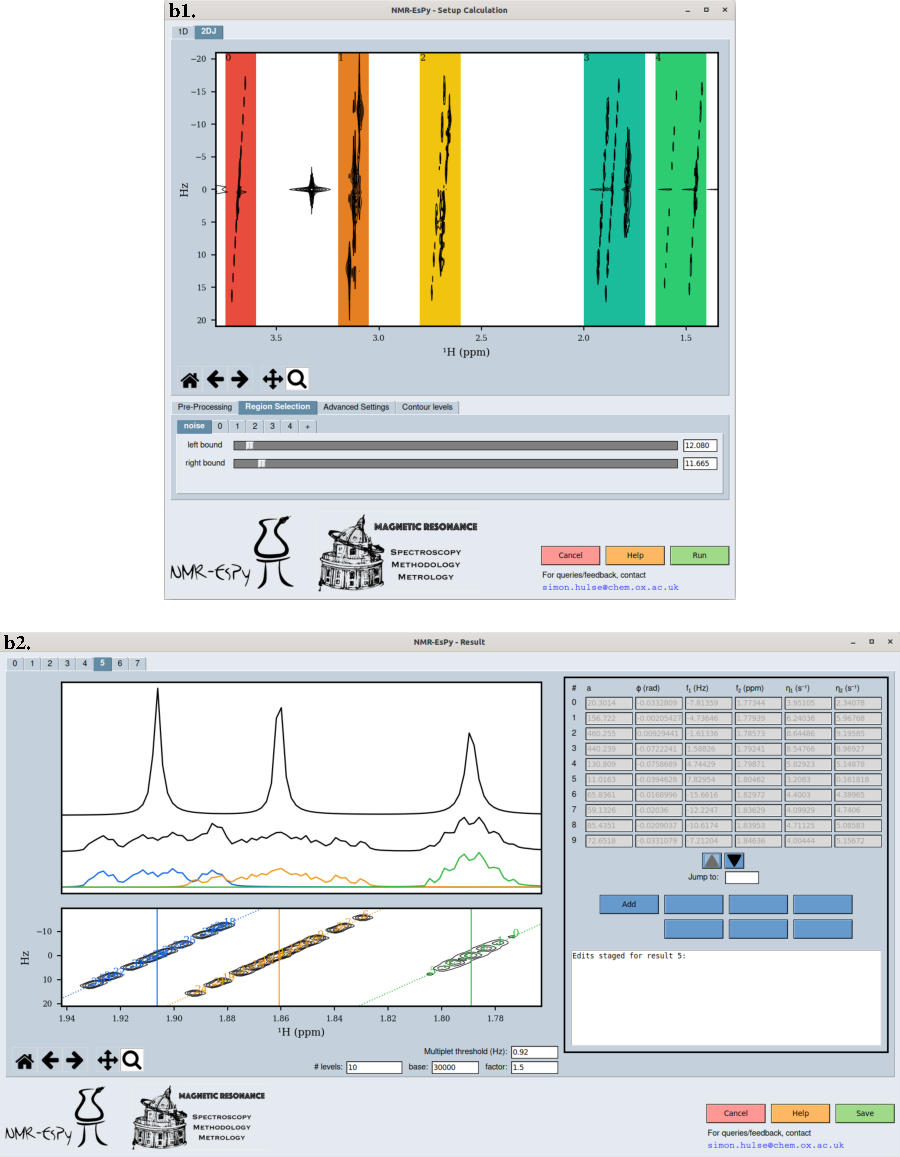
\includegraphics{gui/gui_2dj.pdf}
    \caption*{Continuation of \textbf{\textsc{\cref{fig:gui}}}.}
\end{figure}
Along with the \ac{EsPy} \ac{API}, an accompanying \ac{GUI} based on the
\textsc{Tkinter} toolkit ships with the
package. This can be accessed either via the command line, or within
\textsc{Bruker}'s \textsc{TopSpin} software to provide a more seamless workflow
in analysing \ac{NMR} data acquired on \textsc{Bruker} spectrometers.
At the time of writing, the \ac{GUI} only supports conventional \ac{1D}
and \ac{2DJ} datasets. Screenshots of the \acp{GUI} for both data types are
provided in \cref{fig:gui}.
The \ac{GUI} comprises two primary windows; the first enables the estimation
routine to be set up (panels a1 \& b1), while the second is for inspecting the
result (panels a2 \& b2). For the set-up window, the following actions are
carried out by the user:
\begin{itemize}
    \item The \emph{Pre-Processing} tab enables phase correction,
        application of exponential line-broadening\footnote{
            Exponential line-broadening is the only type of apodisation which
            is supported in \ac{EsPy}; use of any other window function
            would render the model used to fit the data incompatible.
            Line-broadening should only be applied in
            situations where the \ac{FID} is truncated, such that sinc wiggles
            are visible in the spectrum, as these will have an unwanted
            influence on filtered sub-\acp{FID} generated.
        }, and baseline correction. If the imported data has already been
        processed by some other software such as \textsc{TopSpin}\footnote{
            For \ac{1D} datasets, it is possible to import raw \ac{FID} data
            (\texttt{fid}) or processed spectral data (\texttt{1r}). If
            pre-processed data is imported, \ac{EsPy} performs \ac{IFT} and
            truncates the conjugate-symmetric signal generated in half to
            recover the \ac{FID}. For \ac{2DJ} data, it is necessary to import
            \ac{2DJ} data as a raw \ac{FID} (\texttt{ser}).
        }, this step can be skipped.
    \item Regions of interest and a region to determine the noise variance are
        specified with the \emph{Region Selection} tab. Panels a1 and b1 in
        \cref{fig:gui} provide illustrations of the appearance of the
        \ac{GUI} after a number of regions\,---\,each denoted by a coloured
        rectangle\,---\,have been defined by the user.
    \item \emph{Additional Setting} allows features related to the estimation
        routine to be customised, including whether to approximate the Hessian
        matrix or compute its exact form; whether to predict the model order
        using the \ac{MDL} or to manually specify a value; and setting a
        threshold for the maximum number of iterations allowed.
\end{itemize}

The result window effectively features a figure depicting the outcome of the
estimation routine, with a table of all the estimated parameters. For any
features in the result which the user deems to be erroneous, there is scope for
some basic edits to be made to be. Oscillators can be \emph{added} to the
result if a particular signal has been missed by the routine; they can be
\emph{removed} if they are deemed spurious; multiple oscillators can be
\emph{merged} if a particular signal is deemed to be over-fit; and a single
oscillator can be \emph{split} if more than one signal is deemed to be
under-fit. If any edits are requested by the user, the updated parameter set is
subjected to \ac{NLP} in order to reduce the bias in the result, and ensure
good agreement between the model and data is maintained. The ability to edit
the result can lead to better outcomes, since the user is able to guide the
optimiser using their expertise. The final stage in using the \ac{GUI}
involves specifying the formats to output the result to. Both figures and
parameter tables summarising the result can be exported to various formats. As
well as this, the estimator object which conducted everything under the hood
can be saved to a byte stream for future inspection.

\section{Summary}
In this chapter, an overview of the software associated with this project, a
\textsc{Python} package call \ac{EsPy}, has been provided.
There are more resources available for additional information on \ac{EsPy}. A rigorous
description of the usage of \ac{EsPy}, including details on installation, and a
reference for the \ac{API} are given in the documentation for \ac{EsPy}, found
at \url{https://foroozandehgroup.github.io/NMR-EsPy/}.
One chapter of the documentation, which provides tutorials to help users gain
familiarity with the \ac{API}, is included in this work (see \cref{chap:inserts}.1).
\ac{EsPy} is open source, under the \textsc{MIT} license, with the source code
hosted on the Foroozandeh group's \textsc{GitHub} page at
\url{https://github.com/foroozandehgroup/NMR-EsPy}.


\chapter{Conclusions and Future Work}
\label{chap:conclusions}

\section{Conclusions}
This work has focussed on the use of parametric estimation as a means of
extracting quantitative information from \ac{NMR} \acp{FID}. The initial
motivation for it arose due to an interest in developing a technique
which could analyse \ac{2DJ} datasets, facilitating the generation of broadband
homodecoupled \ac{NMR} spectra with desirable characteristics.
To achieve this, the \ac{MMEMPM}, a \ac{2D} extension of the original \ac{MPM},
was proposed as a suitable estimation routine for considering \ac{2DJ} datasets
in a holistic fashion.
However, initial evaluations of results generated by the \ac{MPM} on
\ac{1D} \acp{FID} indicated that a particular flaw frequently arose: the phases
of oscillators in the estimated model were commonly inconsistent with
expectations based on the data structure.
For this reason, a routine was developed which used the result of the
\ac{MPM} as the initial guess of \iac{NLP} algorithm; the \ac{NLP} algorithm
included the variance of oscillator phases in its fidelity to overcome the
undesirable phase behaviour.
Through a number of examples, it has been shown that improved parameter
estimates can be obtained relative to the \ac{MPM} isolation.
It is expected that improved results could be obtained when iterative routines
which incorporate large amounts of user-provided information are used, such as
\ac{AMARES}. The uptake of these methods is minimal in \ac{NMR} however, due to
the impracticality in supplying the information required. The routine described
in this thesis aims to be a compromise between the \ac{MPM}, requiring no user
information, and those like \ac{AMARES}.

To alleviate the high computational burden of the proposed method\,---\,the
most noteworthy aspects being determining the \ac{SVD} of large matrices and
computing Hessian of the \ac{NLP} fidelity\,---\,a frequency-filtration
technique has been incorporated. This produces sub-\acp{FID} with reduced
numbers of both constituent signals and datapoints, breaking down the
estimation problem into a number of smaller-scale ones.
Drastic reductions in both \ac{CPU} work and \ac{RAM} usage are possible by
doing this.
Furthermore, data filtration enables the user to neglect spectral regions
that are not of interest/too crowded to realistically yield meaningful
information from. A specification of the regions to estimate is the primary
piece of information that must be supplied manually by the user.
Work which hasn't been discussed in this thesis was carried out in an attempt to
automate this, though with minimal success\footnote{
    The approach to automate the determination of spectral regions was based on
    the concept of classifying points which belong to the spectral
    baselines\cite{Dietrich1991}; any section of the spectrum which comprised a
    sufficiently large number of consecutive points which were not classified
    as baseline was deemed to be a region of interest. Alas, this approach
    proved to be rather temperamental, with considerable tweaking of
    hyperparameters necessary to yield reasonable results. For this reason, the
    concept was discarded.
}.

Impressive parametrisations of hypercomplex \ac{2DJ} \acp{FID} were achieved using
the estimation routine, leading to \ac{CUPID}, which is able generate pure
shift spectra without the loss of signal associated with experimental
``chunking'' methods, and featuring peaks with sharp absorption Lorentzian
lineshapes.
Furthermore, \ac{CUPID} is able to provide additional insights, such as
harnessing the information from \ac{2DJ} estimation to decompose \ac{1D}
spectra into their constituent multiplet structures. Acquiring the information
that \ac{CUPID} can generate with a simple \ac{2DJ} dataset usually requires
bespoke \ac{3D} pulse sequences with a very large associated run-times.

Beyond to the original goal of \ac{2DJ} estimation, two other applications
have been developed and presented here. The first is an alternative means for
determining valuable information about molecular species ($T_1$ and  $T_2$
times of spins, and diffusion coefficients) via datasets which comprise a series
of \acp{FID} whose amplitudes vary. Whereas typical univariate
approaches to analysing these datasets involve fitting single datapoints in
frequency space, the method showcased instead aims to gleam the
information for each signal explicitly, to overcome the aggregating effect
frequently encountered due to signal overlap. While the method works admirably,
it couldn't be shown to perform noticeably better than other techniques; in
cases where there is severe signal crowding, the difficulty/impossibility of
resolving each component leads to similar issues involving signal aggregation.

A second application featuring \ac{1D} estimation involves generating broadband
\ac{NMR} spectra from an experiment involving excitation by a single chirp
pulse. With appropriate processing, involving estimating each signal using the
\ac{MPM}, and appropriately back-propagating it based on its frequency, phase
spectra with flat baselines are achievable.
This work is fairly nascent, and while the initial results presented here show
promise, there is yet to be applied to datasets of greater interest. If
further results indicate the method is effective, this could lead to improved
sensitivity for ultra-broadband spectra, when compared with current
state-of-the-art methods like \ac{CHORUS}.

The software package \ac{EsPy} has been developed to facilitate use of the methods
described in this thesis. The package's \ac{API} follows a straightforward
object-oriented paradigm, which should make it easily accessible to all
members of the \ac{NMR} community that have experience of scientific
computing with \Python\!. Furthermore, the availability of an accompanying \ac{GUI}
widens to accessibility of the package further, meaning \ac{EsPy} can be used
without writing a single line of code. The package has been heavily documented
too; this is a crucial element for any user-facing software which is often
lacking, especially in academic contexts.

%%% Final bit
It has hopefully been shown that attempting to solve the inverse problem of
\ac{NMR} data estimation is a valuable pursuit; it provides richer information
that that which is typically available with the conventional \ac{FT} method,
and it opens up many fruitful applications which can enhance the value that
\ac{NMR} can offer to practitioners in many scientific disciplines.


\section{Future Work}
\label{sec:future-work}
Any future work related to this project would be centered around extending and
improving the \ac{EsPy} package. Some possible pursuits include the following:

\paragraph{Improving performance}
Improvements in the speed of the estimation
could be realised if the most computationally demanding parts of it were
written in a low-level compiled language like C++ or \textsc{Rust}. This may not
be the case for the \ac{MPM} and \ac{MMEMPM}; the majority of time running
these routines involves \ac{SVD}, with \textsc{NumPy}'s implementation calling
well-optimised routines from the \textsc{LAPACK} and \textsc{ARPACK} software
packages. However, in its current state, the \ac{NLP} routine could well be
sped up considerably if the current \Python implementation were ported to one
of the aforementioned languages.

\paragraph{A more general platform}
Thinking further afield from the specific estimation routine considered in this
work, the \ac{EsPy} package provides a large number of useful features which
would be applicable to the estimation using any conceived method. The includes
functionality to import data, pre-process data, and inspect the result of an
estimation routine through parameter tables and figures.
Incorporating other estimation routines into the software would therefore be
rather straightforward, such that \ac{EsPy} could become a general-purpose
platform for comparing different methods.

\paragraph{\ac{2D} and \ac{3D} datasets}
Another potential future venture would be to extend to routine for the
consideration of other \ac{2D} datasets, such as those that comprise
amplitude- or phase-modulated pairings, as well as \ac{3D} datasets,
including those acquired from ``triple-resonance'' experiments which are
popular in the biological \ac{NMR} community\cite[Section 7.4]{Cavanagh2007}.
As shown in
\cref{chap:cupid}, the method is capable of performing well on hypercomplex
\ac{2D} datasets. In order to achieve \ac{3D} estimation, it would be necessary to
make use of a \ac{3D} equivalent of the \ac{MMEMPM}. Such a technique exists,
and is used principally for sensing applications, in which the direction (i.e.
azimuth and elevation angles) as well as the frequency of waves arriving at an
antenna are sought\cite{Yilmazer2006}. However, there is a key issue with
multidimensional \ac{NMR} signals which would likely hamper the method outlined
in this thesis from being effective. \ac{2DJ} datasets are rather anomalous in
that they have very densely populated indirect dimensions. For this reason, it
is not necessary to be concerned about filtering the data in the indirect
dimension. However, for most \ac{2D} datasets, it would be desirable to filter
the data in both dimensions, as both will generally be sparsely populated.
While the filtering procedure presented works well on direct-dimension
\acp{FID}, which have usually decayed to noise at the end
of acquisition, indirect-dimension \acp{FID} are often truncated. The \ac{FT}
of such signals without any treatment would produce spectra with considerable
truncation artefacts; filtering such spectra would incorporate undesirable
artefacts into a filtered sub-\ac{FID}, rendering it worthless.
Compensating for the truncation could be achieved, by applying exponential
apodisation prior to \ac{FT}. However, this would then lead to spectra with
broader lineshapes, such that wider spectral regions would need to be selected,
and the resolution of the data would be decreased.
Dealing with
truncated signals could possibly be handled in one of two ways, beyond running
the experiment to acquire the data with a huge number of increments. One
option would be to propagate the \ac{FID} further in time using \ac{LP}.
Another would be to apply conventional apodisation, such as a sine-bell
function to the \ac{FID}, producing a \ac{FID} without truncation artefacts and
acceptable resolution. However, applying a non-exponential weighting to the
dataset however render the data incompatible with the estimation routine in its
current form, such that a modified routine with a suitable model would need to
be implemented. On to of issues with data applicability, for \ac{3D}
estimation the computational burden required would also likely be too high for
the routine to be practicable beyond the simplest datasets with few points and
minimal numbers of signals.

\paragraph{Incorporating constraints into the \ac{NLP} routine}
The estimation routine in its current form is designed to require as little
user input as possible while producing faithful parameter estimates. However,
in particularly challenging circumstances, most notably when
there is extreme signal overlap, the inclusion of oscillator phase variance
alone can be insufficient to produce estimates which closely agree with the
experiment. When this is the case, it would be useful to enable users to
specify additional knowledge, incorporated into the routine as additional
regularising terms, \emph{after} the initial estimation has been performed.
This concept, while similar to \ac{VARPRO} and \ac{AMARES}, differs in that
these require very large quantities or prior knowledge \emph{before}
estimation. A lot of the heavy lifting towards an accurate parameter estimate
could be achieved using phase variance-regularised \ac{NLP}, with the user
indicating erroneous features subsequently.

Take the cyclosporin A result (\cref{fig:cyclosporin}) as an example. As
discussed already, due to severe signal overlap, the assigned oscillators
related to spin (E), while at the correct frequencies, do not have appropriate
amplitudes for a dq multiplet structure. As such, re-running \ac{NLP}, with a
new fidelity of
\[
    \FphithY + \Var(
        a_{\text{E}1},
        \tfrac{1}{3} a_{\text{E}2},
        a_{\text{E}3},
        \tfrac{1}{3} a_{\text{E}4},
        \tfrac{1}{3} a_{\text{E}5},
        a_{\text{E}6},
        \tfrac{1}{3} a_{\text{E}7},
        a_{\text{E}8}
    )
\]
would likely lead to an improved result.
$\lbrace \text{E}1, \cdots, \text{E}8 \rbrace \subset \lbrace 1, \cdots, M \rbrace$ are the
indices of the oscillators corresponding to spin (E), i.e. the green
oscillators in the figure.

\printbibliography
\appendix
\renewcommand{\thealgorithm}{A\arabic{algorithm}}
\renewcommand{\thefigure}{A\arabic{figure}}
\renewcommand{\thetable}{A\arabic{table}}
\setcounter{algorithm}{0}
\setcounter{figure}{0}
\setcounter{table}{0}
\chapter{Additional Theory}

\section{Mathematical definitions}

Descriptions of linear algebra and statics concepts that are referred to in
this thesis are provided here. More detail can be found in numerous relevant
texts\cite{Strang2018,Pawitan2001}.

\subsection{Linear algebra}
\label{subsec:linear-algebra}

\note{TODO: rank, range}

\subsubsection{\Acl{SVD}}
\ac{SVD} is a generalisation of eigendecomposition for a matrix of any shape.
Given a matrix $\symbf{A} \in \mathbb{C}^{m \times n}$, the \ac{SVD} is a
factorisation given by
\begin{equation}
    \symbf{A} = \symbf{U} \symbf{\Sigma} \symbf{V}^{\dagger}.
\end{equation}
The matrices that make up the decomposition are as follows
\begin{itemize}[label={}]
    \item $\symbf{\Sigma} \in \mathbb{C}^{m \times n}$ is a rectangular
        diagonal matrix with diagonal elements comprising the \emph{singular
        values} in descending order of magnitude. The singular values are the
        square roots of the non-zero eigenvalues of both
        $\symbf{A}^{\dagger}\symbf{A}$ and
        $\symbf{A}\symbf{A}^{\dagger}$.
    \item $\symbf{U} \in \mathbb{C}^{m \times m}$ is a unitary matrix whose columns
        comprise the \emph{left singular vectors}. The left singular vectors
        are the eigenvectors of the matrix $\symbf{A}\symbf{A}^{\dagger}$.
    \item $\symbf{V} \in \mathbb{C}^{n \times n}$ is a unitary matrix whose columns
        comprise the \emph{right singular vectors}. The right singular vectors
        are the eigenvectors of the matrix $\symbf{A}^{\dagger}\symbf{A}$.
\end{itemize}
One fundamental property of the \ac{SVD} is that the number of non-zero
singular values is equivalent to the rank of the matrix. As the \ac{EYM}
theorem highlights, the \ac{SVD} is valuable in constructing low-rank
approximations of matrices, with applications in various fields such as signal
processing, (see Section \ref{subsec:mpm}) and data compression.

\subsubsection{Special matrices}
A \emph{Hankel matrix} is a matrix in which each ascending diagonal from left to right
possesses identical elements. While Hankel matrices are often defined to be square, in
this work such a restriction is not applied. Given a matrix $\symbf{X} \in
\mathbb{F}^{M \times N}$, the matrix is Hankel if
\begin{equation}
    x_{m,n} = x_{m+1,n-1}
\end{equation}
$\forall m \in \lbrace 1, \cdots, M-1 \rbrace
\ \forall n \in \lbrace 2, \cdots, N \rbrace$.
Similarly, a \emph{Toeplitz matrix} is a matrix in which every descending
diagonal from left to right possesses identical elements, i.e.
\begin{equation}
    x_{m,n} = x_{m+1,n+1}
\end{equation}
$\forall m \in \lbrace 1, \cdots, M-1 \rbrace\ \forall n
\in \lbrace 1, \cdots N-1, \rbrace$.

\subsection{Statistics and probability}

\note{TODO: Likelihood function, MLE}

\subsubsection{\Acl{pdf}}
The \ac{pdf} $p(x) : \mathbb{R} \rightarrow \mathbb{R}$ is a function over a
continuous sample space which provides relative likelihoods between potential
values of $x$.  The probability that a random sample obeying a known
distribution lies withing the range $[x_a, x_b]$ is given by the integral
\begin{equation}
    P(x_a \leq x \leq x_b) = \int_{x_a}^{x_b} p(x) \mathrm{d}x.
\end{equation}
The integral of $p(x)$ over the entire sample space is defined to be
unity. Also, the \ac{pdf} of a specific value is always $0$, since the width of
the region of integration is $0$.

\subsubsection{Likelihood function}

\section{Multidimensional \aclp{VE}}
\label{sec:multidim-ve}
The \ac{VE} concept (Section \ref{subsec:ve}) can be generalised to any number
of dimensions, assuming that a pair of amplitude-modulated signals exist for
each indirect-dimension. Thus a set of $2^{D-1}$ signals is required for a
$D$-dimensional \ac{FID}.
For the \ac{2D} case, this corresponds to the pair of signals $\lbrace
\bY^{\cos}, \bY^{\sin} \rbrace$, given by \eqref{eq:general-fid} with $D=2$ and
$\zeta = \lbrace \cos(\cdot), \sin(\cdot) \rbrace$, taking the forms (with
noise neglected)
\begin{subequations}
    \begin{gather}
        y^{\cos}_{\none,\ntwo} =
            \xi^{\vphantom{(1)}}_{\none,\ntwo}
            c^{(1)}_{\none,\ntwo}
            \left(c^{(2)}_{\none,\ntwo} + \iu s^{(2)}_{\none,\ntwo}\right),\\
        y^{\sin}_{\none,\ntwo} =
            \xi^{\vphantom{(1)}}_{\none,\ntwo}
            s^{(1)}_{\none,\ntwo}
            \left(c^{(2)}_{\none,\ntwo} + \iu s^{(2)}_{\none,\ntwo}\right),\\
        \xi^{\vphantom{(1)}}_{\none,\ntwo} =
            \sum_m a_m \exp\left(-\etaonem \none \Dtone -\etatwom \ntwo \Dttwo\right),\\
        (c/s)^{(1/2)}_{\none,\ntwo} =
            \sum_m \cos / \sin \left(2 \pi f^{(1/2)} n^{(1/2)} \Updelta^{(1/2)}\right).
    \end{gather}
\end{subequations}
Four matrices $\symbf{\psi}_{\pm\pm}$ are then constructed of the form
\begin{equation}
    \begin{gathered}
        \psi_{\pm\pm, \none, \ntwo} =
            \xi_{\none,\ntwo}^{\vphantom{(1)}}
            \left(c^{(1)}_{\none,\ntwo} \pm^{(1)} \iu s^{(1)}_{\none,\ntwo}\right)
            \left(c^{(2)}_{\none,\ntwo} \pm^{(2)} \iu s^{(2)}_{\none,\ntwo}\right)\\
         \equiv
             \Re\left( y^{\cos}_{\none,\ntwo} \right)
             \pm^{(1)} \pm^{(2)} -
             \Im\left( y^{\sin}_{\none,\ntwo} \right)
             + \iu \left(
             \pm^{(1)}
             \Re\left( y^{\sin}_{\none,\ntwo} \right)
             \pm^{(2)}
             \Im\left( y^{\cos}_{\none,\ntwo} \right)
             \right),
    \end{gathered}
\end{equation}
from which the matrices $\symbf{T}_{1 \rightarrow 4} \in \mathbb{C}^{2 \None
\times 2 \Ntwo}$ are generated:
\begin{subequations}
    \begin{gather}
        \symbf{T}_1 =
        \begin{bmatrix}
            \symbf{\Psi}_{++} & \symbf{0} \\
            \symbf{0} & \symbf{0}
        \end{bmatrix}, \\
        \symbf{T}_2 =
        \begin{bmatrix}
            \symbf{0} & \symbf{0} \\
            \symbf{\Psi}_{-+}^{\leftrightsquigarrow (1)} & \symbf{0}
        \end{bmatrix}^{\circlearrowright (1)}, \\
        \symbf{T}_3 =
        \begin{bmatrix}
            \symbf{0} & \symbf{\Psi}_{+-}^{\leftrightsquigarrow (2)} \\
            \symbf{0} & \symbf{0}
        \end{bmatrix}^{\circlearrowright (2)}, \\
        \symbf{T}_4 =
        \begin{bmatrix}
            \symbf{0} & \symbf{0} \\
            \symbf{0} & \symbf{\Psi}_{--}^{\leftrightsquigarrow (1,2)}
        \end{bmatrix}^{\circlearrowright (1,2)}.
    \end{gather}
\end{subequations}
The virtual echo is then given by $\symbf{Y}_{\text{ve}} = \sum_{i=1}^4
\symbf{T}_i$, with the first row and column divided by two. For a full outline
of the 2D filtering procedure, see Algorithm \ref{alg:filter-2d}.

It is possible to construct a virtual echo using an appropriate set of
phase-modulated signals too, which for the \ac{2D} case would be $\lbrace
\symbf{Y}^{\text{pos}}, \symbf{Y}^{\text{neg}}\rbrace$, given by
\eqref{eq:general-fid} with $D=2$ and  $\zeta = \lbrace \exp(\iu \cdot),
\exp(-\iu\cdot)\rbrace$. These can be used to generate an amplitude modulated pair via
\begin{subequations}
    \begin{gather}
        \symbf{Y}^{\text{cos}} = \frac{\symbf{Y}^{\text{pos}} + \symbf{Y}^{\text{neg}}}{2},\\
        \symbf{Y}^{\text{sin}} = \frac{\symbf{Y}^{\text{pos}} - \symbf{Y}^{\text{neg}}}{2\iu}.
    \end{gather}
\end{subequations}



\section{Additional algorithms}
\null\vfill
\begin{algorithm}[h!]
    \caption{The \acs{MMEMPM}.}
    \label{alg:mmempm}
    \begin{algorithmic}[1]
        \Procedure {MMEMPM}{$\symbf{Y} \in \mathbb{C}^{\None \times \Ntwo}, M \in \mathbb{N}$}
        \State $\Lone, \Ltwo \gets \left\lfloor \nicefrac{\None}{2} \right\rfloor, \left\lfloor \nicefrac{\Ntwo}{2} \right\rfloor$;
        \For{$\none \gets \lbrace 0, \cdots, \None - 1 \rbrace$}
            \State  $\symbf{H}_{\symbf{Y},\none} \gets
                \def\arraystretch{1.4}
            \begin{bmatrix}
                \symbf{Y}\left[\none, 0\right] &
                \symbf{Y}\left[\none, 1\right] &
                \cdots &
                \symbf{Y}\left[\none, \Ntwo-L^{(2)}\right]\\
                \symbf{Y}\left[\none, 1\right] &
                \symbf{Y}\left[\none, 2\right] &
                \cdots &
                \symbf{Y}\left[\none, \Ntwo-L^{(2)}+1\right]\\
                \vdots & \vdots & \ddots & \vdots\\
                \symbf{Y}\left[\none, L^{(2)} - 1\right] &
                \symbf{Y}\left[\none, L^{(2)}\right] &
                \cdots &
                \symbf{Y}\left[\none, \Ntwo-1\right]\\
            \end{bmatrix}
        $
        \EndFor;
        \State $\symbf{E}_{\symbf{Y}} \gets
        \begin{bmatrix}
            \symbf{H}_{\symbf{Y},0} & \symbf{H}_{\symbf{Y},1} & \cdots & \symbf{H}_{\symbf{Y},\None - L^{(1)}}\\
            \symbf{H}_{\symbf{Y},1} & \symbf{H}_{\symbf{Y},2} & \cdots & \symbf{H}_{\symbf{Y},\None - L^{(1)} + 1}\\
            \vdots & \vdots & \ddots & \vdots\\
            \symbf{H}_{\symbf{Y},L^{(1)} - 1} & \symbf{H}_{\symbf{Y},L^{(1)}} & \cdots & \symbf{H}_{\symbf{Y},\None - 1}
        \end{bmatrix}
        $;
        \State $\symbf{U}_M^{\vphantom{\dagger}},
            \symbf{\Sigma}_M^{\vphantom{\dagger}},
            \symbf{V}_M^{\dagger} \gets
            \textsc{TruncatedSVD}\left(\EY, M\right)$;
        \State $\symbf{P} \gets \symbf{0} \in \mathbb{C}^{\Lone \Ltwo \times \Lone \Ltwo}$;
        \State $r \gets 0$
        \For{$i = 0, \cdots, \Ltwo - 1$}
            \For{$j = 0, \cdots, \Lone - 1$}
                \State $c \gets i + j \Ltwo$;
                \State $\symbf{P}\left[r, c\right] \gets 1$;
                \State $r = r + 1$;
            \EndFor
        \EndFor
        \State $\symbf{U}_{M1}, \symbf{U}_{M2} \gets \symbf{U}_M\left[ : L^{(1)}(L^{(2)}-1)\right], \symbf{U}_M\left[L^{(2)}:\right]$;
        \Comment{Last/First $L^{(2)}$ rows deleted}
        \State $\symbf{z}^{(1)}, \symbf{W}^{(1)} \gets \textsc{Eigendecomposition}\left( \symbf{U}_{M1}^+ \symbf{U}_{M2}^{\vphantom{+}} \right)$;
        \State $
            \symbf{f}^{(1)},
            \symbf{\eta}^{(1)} \gets
            \left(
                \nicefrac{f_{\text{sw}}^{(1)}}{2 \pi}
            \right)
            \Im \left( \ln \symbf{z}^{(1)} \right) + \foffone,
            -\fswone \Re \left( \ln \symbf{z}^{(1)} \right)
        $;
        \State $\symbf{U}_{M\text{P}} \gets \symbf{P} \symbf{U}_M$;
        \State $
            \symbf{U}_{M\text{P}1},
            \symbf{U}_{M \text{P} 2} \gets
            \symbf{U}_{M \text{P}}\left[ : (L^{(1)}-1)L^{(2)}\right],
            \symbf{U}_{M \text{P}}\left[L^{(1)}:\right]
        $;
        \Comment{Last/First $L^{(1)}$ rows deleted}
        \State $
            \symbf{z}^{(2)} \gets \operatorname{diag} \left(
                \left[\symbf{W}^{(1)}\right]^{-1}
                \symbf{U}_{M\text{P}1}^{+}
                \symbf{U}_{M\text{P}2}^{\vphantom{+}}
                \symbf{W}^{(1)}
            \right)$;
        \State $
            \bdftwo,
            \bdetatwo \gets
            \left(
                \nicefrac{\fswtwo}{2 \pi}
            \right)
            \Im \left( \ln \symbf{z}^{(2)} \right) + \fofftwo,
            -\fswtwo \Re \left( \ln \symbf{z}^{(2)} \right)
        $;
        \State $
        \symbf{Z}^{(2)}_{\text{L}} =
        \begin{bmatrix}
            \symbf{1} &
            \bdztwo &
            {\bdztwo}^2 &
            \cdots &
            {\bdztwo}^{\Ltwo-1}
        \end{bmatrix}\T
        $;
        \State $
            \symbf{Z}^{(2)}_{\text{R}} \gets
            \begin{bmatrix}
                \symbf{1} & \bdztwo & {\bdztwo}^2 & \cdots & {\bdztwo}^{\Ntwo - \Ltwo}
            \end{bmatrix}
        $;
        \State $\symbf{Z}^{(1)}_{\text{D}} \gets \diag\left(\bdzone\right)$;
       \State $
            \symbf{E}_{\text{L}} \gets
            \begin{bmatrix}
                \symbf{Z}^{(2)}_{\text{L}} \\
                \symbf{Z}^{(2)}_{\text{L}} \symbf{Z}^{(1)}_{\text{D}} \\
                \vdots\\
                \symbf{Z}^{(2)}_{\text{L}} \left[\symbf{Z}^{(1)}_{\text{D}}\right]^{\Lone - 1}
            \end{bmatrix}
        $;
        \State $
            \symbf{E}_{\text{R}} \gets
            \begin{bmatrix}
                \symbf{Z}^{(2)}_{\text{R}} &
                \symbf{Z}^{(1)}_{\text{D}} \symbf{Z}^{(2)}_{\text{R}} &
                \cdots &
                \left[\symbf{Z}^{(1)}_{\text{D}}\right]^{\None - \Lone} \symbf{Z}^{(2)}_{\text{R}}
            \end{bmatrix}
        $;
        \State $
           \bdalpha \gets \diag
           \left(
               \symbf{E}_{\text{L}}^+
               \symbf{E}_{\symbf{Y}}^{\vphantom{+}}
               \symbf{E}_{\text{R}}^+
           \right)
           $;
        \State $
            \bda, \bdphi \gets
            \left\lvert \bdalpha \right\rvert,
            \arctan \left( \frac{\Im\left(\bdalpha\right)}{\Re\left(\bdalpha\right)} \right)
        $;
        \State $\symbf{\theta}^{(0)} \gets
        \begin{bmatrix}
            \bda\T &
            \bdphi\T &
            \left[\symbf{f}^{(1)}\right]\T &
            \left[\symbf{f}^{(2)}\right]\T &
            \left[\symbf{\eta}^{(1)}\right]\T &
            \left[\symbf{\eta}^{(2)}\right]\T
        \end{bmatrix}
        ^{\mathrm{T}}$;
        \State \textbf{return} $\symbf{\theta}^{(0)}$
    \EndProcedure
    \end{algorithmic}
\end{algorithm}
\vfill\null



\begin{algorithm}
    \caption[
        Steihaug-Toint method for determining an update for nonlinear
        programming.
    ]{
        Steihaug-Toint method for determining an update for nonlinear
        programming. This is equivalent to Algorithm 7.2 in \cite{Nocedal2006}.
    }
    \label{alg:steihaug-toint}
    \begin{algorithmic}[1]
        \Procedure{SteihaugToint}{
            $\bY \in \mathbb{C}^{\None \times \cdots \times \ND},
            \bthk \in \mathbb{R}^{2(1 + D)M},
            \trustradius{k} \in \mathbb{R}_{>0}
            $
        }
            \State $\symbf{g} \gets \nabla \FphithkY$;
            \Comment{Grad vector: \eqref{eq:grad}}
            \State $\symbf{H} \gets \nabla^2 \FphithkY$;
            \Comment{Hessian matrix, either exact: \eqref{eq:hess} or approximate: \eqref{eq:hess-approx}}
            \State $\epsilon^{(k)} \gets \min\left(
                    \nicefrac{1}{2},
                    \sqrt{\left\lVert \symbf{g} \right\rVert}
                \right)
                \left\lVert \symbf{g} \right\rVert
                $;
            \State $\symbf{z}^{(0)} \gets \symbf{0} \in \mathbb{R}^{6M}$;
            \State $\symbf{r}^{(0)} \gets \symbf{g}$;
            \State $\symbf{d}^{(0)} \gets -\symbf{r}^{(0)}$;
            \If {$\left \lVert \symbf{r}^{(0)} \right \rVert < \epsilon^{(k)}$}
                \State \textbf{return} $\symbf{z}^{(0)}$;
            \EndIf
            \For {$j = \lbrace 0, 1, \cdots \rbrace$}
                \If {
                    ${\symbf{d}^{(j)}}^{\mathrm{T}}
                    \symbf{H}
                    \symbf{d}^{(j)}
                    \leq 0$
                }
                \State Find $\tau$ such that $\symbf{p}^{(k)} = \symbf{z}^{(j)} + \tau \symbf{d}^{(j)}$
                    minimises $\FphiQthkpk$, subject to
                    $\left \lVert \symbf{p}^{(k)} \right \rVert = \trustradius{k}$;
                    \State \textbf{return} $\symbf{p}^{(k)}$;
                \EndIf
                \State $\alpha^{(j)} \gets \dfrac
                    {{\symbf{r}^{(j)}}^{\mathrm{T}} \symbf{r}^{(j)}}
                    {
                        {\symbf{d}^{(j)}}^{\mathrm{T}}
                        \symbf{H}
                        \symbf{d}^{(j)}
                    }$;
                \State $\symbf{z}^{(j+1)} \gets \symbf{z}^{(j)} + \alpha^{(j)} \symbf{d}^{(j)}$;
                \If {$\left \lVert \symbf{z}^{(j+1)} \right \rVert < \epsilon^{(k)}$}
                    \State Find $\tau \in \mathbb{R}_{>0}$ such that
                        $\symbf{p}^{(k)} = \symbf{z}^{(j)} + \tau \symbf{d}^{(j)}$
                        satisfies
                        $\left \lVert \symbf{p}^{(k)} \right \rVert = \trustradius{k}$;
                    \State \textbf{return} $\symbf{p}^{(k)}$;
                \EndIf
                \State $\symbf{r}^{(j+1)} \gets
                    \symbf{r}^{(j)} +
                    \alpha^{(j)}
                    \symbf{H}
                    \symbf{d}^{(j)}$;
                    \If{$\left\lVert \symbf{r}^{(j+1)} \right \rVert < \epsilon^{(k)}$}
                    \State \textbf{return} $\symbf{z}^{(j+1)}$;
                \EndIf
                \State $\beta^{(j+1)} \gets
                    \dfrac{{\symbf{r}^{(j+1)}}^{\mathrm{T}} \symbf{r}^{(j+1)}}{{\symbf{r}^{(j)}}^{\mathrm{T}} \symbf{r}^{(j)}}$;
                \State $\symbf{d}^{(j+1)} \gets -\symbf{r}^{(j+1)} + \beta^{(j+1)} \symbf{d}^{(j)}$;
            \EndFor
        \EndProcedure
    \end{algorithmic}
\end{algorithm}



\begin{algorithm}[h!]
    \begin{algorithmic}[1]
        \caption[
            Filtering procedure for 1D data.
        ]
        {
            Filtering procedure for 1D data.
            $\symbf{r}_{\text{interest}}$ is a vector of length 2 containing
            the indices of the left and right bounds of the region of interest.
            These would typically be provided in units of \unit{\hertz} or
            \unit{\partspermillion} by a user. Conversion to array indices can
            be carried out using \eqref{eq:fidx}.
            $\symbf{r}_{\text{noise}}$ contains the left and right bounds of
            the region used to estimate the noise variance.
            \textsc{RandomSample} indicates taking a random sample from the
            given distribution.
        }
        \label{alg:filter-1d}
        \Procedure{Filter$1$D}{
            $\by \in \mathbb{C}^{\None},
            \symbf{r}_{\text{interest}} \in \mathbb{N}_0^2,
            \symbf{r}_{\text{noise}} \in \mathbb{N}_0^2
            $}
            \State $\by_{\text{ve}} \gets \textsc{VirtualEcho$1$D}\left(\by\right)$;
            \State $\symbf{s}_{\text{ve}} \gets \FT\left(\by_{\text{ve}}\right)$;
            \State $l^{(1)}_{\text{idx}}, r^{(1)}_{\text{idx}} \gets \symbf{r}_{\text{interest}}[0], \symbf{r}_{\text{interest}}[1]$;
            \State $l^{(1)}_{\text{idx,noise}}, r^{(1)}_{\text{idx,noise}} \gets \symbf{r}_{\text{noise}}[0], \symbf{r}_{\text{noise}}[1]$;
            \State $c_{\text{idx}}^{(1)} \gets \nicefrac{\left(l_{\text{idx}}^{(1)} + r_{\text{idx}}^{(1)}\right)}{2}$;
            \State $b_{\text{idx}}^{(1)} \gets r_{\text{idx}}^{(1)} - l_{\text{idx}}^{(1)}$;
            \State $\symbf{g} \gets \textsc{SuperGaussian$1$D}\left(\None_{\vphantom{\text{idx}}}, c_{\text{idx}}^{(1)}, b_{\text{idx}}^{(1)}\right)$;
            \State $\symbf{s}_{\text{noise}} \gets \symbf{s}_{\text{ve}} \left[
                l^{(1)}_{\text{idx,noise}} : r^{(1)}_{\text{idx,noise}} + 1
            \right]
            $;
            \State $\sigma^2 \gets \Var\left(\symbf{s}_{\text{noise}}\right)$;
            \State $\symbf{w}_{\sigma^2} \gets \symbf{0} \in \mathbb{R}^{2\None}$;
            \For {$\none = 0, \cdots, \None - 1$}
                \State $\symbf{w}_{\sigma^2}\left[ \none \right] \gets \textsc{RandomSample}\left(\mathcal{N}\left(0, \sigma^2\right)\right)$;
            \EndFor
            \State $\widetilde{\symbf{s}}_{\text{ve}} \gets \symbf{s}_{\text{ve}} \odot \symbf{g} + \symbf{w}_{\sigma^2} \odot \left(\symbf{1} - \symbf{g}\right)$;
            \State $\widetilde{\symbf{y}}_{\text{ve}} \gets \IFT \left( \widetilde{\symbf{s}}_{\text{ve}} \right)$;
            \State $\widetilde{\symbf{y}} \gets \widetilde{\symbf{y}}_{\text{ve}}\left[ : \None \right]$;
            \State \textbf{return} $\widetilde{\symbf{y}}$;
        \EndProcedure
        \Statex
        \Procedure{VirtualEcho$1$D}{$\by \in \mathbb{C}^{\None}$}
            \State $\symbf{t}_1 \gets
            \begin{bmatrix}
                \by \\ \symbf{0} \in \mathbb{C}^{\None}
            \end{bmatrix}
            $;
            \State $\symbf{t}_2 \gets
            \begin{bmatrix}
            \symbf{0} \in \mathbb{C}^{\None} \\ {\by^*}^{\leftrightsquigarrow (1)}
            \end{bmatrix}^{\circlearrowright (1)}
            $;
            \State $\by_{\text{ve}} \gets \symbf{t}_1 + \symbf{t}_2$;
            \State $\by_{\text{ve}}[0] \gets \nicefrac{\by_{\text{ve}}[0]}{2}$;
            \State \textbf{return} $\by_{\text{ve}}$;
        \EndProcedure
        \Statex
        \Procedure{SuperGaussian$1$D}{$N \in \mathbb{N}, c_{\text{idx}} \in \mathbb{R}_{>0}, b_{\text{idx}} \in \mathbb{N}$}
            \State $\symbf{g} \gets \symbf{0} \in \mathbb{R}^{N}$;
            \For {$n = 0, \cdots, N - 1$}
                \State $\symbf{g}\left[ n \right] \gets \exp\left(
                    -2^{41} \left(
                        \frac{n - c_{\text{idx}}}{b_{\text{idx}}}
                    \right)^{40}
                    \right)
                $;
                \Comment{$p$ in \eqref{eq:super-Gaussian-onedim} has been set to 40.}
            \EndFor
            \State \textbf{return} $\symbf{g}$
        \EndProcedure
    \end{algorithmic}
\end{algorithm}

\begin{algorithm}[h!]
    \begin{algorithmic}[1]
        \caption{Filtering procedure for 2D data.}
        \label{alg:filter-2d}
        \Procedure{Filter$2$D}{$\bY_{\cos} \in \mathbb{C}^{\None \times \Ntwo}, \bY_{\sin} \in \mathbb{C}^{\None \times \Ntwo}, \symbf{R}_{\text{interest}} \in \mathbb{N}_0^{2 \times 2}, \symbf{R}_{\text{noise}} \in \mathbb{N}_0^{2 \times 2}$}
            \State $\bY_{\text{ve}} \gets \textsc{VirtualEcho$2$D}\left(\bY_{\cos}, \bY_{\sin}\right)$;
            \State $\symbf{S}_{\text{ve}} \gets \FT\left(\bY_{\text{ve}}\right)$;
            \State $
                l^{(1)}_{\text{idx}},
                r^{(1)}_{\text{idx}},
                l^{(2)}_{\text{idx}},
                r^{(2)}_{\text{idx}}
                \gets
                \symbf{R}_{\text{interest}}[0,0],
                \symbf{R}_{\text{interest}}[0,1],
                \symbf{R}_{\text{interest}}[1,0],
                \symbf{R}_{\text{interest}}[1,1]
                $;
            \For{$d = 1, 2$}
                \State $c_{\text{idx}}^{(d)} \gets \nicefrac{\left(l_{\text{idx}}^{(d)} + r_{\text{idx}}^{(d)}\right)}{2}$;
                \State $b_{\text{idx}}^{(d)} \gets r_{\text{idx}}^{(d)} - l_{\text{idx}}^{(d)}$;
                \State $\symbf{g}^{(d)} \gets \textsc{SuperGaussian$1$D}\left( 2\Nd_{\vphantom{\text{idx}}}, c_{\text{idx}}^{(d)}, b_{\text{idx}}^{(d)} \right)$;
                \State $\symbf{G} \gets  \symbf{g}^{(1)} \otimes \symbf{g}^{(2)}$;
            \EndFor
            \State $
                l^{(1)}_{\text{idx,noise}},
                r^{(1)}_{\text{idx,noise}},
                l^{(2)}_{\text{idx,noise}},
                r^{(2)}_{\text{idx,noise}}
                \gets
                \symbf{R}_{\text{noise}}[0,0],
                \symbf{R}_{\text{noise}}[0,1],
                \symbf{R}_{\text{noise}}[1,0],
                \symbf{R}_{\text{noise}}[1,1]
                $;
            \State $\symbf{S}_{\text{noise}} \gets \symbf{S}_{\text{ve}} \left[
                    l^{(1)}_{\text{idx,noise}} :
                    r^{(1)}_{\text{idx,noise}} + 1,
                    l^{(2)}_{\text{idx,noise}} :
                    r^{(2)}_{\text{idx,noise}} + 1
                \right] $
            \State $\sigma^2 \gets \Var\left(\symbf{S}_{\text{noise}}\right)$;
            \State $\symbf{W}_{\sigma^2} \gets \symbf{0} \in \mathbb{R}^{2\None \times 2\Ntwo}$;
            \For {$\none = 0, \cdots, 2\None - 1$}
                \For {$\ntwo = 0, \cdots, 2\Ntwo - 1$}
                    \State $\symbf{W}_{\sigma^2}\left[ \none, \ntwo \right] \gets \textsc{RandomSample}\left(\mathcal{N}\left(0, \sigma^2\right)\right)$;
                \EndFor
            \EndFor
            \State $\widetilde{\symbf{S}}_{\text{ve}} \gets \symbf{S}_{\text{ve}} \odot \symbf{G} + \symbf{W}_{\sigma^2} \odot \left(\symbf{1} - \symbf{G}\right)$;
            \State $\widetilde{\symbf{Y}}_{\text{ve}} \gets \IFT \left( \widetilde{\symbf{S}}_{\text{ve}} \right)$;
            \State $\widetilde{\symbf{Y}} \gets \widetilde{\symbf{Y}}_{\text{ve}}\left[ :\None, :\Ntwo \right]$;
            \State \textbf{return} $\widetilde{\symbf{Y}}$;
        \EndProcedure
        \Statex
        \Procedure{VirtualEcho$2$D}{$\bY_{\cos} \in \mathbb{C}^{\None \times \Ntwo}, \bY_{\sin} \in \mathbb{C}^{\None \times \Ntwo} $}
            \State $\symbf{\Psi}_{++} \gets
                \Re\left(\bY_{\cos}\right) -
                \Im\left(\bY_{\sin}\right) + \iu \left(
                \Im\left(\bY_{\cos}\right) +
                \Re\left(\bY_{\sin}\right)
            \right)
            $;
            \State $\symbf{\Psi}_{+-} \gets
                \Re\left(\bY_{\cos}\right) +
                \Im\left(\bY_{\sin}\right) + \iu \left(
                \Re\left(\bY_{\sin}\right) -
                \Im\left(\bY_{\cos}\right)
            \right)
            $;
            \State $\symbf{\Psi}_{-+} \gets
                \Re\left(\bY_{\cos}\right) +
                \Im\left(\bY_{\sin}\right) + \iu \left(
                \Im\left(\bY_{\cos}\right) -
                \Re\left(\bY_{\sin}\right)
            \right)
            $;
            \State $\symbf{\Psi}_{--} \gets
                \Re\left(\bY_{\cos}\right) -
                \Im\left(\bY_{\sin}\right) - \iu \left(
                \Im\left(\bY_{\cos}\right) +
                \Re\left(\bY_{\sin}\right)
            \right)
            $;
            \State $\symbf{Z} \gets \symbf{0} \in \mathbb{C}^{\None \times \Ntwo}$
            \State $\symbf{T}_1 \gets
                \begin{bmatrix}
                    \symbf{\Psi}_{++} & \symbf{Z} \\
                    \symbf{Z} & \symbf{Z}
                \end{bmatrix}
            $;
            \State $\symbf{T}_2 \gets
                \begin{bmatrix}
                    \symbf{Z} & \symbf{\Psi}_{+-}^{\leftrightsquigarrow (2)} \\
                    \symbf{Z} & \symbf{Z}
                \end{bmatrix}^{\circlearrowright (2)}
            $;
            \State $\symbf{T}_3 \gets
                \begin{bmatrix}
                    \symbf{Z} & \symbf{Z}\\
                    \symbf{\Psi}_{-+}^{\leftrightsquigarrow (1)} & \symbf{Z}
                \end{bmatrix}^{\circlearrowright (1)}
            $;
            \State $\symbf{T}_4 \gets
                \begin{bmatrix}
                    \symbf{Z} & \symbf{Z}\\
                    \symbf{Z} & \symbf{\Psi}_{--}^{\leftrightsquigarrow (1,2)}
                \end{bmatrix}^{\circlearrowright (1,2)}
            $;
            \State $\bY_{\text{ve}} \gets \symbf{T}_1 + \symbf{T}_2 + \symbf{T}_3 + \symbf{T}_4$;
            \For{$\none = 0, \cdots, 2 \None - 1$}
                \State $\bY_{\text{ve}}\left[\none, 0\right] \gets
                    \nicefrac{\bY_{\text{ve}}\left[\none, 0\right]}{2}
                $;
            \EndFor
            \For{$\ntwo = 0, \cdots, 2 \Ntwo - 1$}
                \State $\bY_{\text{ve}}\left[0, \ntwo \right] \gets
                    \nicefrac{\bY_{\text{ve}}\left[0,\hspace*{1pt} \ntwo \right]}{2}
                $;
            \EndFor
            \State \textbf{return} $\bY_{\text{ve}}$;
        \EndProcedure
    \end{algorithmic}
\end{algorithm}

\begin{algorithm}[h!]
    \begin{algorithmic}[1]
        \caption{Filtering procedure for 2DJ data.}
        \label{alg:filter-2dj}
        \Procedure{Filter$2$DJ}{
            $\bY \in \mathbb{C}^{\None \times \Ntwo},
            \symbf{r}_{\text{interest}} \in \mathbb{N}_0^2,
            \symbf{r}_{\text{noise}} \in \mathbb{N}_0^2$
        }
            \State $\bY_{\text{ve}} \gets \symbf{0} \in \mathbb{C}^{\None \times 2 \Ntwo}$;
            \For{$\none = 0, \cdots, \None - 1$}
                \State $\bY_{\text{ve}}\left[\none, :\right] \gets \textsc{VirtualEcho$1$D}\left(\bY\left[\none, :\right]\right)$;
            \EndFor
            \State $\symbf{S}_{\text{ve}} \gets \FT^{(2)}\left(\bY_{\text{ve}}\right)$;
            \State $l^{(2)}_{\text{idx}}, r^{(2)}_{\text{idx}} \gets \symbf{r}_{\text{interest}}[0], \symbf{r}_{\text{interest}}[1]$;
            \State $l^{(2)}_{\text{idx,noise}}, r^{(2)}_{\text{idx,noise}} \gets \symbf{r}_{\text{noise}}[0], \symbf{r}_{\text{noise}}[1]$;
            \State $c_{\text{idx}}^{(2)} \gets \nicefrac{\left(l_{\text{idx}}^{(2)} + r_{\text{idx}}^{(2)}\right)}{2}$;
            \State $b_{\text{idx}}^{(2)} \gets r_{\text{idx}}^{(2)} - l_{\text{idx}}^{(2)}$;
            \State $\symbf{g}^{(1)} \gets \symbf{1} \in \mathbb{R}^{\None}$;
            \State $\symbf{g}^{(2)} \gets \textsc{SuperGaussian$1$D}\left(\Ntwo_{\vphantom{\text{idx}}}, c_{\text{idx}}^{(2)}, b_{\text{idx}}^{(2)}\right)$;
            \State $\symbf{G} \gets \symbf{g}^{(1)} \otimes \symbf{g}^{(2)}$;
            \State $\symbf{S}_{\text{noise}} \gets \symbf{S}_{\text{ve}} \left[
                :, l^{(2)}_{\text{idx,noise}} : r^{(2)}_{\text{idx,noise}} + 1
            \right]
            $;
            \State $\sigma^2 \gets \Var\left(\symbf{S}_{\text{noise}}\right)$;
            \State $\symbf{W}_{\sigma^2} \gets \symbf{0} \in \mathbb{R}^{\None \times 2 \Ntwo}$;
            \For {$\none = 0, \cdots, \None - 1$}
                \For {$\ntwo = 0, \cdots, 2\Ntwo - 1$}
                    \State $\symbf{W}_{\sigma^2}\left[ \none, \ntwo \right] \gets \textsc{RandomSample}\left(\mathcal{N}\left(0, \sigma^2\right)\right)$;
                \EndFor
            \EndFor
            \State $\widetilde{\symbf{S}}_{\text{ve}} \gets \symbf{S}_{\text{ve}} \odot \symbf{G} + \symbf{W}_{\sigma^2} \odot \left(\symbf{1} - \symbf{G}\right)$;
            \State $\widetilde{\symbf{Y}}_{\text{ve}} \gets \IFT^{(2)} \left( \widetilde{\symbf{S}}_{\text{ve}} \right)$;
            \State $\widetilde{\symbf{Y}} \gets \widetilde{\symbf{Y}}_{\text{ve}}\left[ :, :\Ntwo \right]$;
            \State \textbf{return} $\widetilde{\symbf{Y}}$;
        \EndProcedure
    \end{algorithmic}
\end{algorithm}

\chapter{Implementation Details}

A bunch of Python code listings illustrating how certain things described in
the main text are implemented.

\section{Computing the gradient and Hessian for non-linear programming}

In this section, a description of how the fidelity, its gradient, and its
Hessian (Equation \ref{eq:fidelity-grad-hess}) are computed is provided.

\pylisting{code_listings/obj_grad_hess/definition.py}

We will start by constructing the model array $\bx$. It is necessary to know
the form of each oscillator in $\bx$ to compute its derivatives.
\begin{subequations}
    \begin{gather}
        \bx = \exp\left(\symbf{Z}\right) \symbf{\alpha},\\
        \symbf{Z} = \symbf{\tau} \otimes \symbf{z},\\
        \symbf{\tau}\left[n\right] = (n-1)\Dt\ \forall n \in \lbrace0, \cdots, N - 1\rbrace\\
        \symbf{z}\left[m\right] = 2 \pi \iu f_m- \eta_m\ \forall m \in \lbrace 1, \cdots, M \rbrace\\
        \symbf{\alpha}\left[m\right] = a_m \exp\left(\iu \phi_m\right)
    \end{gather}
\end{subequations}
Therefore a $\mathbb{C}^{N \times M}$ array $\bX_m$ is created, such that
\begin{equation}
    \bX_m = \exp\left(\symbf{Z}\right) * \alpha
\end{equation}
\nomenclature[M]{$*$}{Broadcasting notation, as is commonly performed in
numerical computations. See
\href{https://numpy.org/doc/stable/user/basics.broadcasting.html}{this page of
the NumPy documentation} for details}


\pylisting{code_listings/obj_grad_hess/x_per_osc.py}


\section{Multiplet prediction}
\label{sec:multiplet prediction}

\pylisting{code_listings/multiplet_prediction.py}

\chapter{Information on Datasets}
\label{chap:datasets}

\section{Simulated datasets}
\label{sec:simulated-datasets}
Many of the simulated datasets presented in this work were generated using the
\textsc{Spinach} \textsc{Matlab}\textregistered\ package\cite{Hogben2011}.
In each case, the dataset was generated via a call to the \texttt{new\_spinach}
method associated with the relevant \texttt{Estimator} object in \ac{EsPy}.
\texttt{new\_spinach} works by instantiating a \href{https://www.mathworks.com/help/matlab/matlab-engine-for-python.html}{\textsc{Matlab}
engine} from \textsc{Python}, which then runs a \textsc{\textsc{Spinach}} simulation of the relevant
experiment with the specifications provided. The \ac{FID} generated is then
stored within in a new \texttt{Estimator} object.

\subsection{\acs{2DJ}}
The simulated datasets for the ``Four multiplets'' and Sucrose results in
Sections \ref{subsec:four-mp} and \ref{subsec:sucrose-cupid} were generated
using \ac{EsPy}'s \mintinline{python}{Estimator2DJ.new_spinach} method, with
key parameters supplied to the simulation provided by Table
\ref{tab:spinach-jres-params}.

\begin{table}[h!]
\centering
\begin{tabular}{ccc}
\hline
Parameter & Four Multiplets & Strychnine\\
\hline
$f_{\text{bf}}^{(1)} (\unit{\mega\hertz})$ & 500 & 499.9\\
$\fofftwo$ (\unit{\hertz}) & 0 & 2500\\
$\fofftwo$ (\unit{\partspermillion}) & 0 & 5.001\\
$\fswone$ (\unit{\hertz}) & 40 & 50\\
$\fswtwo$ (\unit{\hertz}) & 1000 & 5000\\
$\fswtwo$ (\unit{\partspermillion}) & 2 & 10\\
$\None$ & 128 & 128\\
$\Ntwo$ & 1024 & 8192\\
\hline
\end{tabular}
\caption{
    The experiment parameters used for \acs{2DJ} simulations run using
    \textsc{Spinach}.
}
\label{tab:spinach-jres-params}
\end{table}


A \ac{2DJ} pulse sequence simulation does not ship with \textsc{Spinach}.
Therefore, an in-house one was written, which is as follows:

\mylisting{matlab}{code_listings/jres.m}{Hello}{Hello}{lst:jres-spinach}

The chemical shifts and couplings for sucrose were extracted from a
\textsc{Gaussian}\cite{Gaussian03} logfile which ships with \textsc{Spinach} at
the path \path{SPINACHROOT/examples/standard_systems/sucrose.log}.
Isotropic chemical shifts were determined for each spin $i$ via
\begin{equation}
    \delta_i = \frac{\Tr \left( \symbf{\sigma}_i \right)}{3},
\end{equation}
where $\symbf{\sigma}_i \in \mathbb{R}^{3 \times 3}$ is the computed chemical
shift tensor of spin $i$.

The chemical shifts and couplings associated with the ``four multiplets''
datasets were generated as described in the main text.

\subsection{Inversion recovery}
As described in the Spinach documentation\cite{SpinachDocs}, longitudinal
spin states are assigned the rate $\nicefrac{1}{T_1}$ and transverse states
are assigned the rate $\nicefrac{1}{T_2}$. Multi-spin states are assigned
rates which are the summation of each spin's relevant rate.


\subsection{\textsc{\textsc{Spinach}} Simulations}
Table \ref{tab:shifts_and_couplings} provides a specification of the chemical
shifts and scalar couplings that made up the spin systems used to construct
simulated data with \textsc{Spinach}. Tables \ref{tab:spinach-jres-params} and
\ref{tab:spinach-invrec-params} specify key parameters used in each
\ac{2DJ} and inversion recovery simulation, respectively.

\subsubsection{Spin Systems}
\paragraph{Sucrose}
The chemical shifts and couplings for sucrose were extracted from a
\textsc{Gaussian}\cite{Gaussian03} logfile which ships with \textsc{Spinach} at
the path \path{SPINACHROOT/examples/standard_systems/sucrose.log}.
Isotropic chemical shifts were determined for each spin $i$ via
\begin{equation}
    \delta_i = \frac{\Tr \left( \symbf{\sigma}_i \right)}{3},
\end{equation}
where $\symbf{\sigma}_i \in \mathbb{R}^{3 \times 3}$ is the computed chemical
shift tensor of spin $i$.

\paragraph{Strychnine}
The strychnine spin system was derived from
the \textsc{Spinach} function \texttt{<SPINACHROOT>/etc/strychnine.m}, which returns a
spin system specification using chemical shifts and scalar couplings
from\cite[Appendix 5]{Berger2004}, and atomic coordinates
from\cite[Supplementary Material]{Butts2011}. To determine $T_1$ and  $T_2$
values for each spin, the relaxation superoperator $\symbf{R}$ was
constructed according to Redfield theory, under the assumption
that the molecule was undergoing spherical isotropic rotation with a rotational
correlation time of \qty{200}{\pico\second}, in a magnetic field of
\qty{700}{\mega\hertz}. Individual $T_1$s and $T_2$s were then extracted using
\begin{subequations}
    \begin{gather}
        T_{(1/2),i} = \frac{1}{R_{(1/2),i}}, \\
        R_{1,i} = - \Re \left(
            \symbf{l}_{z,i}^{\dagger} \symbf{R} \symbf{l}_{z,i}^{\vphantom{\dagger}}
            \right),\\
        R_{2,i} = - \Re \left(
            \symbf{l}_{+,i}^{\dagger} \symbf{R} \symbf{l}_{+,i}^{\vphantom{\dagger}}
            \right),
    \end{gather}
\end{subequations}
where $\symbf{l}_{z,i}^{\vphantom{\dagger}}$ is the state vector of the
Hilbert-space operator $\hat{L}_z$ for spin $i$, and
$\symbf{l}_{+,i}^{\vphantom{\dagger}}$ is the corresponding vector for the
$\hat{L}_+$ operator.


\begin{longtable}[h!]{c c c c c}
\caption[
The isotropic chemical shifts, scalar couplings and relaxation times
associated with spin systems used in \textsc{Spinach} simulations.
]{
The isotropic chemical shifts ($\delta$), corresponding rotating frame
frequencies ($\omega_0$), and scalar couplings ($J$)
associated with spin systems used in \textsc{Spinach} simulations.
For the ``Five multiplets'' spin systems, the associated $T_1$ times are provided too.
}
\label{tab:shifts_and_couplings}\\
\hline
Spin & $\delta$ (\unit{\partspermillion}) & $\omega_0$ (\unit{\hertz}) & $J$ (\unit{\hertz}) & $T_1$ (\unit{\second}) \\
\hline
\endfirsthead
\hline
Spin & $\delta$ (\unit{\partspermillion}) & $\omega_0$ (\unit{\hertz}) & $J$ (\unit{\hertz}) & $T_1$ (\unit{\second}) \\
\hline
\endhead
\hline
\endlastfoot
\multicolumn{5}{r}{Continues on next page...}\\
\hline
\endfoot
\hline
\multicolumn{5}{c}{\textbf{Five Multiplets, Run 1}}\\
\hline
\textbf{A} & \num{1.33e+00} & 665.99 & \textbf{F:} 10.965, \textbf{G:} 12.657, \textbf{H:} 17.070 & 2.178 \\

\textbf{B} & \num{1.47e+00} & 735.44 & \textbf{F:} 3.610, \textbf{G:} 2.543, \textbf{H:} 8.448 & 4.430 \\

\textbf{C} & \num{1.31e+00} & 653.87 & \textbf{F:} 10.630, \textbf{G:} 6.282, \textbf{H:} 3.012 & 3.319 \\

\textbf{D} & \num{1.41e+00} & 705.01 & \textbf{F:} 8.101, \textbf{G:} 4.589, \textbf{H:} 9.068 & 1.007 \\

\textbf{E} & \num{1.30e+00} & 650.23 & \textbf{F:} 3.014, \textbf{G:} 16.537, \textbf{H:} 15.587 & 4.992 \\
\hline
\multicolumn{5}{c}{\textbf{Five Multiplets, Run 2}}\\
\hline
\textbf{A} & \num{1.47e+00} & 733.07 & \textbf{F:} 19.488, \textbf{G:} 18.279, \textbf{H:} 3.147 & 3.600 \\

\textbf{B} & \num{1.36e+00} & 681.25 & \textbf{F:} 11.924, \textbf{G:} 8.400, \textbf{H:} 5.515 & 3.905 \\

\textbf{C} & \num{1.30e+00} & 651.61 & \textbf{F:} 13.672, \textbf{G:} 6.543, \textbf{H:} 16.275 & 4.291 \\

\textbf{D} & \num{1.43e+00} & 713.48 & \textbf{F:} 12.007, \textbf{G:} 5.141, \textbf{H:} 9.981 & 1.687 \\

\textbf{E} & \num{1.49e+00} & 744.53 & \textbf{F:} 8.715, \textbf{G:} 14.309, \textbf{H:} 9.805 & 3.214 \\
\hline
\multicolumn{5}{c}{\textbf{Five Multiplets, Run 3}}\\
\hline
\textbf{A} & \num{1.32e+00} & 658.87 & \textbf{F:} 4.984, \textbf{G:} 18.119, \textbf{H:} 10.642 & 3.846 \\

\textbf{B} & \num{1.44e+00} & 719.50 & \textbf{F:} 13.518, \textbf{G:} 14.381, \textbf{H:} 3.074 & 1.018 \\

\textbf{C} & \num{1.37e+00} & 683.34 & \textbf{F:} 8.758, \textbf{G:} 16.689, \textbf{H:} 12.956 & 4.766 \\

\textbf{D} & \num{1.35e+00} & 676.98 & \textbf{F:} 17.648, \textbf{G:} 7.514, \textbf{H:} 3.918 & 3.414 \\

\textbf{E} & \num{1.49e+00} & 746.76 & \textbf{F:} 16.396, \textbf{G:} 7.455, \textbf{H:} 11.352 & 1.827 \\

\hline
\multicolumn{5}{c}{\textbf{Four Multiplets, Run 1}}\\
\hline
\textbf{A} & \num{-2.78e-02} & -13.93 & \textbf{E:} -9.627, \textbf{F:} -8.202, \textbf{G:} 6.742 & -- \\

\textbf{B} & \num{-7.11e-03} & -3.56 & \textbf{E:} -4.491, \textbf{F:} 5.333, \textbf{G:} 9.303 & -- \\

\textbf{C} & \num{-1.63e-03} & -0.81 & \textbf{E:} 3.953, \textbf{F:} 5.422, \textbf{G:} 5.914 & -- \\

\textbf{D} & \num{1.53e-02} & 7.66 & \textbf{E:} -7.902, \textbf{F:} -4.556, \textbf{G:} 6.217 & -- \\
\hline
\multicolumn{5}{c}{\textbf{Four Multiplets, Run 2}}\\
\hline
\textbf{A} & \num{-1.48e-02} & -7.38 & \textbf{E:} -7.492, \textbf{F:} 0.917, \textbf{G:} 2.933 & -- \\

\textbf{B} & \num{-1.18e-02} & -5.88 & \textbf{E:} -4.304, \textbf{F:} -1.815, \textbf{G:} 5.420 & -- \\

\textbf{C} & \num{-4.32e-03} & -2.16 & \textbf{E:} 4.832, \textbf{F:} 7.573, \textbf{G:} 8.268 & -- \\

\textbf{D} & \num{1.76e-02} & 8.80 & \textbf{E:} -9.244, \textbf{F:} -1.816, \textbf{G:} -0.478 & -- \\
\hline
\multicolumn{5}{c}{\textbf{Four Multiplets, Run 3}}\\
\hline
\textbf{A} & \num{-2.23e-02} & -11.17 & \textbf{E:} -5.347, \textbf{F:} -1.851, \textbf{G:} 1.407 & -- \\

\textbf{B} & \num{1.13e-02} & 5.66 & \textbf{E:} 6.425, \textbf{F:} 7.291, \textbf{G:} 9.806 & -- \\

\textbf{C} & \num{2.53e-02} & 12.64 & \textbf{E:} -8.640, \textbf{F:} 0.613, \textbf{G:} 6.998 & -- \\

\textbf{D} & \num{2.84e-02} & 14.21 & \textbf{E:} -8.613, \textbf{F:} 0.782, \textbf{G:} 3.830 & -- \\
\hline
\multicolumn{5}{c}{\textbf{Four Multiplets, Run 4}}\\
\hline
\textbf{A} & \num{-2.03e-02} & -10.16 & \textbf{E:} -8.646, \textbf{F:} 6.719, \textbf{G:} 7.921 & -- \\

\textbf{B} & \num{3.53e-03} & 1.77 & \textbf{E:} -8.857, \textbf{F:} 4.314, \textbf{G:} 9.197 & -- \\

\textbf{C} & \num{8.61e-03} & 4.30 & \textbf{E:} -0.620, \textbf{F:} 1.767, \textbf{G:} 6.567 & -- \\

\textbf{D} & \num{2.06e-02} & 10.30 & \textbf{E:} -9.060, \textbf{F:} 2.355, \textbf{G:} 9.810 & -- \\
\hline
\multicolumn{5}{c}{\textbf{Four Multiplets, Run 5}}\\
\hline
\textbf{A} & \num{-9.16e-03} & -4.58 & \textbf{E:} -8.281, \textbf{F:} 1.621, \textbf{G:} 3.229 & -- \\

\textbf{B} & \num{-2.79e-03} & -1.40 & \textbf{E:} 1.655, \textbf{F:} 4.219, \textbf{G:} 6.998 & -- \\

\textbf{C} & \num{3.00e-03} & 1.50 & \textbf{E:} -4.280, \textbf{F:} 1.045, \textbf{G:} 5.896 & -- \\

\textbf{D} & \num{2.74e-02} & 13.72 & \textbf{E:} -9.316, \textbf{F:} -8.322, \textbf{G:} -3.938 & -- \\

\hline
\multicolumn{5}{c}{\textbf{Strychinine}}\\
\hline
\textbf{A} & 7.167 & 3583.5 & \textbf{B}: $7.490$, \textbf{C}: $1.080$, \textbf{D}: $0.230$& -- \\
\textbf{B} & 7.098 & 3549.0 & \textbf{A}: $7.490$, \textbf{C}: $7.440$, \textbf{D}: $0.980$& -- \\
\textbf{C} & 7.255 & 3627.5 & \textbf{A}: $1.080$, \textbf{B}: $7.440$, \textbf{D}: $7.900$& -- \\
\textbf{D} & 8.092 & 4046.0 & \textbf{A}: $0.230$, \textbf{B}: $0.980$, \textbf{C}: $7.900$& -- \\
\textbf{E} & 3.860 & 1930.0 & \textbf{I}: $10.410$& -- \\
\textbf{F} & 3.132 & 1566.0 & \textbf{G}: $-17.340$, \textbf{H}: $3.340$& -- \\
\textbf{G} & 2.670 & 1335.0 & \textbf{F}: $-17.340$, \textbf{H}: $8.470$& -- \\
\textbf{H} & 4.288 & 2144.0 & \textbf{F}: $3.340$, \textbf{G}: $8.470$, \textbf{I}: $3.300$& -- \\
\textbf{I} & 1.276 & 638.0 & \textbf{E}: $10.410$, \textbf{H}: $3.300$, \textbf{J}: $3.290$& -- \\
\textbf{J} & 3.150 & 1575.0 & \textbf{I}: $3.290$, \textbf{K}: $4.110$, \textbf{L}: $1.960$, \textbf{R}: $1.610$, \textbf{T}: $0.470$& -- \\
\textbf{K} & 2.360 & 1180.0 & \textbf{J}: $4.110$, \textbf{L}: $-14.350$, \textbf{M}: $4.330$& -- \\
\textbf{L} & 1.462 & 731.0 & \textbf{J}: $1.960$, \textbf{K}: $-14.350$, \textbf{M}: $2.420$& -- \\
\textbf{M} & 3.963 & 1981.5 & \textbf{K}: $4.330$, \textbf{L}: $2.420$& -- \\
\textbf{N} & 1.890 & 945.0 & \textbf{O}: $-13.900$, \textbf{P}: $5.500$, \textbf{Q}: $7.200$& -- \\
\textbf{O} & 1.890 & 945.0 & \textbf{N}: $-13.900$, \textbf{P}: $3.200$, \textbf{Q}: $10.700$& -- \\
\textbf{P} & 3.219 & 1609.5 & \textbf{N}: $5.500$, \textbf{O}: $3.200$, \textbf{Q}: $-13.900$& -- \\
\textbf{Q} & 2.878 & 1439.0 & \textbf{N}: $7.200$, \textbf{O}: $10.700$, \textbf{P}: $-13.900$& -- \\
\textbf{R} & 3.716 & 1858.0 & \textbf{J}: $1.610$, \textbf{S}: $-14.800$, \textbf{T}: $1.790$& -- \\
\textbf{S} & 2.745 & 1372.5 & \textbf{R}: $-14.800$& -- \\
\textbf{T} & 5.915 & 2957.5 & \textbf{J}: $0.470$, \textbf{R}: $1.790$, \textbf{U}: $7.000$, \textbf{V}: $6.100$& -- \\
\textbf{U} & 4.148 & 2074.0 & \textbf{T}: $7.000$, \textbf{V}: $-13.800$& -- \\
\textbf{V} & 4.066 & 2033.0 & \textbf{T}: $6.100$, \textbf{U}: $-13.800$& -- \\

\hline
\end{longtable}

\note{Table of spinach experiment parameters}
\note{Description of 2DJ and Invrec simulations (i.e. relaxation model used, approximations to basis used etc.}


\section{Experimental datasets}

\subsection{Structures}

\begin{figure}[h!]
    \centering
    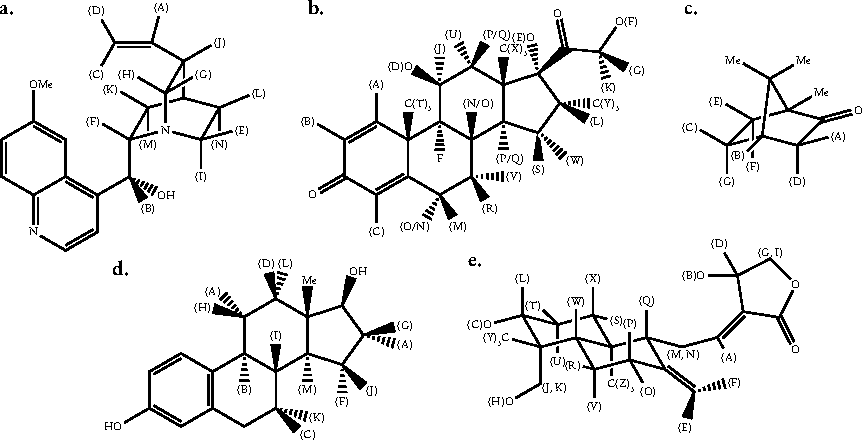
\includegraphics{structures/structures_final.pdf}
    \caption[
        The molecular structures of species giving rise to the experimental
        \acs{NMR} datasets considered in this work.
    ]{
        The molecular structures of species giving rise to the experimental
        \acs{NMR} datasets considered in this work.
        \textbf{a.} Quinine,
        \textbf{b.} Dexamethasone,
        \textbf{c.} Camphor,
        \textbf{d.} 17\textbeta-estradiol,
        \textbf{e.} Andrographolide.
        Proton environments giving rise to signals which are considered in this
        work are denoted with bracketed alphabetical characters. Non-bracketed
        alphabetical characters denote chemical symbols. \ch{Me} denotes the methyl
        group, equivalent to \ch{CH3}.
        \note{
            TODO: check assignments (esp. estradiol). If more structures need
            adding, edit the ChemDraw file on Chive called
            \path{simon_stuff/thesis_structures.cdxml}. Use EB-Garamond for
            atom labels. One a structure is made, scale to 75\% of original
            size, and set font to 7pt. Then in inkscape, rescale this by
            multiplying by 0.8.
        }
    }
    \label{fig:structures}
\end{figure}


\subsection{Diffusion datasets}
The andrographolide diffusion dataset (Figure \ref{fig:andrographolide-dosy})
was acquired using the one-shot \ac{DOSY} pulse sequence\cite{Pelta2002}
(version 1.0c, published on \formatdate{27}{03}{2012}), accessible via the webpage
\url{https://www.nmr.chemistry.manchester.ac.uk/?q=node/264}. The pulse
sequence is displayed in Figure \ref{fig:oneshot-dosy}.

\begin{figure}
    \centering
    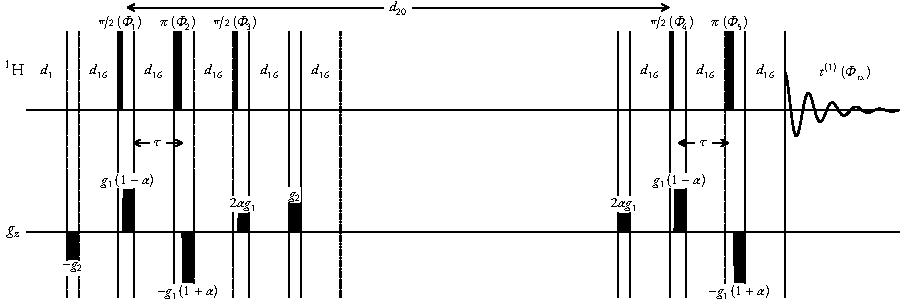
\includegraphics{oneshot_dosy_pulse_sequence/oneshot_dosy_pulse_sequence.pdf}
    \caption[
        Oneshot \acs{DOSY} pulse sequence used for the acquisition of
        andrographolide data.
    ]{
        Oneshot \ac{DOSY} pulse sequence used for the acquisition of
        andrographolide data (Figure \ref{fig:andrographolide-dosy}). All
        delays are included, though they are not to scale.
        Delays:
        $d_1$ (relaxation delay): \qty{1.5}{\second},
        $d_{16}$ (gradient recovery delay): \qty{200}{\micro\second},
        $d_{20}$ (diffusion time, equivalent to $\Delta$): \qty{0.1}{\second}.
        Hard pulses had a power of \qty{24}{\watt},
        with the duration of the $\nicefrac{\pi}{2}$ pulse being
        \qty{12}{\micro\second}.
        Diffusion encoding gradients had a smoothed square profile
        (\texttt{SMSQ10.100}), a duration of \qty{1}{\milli\second}, and had
        strengths related to the values $g_1$ and $\alpha = 0.2$.
        $g_1$ was varied across increments, with the values used
        being (\unit{\gauss \per \centi \meter}):
        6.270,
        12.470,
        16.483,
        19.695,
        22.451,
        24.905,
        27.137,
        29.200,
        31.126,
        32.939,
        34.658,
        36.296,
        37.862,
        39.367,
        40.816,
        42.215,
        43.570,
        44.883,
        46.159,
        47.401.
        Spoiler gradients had the same \texttt{SMSQ10.100} profile, had a
        duration of \qty{600}{\micro\second}, and a strength which was 75\% of
        $g_1$.
        The phase cycling scheme used was:
        $\Phi_1: 2 \times (\ang{0}, \ang{180})$;
        $\Phi_2: 4 \times \ang{0}$;
        $\Phi_3: 4 \times \ang{0}$;
        $\Phi_4: 2 \times \ang{0}, 2 \times \ang{180}$;
        $\Phi_5: 4 \times \ang{0}$;
        $\Phi_{\text{rx}}: \ang{0}, \ang{180}, \ang{180}, \ang{0}$.
    }
    \label{fig:oneshot-dosy}
\end{figure}

The glucose/valine/threonine diffusion dataset (Figure \ref{fig:gluc_val_thre})
was acquired using Bruker's \texttt{ledbpgp2s} pulse sequence (version 1.9, published on
\formatdate{19}{02}{2011}). This is a stimulated echo pulse sequence, featuring
bipolar gradients and a \ac{LED} component\cite{Wu1995}. The pulse sequence is
displayed in Figure \ref{fig:ledbpgp2s}.
\begin{figure}
    \centering
    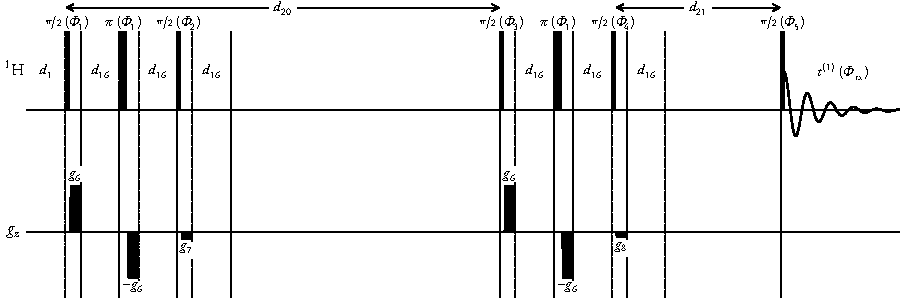
\includegraphics{ledbpgp_pulse_sequence/ledbpgp_pulse_sequence.pdf}
    \caption[
        Pulse sequence used for the acquisition of glucose/threonine/valine
        diffusion data.
    ]{
        Pulse sequence used for the acquisition of glucose/threonine/valine
        diffusion data (Figure \ref{fig:gluc_val_thre}). All
        delays are included, though they are not to scale.
        Delays:
        $d_1$ (relaxation delay): \qty{6}{\second},
        $d_{16}$ (gradient recovery delay): \qty{200}{\micro\second},
        $d_{20}$ (diffusion time, equivalent to $\Delta$): \qty{0.1}{\second},
        $d_{21}$ (eddy-current delay): \qty{5}{\milli\second}.
        Hard pulses had a power of \qty{18.204}{\watt},
        with the duration of the $\nicefrac{\pi}{2}$ pulse being
        \qty{10}{\micro\second}.
        All gradients had a smoothed square profile
        (\texttt{SMSQ10.100}).
        Gradients for diffusion encoding had a duration of
        \qty{1}{\milli\second}, with strength $g_6$ varied across increments,
        with the values used being (\unit{\gauss \per \centi \meter}):
        4.500,
        12.728,
        17.428,
        21.107,
        24.233,
        27.000,
        29.508,
        31.820,
        33.974,
        36.000.
        Spoiler gradients had a duration of \qty{600}{\micro\second}. The
        gradients had the relative strengths $g_7=-0.1713g_6$ and
        $g_8=-0.1317g_6$.
        The phase cycling scheme used was:
        $\Phi_1: 32 \times \ang{0}$;
        $\Phi_2: 8 \times (2 \times \ang{0}, 2 \times \ang{180})$;
        $\Phi_3: 2 \times (4 \times \ang{0}, 4 \times \ang{180}, 4 \times \ang{90}, 4 \times \ang{270})$;
        $\Phi_4: 2 \times (2 \times (\ang{0}, \ang{180}), 2 \times (\ang{180}, \ang{0}), 2 \times (\ang{90}, \ang{270}), 2 \times (\ang{270}, \ang{90})$;
        $\Phi_5: 2 \times (4 \times \ang{0}, 4 \times \ang{180}, 4 \times \ang{90}, 4 \times \ang{270})$;
        $\Phi_{\text{rx}}: 2 \times (\ang{0}, \ang{180}, \ang{180}, \ang{0}, \ang{180}, \ang{0} \ang{0}, \ang{180},
        \ang{270}, \ang{90}, \ang{90}, \ang{270}, \ang{90}, \ang{270}, \ang{270}, \ang{90})$.
    }
    \label{fig:ledbpgp2s}
\end{figure}

\subsection{\acs{2DJ} datasets}
\label{subsec:cupid-experimental}

The 2D J-Resolved datasets presented were acquired using Bruker's
\texttt{jresqf} pulse sequence (version 1.7, released
\formatdate{31}{01}{2012}). This pulse sequence comprises
 $\nicefrac{\pi}{2}(\Phi_1) \rightarrow \nicefrac{\tone}{2} \rightarrow
\pi(\Phi_{2}) \rightarrow \nicefrac{\tone}{2} \rightarrow \ttwo(\Phi_{\text{rx}})$, with
the EXORCYCLE phase-cycling scheme\cite[Section 11.6]{Keeler2010}:
\begin{equation*}
    \begin{array}{lllll}
        \Phi_{1}: & \ang{0} & \ang{0} & \ang{0} & \ang{0} \\
        \Phi_{2}: & \ang{0} & \ang{90} & \ang{180} & \ang{270} \\
        \Phi_{\text{rx}}: & \ang{0} & \ang{180} & \ang{0} & \ang{180}
    \end{array}
\end{equation*}
Key experiment parameters are provided in Table \ref{tab:jres_params}.

\null\vfill
\begin{table}[h!]
\centering
\begin{tabular}{ccccc}
\hline
 & Quinine & Dexamethasone & Camphor & Estradiol\\
\hline
$f_{\text{bf}}$ (\unit{\mega\hertz}) & 500.13 & 600.18 & 500.13 & 500.3\\
$\fofftwo$ (\unit{\hertz}) & 2500 & 2815.4 & 1000 & 2501.5\\
$\fswone$ (\unit{\hertz}) & 50 & 50 & 50 & 100\\
$\fswtwo$ (\unit{\hertz}) & 7500 & 7211.5 & 5000 & 5000\\
$\fswtwo$ (\unit{\partspermillion}) & 14.996 & 12.016 & 9.9974 & 9.994\\
$\None$ & 128 & 64 & 128 & 128\\
$\Ntwo$ & 16384 & 8192 & 16384 & 16384\\
NS & 4 & 2 & 4 & 4\\
DS & 4 & 8 & 4 & 2\\
PLW1 (\unit{\watt}) & 20.893 & 24 & 20.893 & 31.537\\
P1 (\unit{\micro\second}) & 10 & 12 & 10 & 15\\
D1 (\unit{\second}) & 2 & 1.5 & 2 & 1\\

\hline
\end{tabular}
\caption[
    Noteworthy experiment parameters for the 2D J-Reolved and PSYCHE experiments used.
]{
    Noteworthy experiment parameters for the 2D J-Reolved and PSYCHE experiments used.
    NS: Number of scans,
    DS: Number of dummy scans,
    PLW1: Hard pulse power (\unit{\watt}),
    P1: Duration of $\nicefrac{\pi}{2}$ pulse,
    D1: Duration of relaxation delay.
}
\label{tab:jres_params}
\end{table}
\vfill\null


\subsection{\acs{PSYCHE} datasets}
The pulse sequence used for the acquisition of the estradiol \ac{PSYCHE}
spectrum (Figure \ref{fig:estradiol-cupid}) is presented in Figure
\ref{fig:psyche}, where
pulses, gradients, and delays are described in detail. Equivalent parameters
were used for the basic setup as the estradiol 2DJ experiment, given in Table
\ref{tab:jres_params}.

The pure shift spectrum of dexamethasone (Figure
\ref{fig:dexamethasone-cupid}.a) was acquired using a \ac{TSE-PSYCHE}
experiment (Figure \ref{fig:tse_psyche}). The pulse sequence file
\texttt{UoM\_1d\_if\_tsepsyche\_ts4x} can be obtained via the link
\url{https://research.manchester.ac.uk/en/datasets/manchester-pure-shift-nmr-workshop-bruker-software}.

\begin{figure}
    \centering
    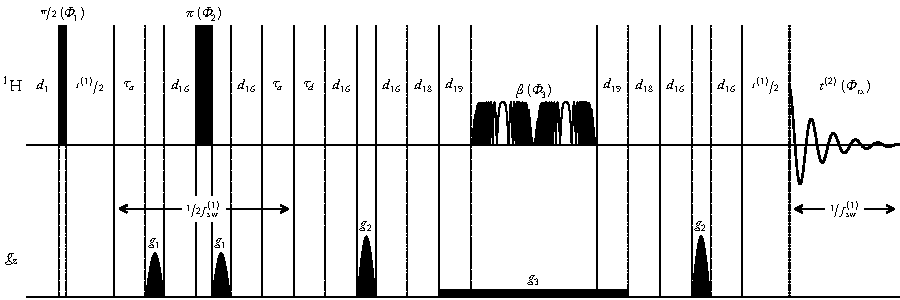
\includegraphics{psyche_pulse_sequence/psyche_pulse_sequence.pdf}
    \caption[
        \acs{PSYCHE} pulse sequence used for the acquisition of estradiol data.
    ]{
        \acs{PSYCHE} pulse sequence used for the acquisition of estradiol data. All
        delays are included, though they are not to scale.
        Delays:
        $d_1$ (relaxation delay): \qty{1}{\second},
        $d_{16}$: (gradient recovery delay): \qty{200}{\micro\second},
        $d_{18}$: \qty{200}{\micro\second},
        $d_{19}$: \qty{1}{\milli\second},
        $\tau_a$: \qty{1.3}{\milli\second},
        $\tau_d$: \qty{18.9}{\milli\second}.
        The \ac{PSYCHE} element featured two saltire chirp pulses with a
        \ac{WURST}\cite{ODell2013}
        amplitude envelope, with a target flip angle $\beta = \ang{20}$.
        Each saltire pulse
        had a bandwidth of \qty{10}{\kilo\hertz},
        a duration of \qty{25}{\milli\second},
        and a power of \qty{280}{\micro\watt}.
        Hard pulses
        had a power of \qty{31.537}{\watt},
        with the duration of the $\nicefrac{\pi}{2}$ pulse being \qty{15}{\micro\second}.
        $G_1$ and $G_2$ were gradients for coherence order selection.
        Each comprised a 100-point sine shape profile, and lasted
        \qty{1}{\milli\second}.
        $G_3$ was a rectangular weak gradient applied during the PSYCHE
        element, with a duration of \qty{52}{\milli\second}.
        The gradeint strengths as a percentage of the maximum permissible
        z-gradient were, respectively 31\%, 47\%, 1.6\%.
        The phase cycling scheme used was:
        $\Phi_1: 2 \times (\ang{0}, \ang{180})$;
        $\Phi_2: 4 \times \ang{0}$;
        $\Phi_3: 2 \times \ang{0}, 2 \times \ang{90}$;
        $\Phi_{\text{rx}}: \ang{0}, \ang{180}, \ang{180}, \ang{0}$.
    }
    \label{fig:psyche}
\end{figure}

\begin{figure}
    \centering
    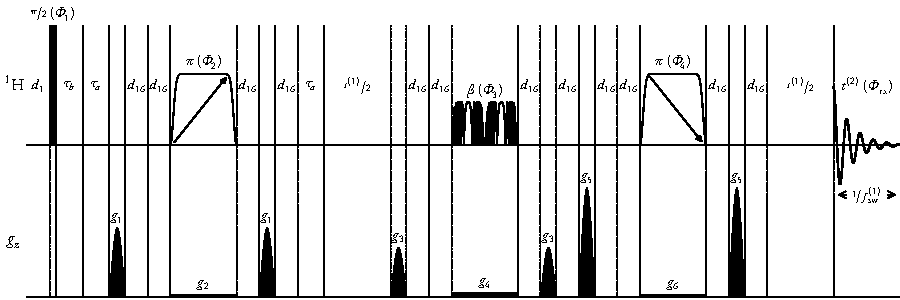
\includegraphics{tse_psyche_pulse_sequence/tse_psyche_pulse_sequence.pdf}
    \caption[
    \acs{TSE-PSYCHE} pulse sequence used for the acquisition of dexamethasone data.
    ]{
        \acs{TSE-PSYCHE} pulse sequence used for the acquisition of dexamethasone
        data (Figure \ref{fig:dexamethasone-cupid}.a).
        Delays:
        $d_1$ (relaxation delay): \qty{2}{\second},
        $d_{16}$: (gradient recovery delay): \qty{200}{\micro\second},
        $\tau_a$: \qty{5}{\milli\second} ($= \nicefrac{1}{4
        f_{\text{sw}}^{(1)}}$).
        The hard $\nicefrac{\pi}{2}$ pulse had a duration of
        \qty{12}{\micro\second}, and a power of \qty{24}{\watt}.
        The two $\pi$ pulses were unidirectional frequency-swept (chirped) pulses,
        with the first pulse sweeping from low to high frequencies, and the second
        pulse sweeping from high to low. These each had a \acs{WURST} amplitude
        envelope, lasted a duration of \qty{40}{\milli\second}, and had a power
        of $\qty{11.05}{\milli\watt}$.
        The \ac{PSYCHE} element had a target flip angle $\beta = \ang{15}$, and
        featured two saltire chirp pulses. Both saltire pulses had a
        \ac{WURST} amplitude envelope, a duration of \qty{15}{\milli\second},
        and a power of
        \qty{1.28}{\milli\watt}.
        $g_1$, $g_3$ and $g_5$ were gradients for coherence order selection.
        Each comprised a 100-point sine profile, and lasted
        \qty{1}{\milli\second}. $g_2$, $g_4$ and $g_6$ were weak rectangular gradients
        which were applied at the same time as the chirped pulses.
        The magnitudes of gradients $g_1$ to  $g_6$ as a percentage of the
        maximum permitted gradient were, respectively:
        49\%, 2\%, 35\%, 3\%, 77\%, 2\%.
        The phase cycling scheme used was:
        $\Phi_1: 8 \times \ang{0}$;
        $\Phi_2: 2 \times (2 \times \ang{0}, 2 \times \ang{180})$;
        $\Phi_3: 2 \times (\ang{0}, \ang{90}), 2 \times (\ang{180}, \ang{270})$;
        $\Phi_4: 8 \times \ang{0}$;
        $\Phi_{\text{rx}}: 4 \times (\ang{0}, \ang{180})$.
    }
    \label{fig:tse_psyche}
\end{figure}

\chapter{Miscellaneous Topics of Interest}
\label{chap:misc}

\subsection{The Nyquist Frequency}
\label{sec:nyquist}
The Nyquist frequency defines the highest frequency an oscillator can possess
such that it is sampled at least twice per period:
\begin{equation}
  f_{\mathrm{N}} = \frac{1}{2\Delta t}
\end{equation}
This quantity as at the heart of the Nyquist-Shannon Sampling Theorem, which -
in the words of Claude Shannon\cite{Shannon1949} - states:
\begin{quote}
  If a function $y(t)$ contains no frequencies
  higher than $f \si{\hertz}$, it is completely determined by giving
  its ordinates at a series of points spaced $\nicefrac{1}{2f}$ seconds
  apart.
\end{quote}
The implication of this is that the continuous FID $y(t)$ may be completely
described by its digitisation with sampling interval $\Delta t$ so long as the
frequencies $f_j$ that make it up satisfy:
\begin{equation}
  \label{permitted_freq}
  -\frac{1}{2\Delta t} \leq f_j \leq \frac{1}{2\Delta t}\ \forall j
\end{equation}
If any frequency $f_j$ does not satisfy \eqref{eq:permitted_freq}, the signal
will be insufficiently sampled, and will be spuriously represented as having a
frequency $f_a$ that satisfies
\begin{alignat}{2}
  &f_a = 2mf_{\mathrm{N}} - f_j \quad \quad &&(f_j > f_{\mathrm{N}})\\
  &f_a = 2mf_{\mathrm{N}} + f_j \quad \quad &&(f_j < -f_{\mathrm{N}}),
\end{alignat}
where $m \in \mathbb{Z}_+$. This phenomenon is called \textit{aliasing}.

\subsection{Hessian Validation}
\note{Talk about checking that my Hessian code is correct by using the finite difference method}

\subsection{Statistical Definitions}
\note{Definitions of standard error, likelihood function, ...}

% \chapter{NMR-EsPy walkthroughs}
\label{chap:walkthrough}
The remainder of this thesis is an insert from the documentation of
version 2.0 of \acs{EsPy}. The section of the documentation included provides
walkthroughs describing how to use the package's \ac{API} for the consideration
of \ac{1D} and \ac{2DJ} \ac{NMR} datasets \note{Sequential data too?}. These
walkthroughs provide a short description of the key features associated with
the package, and is an ideal first place to get up-and-running with using it.

Also included in the full documentation are instructions on installation
and using the \acp{GUI} for \ac{1D} and \ac{2DJ} estimation, and a complete
reference for the complete \ac{API}. The most up-to-date version of the
documentation can be found at:
\begin{itemize}
    \item[] \textbf{HTML:} \url{https://foroozandehgroup.github.io/NMR-EsPy/}
    \item[] \textbf{PDF:} \note{???}
\end{itemize}
The source code for \ac{EsPy} is hosted on the Foroozandeh group's GitHub page
at \url{https://github.com/foroozandehgroup/NMR-EsPy}.

\phantomsection
\stepcounter{section}
\addcontentsline{toc}{section}{\protect\numberline{\thesection}1D Walkthrough}
\sectionmark{1D Walkthrough}
\includepdf[%
    pages={13-19},%
    pagecommand={\thispagestyle{fancy}},%
    offset=0 -1cm,%
]{nmr-espy.pdf}

\phantomsection
\stepcounter{section}
\addcontentsline{toc}{section}{\protect\numberline{\thesection}2DJ Walkthrough}
\sectionmark{2DJ Walkthrough}
\includepdf[%
    pages={20-28},%
    pagecommand={\thispagestyle{fancy}},%
    offset=0 -1cm,%
]{nmr-espy.pdf}

\end{document}
